% !Mode:: "TeX:UTF-8"
\documentclass[a4paper,9pt,openleft]{book}
%\usepackage[scheme=chinese,9pt,heading]{ctex}
\usepackage{pifont}
%\usepackage{fontawesome}
\usepackage{fontspec}
\usepackage{amsmath}
\usepackage{amssymb}
\usepackage{bm}
\usepackage{array}
\usepackage{enumitem}
\usepackage{imakeidx}
\usepackage[numbers,sort&compress]{natbib}
\usepackage
[paperheight=26 true cm,paperwidth=18.4 true cm,
top=2.6 true cm,bottom=2.2 true cm,left=2.8 true cm,right=2.8 true cm]
{geometry}
\usepackage{float}
%\usepackage{setspace}
\usepackage{hyperref}
\usepackage{bookmark}
\usepackage{caption}
%\usepackage[perpage,symbol*, bottom,hang,stable,multiple]{footmisc}
\usepackage[clearempty,pagestyles]{titlesec}
\usepackage{titletoc}
\titlecontents{section}[0pt]{\addvspace{2pt}\filright}
{\contentspush{\thecontentslabel\ }}
{}{\titlerule*[8pt]{.}\contentspage}
\usepackage[cmyk,table,hyperref]{xcolor}
\usepackage{tikz}
\usepackage{tcolorbox}
\usepackage{algorithm2e}
\usepackage{listings}
\usepackage{booktabs}
\usepackage{longtable}
\usepackage{makecell}
\usepackage{tabu}
\usepackage{mdframed}
\usepackage{pdfpages}
\usepackage{qrcode}
\usepackage{threeparttable}
%\usepackage{chngcntr}
\usepackage[nottoc,chapter]{tocbibind}
\AtEndPreamble{
	\usepackage[nohyphen,strings]{underscore}
}
\usepackage{lipsum}
%
% .:: footmisc ::.
%
% Circled Digit,带圆圈数字
%\DefineFNsymbols{cd}{{\ding{172}}{\ding{173}}{\ding{174}}{\ding{175}}{\ding{176}}{\ding{177}}{\ding{178}}{\ding{179}}{\ding{180}}{\ding{181}}}
%% Negative Circled Digit,反白带圆圈数字
%\DefineFNsymbols{ncd}{{\ding{182}}{\ding{183}}{\ding{184}}{\ding{185}}{\ding{186}}{\ding{187}}{\ding{188}}{\ding{189}}{\ding{190}}{\ding{191}}}
%% Circled Sans-Serif Digit,带圆圈无衬线数字
%\DefineFNsymbols{cssd}{{\ding{192}}{\ding{193}}{\ding{194}}{\ding{195}}{\ding{196}}{\ding{197}}{\ding{198}}{\ding{199}}{\ding{200}}{\ding{201}}}
%% Negative Circled Sans-Serif Digit,反白带圆圈无衬线数字
%\DefineFNsymbols{ncssd}{{\ding{202}}{\ding{203}}{\ding{204}}{\ding{205}}{\ding{206}}{\ding{207}}{\ding{208}}{\ding{209}}{\ding{210}}{\ding{211}}}
%\setfnsymbol{cssd}
%\setlength\footnotemargin{.6em}

% package: float
\floatplacement{figure}{!ht}

% package: booktab
%\setlength\aboverulesep{0sp}
%\setlength\belowrulesep{0sp}
%\setlength\cmidrulesep{0sp}

% package: graphicx
\graphicspath{{resources/}}

% package: caption
%\DeclareCaptionFont{31104}{\FZYZK}
%\captionsetup{format=hang,labelsep=quad,font=31104}
%\DeclareCaptionFormat{31104}{%
%%	\bfseries\footnotesize#3
%\footnotesize#3
%}
%\captionsetup[lstlisting]{format=31104,singlelinecheck=off}

% package: enumitem
%\setlist{noitemsep,partopsep=0pt}%,listparindent=\parindent
%\setlist[1]{labelindent=\parindent}
%\setlist[itemize]{topsep=0pt,parsep=.5\parskip,leftmargin=1.5em}
%\setlist[itemize]{topsep=0pt,parsep=.5\parskip,leftmargin=3.5em}
%\setlist[enumerate]{topsep=0pt,parsep=.5\parskip,labelsep=*,leftmargin=1.5em}
%\setlist[enumerate,1]{topsep=0pt,parsep=.5\parskip,labelsep=*,leftmargin=3.5em}
%\setlist[description]{topsep=0pt,parsep=.5\parskip,labelsep=.25em,leftmargin=*}

% 图表编号分隔符
\makeatletter
\renewcommand\thefigure{\ifnum \c@chapter>\z@ \thechapter -\fi \@arabic\c@figure}
\renewcommand\thetable{\ifnum \c@chapter>\z@ \thechapter -\fi \@arabic\c@table}
\makeatother

%\setlength{\parskip}{2em}

% 代码风格
\lstset{ %
	language=C++,                % the language of the code
	basicstyle=\scriptsize \fontspec{Monaco},           % the size of the fonts that are used for the code
	numbers=left,                   % where to put the line-numbers
	numberstyle=\tiny\color{gray},  % the style that is used for the line-numbers
%	% will be numbered
	numbersep=5pt,                  % how far the line-numbers are from the code
	showspaces=false,               % show spaces adding particular underscores
	showstringspaces=false,         % underline spaces within strings
%	showtabs=false,                 % show tabs within strings adding particular underscores
	frame=single,                   % adds a frame around the code
%	%	rulecolor=\color{black},        % if not set, the frame-color may be changed on line-breaks within not-black text (e.g. commens (green here))
	tabsize=2,                      % sets default tabsize to 2 spaces
	%	captionpos=b,                   % sets the caption-position to bottom
	breaklines=true,                % sets automatic line breaking
%	breakatwhitespace=false,        % sets if automatic breaks should only happen at whitespace
%	title=\lstname,                   % show the filename of files included with \lstinputlisting;
	% also try caption instead of title
	keywordstyle=\textbf,          % keyword style
}

% 目录双栏
%\usepackage{multicol}
%\makeatletter
%\renewcommand\tableofcontents{%
%	\begin{multicols}{2}[%
%		\section*{%
%			\contentsname
%			\@mkboth{\MakeUppercase\contentsname}{\MakeUppercase\contentsname}}]%
%		\@starttoc{toc}%
%\end{multicols}}
%\makeatother
\makeatletter

\providecommand\optional{\stepcounter{enumi}\labelenumi\makebox[0pt][l]{$^*$}}

% +----------------------------------------------+
% : 重定义                                       :
% +----------------------------------------------+
\renewcommand{\figureautorefname}{\figurename}
\renewcommand{\tableautorefname}{\tablename}


% +----------------------------------------------+
% : 废弃命令                                     :
% +----------------------------------------------+
\def\tightlist{}

% +----------------------------------------------+
% : 取消篇标题单独页                             :
% +----------------------------------------------+
\def\@endpart{}

% +----------------------------------------------+
% : PDF属性设置                                  :
% +----------------------------------------------+
\AtEndPreamble{
	\hypersetup{
		pdfinfo={
			Title    = {\@title},
			Author   = {\@author},
			Creator  = {Adobe Acrobat 11.0},
			Producer = {Acrobat Web Capture 11.0}
		}
	}
}

% +----------------------------------------------+
% : tex.stackexchange.com/a/40363                :
% +----------------------------------------------+
\patchcmd{\@addtocurcol}%
	{\vskip \intextsep}%
	{\edef\save@first@penalty{\the\lastpenalty}\unpenalty
		\ifnum \lastpenalty = \@M % hopefully the OR penalty
			\unpenalty
		\else
			\penalty \save@first@penalty \relax % put it back
		\fi
		\ifnum \outputpenalty <-\@Mii
			\addvspace\intextsep
			\vskip\parskip
		\else
			\addvspace\intextsep
		\fi}%
	{\typeout{*** SUCCESS ***}}{\typeout{*** FAIL ***}}

\patchcmd{\@addtocurcol}%
	{\vskip\intextsep
		\ifnum \outputpenalty <-\@Mii
			\vskip -\parskip
		\fi}%
	{\ifnum \outputpenalty <-\@Mii
		\aftergroup\vskip\aftergroup\intextsep
		\aftergroup\nointerlineskip
	\else
		\vskip\intextsep
	\fi}% was the float seen in vertical mode?
	{\typeout{*** SUCCESS ***}}{\typeout{*** FAIL ***}}

\patchcmd{\@getpen}{\@M}{\@Mi}
	{\typeout{*** SUCCESS ***}}{\typeout{*** FAIL ***}}

% +----------------------------------------------+
% : Verbatim callouts                            :
% +----------------------------------------------+

% Counters for cross-referencing callouts
\newcounter{cocnt}
\newcounter{colref}

% How to represent the <co> markup.
% Big thanks to Jean-Côme Charpentier for his help.
%
\newlength{\co@width}
\newlength{\co@height}
\newlength{\balldiam}
\newlength{\ballcentre}
\newlength{\ballcenter}% 修正纵向位置

\def\conum#1{%
	\sbox{\z@}{\color{white}\sffamily\bfseries\tiny#1}% 
	% Box sizes for any number with two digits
	\sbox{\@ne}{\color{white}\sffamily\bfseries\tiny00}%
	\settowidth{\co@width}{\usebox{\@ne}}%
	\settoheight{\co@height}{\usebox{\@ne}}%
	% Find out the biggest length, to define the circle diameter
	\ifnum\co@width>\co@height
		\setlength{\balldiam}{\co@width}%
	\else
		\setlength{\balldiam}{\co@height}%
	\fi
	\balldiam=1.45\balldiam
	\ballcentre=0.5\balldiam
	\ballcenter=0.3\balldiam% 修正纵向位置
	\setlength{\unitlength}{1pt}% In the case it has been changed
	\begin{picture}(\strip@pt\balldiam,\strip@pt\balldiam) %
	\put(\strip@pt\ballcentre,\strip@pt\ballcenter){\circle*{\strip@pt\balldiam}}
	\put(\strip@pt\ballcentre,\strip@pt\ballcenter){\makebox(0,0){\usebox{\z@}}}
	\end{picture}%
}

% How to represent a <co> embedded in a listing
\def\co#1{\refstepcounter{cocnt}\conum{#1}}

% Make the <co> text and the label to link to
\def\coref#1#2{\co{#1}\label{#2}}

% Make only the <co> label to link to
\def\colabel#1{\refstepcounter{cocnt}\label{#1}}

% Make the <callout> label to link to
\def\collabel#1{\refstepcounter{colref}\label{#1}}

\makeatother


\begin{document}
\title{14 Lectures on Visual SLAM\\From Theory to Practice}
\author{Xiang Gao, Tao Zhang, Qinrui Yan and Yi Liu}
\date{\today}

\frontmatter
\maketitle
\tableofcontents

% TODO
% 统一用语:例如key frame -> keyframe, front end -> frontend, real time->real-time,等等
% \textbf 强调的地方用斜体为佳
% 检查表述和语法
% 代码的英文版分支
% 标题单词使用大写字符

% 用语:关键帧 keyframe
% 前端/后端 frontend/backend
% 视觉里程计 visual odometry
% 定位 localization 不要positioning


\mainmatter 
\addtocontents{toc}{\protect\setcounter{tocdepth}{2}}
\hypersetup{bookmarksdepth=2}
\chapter*{Preface for English Version}
A lot of friends at Github asked me about this English version. I'm really sorry it takes so long to do the translation, and I'm glad to make it publicly available to help the readers. I encountered some issues with the math equations on the web pages. Since the book is originally written in LaTeX, I'm going to release the LaTeX source along with the compiled pdf. You can directly access the pdf version for the English book, and probably the publishing house is going to help me do the paper version.

As I'm not a native English speaker, the translation work is based on Google translation and some afterward modifications. If you think the quality of translation can be improved and willing to do this, please contact me or send an issue on Github. Any help will be welcome!

Thanks for the following friend's help in the translation time: Nicolas Rosa, Carrie (Yan Ran), Collen Jones, Hong Ma. And also, thanks for your attention and support!

\vspace{5cm}
\begin{flushright}
	Xiang Gao
\end{flushright}
\chapter*{Preface}
\label{cpt:1}

\section*{What is this book talking about?}

This book introduces visual SLAM, and it is probably the first Chinese book solely focused on this specific topic.

So, what is SLAM?

SLAM stands for \textbf{S}imultaneous \textbf{L}ocalization \textbf{a}nd \textbf{M}apping. It usually refers to a robot or a moving rigid body, equipped with a specific \textbf{sensor}, estimates its \textbf{motion} and builds a \textbf{model} (certain kinds of description) of the surrounding environment, without a \textit{priori} information\cite{Davison2007}. If the sensor referred to here is mainly a camera, it is called \textbf{Visual SLAM}.

Visual SLAM is the subject of this book. We deliberately put a long definition into one single sentence so that the readers can have a clear concept. First of all, SLAM aims at solving the \textit{localization} and \textit{map building} issues at the same time. In other words, it is a problem of how to estimate the location of a sensor itself, while estimating the model of the environment. So how to achieve it? SLAM requires a good understanding of sensor information. A sensor can observe the external world in a particular form, but the specific approaches for utilizing such observations are usually different. And, why is this problem worth spending an entire book to discuss? Because it is difficult, especially if we want to do SLAM in \textbf{real-time} and \textbf{without any prior knowledge}. When we talk about visual SLAM, we need to estimate the trajectory and map based on a set of continuous images (which form a video sequence).

This seems to be quite intuitive. When we human beings enter an unfamiliar environment, aren't we doing exactly the same thing? So, the question is whether we can write programs and make computers do so. 

At the birth of computer vision, people imagined that one-day computers could act like humans, watching and observing the world and understanding the surrounding environment. The ability to explore unknown areas is a beautiful and romantic dream, attracting numerous researchers striving on this problem day and night~\cite{Hartley2003}. We thought that this would not be that difficult, but the progress turned out to be not as smooth as expected. Flowers, trees, insects, birds, and animals, are recorded so differently in computers: they are just numerical matrices consisted of numbers. To make computers understand the contents of images is as difficult as making us humans understand those blocks of numbers. We didn't even know how we understand images, nor do we know how to make computers do so. However, after decades of struggling,  we finally started to see signs of success - through Artificial Intelligence (AI) and Machine Learning (ML) technologies, which gradually enable computers to recognize objects, faces, voices, texts, although in a way (probabilistic modeling) that is still so different from us.

On the other hand, after nearly three decades of development in SLAM, our cameras begin to capture their movements and know their positions. However, there is still a massive gap between the capability of computers and humans. Researchers have successfully built a variety of real-time SLAM systems. Some of them can efficiently track their locations, and others can even do the three-dimensional reconstruction in real-time.

This is really difficult, but we have made remarkable progress. What's more exciting is that, in recent years, we have seen the emergence of a large number of SLAM-related applications. The sensor location could be very useful in many areas: indoor sweeping machines and mobile robots, self-driving cars, Unmanned Aerial Vehicles (UAVs), Virtual Reality (VR), and Augmented Reality (AR). SLAM is so important. Without it, the sweeping machine cannot maneuver in a room autonomously but wandering blindly instead; domestic robots can not follow instructions to accurately reach a specific room; Virtual reality devices will always be limited within a seat. If none of these innovations could be seen in real life, what a pity it would be.
Today's researchers and developers are increasingly aware of the importance of SLAM technology. SLAM has over 30 years of research history, and it has been a hot topic in both robotics and computer vision communities. Since the 21st century, visual SLAM technology has undergone a significant change and breakthrough in both theory and practice and is gradually moving from laboratories into the real-world. At the same time, we regretfully find that, at least in the Chinese language, SLAM-related papers and books are still very scarce, making many beginners of this area unable to get started smoothly. Although SLAM's theoretical framework has basically become mature, implementing a complete SLAM system is still very challenging and requires a high level of technical expertise. Researchers new to the area have to spend a long time learning a significant amount of scattered knowledge and often have to go through several detours to get close to the real core.

This book systematically explains the visual SLAM technology. We hope that it will (at least partially) fill the current gap. We will detail SLAM's theoretical background, system architecture, and the various mainstream modules. At the same time, we emphasize the practice: all the essential algorithms introduced in this book will be provided with runnable code that can be tested by yourself so that readers can reach a more in-depth understanding. Visual SLAM, after all, is a technology for real applications. Although the mathematical theory can be beautiful, if you cannot convert it into code, it will be like a castle in the air, bringing little practical impact. We believe that practice brings real knowledge (and true love). After getting your hands dirty with the algorithms, you can truly understand SLAM and claim that you have fallen in love with SLAM research.

Since its inception in 1986~\cite{Smith1986}, SLAM has been a hot research topic in robotics. It is very difficult to provide a complete introduction to all the algorithms and their variants in the SLAM history, and we consider it unnecessary as well. This book will first introduce the background knowledge, such as the 3D geometry, computer vision, state estimation theory, Lie Group/Lie algebra, etc. We will show the trunk of the SLAM tree and omit those complicated and oddly-shaped leaves. We think this is effective. If the reader can master the trunk's essence, they have already gained the ability to explore the frontier research details. So we aim to help SLAM beginners quickly grow into qualified researchers and developers. On the other hand, even if you are already an experienced SLAM researcher, this book may reveal areas that you are unfamiliar with and provide you with new insights.

There have already been a few SLAM-related books around, such as \textit{Probabilistic Robotics}~\cite{Thrun2005}, \textit{Multiple View Geometry in Computer Vision}~\cite{Hartley2003}, \textit{State Estimation for Robotics: A Matrix-Lie-Group Approach}~\cite{Barfoot2016}, etc. They provide rich content, comprehensive discussions, and rigorous derivations, and therefore are the most popular textbooks among SLAM researchers. However,  there are two critical issues: Firstly, the purpose of these books is often to introduce the fundamental mathematical theory, with SLAM being only one of its applications. Therefore, they cannot be considered as specifically visual SLAM focused. Secondly, they place great emphasis on mathematical theory but are relatively weak in programming. This makes readers still fumbling when trying to apply the knowledge they learn from the books. Our belief is: one can only claim a real understanding of a problem only after coding, debugging, and tweaking algorithms and parameters with his own hands.

This book will introduce the history, theory, algorithms, and research status in SLAM and explain a complete SLAM system by decomposing it into several modules: \textit{visual odometry}, \textit{backend optimization}, \textit{map building}, and \textit{loop closure detection}. We will accompany the readers step by step to implement each core algorithm, discuss why they are effective, under what situations they are ill-conditioned, and guide them by running the code on your own machines. You will be exposed to the critical mathematical theory and programming knowledge and will use various libraries including \textit{Eigen}, \textit{OpenCV}, \textit{PCL}, \textit{g2o}, and \textit{Ceres}, and learn their usage in Linux.

Well, enough talking, wish you a pleasant journey!

\section*{How to Use This Book?}

This book is entitled as \textit{Basic Knowledge on Visual SLAM\\From Theory to Practice}. We will organize the contents into lectures like studying in a classroom. Each lecture focuses on one specific topic, organized in a logical order. Each chapter will include both a \textit{theoretical} part and a \textit{practical} part, with the theoretical usually coming first. We will introduce the mathematics essential to understand the algorithms, and most of the time in a narrative way, rather than in a \textit{definition, theorem, inference} approach adopted by most mathematical textbooks. We think this will be much easier to understand, but of course, with the price of being less rigorous sometimes. In practical parts, we will provide code, discuss the various components' meaning, and demonstrate some experimental results. So, when you see chapters with the word practice in the title, you should turn on your computer and start to program with us, joyfully.

The book can be divided into two parts: The first part will be mainly focused on fundamental math knowledge, which contains:
\begin{enumerate}
	\item Preface (the one you are reading now), introducing the book's contents and structure.
	\item Lecture \ref{cpt:2}: an overview of a SLAM system. It describes each module of a typical SLAM system and explains what to do and how to do it. The practice section introduces basic C++ programming in a Linux environment and the use of an IDE.
	\item Lecture \ref{cpt:3}: rigid body motion in 3D space. You will learn about rotation matrices, quaternions, Euler angles and practice them with the \textit{Eigen} library.
	\item Lecture \ref{cpt:4}: Lie group and Lie algebra. It doesn't matter if you have never heard of them. You will learn the basics of the Lie group and manipulate them with \textit{Sophus}.
	\item Lecture \ref{cpt:5}: pinhole camera model and image expression in computer. You will use \textit{OpenCV} to retrieve the camera's intrinsic and extrinsic parameters and generate a point cloud using the depth information through \textit{PCL} (Point Cloud Library).
	\item Lecture \ref{cpt:6}: nonlinear optimization, including state estimation, least squares, and gradient descent methods, e.g., Gauss-Newton and Levenburg-Marquardt method. You will solve a curve-fitting problem using the \textit{Ceres} and \textit{g2o} library.
	
	From lecture \ref{cpt:7}, we will be discussing SLAM algorithms, starting with visual odometry (VO) and followed by the map building problems: 
	
	\item Lecture \ref{cpt:7}: feature-based visual odometry, which is currently the mainstream in VO. Contents include feature extraction and matching, epipolar geometry calculation, Perspective-n-Point (PnP) algorithm, Iterative Closest Point (ICP) algorithm, and Bundle Adjustment (BA), etc. You will run these algorithms either by calling \textit{OpenCV} functions or constructing your own optimization problem in \textit{Ceres} and \textit{g2o}.

	\item Lecture \ref{cpt:8}: direct (or intensity-based) method for VO. You will learn the optical flow principle and the direct method. The practice part is about writing single-layer and multi-layer optical flow and direct method to implement a two-view VO.
	
	\item Lecture \ref{cpt:9}: backend optimization. We will discuss Bundle Adjustment in detail and show the relationship between its sparse structure and the corresponding graph model. You will use \textit{Ceres} and \textit{g2o} separately to solve the same BA problem.
	
	\item Lecture \ref{cpt:backend2}: pose graph in the backend optimization. Pose graph is a more compact representation for BA, which converts all map points into constraints between keyframes. You will use \textit{g2o} to optimize a pose graph.
	
	\item Lecture \ref{cpt:11}: loop closure detection, mainly Bag-of-Word (BoW) based method. You will use DBoW3 to train a dictionary from images and detect loops in videos. 
	
	\item Lecture \ref{cpt:12}: map building. We will discuss how to estimate the depth of pixels in monocular SLAM  (and show why they are unreliable). Compared with monocular depth estimation, building a dense map with RGB-D cameras is much easier. You will write programs for epipolar line search and patch matching to estimate depth from monocular images and then build a point cloud map and octagonal treemap from RGB-D data.
	
	\item Lecture \ref{cpt:13}: a practice chapter for stereo VO. You will build a visual odometry framework by yourself by integrating the previously learned knowledge and solve problems such as frame and map point management, keyframe selection, and optimization control.
	
	\item Lecture \ref{cpt:14}: current open-source SLAM projects and future development direction. We believe that after reading the previous chapters, you can understand other people's approaches easily and be capable of achieving new ideas of your own.
\end{enumerate}

Finally, if you don't understand what we are talking about at all, congratulations! This book is right for you! 

\section*{Source Code}

All source code in this book is hosted on Github:

{\hfill\url{https://github.com/gaoxiang12/slambook2}\hfill}

Note the \textit{slambook2} refers to the second version in which we added a lot of extra experiments.

Check out the English version by:
{\hfill git checkout -b en origin-en\hfill}

It is strongly recommended that readers download them for viewing at any time. The code is divided into chapters. For example, the contents of the \textit{7th} lecture will be placed in folder \textit{ch7}. Some of the small libraries used in the book can be found in the ``3rdparty'' folder as compressed packages. For large and medium-sized libraries like \textit{OpenCV}, we will introduce their installation methods when they first appear. If you have any questions regarding the code, click the \textit{issue} button on GitHub to submit. If there is indeed a problem with the code, we will correct them in time. If you are not accustomed to using Git, you can also click the  \textit{Download} button on the right side to download a zipped file to your local drive.

\section*{Targeted Readers}

This book is for students and researchers interested in SLAM. Reading this book needs specific prerequisites, we assume that you have the following knowledge:

\begin{itemize}
	\item Calculus, Linear Algebra, Probability Theory. These are the fundamental mathematical knowledge that most readers should have learned during undergraduate study. You should at least understand what a matrix and a vector are, and what it means by doing differentiation and integration. For more advanced mathematical knowledge required, we will introduce in this book as we proceed.
	\item Basic C++ Programming. As we will be using C++ as our major programming language, it is recommended that the readers are at least familiar with its basic concepts and syntax. For example, you should know what a class is, how to use the C++ standard library, how to use template classes, etc. We will try our best to avoid using tricks, but we really can not avert them in certain situations. We will also adopt some of the C++11 standards, but don't worry. They will be explained if necessary.
	
	\item Linux Basics. Our development environment is Linux instead of Windows, and we will only provide source code for Linux. We believe that mastering Linux is an essential skill for SLAM researchers, and please  don't ask for Windows related issues. After going through this book's contents, we think you will agree with us \footnote{Linux is not that popular in China as our computer science education starts very lately around the 1990s.}. In Linux, the configuration of related libraries is so convenient, and you will gradually appreciate the benefit of mastering it. If you have never used a Linux system, it will be beneficial to find some Linux learning materials and spend some time reading them (the first few chapters of an introductory book should be sufficient). We do not ask readers to have superb Linux operating skills, but we do hope readers know how to find a terminal and enter a code directory. There are some self-test questions on Linux at the end of this chapter. If you have answers to them, you should be able to quickly understand the code in this book.
\end{itemize}

Readers interested in SLAM but do not have the knowledge mentioned above may find it difficult to proceed with this book. If you do not understand the basics of C++, you can read some introductory books such as \textit{C ++ Primer Plus}. If you do not have the relevant math knowledge, we also suggest reading some relevant math textbooks first. Nevertheless, most readers who have completed undergraduate study should already have the necessary mathematical backgrounds. Regarding the code, we recommend that you spend time typing them by yourself and tweaking the parameters to see how they affect outputs. This will be very helpful.

This book can be used as a textbook for SLAM-related courses or as self-study materials.

\section*{Style}

This book covers both mathematical theory and programming implementation. Therefore, for the convenience of reading, we will be using different layouts to distinguish the contents.

\begin{enumerate}
	\item Mathematical formulas will be listed separately, and important formulas will be assigned with an equation number on the right end of the line, for example:
	
	\begin{equation}
	\mathbf{y} =\mathbf{A}\mathbf{x}.
	\end{equation}
	
	Italics are used for scalars like $a$. Bold symbols are used for vectors and matrices like $\mathbf{a}, \mathbf{A}$. Hollow bold represents special sets, e.g., the real number set $\mathbb{R}$ and the integer set $\mathbb{Z}$. Gothic is used for Lie Algebra, e.g., $\mathfrak{se}(3)$.
	
	\item Source code will be framed into boxes, using a smaller font size, with line numbers on the left. If a code block is long, the box may continue to the next page:
	\begin{lstlisting}[language=C++,caption=Code example:]
	#include <iostream>
	using namespace std;

	int main (int argc, char** argv) {
		cout << "Hello" << endl;
		return 0;
	}
	\end{lstlisting}
	
	\item When the code block is too long or contains repeated parts with previously listed code, it is not appropriate to be listed entirely. We will only give the important parts and mark them with \textit{part}. Therefore, we strongly recommend that readers download all the source code on GitHub and complete the exercises to better understand the book.
	
	\item Due to typographical reasons, the book's code may be slightly different from the code in GitHub. In that case, please use the code on GitHub.
	
	\item For each of the libraries we use, it will be explained in detail when first appearing but not repeated in the follow-up. Therefore, it is recommended that readers read this book in order.
	
	\item A \textit{goal of study} part will be presented at the beginning of each lecture. A summary and some exercises will be given at the end. The cited references are listed at the end of the book.

	\item The chapters with an asterisk mark in front are optional readings, and readers can read them according to their interests. Skipping them will not hinder the understanding of subsequent chapters.
	
	\item Important contents will be marked in \textbf{bold} or \emph{italic}, as we are already accustomed to.

	\item Most of the experiments we designed are demonstrative. Understanding them does not mean that you are already familiar with the entire library. Otherwise, this book will be an \textit{OpenCV} or \textit{PCL} document. So we recommend that you spend time on yourselves in further exploring the important libraries frequently used in the book.

	\item The book's exercises and optional readings may require you to search for additional materials, so you need to learn to use search engines.
\end{enumerate}

\section*{Exercises (Self-test Questions)}
\begin{enumerate}
	\item Suppose we have a linear equation $\mathbf{Ax}=\mathbf{b}$. If $\mathbf{A}$ and $\mathbf{b}$ are known, how to solve the $\mathbf{x}$? What are the requirements for $\mathbf{A}$ and $\mathbf{b}$ if we want a unique $\mathbf{x}$? (Hint: check the rank of $\mathbf{A}$ and $\mathbf{b}$).
	
	\item What is a Gaussian distribution? What does it look like in a one-dimensional case? How about in a high-dimensional case?
	
	\item What is the \textbf{class} in C++? Do you know STL? Have you ever used them?
	
	\item How do you write a C++ program? (It's completely fine if your answer is ``using Visual C++ 6.0'' \footnote{As I know, many of our undergraduate students are still using this version of VC++ in the university. }).
	
	\item Do you know the C++11 standard? Which new features have you heard of or used? Are you familiar with any other standard?
	
	\item Do you know Linux? Have you used at least one of the popular distributions (not including Android), such as Ubuntu?
	
	\item What is the directory structure of Linux? What basic commands do you know? (e.g., \textit{ls}, \textit{cat}, etc.)
	
	\item How to install the software in Ubuntu (without using the Software Center)? What directories are software usually installed under? If you only know the fuzzy name of a software (for example, you want to install a library with the word ``eigen'' in its name), how to search it?
	
	\item *Spend an hour learning \textit{vim}. You will be using it sooner or later. You can \textit{vimtutor} into a terminal and read through its contents. We do not require you to operate it very skillfully, as long as you can use it to edit the code in the process of learning this book. Do not waste time on its plugins for now. Do not try to turn vim into an IDE. We will only use it for text editing in this book.
	
\end{enumerate}

% !Mode:: "TeX:UTF-8"
\chapter{First Glance of Visual SLAM}
\begin{mdframed}
	\textbf{Goal of Study}
	\begin{enumerate}[labelindent=0em,leftmargin=1.5em]
		\item Understand which modules a visual SLAM framework consists of, and what task each module carries out.
		\item Set up the programming environment, and prepare for experiments.
		\item Understand how to compile and run a program under Linux. If there is a problem, how to debug it.
		\item Learn the basic usage of cmake.
	\end{enumerate}
\end{mdframed}

\newpage
\section{Introduction}

This lecture summarizes the structure of a visual SLAM system as an outline of subsequent chapters. Practice part introduces the fundamentals of environment setup and program development. We will make a small "Hello SLAM" program at the end.

\section{Meet "Little Carrot"}

Suppose we assembled a robot called \emph{Little Carrot}, as shown in the following figure:

\begin{figure}
	\centering
	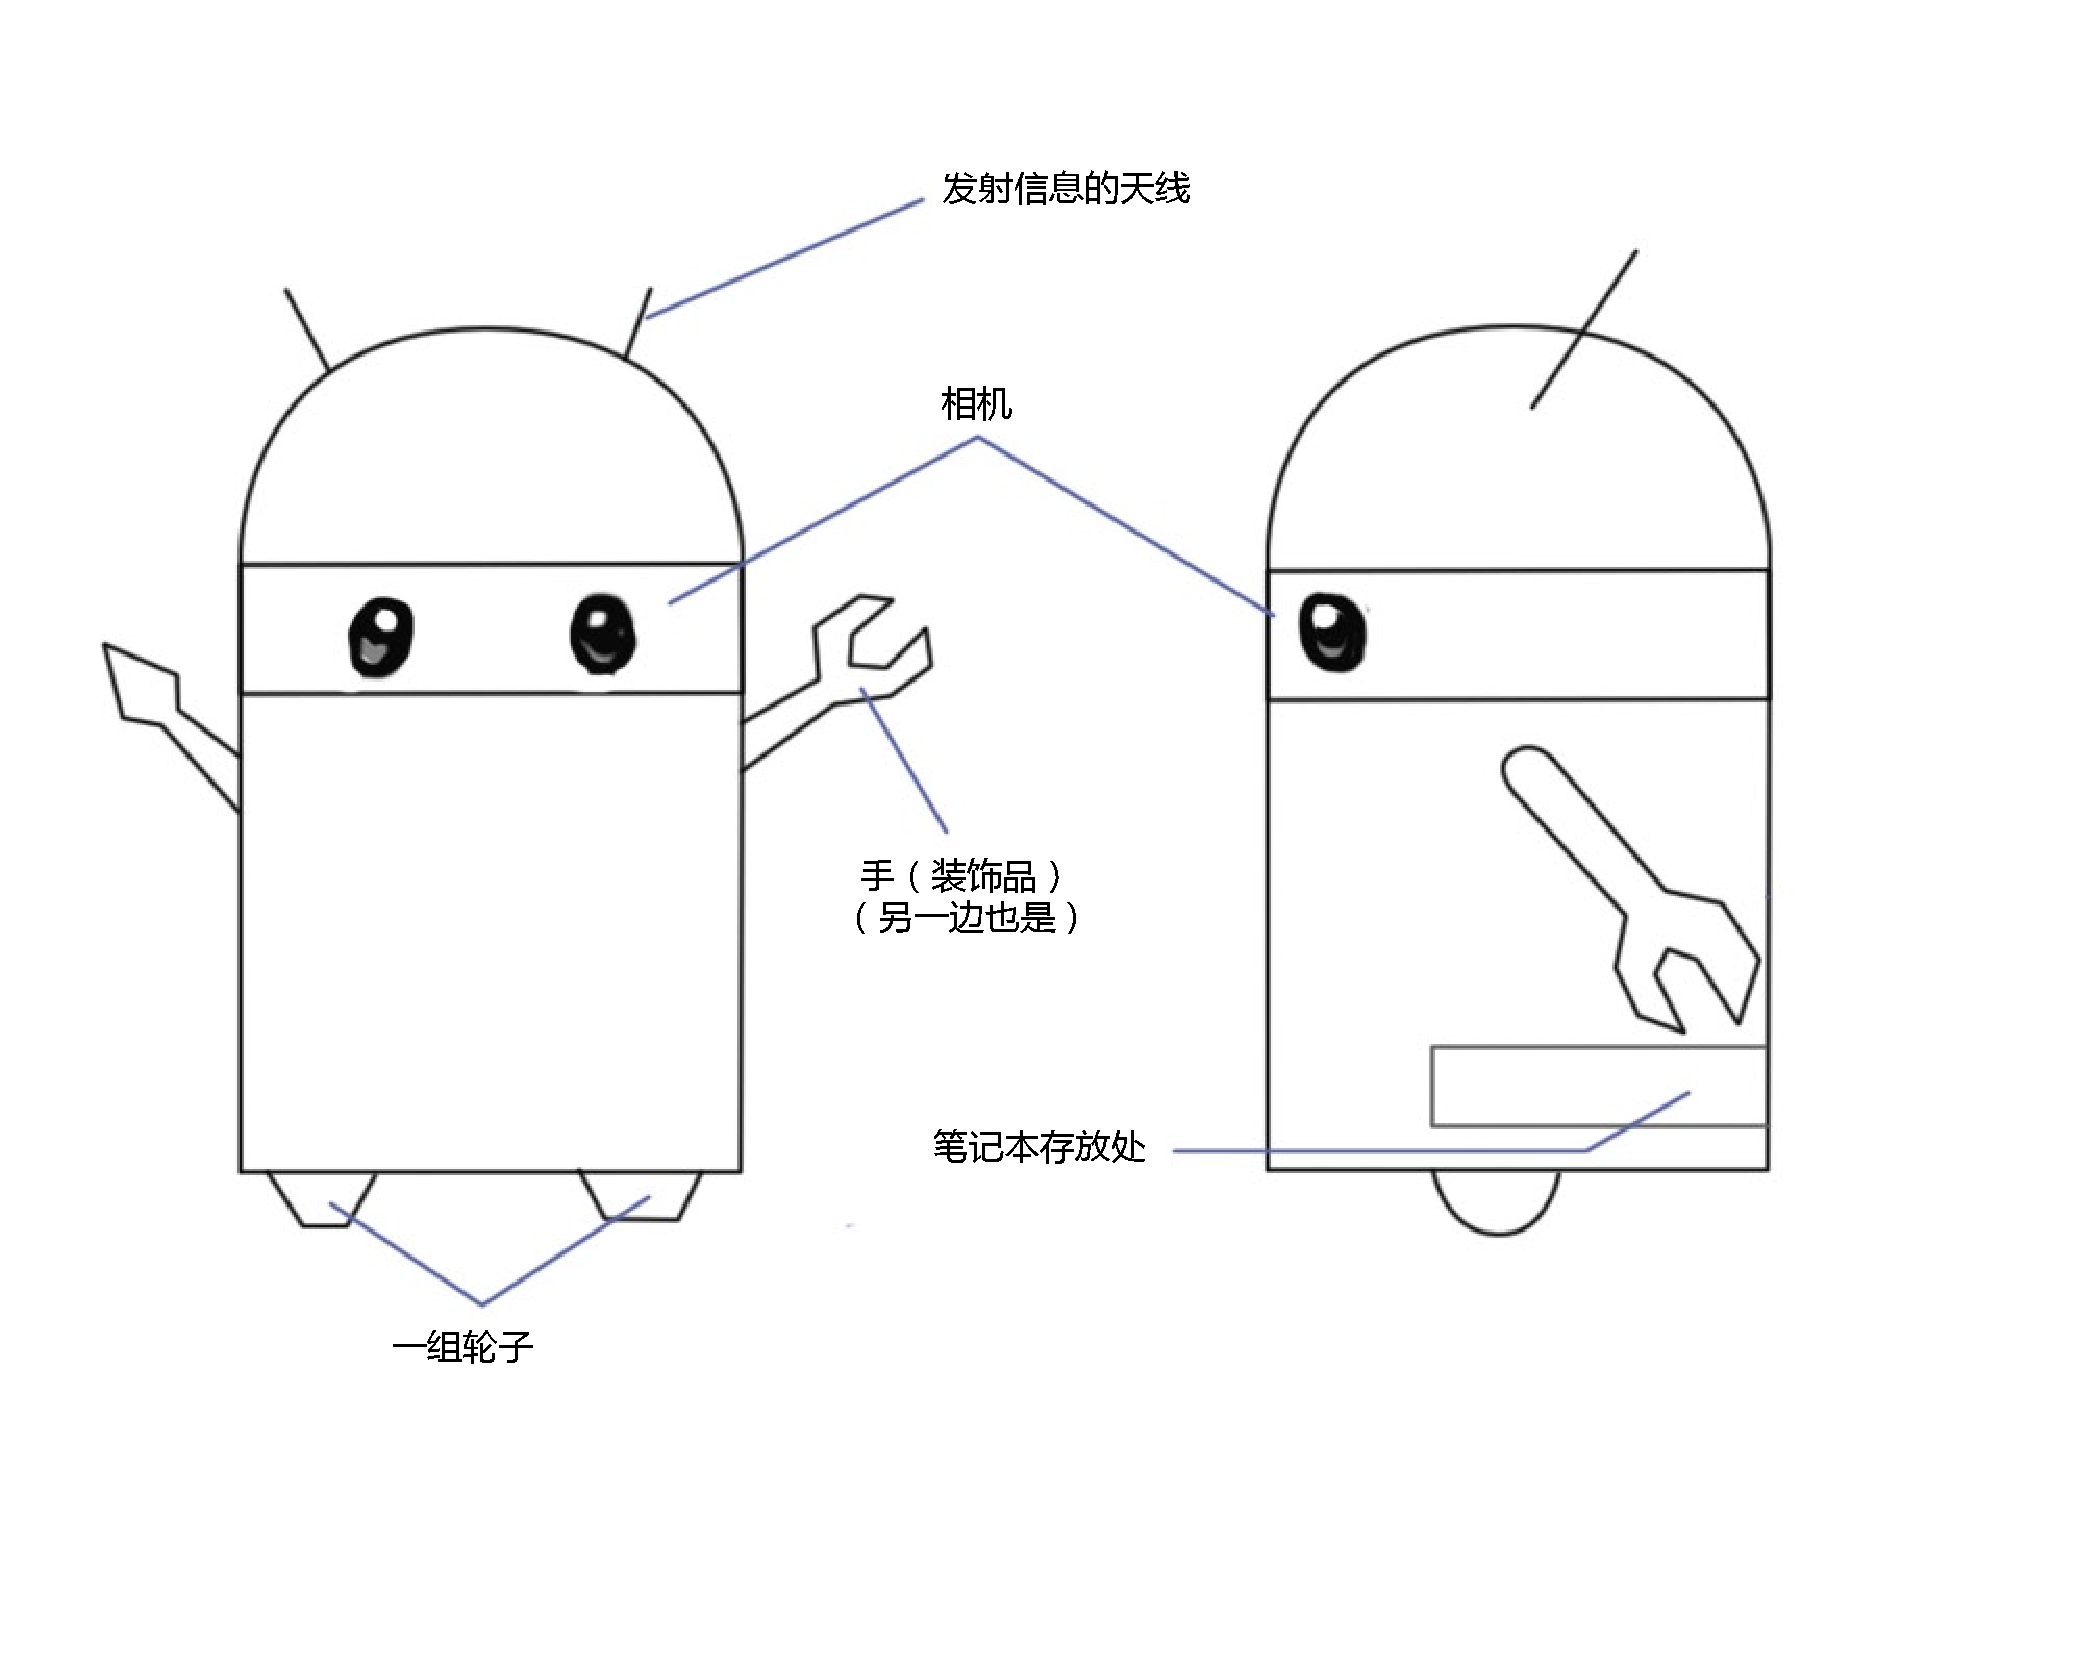
\includegraphics[width=0.8\textwidth]{resources/whatIsSLAM/carrot.pdf}
	\caption{The sketch of robot \emph{Little Carrot}}
\end{figure}

Although it looks a bit like the Android robot, it has nothing to do with the Android system. We put a laptop into its trunk (so that we can debug programs at any time). So, what is our robot capable to do?

We hope Little Carrot has the ability of \emph{autonomous moving}. Although there are many \emph{robots} placed statically on desktops, capable of chatting with people or playing music, but a tablet computer nowadays can also deliver the same tasks. As a robot, we hope Little Carrot can move freely in a room. Wherever we say hello to it, it can come to us right away.

First of all, such a robot needs wheels and motors to move, so we installed wheels under Little Carrot (gait control for humanoid robots is very complicated, which we will not be considering here). Now with the wheels, the robot is able to move, but without an effective navigation system, Little Carrot does not know where a target of action is, and it can do nothing but wander around blindly. Even worse, it may hit a wall and cause damage. In order to avoid this, we installed cameras on its head, with the intuition that such a robot \emph{should look similar to human}. Certainly, with eyes, brains and limbs, human can walk freely and explore any environment, so we (somehow naively) think that our robot should be able to achieve it too. Well, in order to make Little Carrot able to explore a room, we find it at least needs to know two things:

\begin{enumerate}
	\item  Where am I? - It's about \emph{localization}.
	\item What is the surrounding environment like? -It's about \emph{map building}.
\end{enumerate}

\emph{Localization} and \emph{map building}, can be seen as the perception in both inward and outward directions. As a completely autonomous robot, Little Carrot need not only to understand its own \emph{state} (i.e. the location), but also the external \emph{environment} (i.e. the map). Of course, there are many different approaches to solve these two problems. For example, we can lay guiding rails on the floor of the room, or paster a lot of artificial markers such as QR code pictures on the wall, or mount radio positioning devices on the table. If you are outdoor, you can also install a GNSS receiver (like the one in a cell phone or a car) on the head of Little Carrot. With these devices, can we claim that the positioning problem has been resolved? Let's categorize these sensors (see Fig.~\ref{fig:sensors}) into two classes.

\begin{figure}
	\centering
	\includegraphics[width=0.8\textwidth]{./resources/whatIsSLAM/sensors.jpg}
	\caption{Different kinds of sensors: (a) QR code (b) GNSS receiver (c) guiding rails (d) Laser range finder (e) Inertial measurement unit (f) stereo camera }
	\label{fig:sensors}
\end{figure}

The first class are \emph{non-intrusive} sensors which are completely self-contained inside a robot, such as wheel encoders, cameras, laser scanners, etc. They do not assume an cooperative environment around the robot. The other class are \emph{intrusive} sensors depending on a prepared environment, such as the above mentioned guiding rails, QR codes, etc. Intrusive sensors can usually locate a robot directly, solving the positioning problem in a simple and effective manner. However, since they require changes on the environment, the scope of usage is often limited within a certain degree. For example, if there is no GPS signal, or guiding rails cannot be laid, what should we do in those cases?

We can see that the intrusive sensors place certain \emph{constraints} to the external environment. A localization system based on them can only function properly when those constraints are met in the real world. Otherwise, the localization approach cannot be carried out anymore, like GPS positioning system normally doesn't work well in indoor environments. Therefore, although this type of sensor is simple and reliable, they do not work as a general solution. In contrast, non-intrusive sensors, such as laser scanners, cameras, wheel encoders, Inertial Measurement Units (IMUs), etc., can only observe indirect physical quantities rather than the direct locations. For example, a wheel encoder measures the wheel rotation angle, an IMU measures the angular velocity and the acceleration, a camera or a laser scanner observe the external environment in a certain form like point-clouds and images. We have to apply algorithms to infer positions from these indirect observations. While this sounds like a roundabout tactic, the more obvious benefit is that it does not make any demands on the environment, making it possible for this localization framework to be applied to an unknown environment. Therefore, they are called as self-localization in many research area.

Looking back at the SLAM definitions discussed earlier, we emphasized an \emph{unknown environment} in SLAM problems. In theory, we should not presume which environment the Little Carrot will be used (but in reality we will have a rough range, such as indoor or outdoor), which means that we can not assume that the external sensors like GPS can work smoothly. Therefore, the use of portable non-intrusive sensors to achieve SLAM is our main focus. In particular, when talking about visual SLAM, we generally refer to the using of \emph{cameras} to solve the localization and map building problems.

Visual SLAM is the main subject of this book, so we are particularly interested in what the Little Carrot's eyes can do. The cameras used in SLAM are different from the commonly seen SLR cameras. It is often much simpler and does not carry expensive lens. It shoots at the surrounding environment at a certain rate, forming a continuous video stream. An ordinary camera can capture images at 30 frames per second, while high-speed cameras can do faster. The camera can be roughly divided into three categories: Monocular, Stereo and RGB-D, as shown by the following figure \ref{fig:cameras}. Intuitively, a monocular camera has only one camera, a stereo camera has two. The principle of a RGB-D camera is more complex, in addition to being able to collect color images, it can also measure the distance of the scene from the camera for each pixel. RGB-D cameras usually carry multiple cameras, and may adopt a variety of different working principles. In the fifth lecture, we will detail their working principles, and readers just need an intuitive impression for now. In addition, there are also specialty and emerging camera types can be applied to SLAM, such as panorama camera \cite{Pretto2011}, event camera \cite{Rueckauer2016}. Although they are occasionally seen in SLAM applications, so far they have not become the mainstream. From the appearance we can infer that Little Carrot seems to carry a stereo camera.

\begin{figure}
	\centering
	\includegraphics[width=0.8\textwidth]{./resources/whatIsSLAM/camera.pdf}
	\caption{Different kinds of cameras: monocular, RGB-D and stereo. }
	\label{fig:cameras}
\end{figure}

Now, let's take a look at the pros and cons of using different type of camera for SLAM.

\subsubsection{Monocular Camera}

The SLAM system that uses only one camera is called Monocular SLAM. This sensor structure is particularly simple, and the cost is particularly low, therefore the monocular SLAM has been very attractive to researchers. You must have seen the output data of a monocular camera: photo. Yes, as a photo, what are its characteristics?

A photo is essentially a \emph{projection} of a scene onto a camera's imaging plane. It reflects a three-dimensional world in a two-dimensional form. Obviously, there is one dimension lost during this projection process, which is the so-called depth (or distance). In a monocular case, we can not obtain the \emph{distance} between objects in the scene and the camera by using a single image. Later we will see that this distance is actually critical for SLAM. Because we human have seen a large number of images, we formed a natural sense of distances for most scenes, and this can help us determine the distance relationship among the objects in the image. For example, we can recognize objects in the image and correlate them with their approximate size obtained from daily experience. The close objects will occlude the distant objects; the sun, the moon and other celestial objects are infinitely far away; an object will have shadow if it is under sunlight. This common sense can help us determine the distance of objects, but there are also certain cases that confuse us, and we can no longer determine the distance and true size of an object. The following figure \ref{fig:why-depth} is shown as an example. In this image, we can not determine whether the figures are real person or small toys purely based on the image itself. Unless we change our view angle, explore the three-dimensional structure of the scene. In other words, from a single image, we can not determine the true size of an object. It may be a big but far away object, but it may also be a close but small object. They may appear to be the same size in an image due to the perspective projection effect.

\begin{figure}
	\centering
	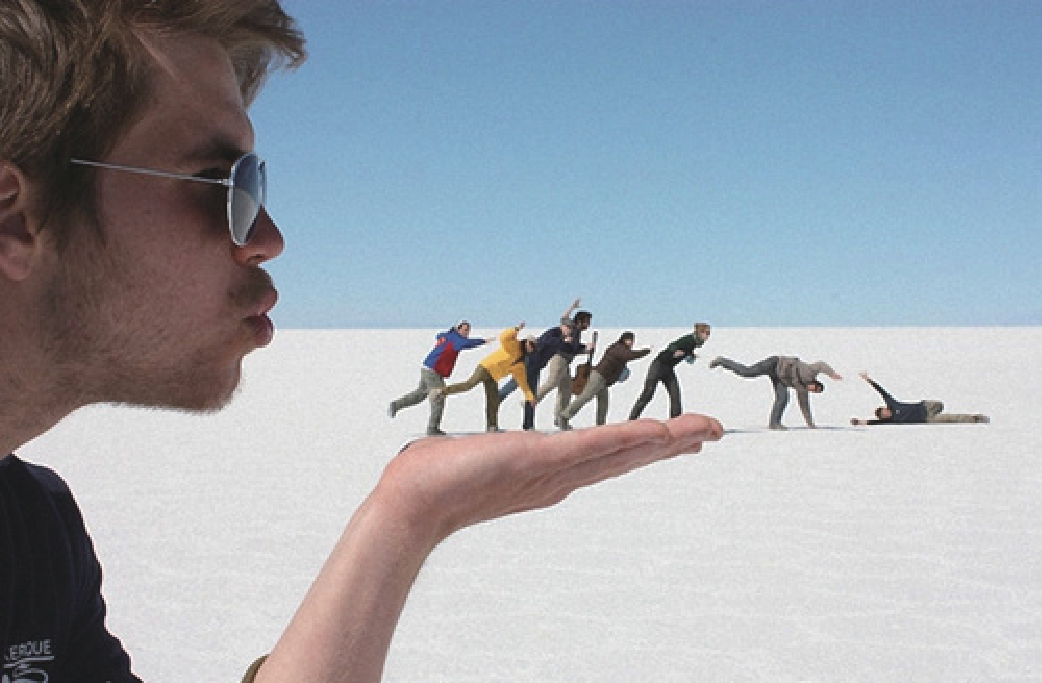
\includegraphics[width=0.8\textwidth]{./resources/whatIsSLAM/why-depth.pdf}
	\caption{We cannot tell if the people are real humans or just small toys from a single image}
	\label{fig:why-depth}
\end{figure}

Since the image taken by an monocular camera is just a 2D projection of the 3D space, if we want to recover the 3D structure, we have to change the camera's view angle. Monocular SLAM adopts the same principle. We move the camera and estimate its own \emph{motion}, as well as the distances and sizes of the objects in the scene, namely the \emph{structure} of the scene. So how should we estimate these movements and structures? From the everyday experience we know that if a camera moves to the right, the objects in the image will move to the left which gives us an inspiration of inferring motion. On the other hand, we also know that closer objects move faster, while distant objects move slower. Thus, when the camera moves, the movement of these objects on the image forms pixel disparity. Through calculating the disparity, we can quantitatively determine which objects are far away and which objects are close.

However, even if we know which objects are near and which are far, they are still only relative values. For example, when we are watching a movie, we can tell which objects in the movie scene are bigger than the others, but we can not determine the \emph{real size} of those objects -- are the buildings real high-rise buildings or just models on a table? Is it a real monster that destructs a building, or just an actor wearing special clothing? Intuitively, if the camera's movement and the scene size are doubled at the same time, monocular cameras see the same. Likewise, multiplying this size by any factor, we will still get the same picture. This demonstrates that the trajectory and map obtained from monocular SLAM estimation will differ from the actual trajectory and map with a factor, which is just the so-called \emph{scale} \footnote{Mathematical reason will be explained in the visual odometry chapter.}. Since monocular SLAM can not determine this real scale purely based on images, this is also called the \emph{scale ambiguity}.

In monocular SLAM, depth can only be calculated with translational movement, and the real scale cannot be determined. These two things could cause significant trouble when applying monocular SLAM into real-world applications. The fundamental cause is that depth can not be determined from a single image. So, in order to obtain real-scaled depth, we start to use stereo and RGB-D cameras.

\subsubsection{Stereo Camera and RGB-D Camera}
The purpose of using stereo and RGB-D cameras is to measure the distance between objects and the camera, to overcome the shortcomings of monocular cameras that distances are unknown. Once distances are known, the 3D structure of a scene can be recovered from a single frame, and also eliminates the scale ambiguity. Although both stereo and RGB-D cameras are able to measure the distance, their principles are not the same. A stereo camera consists of two synchronized monocular cameras, displaced with a known distance, namely the \emph{baseline}. Because the physical distance of the baseline is know, we are able to calculate the 3D position of each pixel, in a way that is very similar to our human eyes. We can estimate the distances of the objects based on the differences between the images from left and right eye, and we can try to do the same on computers (see Fig.~\ref{fig:stereo}). We can also extend stereo camera to multi-camera systems if needed, but basically there is no much difference.

\begin{figure}
    \centering
    \includegraphics[width=0.8\textwidth]{./resources/whatIsSLAM/stereo.pdf}
    \caption{Distance is calculated from the disparity of two stereo image pair.}
    \label{fig:stereo}
\end{figure}


Stereo cameras usually require significant amount of computational power to (unreliably) estimate depth for each pixel. This is really clumsy compared to human beings. The depth range measured by a stereo camera is related to the baseline length. The longer a baseline is, the farther it can measure. So stereo cameras mounted on autonomous vehicles are usually quite big. Depth estimation for stereo cameras is achieved by comparing images from the left and right cameras, and does not rely on other sensing equipment. Thus stereo cameras can be applied both indoor and outdoor. The disadvantage of stereo cameras or multi-camera systems is that the configuration and calibration process is complicated, and their depth range and accuracy are limited by baseline length and camera resolution. Moreover, stereo matching and disparity calculation also consumes much computational resource, and usually requires GPU or FPGA to accelerate in order to generate real-time depth maps. Therefore, in most of the state-of-the-art algorithms, computational cost is still one of the major problems of stereo cameras.

Depth camera (also known as RGB-D camera, RGB-D will be used in this book) is a type of new cameras rising since 2010. Similar to laser scanners, RGB-D cameras adopt infrared structure of light or Time-of-Flight (ToF) principles, and measure the distance between objects and the camera by actively emitting light to the object and receive the returned light. This part is not solved by software as a stereo camera, but by physical sensors, so it can save much computational resource compared to stereo cameras (see Fig.~\ref{fig:RGBD}). Common RGB-D cameras include Kinect / Kinect V2, Xtion Pro Live, RealSense, etc. However, most of the RGB-D cameras still suffer from issues including narrow measurement range, noisy data, small field of view, susceptible to sunlight interference, and unable to measure transparent material. For SLAM purpose, RGB-D cameras are mainly used in indoor environments, and are not suitable for outdoor applications.
\begin{figure}
    \centering
    \includegraphics[width=0.8\textwidth]{./resources/whatIsSLAM/rgbd.pdf}
    \caption{RGBD cameras measure the distance and can build a point cloud with a single image frame.}
    \label{fig:RGBD}
\end{figure}

We have discussed the common types of cameras, and we believe you should have gained an intuitive understanding of them. Now, imagine a camera is moving in a scene, we will get a series of continuously changing images \footnote{You can try to use your phone to record a video clip.}. The goal of visual SLAM is to localize and build a map using these images. This is not as simple task as you would think. It is not a single algorithm that continuously output positions and map information as long as we feed it with input data. SLAM requires a good algorithm framework, and after decades of hard work by researchers, the framework has been matured in recent years.

\section{The Classic Visual SLAM Framework}

Let's take a look at the classic visual SLAM framework, shown in the following figure~\ref{fig:workflow}:

\begin{figure}
    \centering
    \includegraphics[width=0.8\textwidth]{./resources/whatIsSLAM/workflow.pdf}
    \caption{The classic visual SLAM framework.}
    \label{fig:workflow}
\end{figure}

A typical visual SLAM work-flow includes the following steps:
\begin{enumerate}
\item{Sensor data acquisition}. In visual SLAM, this mainly refers to for acquisition and preprocessing for camera images. For a mobile robot, this will also include the acquisition and synchronization with motor encoders, IMU sensors, etc.
\item{Visual Odometry (VO)}. The task of VO is to estimate the camera movement between adjacent frames (ego-motion), as well as to generate a rough local map. VO is also known as the \emph{Front End}.
\item {Backend filtering/optimization}. The back end receives camera poses at different time stamps from VO, as well as results from loop closing, and apply optimization to generate a fully optimized trajectory and map. Because it is connected after the VO, it is also known as the \emph{Back End}.
\item {Loop Closing}. Loop closing determines whether the robot has returned to its previous position in order to reduce the accumulated drift. If a loop is detected, it will provide information to the back end for further optimization.
\item {Reconstruction}. It constructs a task specific map based on the estimated camera trajectory.
\end{enumerate}

The classic visual SLAM framework is the result of more than a decade's research endeavor. The framework itself and the algorithms have been basically finalized and have been provided as basic functions in several public vision and robotics libraries. Relying on these algorithms, we are able to build visual SLAM systems performing real-time localization and mapping in static environments. Therefore, a rough conclusion can be reached that if the working environment is limited to static and rigid with stable lighting conditions and no human interference, visual SLAM problem is basically solved \cite{Cadena2016}.

The readers may have not fully understood the concepts of the above mentioned modules yet, so we will detail the functionality of each module in the following sections. However, an deeper understanding of their working principles requires certain mathematical knowledge which will be expanded in the second part of this book. For now, an intuitive and qualitative understanding of each module is good enough.

\subsubsection{Visual Odometry}

The visual odometry is concerned with the movement of a camera between \emph{adjacent image frames}, and the simplest case is of course the motion between two successive images. For example, when we see the images in Fig.~\ref{fig:cameramotion}, we will naturally tell  that the right image should be the result of the left image after a rotation to the left with a certain angle (it will be easier if we have a video input). Let's consider this question: how do we know the motion is ``turning left''? Humans have long been accustomed to using our eyes to explore the world, and estimating our own positions, but this intuition is often difficult to explain, especially in natural language. When we see these images, we will naturally think that, ok, the bar is close to us, the walls and the blackboard are farther away. When the camera turns to left, the closer part of the bar started to appear, and the cabinet on the right side started to move out of our sight. With this information, we conclude that the camera should be be rotating to the left.

\begin{figure}
    \centering
    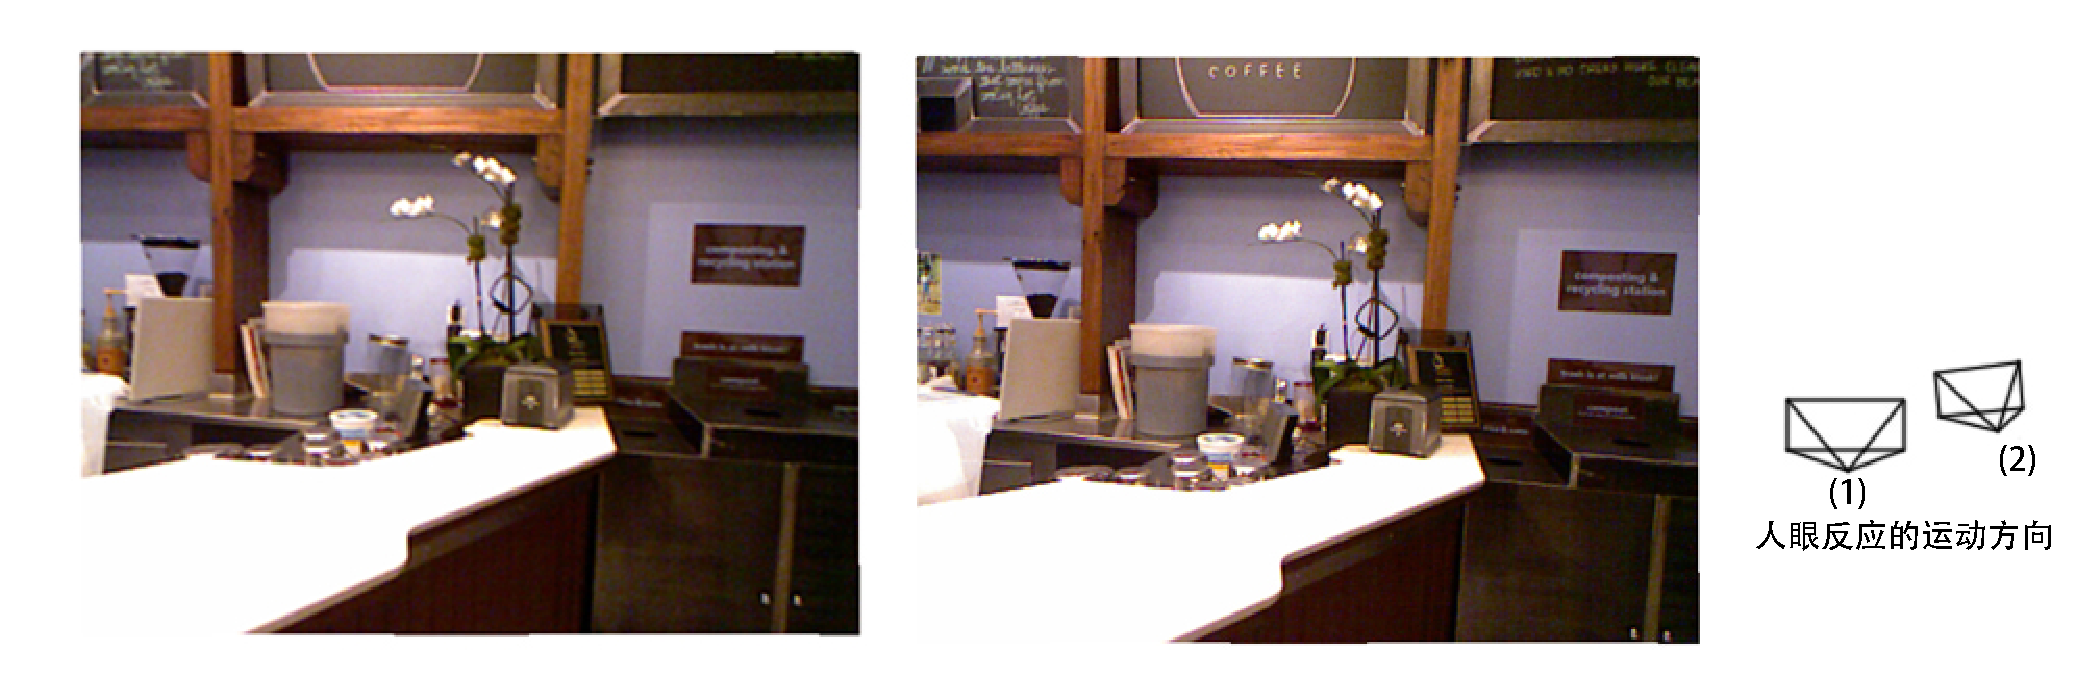
\includegraphics[width=1.0\textwidth]{./resources/whatIsSLAM/cameramotion.pdf}
    \caption{Camera motion can be inferred from two consecutive image frames. Images are from NYUD dataset.}
    \label{fig:cameramotion}
\end{figure}

But if we go a step further: can we determine how much the camera has rotated or translated, in units of degrees or centimeters? It is still difficult for us to give an quantitative answer. Because our intuition is not good at calculating numbers. But for a computer, movements have to be described with such numbers. So we will ask: how should a computer determine a camera's motion only based on images?

As mentioned earlier, in the field of computer vision, a task that seems natural to a human can be very challenging for a computer. Images are nothing but numerical matrices in computers. A computer has no idea what these matrices mean (this is the problem that machine learning is also trying to solve). In visual SLAM, we can only see blocks of pixels, knowing that they are the results of projections by spatial points onto the camera's imaging plane. In order to quantify a camera's movement, we must first \emph{understand the geometric relationship between a camera and the spatial points}.

Some background knowledge is needed to clarify this geometric relationship and the realization of VO methods. Here we only want to convey an intuitive concept. For now, you just need to take away that VO is able to estimate camera motions from images of adjacent frames and restore the 3D structures of the scene. It is named as an ``odometry'', because similar to an actual wheel odometry which only calculates the ego-motion at neighboring moments, and does not estimate a global map or a absolute pose. In this regard, VO is like a species with only a short memory.

Now, assuming that we have a visual odometry, we are able to estimate camera movements between every two successive frames. If we connect the adjacent movements, this constitutes the movement of the robot trajectory, and therefore addresses the positioning problem. On the other hand, we can calculate the 3D position for each pixel according to the camera position at each time step, and they will form an map. Up to here, it seems with an VO, the SLAM problem is already solved. Or, is it?

Visual odometry is indeed an key technology to solving visual SLAM problem. We will be spending a great part to explain it in details. However, using only a VO to estimate trajectories will inevitably cause \emph{accumulative drift}. This is due to the fact that the visual odometry (in the simplest case) only estimates the movement between two frames. We know that each estimate is accompanied by a certain error, and because the way odometry works, errors from previous moments will be carried forward to the following moments, resulting in inaccurate estimation after a period of time (see Fig.~\ref{fig:loopclosure}). For example, the robot first turns left 90$^\circ$ and then turns right 90$^\circ$. Due to error, we estimate the first 90$^\circ$ as 89$^\circ$, which is possible to happen in real-world applications. Then we will be embarrassed to find that after the right turn, the estimated position of the robot will not return to the origin. What's worse, even the following estimates are perfectly estimated, they will always be carrying this 1$^\circ$ error compared to the true trajectory.

\begin{figure}
    \centering
    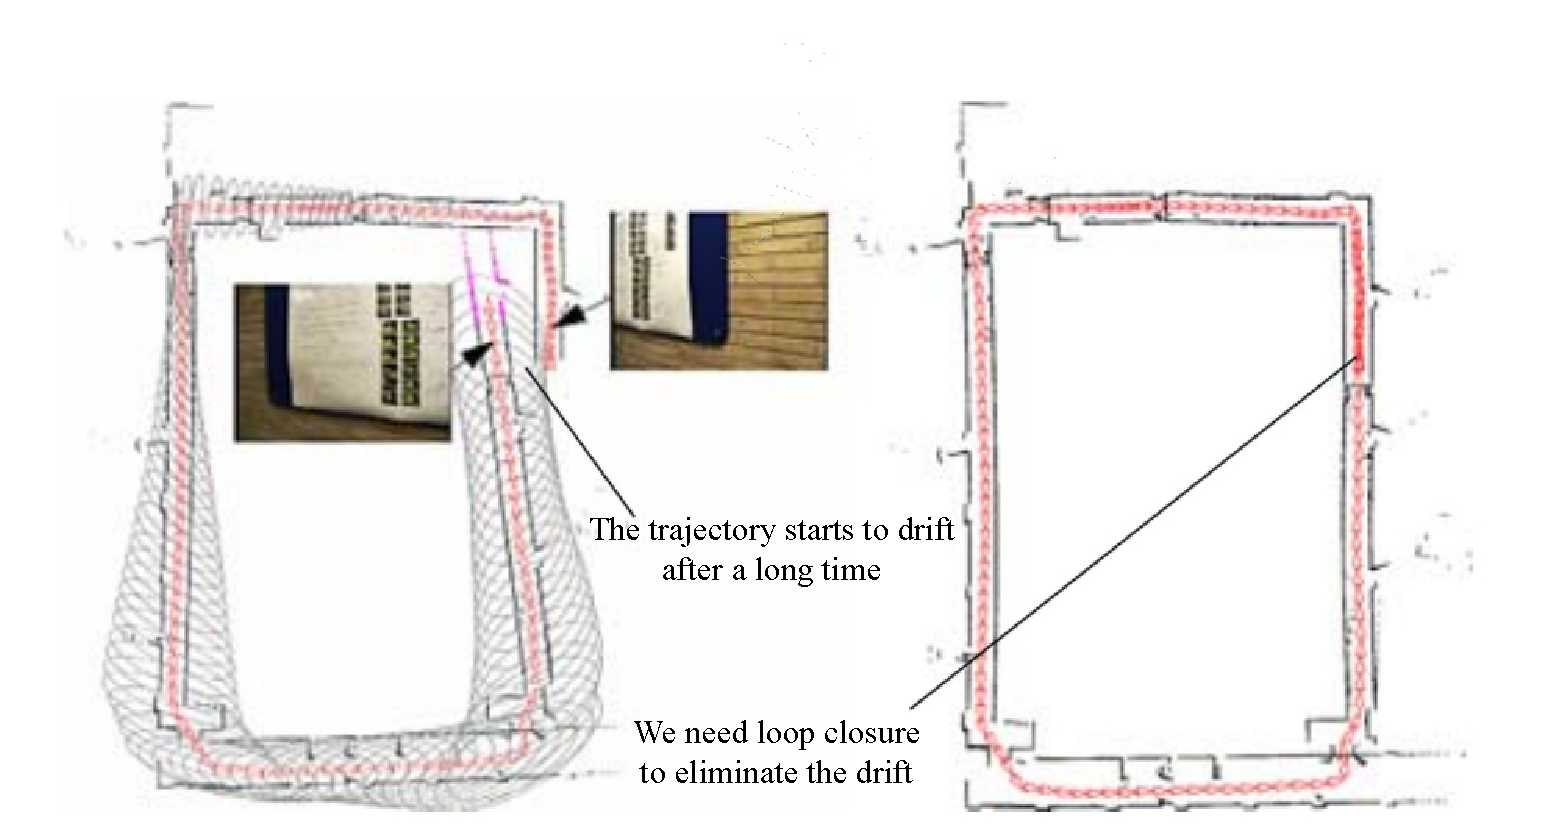
\includegraphics[width=1.0\textwidth]{./resources/whatIsSLAM/loopclosure.pdf}
    \caption{Drift will be accumulated if we only have a relative motion estimation.}
    \label{fig:loopclosure}
\end{figure}

The accumulated drift will make us unable to build a consistent map. A straight corridor may oblique, and a 90$^\circ$ angle may be crooked - this is really an unbearable matter! In order to solve the drifting problem, we also need other two components: the \emph{back-end optimization} \footnote{It is usually known as the back end. Since it is often implemented by optimization so we use the term back-end optimization.} and \emph{loop closing}. Loop closing is responsible for detecting whether the robot returns to its previous position, while the back-end optimization corrects the shape of the entire trajectory based on this information.


\subsubsection{ Back-end Optimization}
Generally speaking, the back-end optimization mainly refers to the process of dealing with the \emph{noise} in SLAM systems. We wish that all the sensor data is accurate, but in reality, even the most expensive sensors still have certain amount of noise. Cheap sensors usually have larger measurement errors, while that of expensive ones may be small. Moreover, performance of many sensors are affected by changes in magnetic field, temperature, etc. Therefore, in addition to solving the problem of estimating camera movements from images, we also care about how much noise this estimation contains, how these noise is carried forward from the last time step to the next, and how confident we have on the current estimation. So the problem that back-end optimization solves can be summarized as: to estimate the state of the entire system from noisy input data and calculate how uncertain these estimations are. The state here includes both the robot's own trajectory and the environment map.

In contrast, the visual odometry part is usually referred to as the \emph{front end}. In a SLAM framework, the front end provides data to be optimized by the back end, as well as the initial values. Because the back end is responsible for the overall optimization, we only care about the data itself instead of where it comes from. In other words, we only have numbers and matricies in backend without those beatiful images. In visual SLAM, the front end is more relevant to \emph{computer vision} topics, such as image feature extraction and matching, while the backend is relevant to \emph{state estimation} research area.

Historically, the back-end optimization part has been equivalent to ``SLAM research'' for a long time. In the early days, SLAM problem was described as a state estimation problem, which is exactly what the back-end optimization tries to solve. In the earliest papers on SLAM, researchers at that time called it ``estimation of spatial uncertainty'' \cite{Smith1986, Smith1990}. Although sounds a little obscure, it does reflect the nature of the SLAM problem: \emph{the estimation of the uncertainty of the self-movement and the surrounding environment}. In order to solve the SLAM problem, we need state estimation theory to express the uncertainty of localization and map construction, and then use filters or nonlinear optimization to estimate the mean and uncertainty (covariance) of the states. The details of state estimation and non-linear optimization will be explained in chapter 6, 10 and 11.

\subsubsection{Loop Closing}
Loop Closing, also known as \emph{Loop Closure Detection}, is mainly to address the drifting problem of position estimation in SLAM. So how to solve it? Assuming that a robot has returned to its origin after a period of movement, but the estimated position does not return to the origin due to drift. How to correct it? Imagine that if there is some way to let the robot know that it has returned to the origin, then we can then ``pull'' the estimated locations to the origin to eliminate drifts, which is, exactly, called loop closing.

Loop closing has close relationship with both localization and map building. In fact, the main purpose of building a map is to enable a robot to know the places it has been to. In order to achieve loop closing, we need to let the robot has the ability to identify the scenes it has visited before. There are different alternatives to achieve this goal. For example, as we mentioned earlier, we can set a marker at where the robot starts, such as a QR code. If the sign was seen again, we know that the robot has returned to the origin. However, the marker is essentially an intrusive sensor which sets additional constraints to the application environment. We prefer the robot can use its non-intrusive sensors, e.g. the image itself, to complete this task. A possible approach would be to detect similarities between images. This is inspired by us humans. When we see two similar images, it is easy to identify that they are taken from the same place. If the loop closing is successful, accumulative error can be significantly reduced. Therefore, visual loop detection is essentially an algorithm for calculating similarities of images. Note that the loop closing problem also exists in laser based SLAM, but here the rich information contained in images can remarkably reduce the difficulty of making a correct loop detection.

After a loop is detected, we will tell the back-end optimization algorithm that, OK,  ``A and B are the same point''. Then, based on this new information, the trajectory and the map will be adjusted to match the loop detection result. In this way, if we have sufficient and reliable loop detection, we can eliminate cumulative errors, and get globally consistent trajectories and maps.

\subsubsection{Mapping}
Mapping means the process of building a map, whatever kind it is. A map (see Fig.~\ref{fig:mapping}) is a description of the environment, but the way of description is not fixed and depends on the actual application.

\begin{figure}
	\centering
	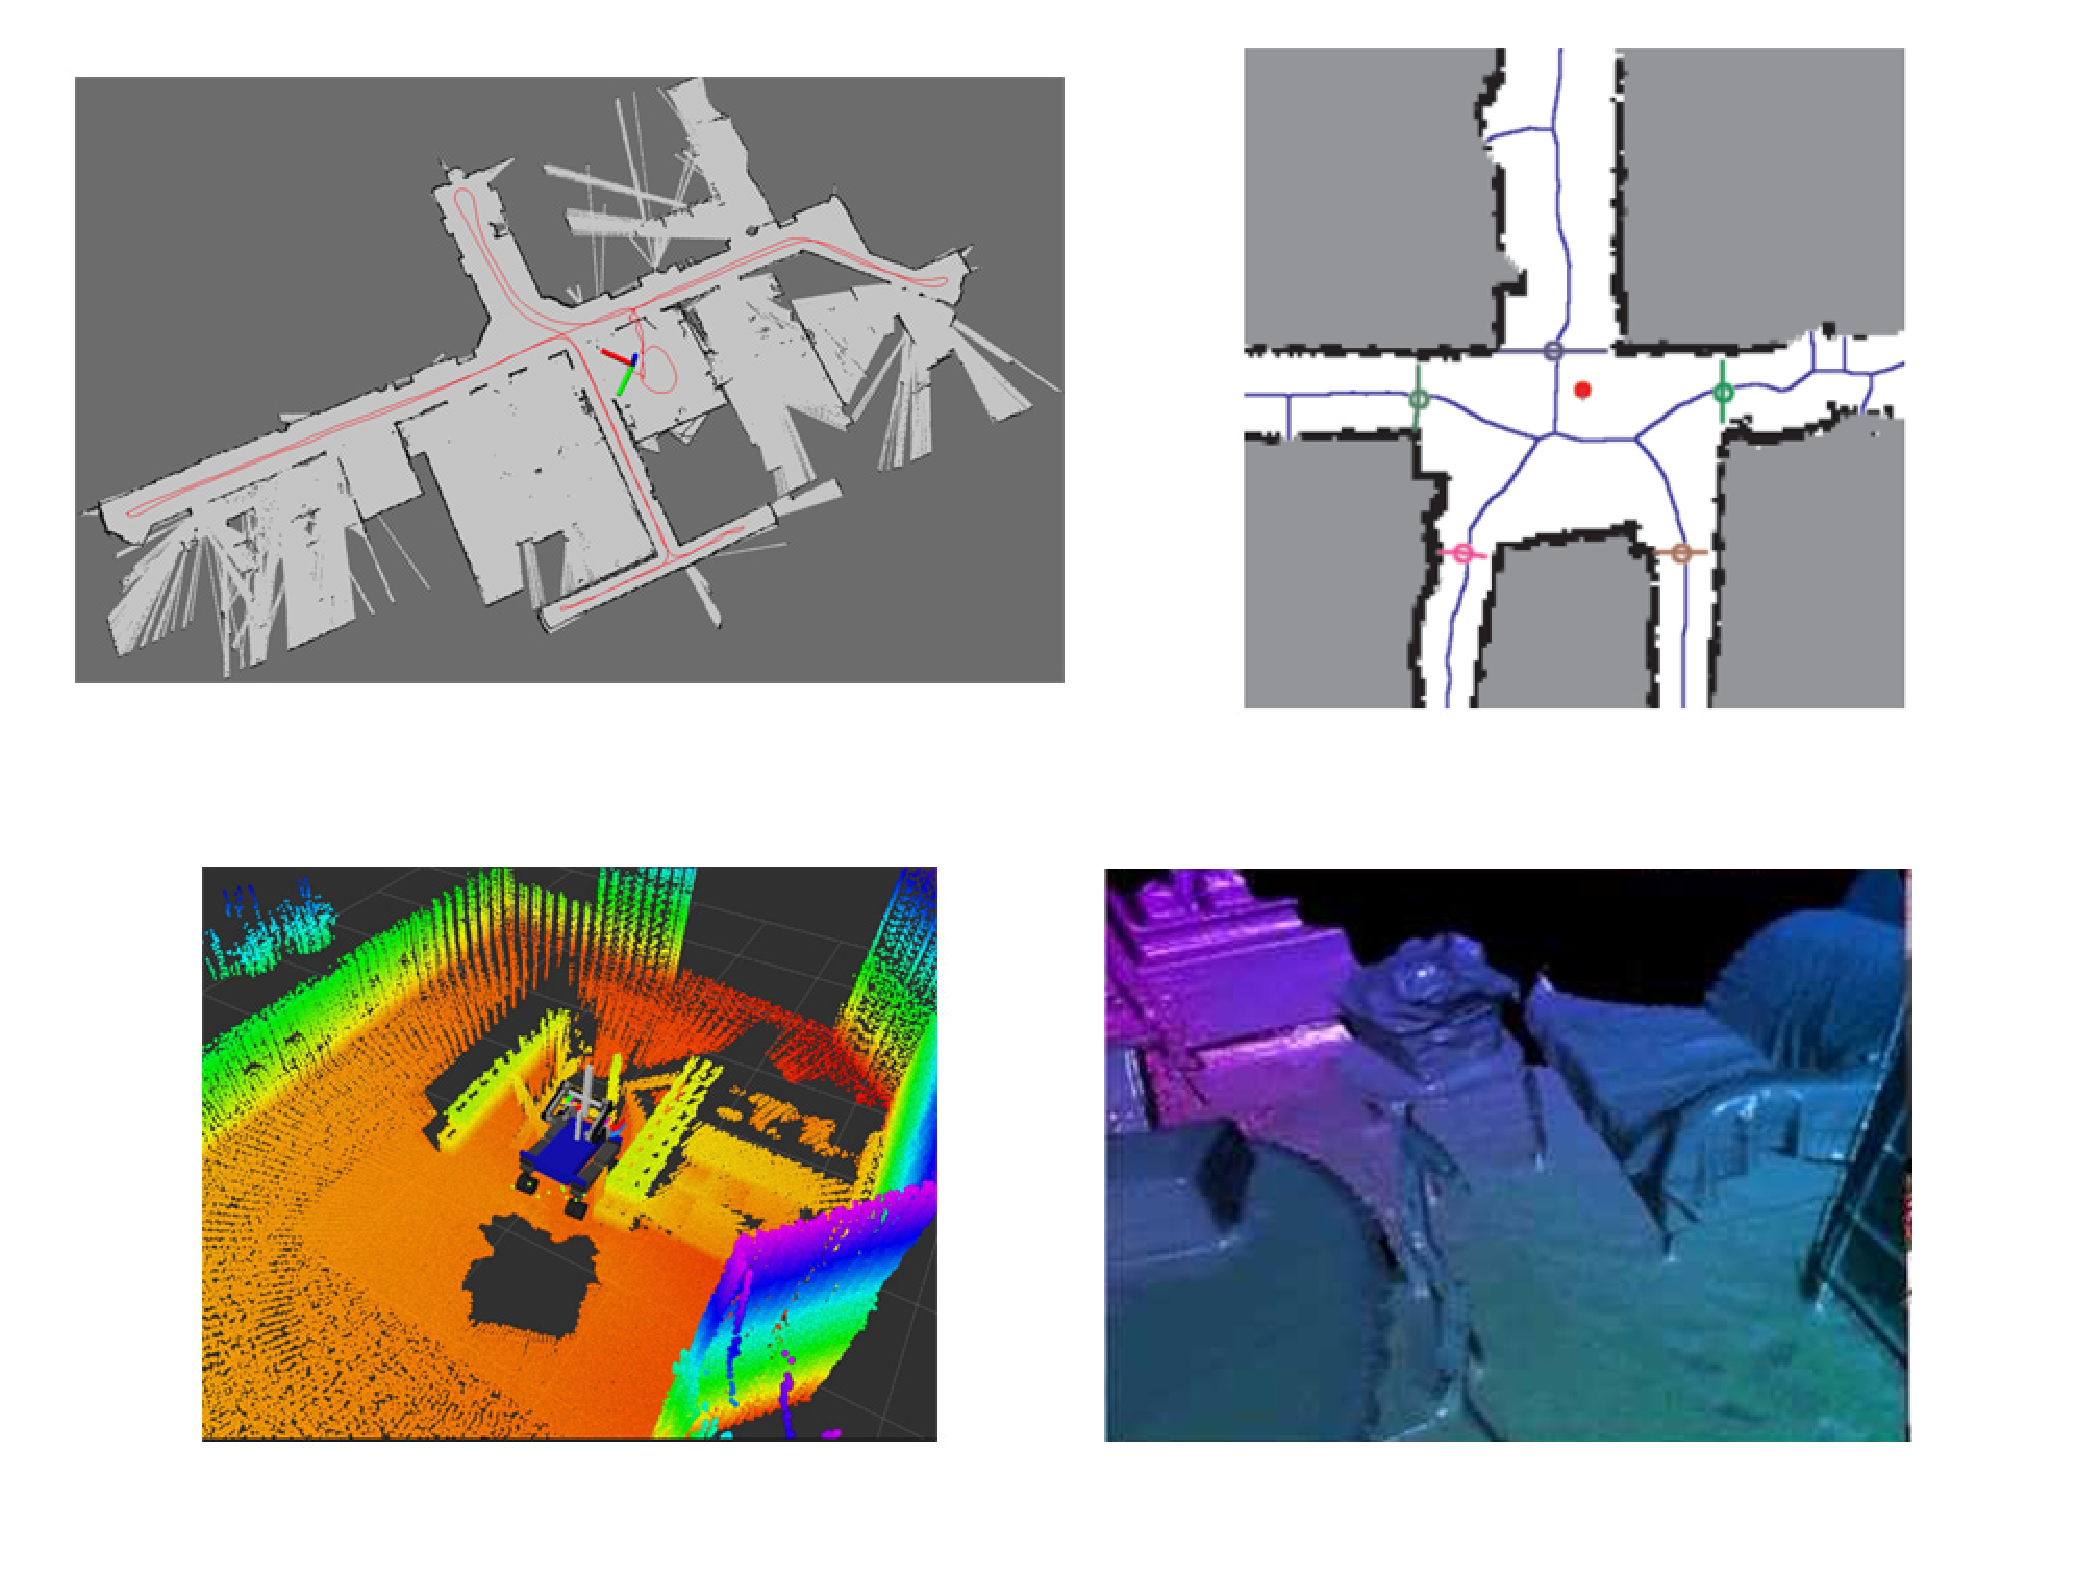
\includegraphics[width=1.0\textwidth]{./resources/whatIsSLAM/map.pdf}
	\caption{Different kinds of maps: 2D grid map, 2D topological map, 3D point clouds and 3D meshes.}
	\label{fig:mapping}
\end{figure}

Let's take the domestic cleaning robots as an example. Since they basically move on the ground, a two-dimensional map with marks for open areas and obstacles, built by a single line laser scanner, would be sufficient for navigation for them. And for a camera, we need at least a three-dimensional map for its 6 degrees of freedom movement. Sometimes, we want a smooth and beautiful reconstruction result, not just a set of points, but also with texture of triangular faces. And at other times, we do not care about the map, just need to know things like "point A and point B are connected, while point B and point C are not", which is a topological way to understand the environement. Sometimes maps may not even be needed, for instance, a level-3 autonomous driving car can make a lane-following driving only knowing its relative motion with the lanes.

For maps, we have various ideas and demands. So compared to the previously mentioned VO, loop closure detection and back-end optimization, map building does not have a certain algorithm. A collection of spatial points can be called a map, a beautiful 3D model is also a map, so is a picture of a city, a village, railways, and rivers. The form of the map depends on the application of SLAM. In general, they can be divided into to categories: \emph{metrical map} and \emph{topological map}.

\paragraph{Metric Map}
Metrical maps emphasize the exact metrical locations of the objects in maps. They are usually classified as either sparse or dense. Sparse metric maps store the scene into a compact form, and do not express all the objects. For example, we can construct a sparse map by selecting representative landmarks such as the lanes and traffic signs, and ignore other parts. In contrast, dense metrical maps focus on modeling all the things that are seen. For localization, sparse map would be enough, while for navigation, a dense map is usually needed (otherwise we may hit a wall between two landmarks). A dense map usually consists of a number of small pieces at a certain resolution. It can be small grids for 2D metric maps, or small voxels for 3D maps. For example, in a grid map, an grid may have three states: occupied, idle, and unknown, to express whether there is an object. When a spatial location is queried, the map can give the information about whether the location can be passed through. This type of maps can be used for a variety of navigation algorithms, such as A$^*$, D$^*$\footnote{ See \url{https://en.wikipedia.org/wiki/A*_search_algorithm}.}, etc., and thus attracts the attention of robotics researchers. But we can also see that all the grid status are store in the map, and thus being storage expensive. There are also some open issues in building a metrical map, for example, in large-scale metrical maps, a little bit of steering error may cause the walls of two rooms to overlap with each other, and thus making the map ineffective.

\paragraph{Topological Map}
Compared to the accurate metrical maps, topological maps emphasize the relationships among map elements. A topological map is a graph composed of nodes and edges, only considering the connectivity between nodes. For instance, we only care about that point A and point B are connected, regardless how we could travel from point A to point B. It relaxes the requirements on precise locations of a map by removing map details, and is therefore a more compact expression. However, topological maps are not good at representing maps with complex structures. Questions such as how to split a map to form nodes and edges, and how to use a topological map for navigation and path planning, are still open problems to be studied.

\section{Mathematical Formulation of SLAM Problems}
Through the previous introduction, readers should have gained an intuitive understanding of the modules in a SLAM system and the main functionality of each module. However, we cannot write runable programs only based on intuitive impressions. We want to rise it to a rational and rigorous level, that is, using mathematical symbols to formulate a SLAM process. We will be using variables and formulas, but please rest assured that we will try our best to keep it clear enough.

Assuming that our Little Carrot is moving in an unknown environment, carrying some sensors. How can this be described in mathematical language? First, since sensors usually collect data at different some time points, we are only concerned with the locations and map at these moments. This turns a continuous process into discrete time steps, say $1, \cdots, k$, at which data sampling happens. We use $\mathbf{x}$ to indicate positions of Little Carrot. So the positions at different time steps can be written as $\mathbf{x}_1,\cdots,\mathbf{x}_k$, which constitute the trajectory of Little Carrot. In terms of the map, we assume that the map is made up of a number of \emph{landmarks}, and at each time step, the sensors can see a part of the landmarks and record their observations. Assume there are total $N$ landmarks in the map, and we will use $\mathbf{y}_1, \cdots, \mathbf{y}_N$ to denote them.

With such a setting, the process that ``Little Carrot move in the environment with sensors'' basically has two parts: 

\begin{enumerate}
\item What is its \emph{motion}? We want to describe how $\mathbf{x}$ is changed from time step $k-1$ to $k$.
\item What are the sensor \emph{observations}? Assuming that the Little Carrot detects a certain landmark, say $\mathbf{y}_j$ at position $\mathbf{x}_k$, we need to describe this event in mathematical language.
\end{enumerate}

Let's first take a look at motion. Typically, we may send some motion message to the robots like ``turn 15 degree to left''. These messages or orders will be finally carried out by the controller, but probably in may different ways. Sometimes we control the position of robots, but acceleration or angular velocity would always be reasonable alternates. However, no matter what the controller is, we can use a universal and abstract mathematical model to describe it:
\begin{equation}
{\mathbf{x}_k} = f\left( {{\mathbf{x}_{k - 1}},{\mathbf{u}_k}, \mathbf{w}_k} \right),
\end{equation}
where $\mathbf{u}_k$ is the input orders, and $\mathbf{w}_k$ is noise. Note that we use a general $f(\cdot)$ to describe the process, instead of specifying the exact form of $f$. This allows the function to represent any motion input, rather than being limited to a particular one, and thus becoming a general equation. We call it the \emph{motion equation}.

The presence of noise turns this model into a stochastic model. In other words, even if we give the order like ``move forward one metes'', it does not mean that our robot really advances one meter. If all the instructions are accurate, there is no need to \emph{estimate} anything. In fact, the robot may only advance by, say, 0.9 meters, and at another moment, it moves by 1.1 meters. Thus, the noise during each movement is random. If we ignore this noise, the position determined only by the command may be a hundred miles away from the actual position after several minutes.

Corresponding to the motion equation, there is also a \emph{observation equation}. The observation equation describes the process that the Little Carrot sees a landmark point $\mathbf{y}_j$ at $\mathbf{x}_k$ and generates an observation data $\mathbf{z}_{k,j}$. Likewise, we will describe this relationship with an abstract function $h(\cdot)$:
\begin{equation}
{\mathbf{z}_{k,j}} = h\left( {{\mathbf{y}_j},{\mathbf{x}_k}, \mathbf{v}_{k,j} } \right),
\end{equation}
where $\mathbf{v}_{k,j}$ is the noise in this observation. Since there are various forms of observation sensors, the observed data $\mathbf{z}$ and the observation equation $h$ may also have many different forms.

%Readers may wonder that the function ![](http://latex.codecogs.com/gif.latex?f,h) we used do not seem to specify what the motion and observations exactly are. Besides, what are ![](http://latex.codecogs.com/gif.latex?\\mathbf{x}), ![](http://latex.codecogs.com/gif.latex?\\mathbf{y}), ![](http://latex.codecogs.com/gif.latex?\\mathbf{z}) here? In fact, according to the actual movement of Little Carrot and the type of sensor it carries, there are different ways for **parameterization**. What is parameterization then? For example, suppose the Little Carrot moves in a plane, then its pose (footnote: In this book, we use the word "pose" to refer to "position" plus "orientation".) is described by two position values and one angle, i.e. ![](http://latex.codecogs.com/gif.latex?\\mathbf{x}_k=[x,y,\theta]_k^\mathrm{T}). At the same time, the motion sensor can measure the amount of change in the position and angle of Little Carrot at any time step interval ![](http://latex.codecogs.com/gif.latex?\\mathbf{u}_k=[\\Delta{x},\\Delta{y},\\Delta\\theta]_k^\\mathrm{T}). Then, the motion equation can be specified as 
%
%![](http://latex.codecogs.com/gif.latex?{\\left[\\begin{array}{l}x\\\y\\\\\theta\\end{array}\\right]_k}={\\left[\\begin{array}{l}x\\\y\\\\\theta\\end{array}\\right]_{k-1}}+{\\left[\\begin{array}{l}\\Delta{x}\\\\\Delta{y}\\\\\Delta\\theta\\end{array}\\right]_k}+w_k)
%
%This is a simple linear relationship. However, not all of the sensors can directly measure the displacement and angle changes, so there are other forms of more complex equations of motion, then we may need to carry out dynamic analysis. On the observation equation, for example, a small radish carrying a two-dimensional laser sensor. We know that when a laser sensor observes a 2D punctuation, two quantities can be measured: the distance between the road sign and the radish body is $ r $ and the angle $$ \ phi $$. The observation data is $ \ bm {y} = [p_x, p_y] ^ \ mathrm {T} $ (for the sake of simplicity, omitting the subscript), the observation data is $ \ bm {z} = [r, \ phi] ^ \ Mathrm {T} $, then the observation equation is as follows:
% !Mode:: "TeX:UTF-8"
\chapter{3D Rigid Body Motion}

\begin{mdframed}
	\textbf{Goal of Study}
	\begin{enumerate}
		\item Understand the description of rigid body motion in three-dimensional space: rotation matrix, transformation matrix, quaternion and Euler angle.
		\item Understand the matrix and geometry module usage of the Eigen library.
	\end{enumerate}
\end{mdframed}

In the last lecture, we explained the framework and content of visual SLAM. This lecture will introduce one of the basic problems of visual SLAM: \textbf{ How to describe the motion of a rigid body in three-dimensional space?} Intuitively, we certainly know that this consists of one rotation plus one translation. Translation does not really have much problem, but the processing of rotation is a hassle. We will introduce the meaning of rotation matrices, quaternions, Euler angles, and how they are computed and transformed. In the practice section, we will introduce the linear algebra library Eigen. It provides a C++ matrix calculation, and its Geometry module also provides the structure described quaternion like rigid body motion. Eigen's optimization is perfect, but there are some special places to use it, we will leave it to the program.

\section{Rotation Matrix}
\label{sec:3.1}
\subsection{Point, Vector and Coordinate System}
The space in our daily life is three-dimensional, so we are born to be used to the movement of three-dimensional space. The three-dimensional space consists of three axes, so the position of one spatial point can be specified by three coordinates. However, we should now consider \textbf{rigid body} , which has not only its position, but also its own posture. The camera can also be viewed as a rigid body in three dimensions, so the position is where the camera is in space, and the attitude is the orientation of the camera. Combined, we can say, "The camera is in the space $ ( 0, 0 , 0 ) $ point, facing the front". But this natural language is cumbersome, and we prefer to describe it in a mathematical language.

We start with the most basic content: \textbf{points} and \textbf{vectors}. Points are the basic elements in space, no length, no volume. Connecting the two points forms a vector. A vector can be thought of as an arrow pointing from one point to another. We need to remind the reader that, please do not confuse the vector with its \textbf{coordinates}. A vector is one of the things in space, such as $ \mathbf{a}$ . Here $ \mathbf{a} $ does not need to be associated with several real numbers. Only when we specify a \textbf{coordinate system} in this three-dimensional space can we talk about the coordinates of the vector in this coordinate system, that is, find several real numbers corresponding to this vector.

With the knowledge of linear algebra, the coordinates of a point in 3D space can also be described by $ \mathbb{R}^3$. How to describe it? Suppose that in this linear space, we find a set of \textbf{base} \footnote{Just a reminder here, the base is a set of linearly independent vectors in the space, normally being orthognal and has unit-length.} $ (\mathbf{e}_1,\mathbf{e}_2,\mathbf{e}_3) $ , then, the arbitrary vector $ \mathbf{a} $ has a \textbf{coordinate} under this set of bases:

\begin{equation}
\mathbf{a} = \left[ {{\mathbf{e}_1},{\mathbf{e}_2},{\mathbf{e}_3}} \right]\left[ \begin{array}{l}
{a_1}\\
{a_2}\\
{a_3}
\end{array} \right] = {a_1}{\mathbf{e}_1} + {a_2}{\mathbf{e}_2} + {a_3}{\mathbf{e}_3}.
\end{equation}

Here $ (a_ 1 , a_ 2 , a_ 3 )^ \mathrm {T} $ is called $\mathbf {a}$'s coordinates \footnote {We use column vectors in this book which is same as most of the  mathematics books.}. The specific values of the coordinates are related to the vector itself, and also the selection of the bases. In $\mathbb{R}^3$, the coordinate system usually consists of 3 orthogonal coordinate axes (although it can also be non-orthogonal, it is rare in practice). For example, given $ \mathbf {x} $ and $ \mathbf {y} $ axis, the $ \mathbf {z} $ axis can be found using the right-hand (or left-hand) rule by $ \mathbf {x} \times  \mathbf {y} $. According to different definitions, the coordinate system is divided into left-handed and right-handed. The third axis of the left hand system is opposite to the right hand system. Most 3D libraries use right-handed (such as OpenGL, 3D Max, etc.), and some libraries use left-handed (such as Unity, Direct3D, etc.).

Based on basic linear algebra knowledge, we can talk about the operations between vectors/vectors, and vectors/numbers, such as scalar multiplication, vector addition, subtraction, inner product, outer product, and so on. Multiplication, addition and subtraction are fairly basic and intuitive. For example, the result of adding two vectors is to add their respective coordinates, subtraction, and so on. I won't go into details here. Internal and external products may be somewhat unfamiliar to the reader, and their calculations are given here. For $ \mathbf {a}, \mathbf {b} \in  \mathbb {R}^ 3 $ , in the usual sense \footnote {the inner product also has formal rules, but this book only discusses the usual inner product.} , the inner product of $\mathbf{a}, \mathbf{b}$ can be written as:

\begin{equation}
\mathbf{a} \cdot \mathbf{b} = { \mathbf{a}^\mathrm{T}}\mathbf{b} = \sum\limits_{i = 1}^3 {{a_i}{b_i}}  = \left| \mathbf{a} \right|\left| \mathbf{b} \right|\cos \left\langle {\mathbf{a},\mathbf{b}} \right\rangle ,
\end{equation}
where $ \left \langle { \mathbf {a}, \mathbf {b}} \right \rangle $ refers to the angle between the vector $ \mathbf {a}, \mathbf {b} $ . The inner product can also describe the projection relationship between vectors. The outer product is like this:

\begin{equation}
\label{eq:cross}
\mathbf{a} \times \mathbf{b} = \left\| {\begin{array}{*{20}{c}}
	\mathbf{e}_1 & \mathbf{e}_2 & \mathbf{e}_3 \\
	{{a_1}}&{{a_2}}&{{a_3}}\\
	{{b_1}}&{{b_2}}&{{b_3}}
	\end{array}} \right\| = \left[ \begin{array}{l}
{a_2}{b_3} - {a_3}{b_2}\\
{a_3}{b_1} - {a_1}{b_3}\\
{a_1}{b_2} - {a_2}{b_1}
\end{array} \right] = \left[ {\begin{array}{*{20}{c}}
	0&{ - {a_3}}&{{a_2}}\\
	{{a_3}}&0&{-{a_1}}\\  
	{-{a_2}}&{{a_1}}&0  
	\end{array}} \right] \mathbf{b} \buildrel \Delta \over = { \mathbf{a}^ \wedge } \mathbf{b}.
\end{equation}

The result of the outer product is a vector whose direction is perpendicular to the two vectors, and the length is $ \left | \mathbf{a} \right | \left | \mathbf{b} \right | \left \langle { \mathbf {a}, \mathbf {b}} \right \rangle  $, which is also the area of the quadrilateral of the two vectors. For the outer product operations, we introduce the $ ^ \wedge $ operator here, which means writing $ \mathbf{a} $ as a matrix. In fact, it is a \textbf {skew-symmetric matrix}\footnote{Skew-symmetric matrix means $ \mathbf{A} $ satisfies $ \mathbf{A}^ \mathrm{T}=- \mathbf{A}$. }. You can take $ ^ \wedge $ as an skew-symmetric symbol. It turns the outer product $ \mathbf{a} \times  \mathbf{b} $ into the multiplication of the matrix and the vector $ { \mathbf{a}^ \wedge } \mathbf{b} $ , which turns it into a linear operator. This symbol will be used frequently in the following sections, and this symbol is a one-to-one mapping, meaning that for any vector, it corresponds to a unique anti-symmetric matrix, and vice versa:

\begin{equation}
\mathbf{a}^\wedge = \left[ {\begin{array}{*{20}{c}}
	0&{-{a_3}}&{{a_2}}\\  
	{{a_3}}&0&{ - {a_1}}\\
	{ - {a_2}}&{{a_1}}&0
	\end{array}} \right].
\end{equation}

At the same time, note that the vector operations such as addition, subtraction, internal and external products, can be calculated even when we do not have their coordinates. For example, although the inner product can be expressed by the sum of the product products of the two vectors when we know the coordinates, it can also be calculated by the length and the angle even if their coordinates are unknown. Therefore, the inner product result of the two vectors is independent of the selection of the coordinate system.
% !Mode:: "TeX:UTF-8"
\chapter{Lie Group and Lie Algebra}
\label{cpt:4}
\begin{mdframed}
    \textbf{Main Goal}
    \begin{enumerate}
        \item Understand the concept of Lie group, Lie algebra, and their applications of $ \mathrm{SO}( 3 ), \mathrm{SE}( 3 ) $ and the corresponding Lie algebras.
        \item Understands the meaning of BCH formula.
        \item Learn the perturbation model on Lie algebra.
        \item Use Sophus to perform operations on Lie algebras.
    \end{enumerate}
\end{mdframed}

In the last lecture, we introduced the description of rigid body motion in the three-dimensional world, including the rotation matrix, rotation vector, Euler angle, quaternion and so on. We focus on the representation of rotation, but in SLAM we have to estimate and optimize them in addition to the representation. Because the pose is unknown in SLAM, we need to solve the problem of ``\textbf {which camera pose best matches the current observation}''. A typical way is to build it into an optimization problem, solving the optimal $ \mathbf{R}, \mathbf{t}$ , and minimizing the error.

As mentioned before, the rotation matrix itself is constrained (orthogonal and the determinant is 1). When used as optimization variables, it introduces additional constraints on matrices that makes optimization difficult. Through the transformation relationship between Lie group and Lie algebra, we are able to turn the pose estimation into an unconstrained optimization problem and simplify the solution. Considering that the reader may not have the basic knowledge of Lie Group and Lie algebra, we will start with the most basic knowledge.

\newpage
\section{Basics of Lie Group and Lie Algebra}
In the last lecture, we introduced the definition of the rotation matrix and the transformation matrix. At the time, we said that the three-dimensional rotation matrix constitutes \textbf{special orthogonal group} $\mathrm{SO}(3)$, and the transformation matrix constitutes \textbf{special Euclidean group} $\mathrm{SE}(3) $. They are written like this:
\begin{equation}
\mathrm{SO}(3) = \{ \mathbf{R} \in \mathbb{R}^{3 \times 3} | \mathbf{RR}^\mathrm{T} = \mathbf{I}, \ Det(\mathbf{R})=1 \}.
\end{equation}
\begin{equation}
\mathrm{SE}(3) = \left\{ \mathbf{T} = \left[ {\begin{array}{*{20}{c}}
    \mathbf{R} & \mathbf{t} \\
    {{\mathbf{0}^\mathrm{T}}} & 1
    \end{array}} \right]
\in \mathbb{R}^{4 \times 4} | \mathbf{R} \in \mathrm{SO}(3), \mathbf{t} \in \mathbb{R}^3\right\}.
\end{equation}

However, at the time we did not explain the meaning of \textbf{group} in detail. Readers should note that both of the rotation matrix and the transformation matrix \textbf{are not closed to addition}. In other words, for any two rotation matrices $\mathbf{R}_1, \mathbf{R}_2$, according to the definition, their addition is no longer a rotation matrix:
\begin{equation}
\mathbf{R}_1 + \mathbf{R}_2 \notin \mathrm{SO}(3), \quad \mathbf{T}_1 + \mathbf{T}_2 \notin \mathrm{SE}(3).
\end{equation}
You can also say that the two matrices do not have a well-defined addition operator, or the matrix addition is not closed in these two sets. We find they have only one closed operation: the multiplication:
\begin{equation}
\mathbf{R}_1 \mathbf{R}_2 \in \mathrm{SO}(3), \quad \mathbf{T}_1 \mathbf{T}_2 \in \mathrm{SE}(3).
\end{equation}
We know that the matrix multiplication corresponds to the composition of two rotations or transformations. For a set that only has one ``well-defined'' operation, we call it a \textbf{group}.

\subsection{Group}
For the next contents we need to talk about a little bit abstract algebra. I think this is a necessary condition for discussing Lie Group and Lie Algebra, but in fact, except for the students of mathematics and physics, most of the students will not have this knowledge in undergraduate classes. So let's look at some basic concepts first.

A group is an algebraic structure of \textbf{a collection} plus \textbf{an operation}. We denote the collection as $A$ and the operation as $\cdot$, then the group can be denoted as $G=(A,\cdot)$. We say $G$ is a \textbf{group} if the operation satisfies the following conditions:

\begin{enumerate}
    \item { {Closure}}: $ \  \forall a_1, a_2 \in A, \  a_1 \cdot a_2 \in A$.
    \item { {Combination}}: $ \  \forall a_1, a_2, a_3 \in A, \  (a_1 \cdot a_2) \cdot a_3 = a_1 \cdot ( a_2 \cdot a_3) $.
    \item { {Unit element}}: $ \  \exists a_0 \in A, \  \mathrm{s.t.} \ \forall a \in A, \  a_0 \cdot a = a \cdot a_0 = a $.
    \item { {Inverse element}}: $ \  \forall a \in A, \  \exists a^{-1} \in A, \  st \  a \cdot a^{-1} = a_0 $.
\end{enumerate}

It is easy to verify that the rotation matrix set with the normal matrix multiplication form a group, and the same for transformation matrix with matrix multiplication, so they can be called as rotation matrix group and transformation matrix group. Other common groups include the addition of integers $(\mathbb{Z}, +)$, the rational numbers with multiplication after removing 0 $(\mathbb{Q}\backslash 0, \cdot )$, etc. Common groups in the matrix are:

\begin{itemize}
    \item {General Linear group $\mathrm{GL}(n)$}. The invertible matrix of $n \times n$ with matrix multiplication.
    \item {Special Orthogonal Group $\mathrm{SO}(n)$}. Or the rotation matrix group, where $\mathrm{SO}(2)$ and $\mathrm{SO}(3) $ is the most common.
    \item {Special Euclidean group $\mathrm{SE}(n)$}. Or the $n$ dimensional transformation described earlier, such as $\mathrm{SE}(2)$ and $\ Mathrm{SE}(3)$.
\end{itemize}

The group structure guarantees that the operations on the group have very good properties, and the \textbf{group theory} is the theory that studies the various structures and properties of the groups. Readers interested in group theory can refer to any of the modern algebra books. \textbf{Lie Group} refers to a group with continuous (smooth) properties. Discrete groups like the integer group $\mathbb{Z}$ have no continuous properties, so they are not Lie groups. And obviously, $\mathrm{SO}(n)$ and $\mathrm{SE}(n)$ are continuous in real space because we can intuitively imagine that a rigid body moving continuously in space, so they are all Lie Groups. Since $\mathrm{SO}(3)$ and $\mathrm{SE}(3)$ are especially important for camera pose estimation, we mainly discuss these two Lie groups. However, strictly discussing the concepts of ``continuous'' and ``smooth'' requires knowledge of analysis and topology, but we are not mathematics books, so only some important conclusions directly related to SLAM are introduced. If the reader is interested in the theoretical nature of Lie Groups, please refer to the special books like \cite{Varadarajan2013}.

Normally we have two ways to introduce the Lie Groups or Lie Algebras. The first is to directly introduce Lie group and Lie algebra, and then tell the reader that each Lie group corresponds to a Lie algebra, but in this case, the reader will think that Lie algebra seems to be a symbol that jumps out with no reason, and does not know its physical meaning. So, I am going to take a little time to draw the Lie algebra from the rotation matrix, similar to the practice of \cite{Ma2012}. Let's start with the simpler $\mathrm{SO}(3)$, leading to the Lie algebra $\mathfrak{so}(3)$ above $\mathrm{SO}(3)$.

\subsection{Introduction of the Lie Algebra}
Consider an arbitrary rotation matrix $\mathbf{R}$, we know that it satisfies:
\begin{equation}
\mathbf{R} \mathbf{R}^\mathrm{T}=\mathbf{I}.
\end{equation}
Now, we say that $\mathbf{R}$ is the rotation of a camera that changes continuously over time, which is a function of time: $\mathbf{R}(t)$. Since it is still a rotation matrix, we have
\[
\mathbf{R}(t) \mathbf{R}(t) ^T = \mathbf{I}.
\]
Deriving time on both sides of the equation yields (we use $\dot{\mathbf{R}}$ to represent the derivative of $\mathbf{R}$ on time $t$, just like many control books):
\[
\dot{\mathbf{R}} (t) \mathbf{R} {(t)^\mathrm{T}} + \mathbf{R} (t) \dot{\mathbf{R}} {(t) ^\mathrm{T}} = 0.
\]
Put the second item to right:
\begin{equation}
\dot{\mathbf{R}} (t) \mathbf{R} {(t)^\mathrm{T}} = - \left( \dot{\mathbf{R}} (t) \mathbf{R} {(t)^\mathrm{T}} \right)^\mathrm{T} .
\end{equation}

It can be seen that $\dot{\mathbf{R}} (t) \mathbf{R} {(t)^\mathrm{T}}$ is a \textbf{skew-symmetric} matrix. Recall that we introduced the $^\wedge$ symbol when we mention about the cross product in \eqref{eq:cross}, which turns a vector into an skew-symmetric matrix. Similarly, for any skew-symmetric matrix, we can also find a unique vector corresponding to it. Let this operation be represented by the symbol $^{\vee}$:
\begin{equation}
{\mathbf{a}^ \wedge } = \mathbf{A} = \left[ {\begin{array}{*{20}{c}}
    0&{ - {a_3}}&{{a_2}}\\
    {{a_3}}&0&{ - {a_1}}\\
    { - {a_2}}&{{a_1}}&0
    \end{array}} \right], \quad
{ \mathbf{A}^ \vee } = \mathbf{a}.
\end{equation}

So, since $\dot{\mathbf{R}} (t) \mathbf{R} {(t)^\mathrm{T}}$ is an skew-symmetric matrix, we can find a three-dimensional vector $\boldsymbol{\phi} (t) \in \mathbb{R}^3$ corresponds to it:
\[
\dot{\mathbf{R}} (t) \mathbf{R}(t)^\mathrm{T} = \boldsymbol{\phi} (t) ^ {\wedge}.
\]

Right multiply with $\mathbf{R}(t)$ on both sides, since $\mathbf{R}$ is an orthogonal matrix, we have:
\begin{equation}
\label{eq:dR}
\dot{\mathbf{R}} (t) = \boldsymbol{\phi} (t)^{\wedge} \mathbf{R}(t) =
\left[ {\begin{array}{*{20}{c}}
    0&{ - {\phi _3}}&{{\phi _2}}\\
    {{\phi _3}}&0&{ - {\phi _1}}\\
    { - {\phi _2}}&{{\phi _1}}&0
    \end{array}} \right] \mathbf{R} (t).
\end{equation}

It can be seen that we can take the time derivative of a ration matrix just by multiplying a $\boldsymbol{\phi}^\wedge (t)$ matrix on the left. Consider at time $t_0=0$, and the rotation matrix is $\mathbf{R}(0) = \mathbf{I}$. According to the derivative definition, $\mathbf{R}(t)$ can be used to perform a first-order Taylor expansion around $t=0$:
\begin{equation}
\begin{aligned}
\mathbf{R} \left( t \right) & \approx \mathbf{R} \left( t_0 \right) + \dot {\mathbf{R}} \left( {{t_0}} \right)\left ( {t - {t_0}} \right)\\
&= \mathbf{I} + \boldsymbol{\phi} {\left( {{t_0}} \right)^ \wedge } \left( t \right).
\end{aligned}
\end{equation}

We see that $\boldsymbol{\phi}$ reflects the derivative of $\mathbf{R}$, so it is called the \textbf{Tangent Space} near the origin of $\mathrm{SO}(3)$. Also, if time $t$ is close to $t_0$, we assume $\boldsymbol{\phi}(t)$ to close to be a constant $\boldsymbol{\phi}(t_0) = \boldsymbol{\phi}_0$. Then according to the formula \eqref{eq:dR}, we have:
\[
\dot{\mathbf{R}} (t) = \boldsymbol{\phi} (t_0) ^ {\wedge} \mathbf{R}(t) \approx \boldsymbol{\phi}_0^ {\wedge} \mathbf {R}(t).
\]

The above formula is a differential equation for $\mathbf{R}$, and with the initial value $\mathbf{R}(0) = \mathbf{I}$, we have solution like:
\begin{equation}
\label{eq:so3ode}
\mathbf{R}(t) = \exp \left( \boldsymbol{\phi}_0^\wedge t \right).
\end{equation}

The reader can verify that the above equation holds for both the differential equation and the initial value. This means that around $t = 0$, the rotation matrix can be calculated from $\exp \left( \boldsymbol{\phi}_0^\wedge t \right)$\footnote{At this point we have not explained what this $\exp$ means and how it works. We will talk about its definition and calculation process right after this section. }. We see that the rotation matrix $\mathbf{R}$ is associated with another skew-symmetric matrix $\boldsymbol{\phi}_0^\wedge t$ through an exponential relationship. But what is the exponential of a matrix? Here we have two questions that need to be clarified:

\begin{enumerate}
    \item Given $\mathbf{R}$ at a certain moment, we can find a $\boldsymbol{\phi}$ that describes the local derivative relationship of $\mathbf{R}$. How are they correlated with each other? We will say that $\boldsymbol{\phi}$ corresponds to the Lie algebra $\mathfrak{so}(3)$ on $\mathrm{SO}(3)$;
    \item Second, when a vector $\boldsymbol{\phi}$ is given, how is $\exp (\boldsymbol{\phi} ^\wedge )$ calculated? Conversely, given $\mathbf{R}$, is there an opposite operation to calculate $\boldsymbol{\phi}$? In fact, this is the exponential/logarithmic mapping between Lie group and Lie algebra.
\end{enumerate}

Let's solve these two problems below.

\subsection{The Definition of Lie Algebra}
Now let's give the strict definition of Lie Algebra. Each Lie group has a Lie algebra corresponding to it. Lie algebra describes the local structure of the Lie group around it origin point, or in other words, is the tangent space. The general definition of Lie algebra is listed as follows:

A Lie algebra consists of a set $\mathbb{V}$, a scalar field $\mathbb{F}$, and a binary operation $[,]$. If they satisfy the following properties, then $(\mathbb{V}, \mathbb{F}, [,])$ is a Lie algebra, denoted as $\mathfrak{g}$.

\begin{enumerate}
    \item Closure.  $\forall \mathbf{X}, \mathbf{Y} \in \mathbb{V}, [\mathbf{X}, \mathbf{Y}] \in \mathbb{V}$.
    \item Bilinear. $\forall \mathbf{X},\mathbf{Y},\mathbf{Z} \in \mathbb{V}, a,b \in \mathbb{F }, $ we have:
    \[
    [a\mathbf{X}+b\mathbf{Y}, \mathbf{Z}] = a[\mathbf{X}, \mathbf{Z}] + b [ \mathbf{Y}, \mathbf{Z} ], \quad [\mathbf{Z}, a \mathbf{X}+b\mathbf{Y}] = a [\mathbf{Z}, \mathbf{X} ]+ b [\mathbf{Z},\mathbf{Y}] .
    \]
    \item Reflexive \footnote{ Reflexive means that an element operates with itself results in zero. } $\forall \mathbf{X} \in \mathbb{V}, [\mathbf{X},\mathbf{X}] = \mathbf{0}$.
    \item Jacobi equation. $\forall \mathbf{X},\mathbf{Y},\mathbf{Z} \in \mathbb{V}, [\mathbf{X}, [ \mathbf{Y},\mathbf{Z}] ] + [\mathbf{Z}, [\mathbf{X},\mathbf{Y}] ] + [\mathbf{Y}, [\mathbf{Z}, \mathbf{X}]] =\mathbf{0}$.
\end{enumerate}
The binary operation $[,]$ is called \textbf{Lie brackets}. On the first glance, we require a lot of properties about the operator of Lie bracket.  Compared to the simpler binary operations in the group, the Lie bracket expresses the difference between the two elements. It does not require a combination law, but requires the element and itself to be zero after the brackets. As an example, the cross product $\times$ defined on the 3D vector $\mathbb{R}^3$ is a kind of Lie bracket, so $\mathfrak{g} = (\mathbb{R}^3, \mathbb{R}, \times)$ constitutes a Lie algebra. The reader can try to substitute the cross product into the above four properties to verify the above conclusion.

\subsection{Lie Algebra $\mathfrak{so}(3)$}
The previously mentioned $\boldsymbol{\phi}$ is actually a kind of Lie algebra. The Lie algebra corresponding to $\mathrm{SO}(3)$ is a vector defined on $\mathbb{R}^3$, which we will denote as $\boldsymbol{\phi}$. According to the previous derivation, each $\boldsymbol{\phi}$ can generate an skew-symmetric matrix:
\begin{equation}
\label{eq:phi}
\boldsymbol{\varPhi} = \boldsymbol{\phi}^{\wedge} = \left[ {\begin{array}{*{20}{c}}
    0&{ - {\phi _3}}&{{\phi _2}}\\
    {{\phi _3}}&0&{ - {\phi _1}}\\
    { - {\phi _2}}&{{\phi _1}}&0
    \end{array}} \right] \in \mathbb{R}^{3 \times 3}.
\end{equation}

Under this definition, the two vectors $\boldsymbol{\phi}_1, \boldsymbol{\phi}_2$'s Lie brackets are:
\begin{equation}
[\boldsymbol{\phi}_1, \boldsymbol{\phi}_2] = \left( \bm{ \varPhi }_1 \bm{ \varPhi }_2 - \bm{ \varPhi }_2 \bm{ \varPhi }_1 \right)^\vee.
\end{equation}

The reader can verify that the Lie brackets under this definition satisfy the above properties. Since the vector $\boldsymbol{\phi}$ is one-to-one with the skew-symmetric matrix, we say the elements of $\mathfrak{so}(3)$ are three-dimensional vectors or three-dimensional skew-symmetric matrices, without any ambiguity:
\begin{equation}
\mathfrak{so}(3) = \left\{ \boldsymbol{\phi} \in \mathbb{R}^3 \ \text{or}\  \boldsymbol{\varPhi} = \boldsymbol{\phi^\wedge} \in \mathbb{ R}^{3 \times 3} \right\}.
\end{equation}
Some books also use the symbol $\widehat{\boldsymbol{\phi}}$ to represent $\boldsymbol{\phi}^\wedge$, but the meaning is the same. At this point, we have made it clear about the contents of $\mathfrak{so}(3)$. They are just a set of \textbf{3D vectors} which can be used to express the derivative of the rotation matrix. Its relationship to $\mathrm{SO}(3)$ is given by the exponential map:
\begin{equation}
\bm{R} = \exp ( \boldsymbol{\phi}^\wedge ).
\end{equation}
The exponential map will be introduced later. Since we have introduced $\mathfrak{so}(3)$, we will first look at the corresponding Lie algebra on $\mathrm{SE}(3)$.

\subsection{Lie Algebra $\mathfrak{se}(3)$}
For $\mathrm{SE}(3)$, it also has a corresponding Lie algebra $\mathfrak{se}(3)$. To save space, I won't start by taking time derivatives. Similar to $\mathfrak{so}(3)$, $\mathfrak{se}(3)$ is located in the $\mathbb{R}^6$ space:
\begin{equation}
\mathfrak{se}(3) = \left\{ { \boldsymbol{\xi} = \left[ \begin{array}{l}
    \boldsymbol{\rho} \\
    \boldsymbol{\phi}
    \end{array} \right]
    \in { \mathbb{R}^6} ,
    \boldsymbol{\rho} \in { \mathbb{R}^3}, \boldsymbol{\phi} \in \mathfrak{so} \left( 3 \right),{ \boldsymbol{\xi} ^ \wedge } = \left[ {\begin{array}{*{20}{c}}
        {{ \boldsymbol{\phi} ^ \wedge }}& \boldsymbol{\rho} \\
        {{\bm{0}^\mathrm{T}}}&0
        \end{array}} \right] \in { \mathbb{R}^{4 \times 4}}} \right\}.
\end{equation}
We write each $\mathfrak{se}(3)$ element as $\boldsymbol{\xi}$, which is a six-dimensional vector. The first three dimensions are ``translation part'' (but keep in mind that the meaning is \textbf{different} from the translation in the transformation matrix, we will see later), which is denoted as $\boldsymbol{\rho}$; after the three-dimensional rotation, there is a $\boldsymbol{\phi}$, which is essentially a $\mathfrak{so}(3)$ element\footnote{Please note that in some books the authors may put the rotation in front and the translation in the back, which has no significant difference.}. At the same time, we extended the meaning of the $^\wedge$ symbol. In $\mathfrak{se}(3)$, a six-dimensional vector is also converted to a four-dimensional matrix using the $^\wedge$ symbol, but no longer a skew-symmetric one:
\begin{equation}
{ \boldsymbol{\xi} ^ \wedge } = \left[ {\begin{array}{*{20}{c}}
    {{ \boldsymbol{\phi} ^ \wedge }}& \boldsymbol{\rho} \\
    {{\bm{0}^\mathrm{T}}}&0
    \end{array}} \right] \in { \mathbb{R}^{4 \times 4}}.
\end{equation}

We still use the $^\wedge$ and $^\vee$ symbols to refer to the relationship from ``vector to matrix'' and ``matrix to vector'' to maintain consistency with $\mathfrak{so}(3)$. They are still one-to-one correspondence. The readers can simply take $\mathfrak{se}(3)$ as a ``vector consisting of a translation plus a $\mathfrak{so}(3)$ element'' (although $\boldsymbol{\rho} $ is not the direct translation). Similarly, the Lie algebra $\mathfrak{se}(3)$ also has a Lie bracket similar to $\mathfrak{so}(3)$:
\begin{equation}
[ \boldsymbol{\xi}_1, \boldsymbol{\xi}_2 ] = \left( \boldsymbol{\xi}_1^\wedge \boldsymbol{\xi}_2^\wedge -\boldsymbol{\xi}_2^ \wedge \boldsymbol{\xi}_1^\wedge \right) ^\vee.
\end{equation}

The reader can verify that it satisfies the definition of Lie algebra (I'll leave it as an exercise). So far we have seen two important Lie algebras $\mathfrak{so}(3)$ and $\mathfrak{se}(3)$.
% !Mode:: "TeX:UTF-8"
\chapter{Cameras and Images}
\label{cpt:5}
\begin{mdframed}  
	\textbf{Goal of Study}
	\begin{enumerate}[labelindent=0em,leftmargin=1.5em]
		\item Learn the models of the pinhole camera, intrinsics, extrinsics, and distortion. 
		\item Learn how to project a spatial point into image planes. 
		\item Learn the basic image process in OpenCV. 
	\end{enumerate}
\end{mdframed} 

In the previous two lectures, we introduced how to express and optimize the robot's 6 DoF pose and partially explained the meaning of the variables and the equations of motion and observation in SLAM. This chapter will discuss ``How robots observe the outside world'', which belongs to the observation equation. In the camera-based visual SLAM, the observation mainly refers to the process of image projection.

We have seen a lot of photos in real life. A photo consists of millions of pixels in the computer, recording information about color or brightness. We will see a bundle of light reflected or emitted by an object in the three-dimensional world pass through the camera's optical center and is projected onto the camera's imaging plane. After the camera's light sensor receives the light, it produces a measurement, and we get the pixels, which form the photo we see. Can this process be described by mathematical equations? This lecture will first discuss the camera model, explain how the projection relationship is described, and the internal parameters in this projection process. At the same time, we will also give a brief introduction to the stereo and RGB-D cameras. Then, we introduce the basic operations of 2D images in OpenCV. Finally, an experiment of point cloud stitching is demonstrated to show the meaning of intrinsic and extrinsic parameters.

\newpage
\includepdf{resources/other/ch5.pdf}
\newpage
\section{Pinhole Camera Models}
The process of projecting a 3D point (in meters) to a 2D image plane (in pixels) can be described by a geometric model. Actually, several models describe this, the simplest of which is called the pinhole model. We will start with this pinhole projection. At the same time, due to the presence of the lens on the camera lens, \textit{distortion} is generated during the projection. Therefore, we will use the pinhole model plus a distortion model to describe the entire projection process.

\subsection{Pinhole Camera Geometry}
Most of us have seen the candle projection experiment in the physics class of high school: a lit candle is placed in front of a dark box, and the light of the candle is projected through a small hole in the dark box on the rear plane. Then an inverted candle image is formed on this plane. In this process, the small hole can project a candle in a three-dimensional world onto a two-dimensional imaging plane. For the same reason, we can use this simple model to explain the camera's imaging process, as shown in \autoref{fig:cameraModel}.

\begin{figure}[!ht]
	\centering
	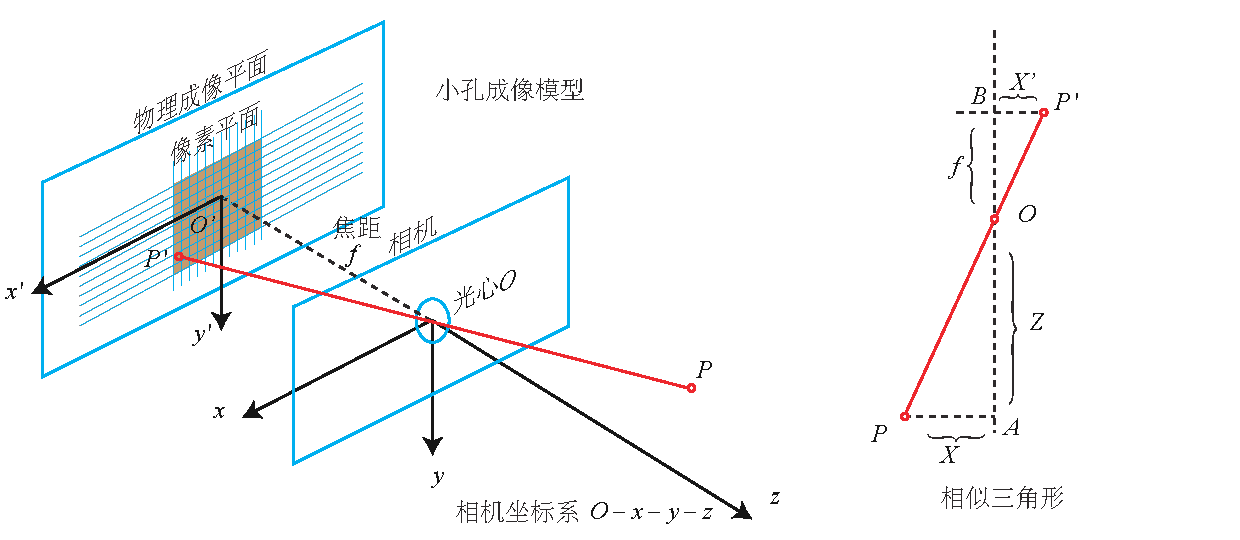
\includegraphics[width=.95\textwidth]{cameraModel/cameraModel.pdf}
	\caption{Pinhole camera model. }
	\label{fig:cameraModel}
\end{figure}

Let's take a look at the simple geometry in this model. Let $O-x-y-z$ be the camera coordinate system. Commonly we put the $z$ axis to the front of the camera, $x$ to the right, and $y$ to the down (so in this figure, we should stand on the left side to see the right side). $O$ is the camera's optical center, which is also the ``hole'' in the pinhole model. The 3D point $P$, after being projected through the hole $O$, falls on the physical imaging plane $O'-x'-y'$ and produces the image point $P'$. Let the coordinates of $P$ be $[X,Y,Z]^T$, $P'$ is $[X',Y',Z']^T$, and set the physical distance from the imaging plane to camera plane is $f$ (focal length). Then, according to the similarity of the triangles, there are:
\begin{equation}
\frac{Z}{f} = -\frac{X}{{X'}} =-\frac{Y}{{Y'}}.
\end{equation}

The negative sign indicates that the image is inverted. However, the image obtained by modern cameras is not inverted (otherwise, the usage of the camera would be very inconvenient). To make the model more realistic, we can equivalently place the imaging plane symmetrically in front of the camera, as shown by \autoref{fig:planes}. This can remove the negative sign in the formula to make it more compact:
\begin{equation}
\frac{Z}{f} = \frac{X}{{X'}} =\frac{Y}{{Y'}}.
\end{equation}

\begin{figure}[!htp]
	\centering
	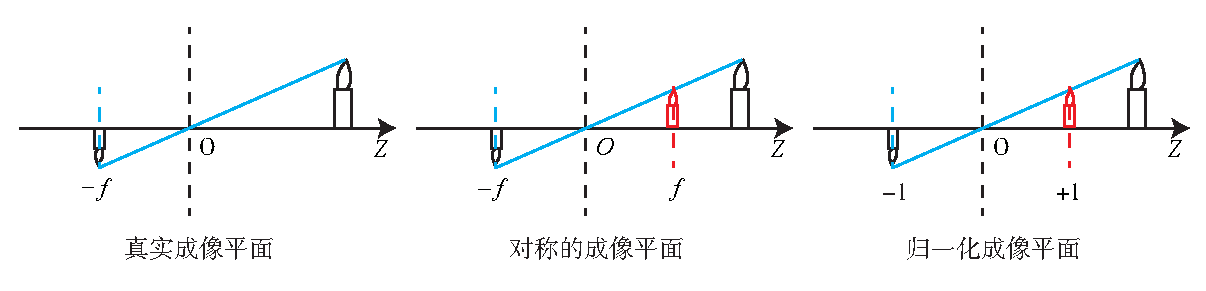
\includegraphics[width=1.0\textwidth]{cameraModel/planes.pdf}
	\caption{The real, symmetric and normalized image plane.}
	\label{fig:planes}
\end{figure}

Put $X', Y'$ to the left side:
\begin{equation}\label{eq:P2Pprime}
X' = f\frac{X}{Z}, \quad Y' = f\frac{Y}{Z}.
\end{equation}

Readers may ask why we can arbitrarily move the imaging plane to the front? In fact, this is just a mathematical approach to handle the camera projection, and most of the images captured by the camera are not upside-down. The camera's software will flip the picture for you, so what we actually get is the symmetric plane's image. Although the pin-hole image should be inverted from the physical principle since we have pre-processed the picture, it is not wrong to take the symmetric one. Therefore, without causing ambiguity, we often emit the minus symbol in the pin-hole model.


The formula~\eqref{eq:P2Pprime} describes the spatial relationship between the point $P$ and its image, where the units of all points are meters. For example, a focal length maybe 0.2 meters, and $X'$ be 0.14 meters. However, in the camera, we end up with pixels, where we need to sample and quantize the pixels on the imaging plane. To describe how the sensor converts the perceived light into image pixels, we set a pixel plane $o-u-v$ fixed on the physical imaging plane. Finally, we get \textit{pixel coordinates} of $P'$ in the pixel plane: $[u,v]^T$.

The usual definition of the pixel coordinate system \footnote{ Or image coordinate system, see section 2 of this lecture. } is: the origin $o'$ is in the upper left corner of the image, the $u$ axis is parallel to the $x$ axis, and the $v$ axis is parallel to the $y$ axis. Between the pixel coordinate system and the imaging plane, there is an apparent \textit{zoom} and a \textit{translation of the origin}. We set the pixel coordinates to scale $\alpha$ times on the $u$ axis and $\beta$ times on $v$. At the same time, the origin is translated by $[c_x, c_y]^T$. Then, the relationship between the coordinates of $P'$ and the pixel coordinate $[u,v]^T$ is:
\begin{equation}
\label{eq:project2pixel1} 
\left\{
\begin{matrix} 
u=\alpha X' + c_x\\ 
v=\beta Y' + c_y
\end{matrix}
\right. .
\end{equation}

Put it into~\eqref{eq:P2Pprime} and set $\alpha f$ as $f_x$, $\beta f$ as $f_y$:
\begin{equation}
\left\{
\begin{matrix} 
u=f_x\frac{X}{Z} + c_x\\ 
v=f_y\frac{Y}{Z} + c_y
\end{matrix}
\right. ,
\end{equation}
where $f$ is the focal length in meters, $\alpha, and \beta$ is in pixels/meter, so $f_x, f_y$ and $c_x, c_y$ are in pixels. It would be more compact to write this form as a matrix, but we need to use homogeneous coordinates on the left and non-homogeneous coordinates on the right:
\begin{equation}
\label{eq:intrinmatrix} 
\begin{pmatrix} u\\ v\\ 1 \end{pmatrix}=\frac{1}{Z}\begin{pmatrix} f_x & 0&c_x \\ 0& f_y& c_y\\ 0&0 & 1 \end{pmatrix}\begin{pmatrix} X\\ Y\\ Z \end{pmatrix} 
\buildrel \Delta \over =\frac{1}{Z} \mathbf{K} \mathbf{P}.
\end{equation}

Let's put $Z$ to the left side as in most books:
\begin{equation}
Z \begin{pmatrix} u\\ v\\ 1 \end{pmatrix}= \begin{pmatrix} f_x & 0&c_x \\ 0& f_y& c_y\\ 0&0 & 1 \end{pmatrix}\begin{pmatrix} X\\ Y\\ Z \end{pmatrix} 
\buildrel \Delta \over = \mathbf{K} \mathbf{P}.
\end{equation}

In this equation, we refer to the matrix composed of the middle quantities as the camera's inner parameter matrix (o intrinsics) $\mathbf{K}$. It is generally assumed that the camera's internal parameters are fixed after manufacturing and will not change during usage. Some camera manufacturers will tell you the intrinsics, and sometimes you need to estimate the internal parameters by yourself, which is called calibration. Because of the maturity of the calibration algorithm (such as the famous Zhang Zhengyou's calibration {\cite{Zhang1999}}), it will not be introduced here \footnote{I'm sure professor Zhang has a copy of this book now.}. 

There are internal parameters, and naturally, there must be something like ``external parameters''. In the equation ~\eqref{eq:intrinmatrix}~, we use the coordinates of $P$ in the camera coordinate system, but in fact, the coordinates of $P$ should be its world coordinates because the camera is moving (we use the symbol $\mathbf{P}_w$). It should be converted to the camera coordinate system based on the current pose of the camera. The camera's pose is described by its rotation matrix $\mathbf{R}$ and the translation vector $\mathbf{t}$. Then there are:

\begin{equation}
\label{eq:cameraprojection}
Z \mathbf{P}_{uv}=
Z \left[ \begin{array}{l}
u\\
v\\
1
\end{array} \right] = \mathbf{K} \left( {\mathbf{R}{ \mathbf{P}_w} + \mathbf{t}} \right) =  \mathbf{K} \mathbf{T} \mathbf{P}_w .
\end{equation}

Note that the latter formula implies a conversion from homogeneous to non-homogeneous coordinates (can you see it?) We use homogeneous coordinates in $\mathbf{T}\mathbf{P}$, then convert to non-homogeneous coordinates, and then multiply it by $\mathbf{K}$.  It describes the projection relationship of world coordinates to pixel coordinates of $P$. Among them, the camera's pose $\mathbf{R}, \mathbf{t}$ is also called the camera's \textit{extrinsics}. \footnote{In robots or autonomous vehicles, extrinsics is often defined as the transform between the camera coordinate system and the robot body coordinate system, describing ``where the camera is installed''.}  Compared with the intrinsic, the extrinsics may change with the camera installation and is also the target to be estimated in the SLAM if we only have a camera.

The projection process can also be viewed from another perspective. The formula ~\eqref{eq:cameraprojection} shows that we can convert a world coordinate point to the camera coordinate system first and then remove the last dimension. The depth of the point from the imaging plane of the camera is then removed, which is equivalent to the normalization on the last dimension. In this way, we get the projection of the point $P$ on the camera \textit{normalized plane}:
\begin{equation}
\left( {\mathbf{R}{\mathbf{P}_w} + \mathbf{t}} \right) = \underbrace{\left[ X,Y,Z\right]^T}_{\text{Camera Coordinates}} \to \underbrace {\left[ {X/Z,Y/Z,1} \right]^T}_{\text{Normalized Coordinates}}.
\end{equation}

The \textit{normalized coordinates} can be seen as a point in the $z=1$ plane in front of the camera \footnote{Note that in the calculation, it is necessary to check whether $Z$ is positive because the negative $Z$ can also get the point on the normalized plane by this method. However, the camera does not capture the scene behind the imaging plane. }.This $z=1$ plane is also called \textit{normalized plane}. We normalize the coordinates and then multiply them with the intrinsic matrix, yielding the pixel coordinates. We can also consider the pixel coordinates $[u,v]^T$ as the result of quantitative measurements on points on the normalized plane. If the camera coordinates are multiplied by any non-zero constant simultaneously, the normalized coordinates are the same, which means that the depth is lost during the projection process. So, in monocular vision, the pixel's depth value cannot be obtained by a single image.

\subsection{Distortion}
In order to get a larger FoV (Field-of-View), we usually add a lens in front of the camera. The addition of the lens has an influence on the propagation of light during imaging: (1) the shape of the lens may affect the propagation way of light, (2) during the mechanical assembly, the lens and the imaging plane are not entirely parallel, which also changes the projected position.

There are some mathematical models to describe the distortion caused by the shape of the lens. In the pinhole model, a straight line keeps straight when projected onto the pixel plane. However, in real photos, the camera lens tends to make a straight line in the real environment become a curve \footnote{Yes, it is no longer straight but becomes curved. If it makes an inside curve, it is called barrel-like distortion; otherwise, it is cushion-like distortion if the curve looks outward. }. The closer to the edge of the image, the more obvious this phenomenon is. Since the lenses actually produced are often center-symmetrical, this makes the irregular distortion generally radially symmetrical. They fall into two main categories: \textit{barrel-like distortion} and \textit{cushion-like distortion}, as shown by \autoref{fig:distortion}.
\begin{figure}[!t]
	\centering
	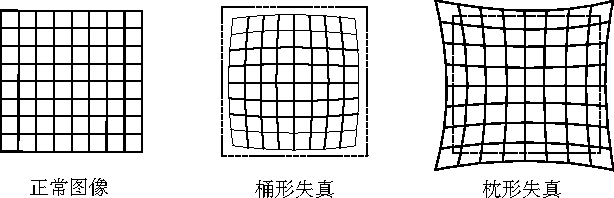
\includegraphics[width=0.7\textwidth]{cameraModel/distortion.pdf}
	\caption{The radical distortion.}
	\label{fig:distortion}
\end{figure}

In barrel distortion, the radius of pixels decreases as the optical axis's distance increases, while the cushion distortion is just the opposite. In both distortions, the line that intersects the center of the image and the optical axis remains the same.

In addition to the shape of the lens, which introduces radial distortion, \textit{tangential distortion} is introduced during assembly of the camera because the lens and the imaging surface cannot be strictly parallel, as shown by \autoref{fig:tangen}.

\begin{figure}[!t]
	\centering
	\includegraphics[width=0.7\textwidth]{cameraModel/tangen.pdf}
	\caption{Tangential distortion.}
	\label{fig:tangen}
\end{figure}
To better understand radial and tangential distortion, we describe them in a more rigorous mathematical form. Consider any point on the \textit{normalized plane}, $\mathbf{p}$, whose coordinates are $[x,y]^T$, or $[r, \theta]^T$ in the form of polar coordinates, where $r$ represents the distance between the point $\mathbf{p}$ and the origin of the coordinate system, and $\theta$ represents the angle to the horizontal axis. Radial distortion can be seen as a change in the coordinate point along the length, that is, its radius from the origin. Tangential distortion can be seen as a change in the coordinate point along the tangential direction, which means that the horizontal angle has changed. It is generally assumed that these distortions are polynomial, namely:
\begin{equation}
\label{eq:distortion} 
\begin{matrix}
x_\mathrm{distorted} = x(1+k_1r^2+k_2r^4+k_3r^6)\\
y_\mathrm{distorted} = y(1+k_1r^2+k_2r^4+k_3r^6)
\end{matrix},
\end{equation}
where $[x_\mathrm{distorted}, y_\mathrm{distorted}]^T$ is the \textit{normalized coordinates} of the point after distortion. On the other hand, for \textit{tangential distortion}, we can use the other two parameters $p_1,p_2$ to describe it:
\begin{equation}
\label{eq:tangen} 
\begin{matrix}
x_\mathrm{distorted} = x+2p_1xy+p_2(r^2+2x^2)\\
y_\mathrm{distorted} = y+p_1(r^2+2y^2)+2p_2xy
\end{matrix}. 
\end{equation}
Putting~\eqref{eq:distortion} and~\eqref{eq:tangen} together we get a joint model with 5 distortion coefficients. The complete form is:
\begin{equation}
\left\{\begin{matrix} x_\mathrm{distorted} =x(1+k_1r^2+k_2r^4+k_3r^6)+2p_1xy+p_2(r^2+2x^2)\\ 
y_\mathrm{distorted} = y(1+k_1r^2+k_2r^4+k_3r^6)+p_1(r^2+2y^2)+2p_2xy
\end{matrix}\right. .
\end{equation}

In the above process of correcting distortion, we used 5 distortion coefficients. In practical applications, you can flexibly choose to number of parameters, for example, only selecting $k_1, p_1, p_2$, or use $k_1, k_2, p_1, p_2$, etc.

This section models the camera's imaging process using a pinhole model and described the radial and tangential distortions caused by the lens. Researchers have proposed many other models in the existing imaging system, such as the affine model and perspective model, and there are many different types of distortion. In most visual SLAM systems, pinhole and rad-tan distortion models are sufficient, so we will not describe the other ones.

It is worth mentioning that there are two ways of undistortion (or correction). We can choose to undistort the entire image first, get the corrected image, and then discuss the spatial position of the points on the image. Alternatively, we can also extract some feature points in the distorted image and find its real position through the distortion equation. Both are feasible, but the former seems to be more common in visual SLAM. Therefore, when an image is undistorted, we can directly establish a projection relationship with the pinhole model without considering distortion. Therefore, in the discussion that follows, we can directly assume that the image has been undistorted.

Finally, let's summarize the imaging process of a monocular camera:

\begin{enumerate}
	\item First, there is a point $P$ in the world coordinate system, and its world coordinates are $\mathbf{P}_w$.
	\item Since the camera is moving, its motion is described by $\mathbf{R}, \mathbf{t}$ or  transform matrix $\mathbf{T} \in \mathrm{SE}(3)$. The camera coordinates for $P$ are $\tilde{\mathbf{P}}_c = \mathbf{R} \mathbf{P}_w + \mathbf{t}$.
	\item The $\tilde{\mathbf{P}}_c$ components are $X,Y, Z$, and they are projected onto the normalized plane $Z=1$ to get the normalized coordinates: $\mathbf{P}_c = [X/Z, Y/Z, 1]^T$. Note that $Z$ may be less than 1, indicating that the point is behind the normalization plane and it should not be projected on the camera plane.
	\item If the image is distorted, the coordinates of $\mathbf{P}_c$ after distortion are calculated according to the distortion parameters.
	\item Finally, the distorted coordinates of $P$ pass through the intrinsics and we find its pixel coordinates: $\mathbf{P}_{uv} = \mathbf{K} \mathbf{P}_c$.
\end{enumerate}

In summary, we have talked about four coordinates: the world coordinates, the camera coordinates, the normalized coordinates, and the pixel coordinates. Readers should clarify their relationship. They reflect the entire imaging process and will be used in the future.

\subsection{Stereo Cameras}
The pinhole camera model describes the imaging model of a single camera. However, we cannot determine the specific location of a spatial point only by a single pixel. This is because all points on the line from the camera's optical center to the normalized plane can be projected onto that pixel. Only when the depth of $P$ is determined (such as through a binocular or RGB-D camera) can we know exactly its spatial location, as shown in \autoref {fig:pixelLocation}~.

\begin{figure}[!ht]
    \centering
    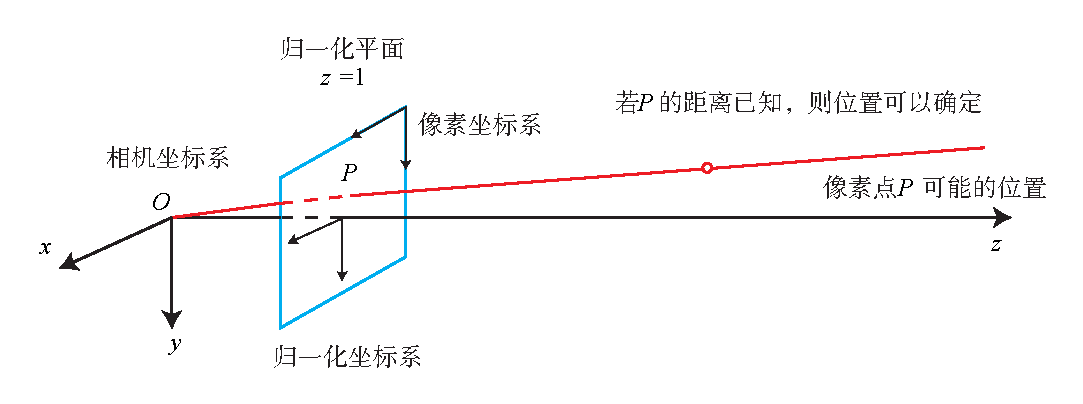
\includegraphics[width=1.0\textwidth]{cameraModel/pixelLocation.pdf}
    \caption{The possible location of a single pixel.}
    \label{fig:pixelLocation}
\end{figure}

There are many ways to measure the pixel distance (or depth). For example, the human eye can judge the object's distance according to the difference (or parallax) of the scene seen by the left and right eyes. The binocular camera principle is also the same. By simultaneously acquiring the left and right cameras' images and calculating the parallax/disparity between the images, each pixel's depth is estimated. In the following paragraph, we briefly describe the stereo camera's imaging principle (as shown in \autoref{fig:stereoCamera}~).

A binocular camera is generally composed of a left-eye camera and a right-eye camera. Of course, it can also be made up and down, but the mainstream binoculars we've seen are all left and right. Both the left and right cameras are regarded as simple pinhole cameras. They are synchronized and placed horizontally, meaning that both cameras' centers are on the same $x$ axis. The distance between the two centers is called \textit {baseline} (denoted as $b$), which is an important parameter.

\begin{figure}[!ht]
    \centering
    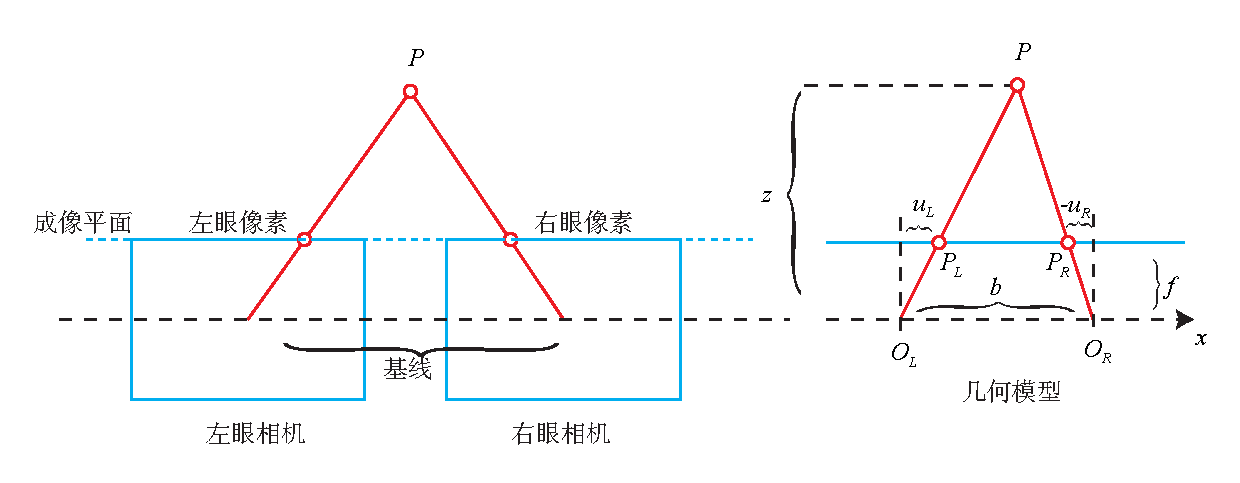
\includegraphics[width=1.0\textwidth]{cameraModel/stereoCamera.pdf}
    \caption{Geometry model of stereo cameras from upside down view. The $O_L, O_R$ are left and right optical centers. $f$ is the focal length, $u_L$ and $u_R$ are pixel coordinates of the same point along the $x$ axis. Note that $u_R$ should be a negative value in this figure, so the physical distance should be $-u_R$.}
    \label{fig:stereoCamera}
\end{figure}

Now consider a 3D point $P$, projected into the left-eye and the right-eye, written as $P_L, P_R$. Due to the presence of the camera baseline, these two imaging positions are different. Ideally, since the left and right cameras are only shifted on the $x$ axis, the image of $P$ also differs only on the $x$ axis (corresponding to the $u$ axis of the image). Take the left pixel coordinate as $u_L$ and the right coordinate as $u_R$. The geometric relationship is shown on the right of \autoref{fig:stereoCamera}. According to the similarity relationship between $ \triangle P P_L P_R$ and $\triangle P O_L O_R$, there are:

\begin{equation}
\frac{{z - f}}{z} = \frac{{b - {u_L} + {u_R}}}{b}.
\end{equation}

Rearrange it, and we have:
\begin{equation}
z = \frac{{fb}}{d}, \quad d \buildrel \Delta \over = {u_L} - {u_R},
\end{equation}
where $d$ is defined as the difference between the left and right figures' horizontal coordinates and is called disparity or parallax. Based on the parallax, we can estimate the distance between a pixel and the camera. Parallax is inversely proportional to distance: the larger the parallax is, the closer the distance is \footnote {Readers can simulate it with your own eyes.}. Simultaneously, since the parallax is at least one pixel, there is a theoretical maximum value for the binocular depth, which is determined by $fb$. To see the far-away things, we need a larger stereo camera; conversely, small binocular devices can only measure very close distances. By analogy, when the human eye looks at a very distant object (such as a very distant airplane), it is usually impossible to determine its distance accurately.

Although the depth's formula is simple, the real calculation of $d$ itself is more complicated. We need to know precisely where a pixel of the left-eye image appears in the right-eye image (that is, the corresponding relationship). This also belongs to the kind of task that is ``easy for humans but difficult for computers''. When we want to calculate each pixel's depth in an image, the calculation amount and accuracy will become a problem, and the parallax can be calculated only in the place where the image texture is rich. Due to the calculation amount, binocular depth estimation still needs GPU or FPGA to make the distance calculation run in real-time. This will be mentioned in lecture \ref{cpt:12}.

\subsection{RGB-D Cameras}
Compared to the binocular camera's way of calculating depth, the RGB-D camera's approach is more ``active'': it can actively measure each pixel's depth. The current RGB-D cameras can be divided into two categories according to their principle (see \autoref {fig:RGBDCamera} ~):

\begin{enumerate}
\item The first kind of RGB-D sensor uses structured infrared light to measure pixel distance. Many of the old RGB-D sensors are belong to this kind, for example, the Kinect 1st generation, Project Tango 1st generation, Intel RealSense, etc.
\item The second kind measures pixel distance using the \textit{time-of-flight (ToF)}. Examples are Kinect 2 and some existing ToF sensors in cellphones.
\end{enumerate}

\begin{figure}[!ht]
    \centering
    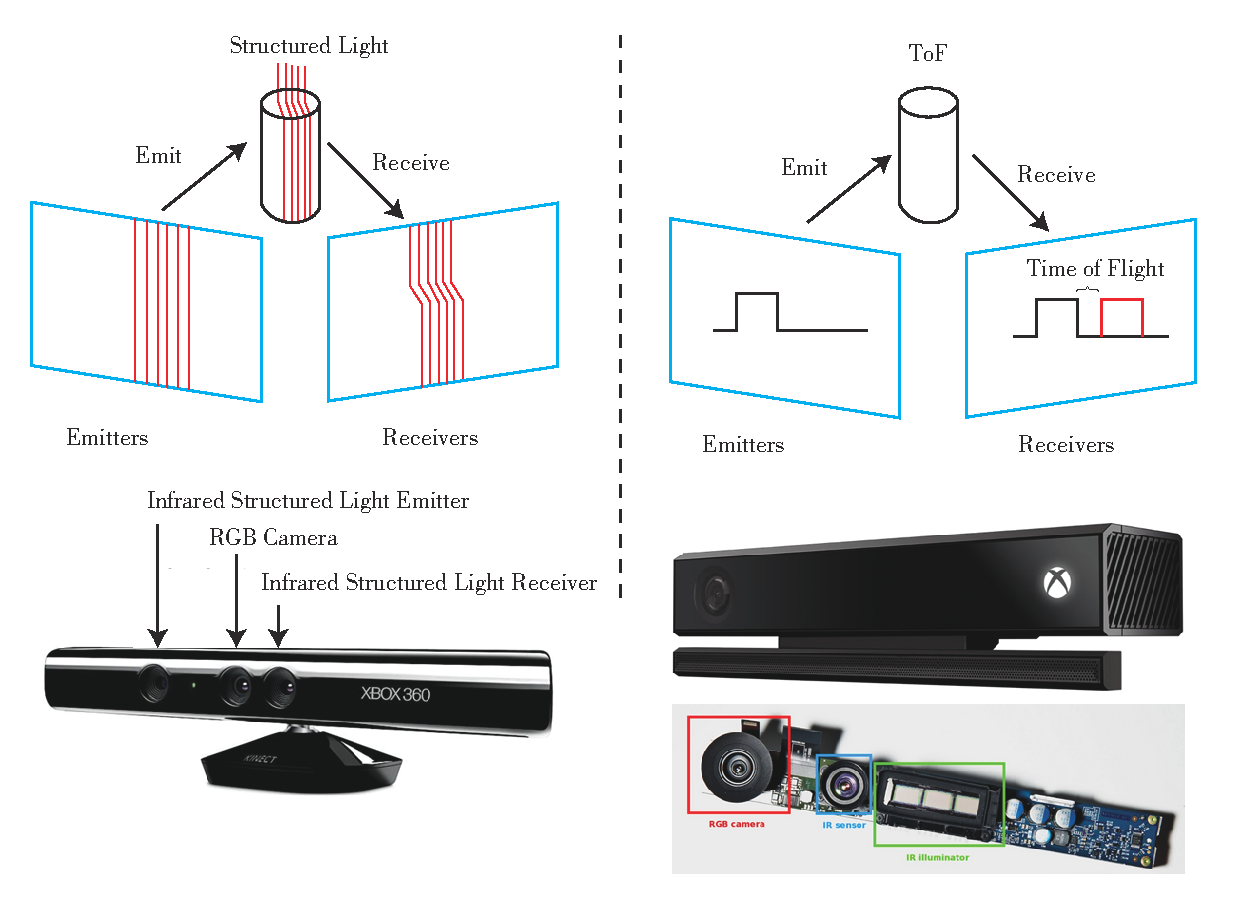
\includegraphics[width=1.0\textwidth]{cameraModel/rgbdCamera.pdf}
    \caption{RGB-D Cameras}
    \label{fig:RGBDCamera}
\end{figure}

Regardless of the type, the RGB-D camera needs to emit a light beam (usually infrared light) to the target object. In the structured light principle, the camera calculates the distance between the object and itself based on the returned structured light pattern. In the ToF principle, the camera emits a light pulse to the target and then determines the distance according to the beam's time of flight. The ToF principle is very similar to the laser sensor, except that the laser obtains the distance by scanning point by point (or line by line). The ToF camera can obtain the entire image's pixel depth, which is also the RGB-D camera's main advantage. So, if you take apart an RGB-D camera, you will usually find that there will be at least one transmitter and one receiver in addition to the ordinary camera.

After measuring the depth, the RGB-D camera usually completes the pairing between the depth and color map pixels according to each camera's position at the time of production. It outputs a pixel-to-pixel corresponding color image and depth image. We can read the color information and distance information at the same image position, calculate the 3D camera coordinates of the pixels, and generate a point cloud. RGB-D data can be processed either at the image level or the point cloud level. The second experiment of this lecture will demonstrate the point cloud construction of RGB-D cameras.

The RGB-D camera can measure the distance of each pixel in real-time. However, due to this measurement of transmitting and receiving, its range of use is limited. RGB-D cameras that use infrared light for depth measurement are susceptible to interference from infrared light emitted by daylight or other sensors, so they cannot be used outdoors. Without modulation, multiple RGB-D cameras can interfere with each other. These points' positions cannot be measured for transparent objects because they cannot receive reflected light. Also, RGB-D cameras have some disadvantages in terms of cost and power consumption.

\section{Images}
Cameras and lens convert the information in the three-dimensional world into a photo composed of pixels, which is then stored in the computer as a data source for subsequent processing. In mathematics, images can be described by a matrix; in computers, they occupy a continuous disk or memory space, which can be represented by a two-dimensional array. In this way, the program does not have to distinguish whether they are dealing with a numerical matrix or a meaningful image.

In this section, we will introduce some basic operations of computer image processing. In particular, we are going to introduce the basic steps of processing images with OpenCV and lay the foundation for subsequent chapters. Let's start with the simplest case, the grayscale image. Each pixel position $ (x, y) $ corresponds to a grayscale value of $ I $ in a grayscale image. Therefore, an image with the width of $ w $ and the height of $ h $ can be mathematically written as a function:
\[
(I) (x, y): \mathbb {R} ^ 2 \mapsto \mathbb {R},
\]
where $ (x, y) $ is the coordinate of the pixel. However, computers cannot express real numbers, so we need to quantify the subscripts and image readings within a certain range. For example, $ x, y $ are usually integers starting with 0 to $w-1, h-1$. In common grayscale images, an integer of $0 \textasciitilde 255$ (that is, an unsigned char in C++, 1 byte) is used to express the grayscale reading of the image. Then, a grayscale image with a width of 640 pixels and a height of 480 pixels can be expressed as:
\begin{lstlisting}[language=C++, caption=Use 2D array to express an image]
unsigned char image[480][640];
\end{lstlisting}

Why does the two-dimensional array here have the size of 480 $ \times $ 640? Because in the program, the first index of the 2D array is the row, and the second index is the column. In an image, the number of rows (or the $y$ axis) in the array corresponds to the height of the image, and the number of columns (or the $x$ axis) corresponds to the width of the image.
\begin{figure}[!t]
    \centering
    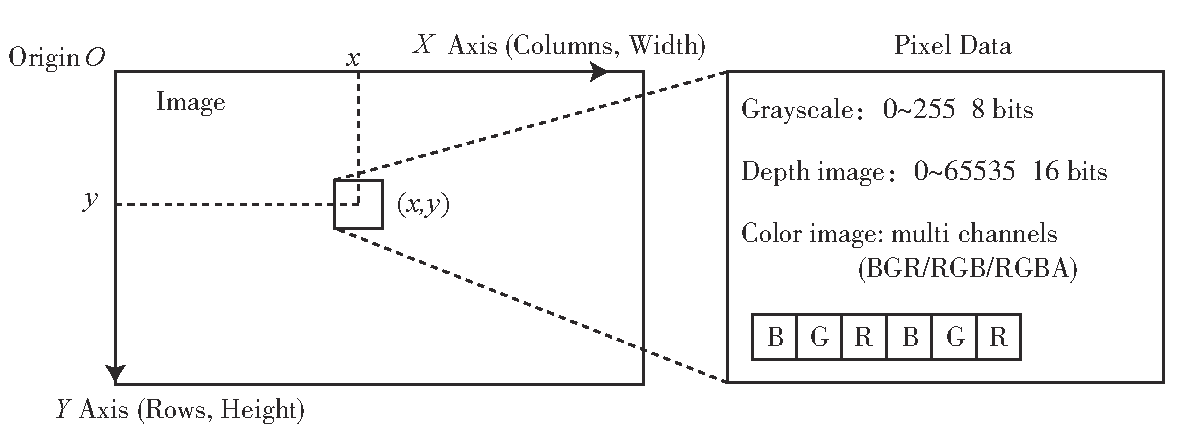
\includegraphics[width=0.84\textwidth]{cameraModel/image.pdf}
    \caption{Pixels in an image.}
    \label{fig:imagesInComputer}
\end{figure}

Let's examine the content of this image. Images are naturally made up of pixels. When accessing a certain pixel, you need to specify its coordinates, as shown in \autoref{fig:imagesInComputer}~. The left side of the figure shows how the traditional pixel coordinate system is defined. The origin is in the upper left corner of the image, the $X$ axis is from left to right, and the $Y$ is top-down. If it has a third axis, the $ Z $ axis, then according to the right-hand rule, the $ Z $ axis should be from outside to inside (or front in 3D space). This definition is consistent with the camera coordinate system. The width or number of columns of an image corresponds to the $ X $ axis; the number of rows or the height of an image corresponds to its $ Y $ axis.

According to this definition, if we discuss a pixel located at $x,y$, then the code of accessing its memory in the computer should be:
\begin{lstlisting}[language = C++, caption = Accessing image pixels]
unsigned char pixel = image[y][x];
\end{lstlisting}

It corresponds to the reading of the gray value $ I(x,y) $. Please note the order of $ x $ and $ y $ here. Although we tirelessly discuss the problem of coordinate systems, errors like this index sequence will still be one of the most common errors encountered by novices during debugging. If you accidentally change the coordinates of $ x, y $ when writing a program, the compiler cannot provide any useful information at compile-time. All you can see is a segment fault in runtime.

A pixel's grayscale can be recorded as an 8-bit unsigned integer, which is a value of $0\textasciitilde 255$. If we have more information to record, one byte is probably not enough. For example, in the depth map of an RGB-D camera, each pixel's distance is recorded. This distance is usually measured in millimeters, and the range of RGB-D cameras is usually around a dozen meters, exceeding 255. At this time, people will use 16-bit integers (unsigned short in C++) to record the depth map information, that is, the value at $0 \textasciitilde 65535$. When converted to meters, it can represent up to 65 meters, which is enough for RGB-D cameras.

The representation of a color image requires the concept of a channel. In computers, we use three colors: red, green, and blue to express any color. Therefore, for each pixel, three R, G, and B values are recorded, and each value is called a channel. For example, the most common color image has three channels, represented by an 8-bit integer. Under this rule, one pixel occupies a 24-bit space.

The number and order of channels can be freely defined. In OpenCV color images, the default order of channels is B, G, R, which means when we get a 24-bit pixel, the first 8 bits represent the blue value, the middle 8 bits represent the green, and the last 8 bits represent the red. Similarly, the order of R, G, and B can also be used to describe a color image. If you want to express the image's transparency, use R, G, B, A four channels.

\section{Practice: Images in Computer Vision}
\subsection{Basic Usage of OpenCV}
The following is a demo program to help you understand how to access the image in OpenCV and how to visit its pixels.

\subsubsection{Install OpenCV}
OpenCV \footnote {Official homepage: \url{http://opencv.org}. } provides many open-source image algorithms and is a very widely used image processing algorithm library in computer vision. This book also uses OpenCV for basic image processing. Before using, readers must install it from the pre-compiled library or from source code. Under Ubuntu, there are two options: \textit{install from source code} or \textit {only install binary library files}:

\begin{enumerate}
\item Install from source means to download all OpenCV source code from the OpenCV website, compile and install on the machine for usage. The advantage is that you can freely choose which version to install, and the source code is accessible, but it takes some compilation time.
\item Or, we can only install the binary library file, which means it was pre-compiled by the Ubuntu community, so there is no need to recompile it.
\end{enumerate}

If we use a newer version of OpenCV than that in the apt source, we must install it from the source code. First, you can adjust some compilation options to match the programming environment (for example, to disable some unused modules or turn on the GPU acceleration, etc.). OpenCV currently maintains two major versions, divided into OpenCV 2.4 series and OpenCV 3 series \footnote{In 2020, we can also use version 4.0 or higher.}. This book uses the OpenCV \textit {3} or higher.

Because the OpenCV project is relatively large, it will not be placed under 3rdparty in this book. Readers can download it from ~ \url{http://opencv.org/downloads.html}~ and select the Linux version. You will get a compressed package like opencv-3.1.0.zip. Unzip it to any directory, we can found that OpenCV is also a CMake project.

Before compiling, first, install the dependencies of OpenCV:
\begin{lstlisting}[language=sh, caption=Terminal input:]
sudo apt-get install build-essential libgtk2.0-dev libvtk5-dev libjpeg-dev libtiff4-dev libjasper-dev libopenexr-dev libtbb-dev
\end{lstlisting}

In fact, OpenCV has many dependencies, and the lack of certain dependency items will affect some of its functions (but we will not use all the functions). OpenCV will check whether the dependencies will be installed during CMake and adjust its own configurations. If you have a GPU on your computer and the relevant dependencies are installed, OpenCV will also enable GPU acceleration. But for this book, the above dependencies are sufficient.

Subsequent compilation and installation are the same as ordinary CMake projects. After make, please call ``sudo make install'' to install OpenCV on your machine (instead of just compiling it). Depending on the machine configuration, this compilation process may take from 20 minutes to an hour. If your CPU is powerful, you can use commands like ``make -j4'' to call multiple threads to compile (the parameter after -j is the number of threads used). After installation, OpenCV is stored in the /usr/local directory by default. You can look for OpenCV header files and library files' installation location to see where they are. Besides, if you have installed the OpenCV 2 series before, it is recommended that you install OpenCV 3 elsewhere (think about how this should be done).

\subsection{Basic OpenCV Images Operations}
Now let's go through the basic image operations in OpenCV from a simple example.

\begin{lstlisting}[language=C++,caption=slambook/ch5/imageBasics/imageBasics.cpp]
#include <iostream>
#include <chrono>

using namespace std;

#include <opencv2/core/core.hpp>
#include <opencv2/highgui/highgui.hpp>

int main(int argc, char **argv) {
    // Read the image in argv[1]
    cv::Mat image;
    image = cv::imread(argv[1]); // call cv::imread to read the image from file
    
    // check the data is correctly loaded
    if (image.data == nullptr) { // maybe the file does not exist
        cerr << "file" << argv[1] << " not exist." << endl;
        return 0;
    }
    
    // print some basic information
    cout << "Image cols: " << image.cols << ", rows: " << image.rows 
	    << ", channels: " << image.channels() << endl;
    cv::imshow("image", image);      // use cv::imshow to show the image
    cv::waitKey(0);                  // display and wait for a keyboard input
    
    // check image type
    if (image.type() != CV_8UC1 && image.type() != CV_8UC3) {
        // we need grayscale image or RGB image
        cout << "image type incorrect." << endl;
        return 0;
    }
    
    // check hte pixels
    chrono::steady_clock::time_point t1 = chrono::steady_clock::now();
    for (size_t y = 0; y < image.rows; y++) {
        // use cv::Mat::ptr to get the pointer of each row
        unsigned char *row_ptr = image.ptr<unsigned char>(y);  // row_ptr is the pointer to y-th row
        for (size_t x = 0; x < image.cols; x++) {
            // read the pixel on (x,y), x=column, y=row
            unsigned char *data_ptr = &row_ptr[x * image.channels()]; // data_ptr is the pointer to (x,y)
            // visit the pixel in each channel
            for (int c = 0; c != image.channels(); c++) {
                unsigned char data = data_ptr[c]; // data should be pixel of I(x,y) in c-th channel
            }
        }
    }
    chrono::steady_clock::time_point t2 = chrono::steady_clock::now();
    chrono::duration<double> time_used = chrono::duration_cast < chrono::duration < double >> (t2 - t1);
    cout << "time used: " << time_used.count() << " seconds." << endl;
    
    // copying cv::Mat
    // operator = will not copy the image data, but only the reference
    cv::Mat image_another = image;
    // changing image_another will also change image 
    image_another(cv::Rect(0, 0, 100, 100)).setTo(0); // set top-left 100*100 block to zero
    cv::imshow("image", image);
    cv::waitKey(0);
    
    // use cv::Mat::clone to actually clone the data
    cv::Mat image_clone = image.clone();
    image_clone(cv::Rect(0, 0, 100, 100)).setTo(255);
    cv::imshow("image", image);
    cv::imshow("image_clone", image_clone);
    cv::waitKey(0);
    
    // We are not going to copy the OpenCV's documentation here
    // please take a look at it for other image operations like clipping, rotating and scaling.
    
    cv::destroyAllWindows();
    return 0;
}
\end{lstlisting}

In this example, we demonstrated the following operations: image reading, displaying, pixel vising, copying, assignment, etc. When compiling the program, you need to add the OpenCV header file in your ``CMakeLists.txt'', and then link the program to the OpenCV's library. At the same time, due to the use of C++ 11 standards (such as the nullptr and chrono), you also need to set up the c++ standard in the compiler flag:

\begin{lstlisting}[language=Python,caption=slambook/ch5/imageBasics/CMakeLists.txt]
# use c++11 standard
set( CMAKE_CXX_FLAGS "-std=c++11" )

# find OpenCV
find_package( OpenCV REQUIRED )
# include its headers
include_directories( ${OpenCV_INCLUDE_DIRS} )

add_executable( imageBasics imageBasics.cpp )

# link the exe to opencv's libs
target_link_libraries( imageBasics ${OpenCV_LIBS} )
\end{lstlisting}

Let's give some notes for the code:
\begin{enumerate}
\item The program reads the image position from argv[1], the first parameter on the command line. We prepared an image (ubuntu.png, an Ubuntu wallpaper, hope you like it) for readers to test. Therefore, after compilation, use the following command to call this program:
\begin{lstlisting}[language=sh, caption=Terminal input:]
./build/imageBasics ubuntu.png
\end{lstlisting}
If you call this program in the IDE, be sure to give it parameters at the same time. This can be configured in the launch configuration dialog if you are using Clion.
\item In line 10 \textasciitilde to 18, we use the cv::imread function to read the image. And then, we display the image and its basic information.
\item In line 35 \textasciitilde 46, we iterate over all pixels in the image and calculates the time spent in the entire loop. Please note that the pixel visiting method is not unique, and the method given by the example is not the most efficient way. OpenCV provides an iterator of cv::Mat. You can traverse the pixels of the image through the iterator. Or, cv::Mat::data provides a raw pointer to the beginning of the image data. You can also directly calculate the offset through this pointer, and then get the memory location of the pixel. The method used in the example is to facilitate the reader to understand the structure of the image.

\item OpenCV provides many functions for manipulating images. We will not list them one by one. Otherwise, this book will become an OpenCV operation manual. The example shows the most common things like image reading and displaying and the deep copy function in cv::Mat. During the programming process, readers will also encounter operations such as image rotation and interpolation. At this time, you should refer to the corresponding documentation of the function to understand their principles and usage.
\end{enumerate}

It should be noted that OpenCV is not the only image library. It is just one of the more widely used ones. However, most image libraries have similar image operations. We hope that readers can understand the representation of images in other libraries after using OpenCV to quickly adjust to any other libraries. Since cv::Mat is also a matrix class, we can also use it to store matrix data such as rotation matrix and do some linear algebra operations. But it is generally believed that \textit{Eigen} is more efficient for use with fixed-size matrices.

\subsection{Image Undistortion}
We've introduced the rad-tan distortion model in the previous section, now let write an example to show the implementation. OpenCV has provided the cv::Undistort function for us, but we will also give a hand-written undistortion function to show the principles.

\begin{lstlisting}[language=C++,caption=slambook/ch5/imageBasics/undistortImage.cpp]
#include <opencv2/opencv.hpp>
#include <string>
using namespace std;
string image_file = "./distorted.png";   // the distorted image 

int main(int argc, char **argv) {
    // In thie program we implement the undistortion by ourselves rather than using opencv
    // rad-tan model params
    double k1 = -0.28340811, k2 = 0.07395907, p1 = 0.00019359, p2 = 1.76187114e-05;
    // intrinsics
    double fx = 458.654, fy = 457.296, cx = 367.215, cy = 248.375;
    
    cv::Mat image = cv::imread(image_file, 0);   // the image type is CV_8UC1
    int rows = image.rows, cols = image.cols;
    cv::Mat image_undistort = cv::Mat(rows, cols, CV_8UC1);   // the undistorted image
    
    // computate the pixels in the undistorted one
    for (int v = 0; v < rows; v++) {
        for (int u = 0; u < cols; u++) {
            // note we are computing the pixel of (u,v) in the undistorted image
            // according to the rad-tan model, compute the coordinates in the distorted image
            double x = (u - cx) / fx, y = (v - cy) / fy;
            double r = sqrt(x * x + y * y);
            double x_distorted = x * (1 + k1 * r * r + k2 * r * r * r * r) + 2 * p1 * x * y + p2 * (r * r + 2 * x * x);
            double y_distorted = y * (1 + k1 * r * r + k2 * r * r * r * r) + p1 * (r * r + 2 * y * y) + 2 * p2 * x * y;
            double u_distorted = fx * x_distorted + cx;
            double v_distorted = fy * y_distorted + cy;
            
            // check if the pixel is in the image boarder
            if (u_distorted >= 0 && v_distorted >= 0 && u_distorted < cols && v_distorted < rows) {
                image_undistort.at<uchar>(v, u) = image.at<uchar>((int) v_distorted, (int) u_distorted);
            } else {
                image_undistort.at<uchar>(v, u) = 0;
            }
        }
    }
    
    // show the undistorted image
    cv::imshow("distorted", image);
    cv::imshow("undistorted", image_undistort);
    cv::waitKey();
    return 0;
}
\end{lstlisting}

Please check the difference between the two images by yourself.

\section{Practice: 3D Vision}
\subsection{Stereo Vision}
We have introduced the imaging principle of stereo vision. Now we start from the left and right images, calculate the disparity map corresponding to the left eye, and then calculate each pixel's coordinates in the camera coordinate system, which will form a \textit{point cloud}. We have prepared left and right images for the readers, as shown in \autoref {fig:stereoExample}. The following code demonstrates the calculation of disparity map and point cloud:

\begin{lstlisting}[language=C++,caption=slambook/ch5/stereoVision/stereoVision.cpp (Part)]
int main(int argc, char **argv) {
    // intrinsics
    double fx = 718.856, fy = 718.856, cx = 607.1928, cy = 185.2157;
    // baseline
    double b = 0.573;
    
    cv::Mat left = cv::imread(left_file, 0);
    cv::Mat right = cv::imread(right_file, 0);
    cv::Ptr<cv::StereoSGBM> sgbm = cv::StereoSGBM::create(
        0, 96, 9, 8 * 9 * 9, 32 * 9 * 9, 1, 63, 10, 100, 32);    // SGBM is senstive to parameters
    cv::Mat disparity_sgbm, disparity;
    sgbm->compute(left, right, disparity_sgbm);
    disparity_sgbm.convertTo(disparity, CV_32F, 1.0 / 16.0f);
    
    // compute the point cloud
    vector<Vector4d, Eigen::aligned_allocator<Vector4d>> pointcloud;
    
    // change v++ and u++ to v+=2, u+=2 if your machine is slow to get a sparser cloud
    for (int v = 0; v < left.rows; v++)
    for (int u = 0; u < left.cols; u++) {
        if (disparity.at<float>(v, u) <= 10.0 || disparity.at<float>(v, u) >= 96.0) continue;
        
        Vector4d point(0, 0, 0, left.at<uchar>(v, u) / 255.0); // the first three dimensions are xyz, the 4-th is the color
        
        // compute the depth from disparity
        double x = (u - cx) / fx;
        double y = (v - cy) / fy;
        double depth = fx * b / (disparity.at<float>(v, u));
        point[0] = x * depth;
        point[1] = y * depth;
        point[2] = depth;
        
        pointcloud.push_back(point);
    }
    
    cv::imshow("disparity", disparity / 96.0);
    cv::waitKey(0);
    
    // show the point cloud in pangolin
    showPointCloud(pointcloud);
    return 0;
}
\end{lstlisting}

\begin{figure}[!t]
    \centering
    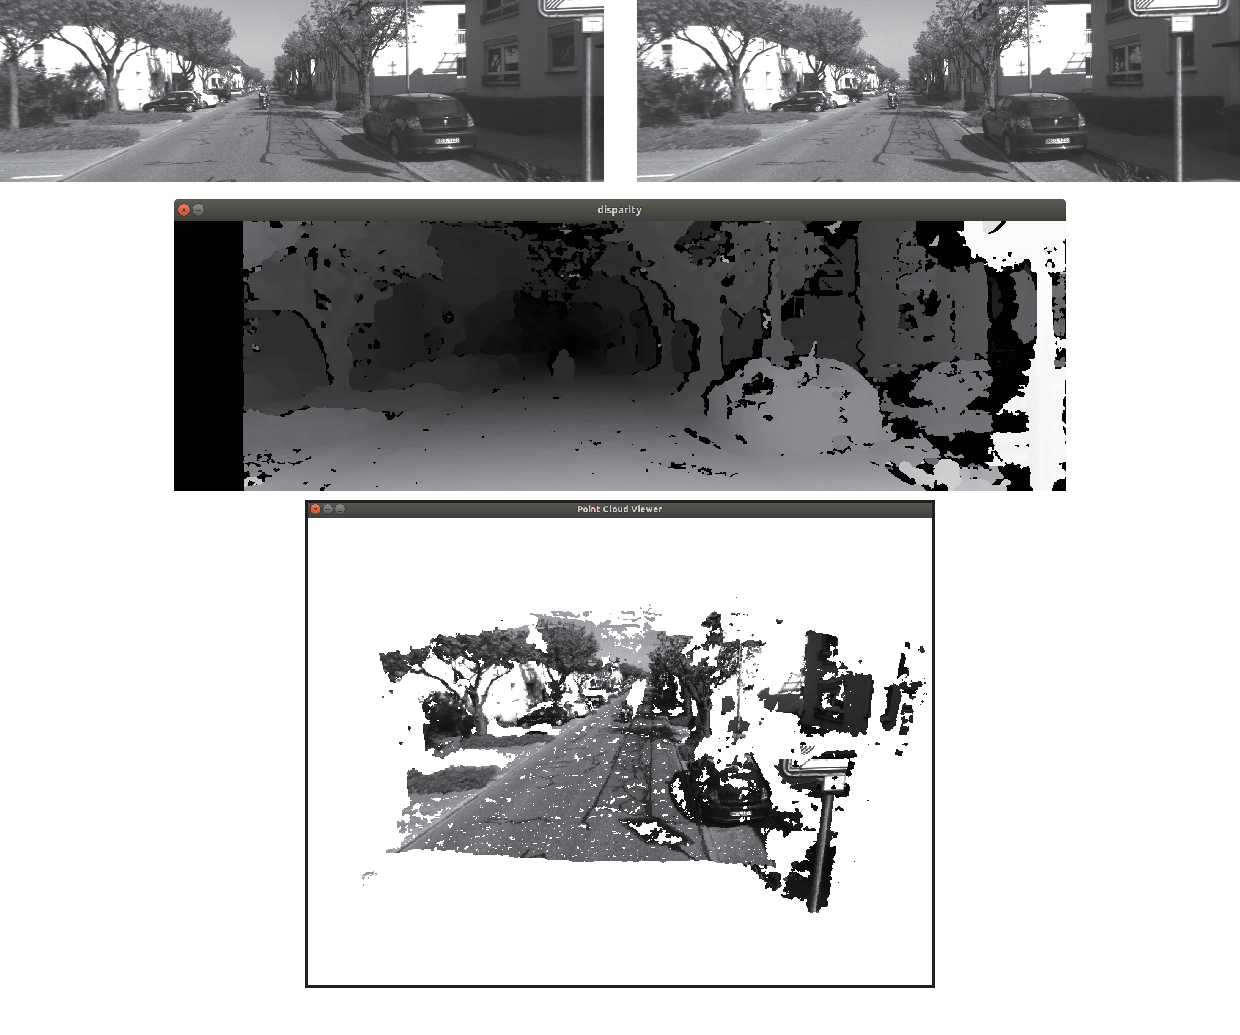
\includegraphics[width=0.9\textwidth]{cameraModel/stereoExample.pdf}
    \caption{Stereo image example. Top-left: left image, top-right: right image, mid: SGBM disparity map, bottom: point cloud. Note that since some of the pixels in the left image is not seen in the right one, so the disparity map will have some empty values.}
    \label{fig:stereoExample}
\end{figure}

In this example, we call the SGBM (Semi-global Batch Matching) {\cite{Hirschmuller2008}} algorithm implemented by OpenCV to calculate the disparity of the left and right images and then transform it into the 3D space of the camera through the geometric model of the binocular camera. We use a classic parameter configuration from the internet, and we mainly adjust the maximum and minimum disparity. The disparity data combined with the camera's internal parameters and baseline can determine each point's position in three-dimensional space. We omit the code related to displaying the point cloud to save some space.

This book is not going to introduce the disparity calculation algorithm of the binocular camera. Interested readers can read the relevant references {\cite{Scharstein2002, Seitz2006}}. In addition to the binocular algorithm implemented by OpenCV, there are many other libraries focused on achieving efficient parallax calculations. It is still an active and complex subject today.

\subsection{RGB-D Vision}
\label{sec:join-point-cloud}
Finally, we demonstrate an example of RGB-D vision. The convenience of RGB-D cameras is that they can obtain pixel depth information through physical methods. If the camera's intrinsic and extrinsic are known, we can calculate any pixel position in the world coordinate system, thereby creating a point cloud map. Now let's demonstrate how to do it.

We have prepared 5 pairs of images located in the slambook2/ch5/rgbd folder. There are 5 RGB images from 1.png to 5.png under the color/ directory and 5 corresponding depth images under the depth/. At the same time, the ``pose.txt'' file gives the camera poses of the 5 images (in the form of $ \mathbf{T}_\mathrm{wc} $). The format of the pose record is the same as before, with the translation vector plus a rotation quaternion:
\[
[x, y, z, q_x, q_y, q_z, q_w],
\]
where $q_w$ is the real part of the quaternion. For example, the parameters of the first pair of image are:
\[
[-0.228993, 0.00645704, 0.0287837, -0.0004327, -0.113131, -0.0326832, 0.993042].
\]

Below we write a program to accomplish two things: (1) We calculate the point cloud corresponding to each pair of RGB-D images based on internal parameters; (2) According to the camera pose of each image, we put the points to a global cloud by the camera poses.

\begin{lstlisting}[language=C++,caption=slambook/ch5/rgbd/jointMap.cpp (Part)]
int main(int argc, char **argv) {
    vector<cv::Mat> colorImgs, depthImgs;
    TrajectoryType poses;         // camera poses
    
    ifstream fin("./pose.txt");
    if (!fin) {
        cerr << "Please run the program in the directory that has pose.txt" << endl;
        return 1;
    }
    
    for (int i = 0; i < 5; i++) {
        boost::format fmt("./%s/%d.%s"); // the image format
        colorImgs.push_back(cv::imread((fmt % "color" % (i + 1) % "png").str()));
        depthImgs.push_back(cv::imread((fmt % "depth" % (i + 1) % "pgm").str(), -1)); // use -1 flag to load the depth image
        
        double data[7] = {0};
        for (auto &d:data) fin >> d;
        Sophus::SE3d pose(Eigen::Quaterniond(data[6], data[3], data[4], data[5]),
        Eigen::Vector3d(data[0], data[1], data[2]));
        poses.push_back(pose);
    }
    
    // compute the point cloud using camera intrinsics
    double cx = 325.5;
    double cy = 253.5;
    double fx = 518.0;
    double fy = 519.0;
    double depthScale = 1000.0;
    vector<Vector6d, Eigen::aligned_allocator<Vector6d>> pointcloud;
    pointcloud.reserve(1000000);
    
    for (int i = 0; i < 5; i++) {
        cout << "Converting RGBD images " << i + 1 << endl;
        cv::Mat color = colorImgs[i];
        cv::Mat depth = depthImgs[i];
        Sophus::SE3d T = poses[i];
        for (int v = 0; v < color.rows; v++)
        for (int u = 0; u < color.cols; u++) {
            unsigned int d = depth.ptr<unsigned short>(v)[u]; // depth value is 16-bit
            if (d == 0) continue; // 0 means no valid value
            Eigen::Vector3d point;
            point[2] = double(d) / depthScale;
            point[0] = (u - cx) * point[2] / fx;
            point[1] = (v - cy) * point[2] / fy;
            Eigen::Vector3d pointWorld = T * point;
            
            Vector6d p;
            p.head<3>() = pointWorld;
            p[5] = color.data[v * color.step + u * color.channels()];   // blue
            p[4] = color.data[v * color.step + u * color.channels() + 1]; // green
            p[3] = color.data[v * color.step + u * color.channels() + 2]; // red
            pointcloud.push_back(p);
        }
    }
    
    cout << "global point cloud has " << pointcloud.size() << " points." << endl;
    showPointCloud(pointcloud);
    return 0;
}
\end{lstlisting}

We can see the point cloud in \textit{Pangolin} after building it (see \autoref{fig:pointcloudmapping}).

\begin{figure}[!t]
    \centering
    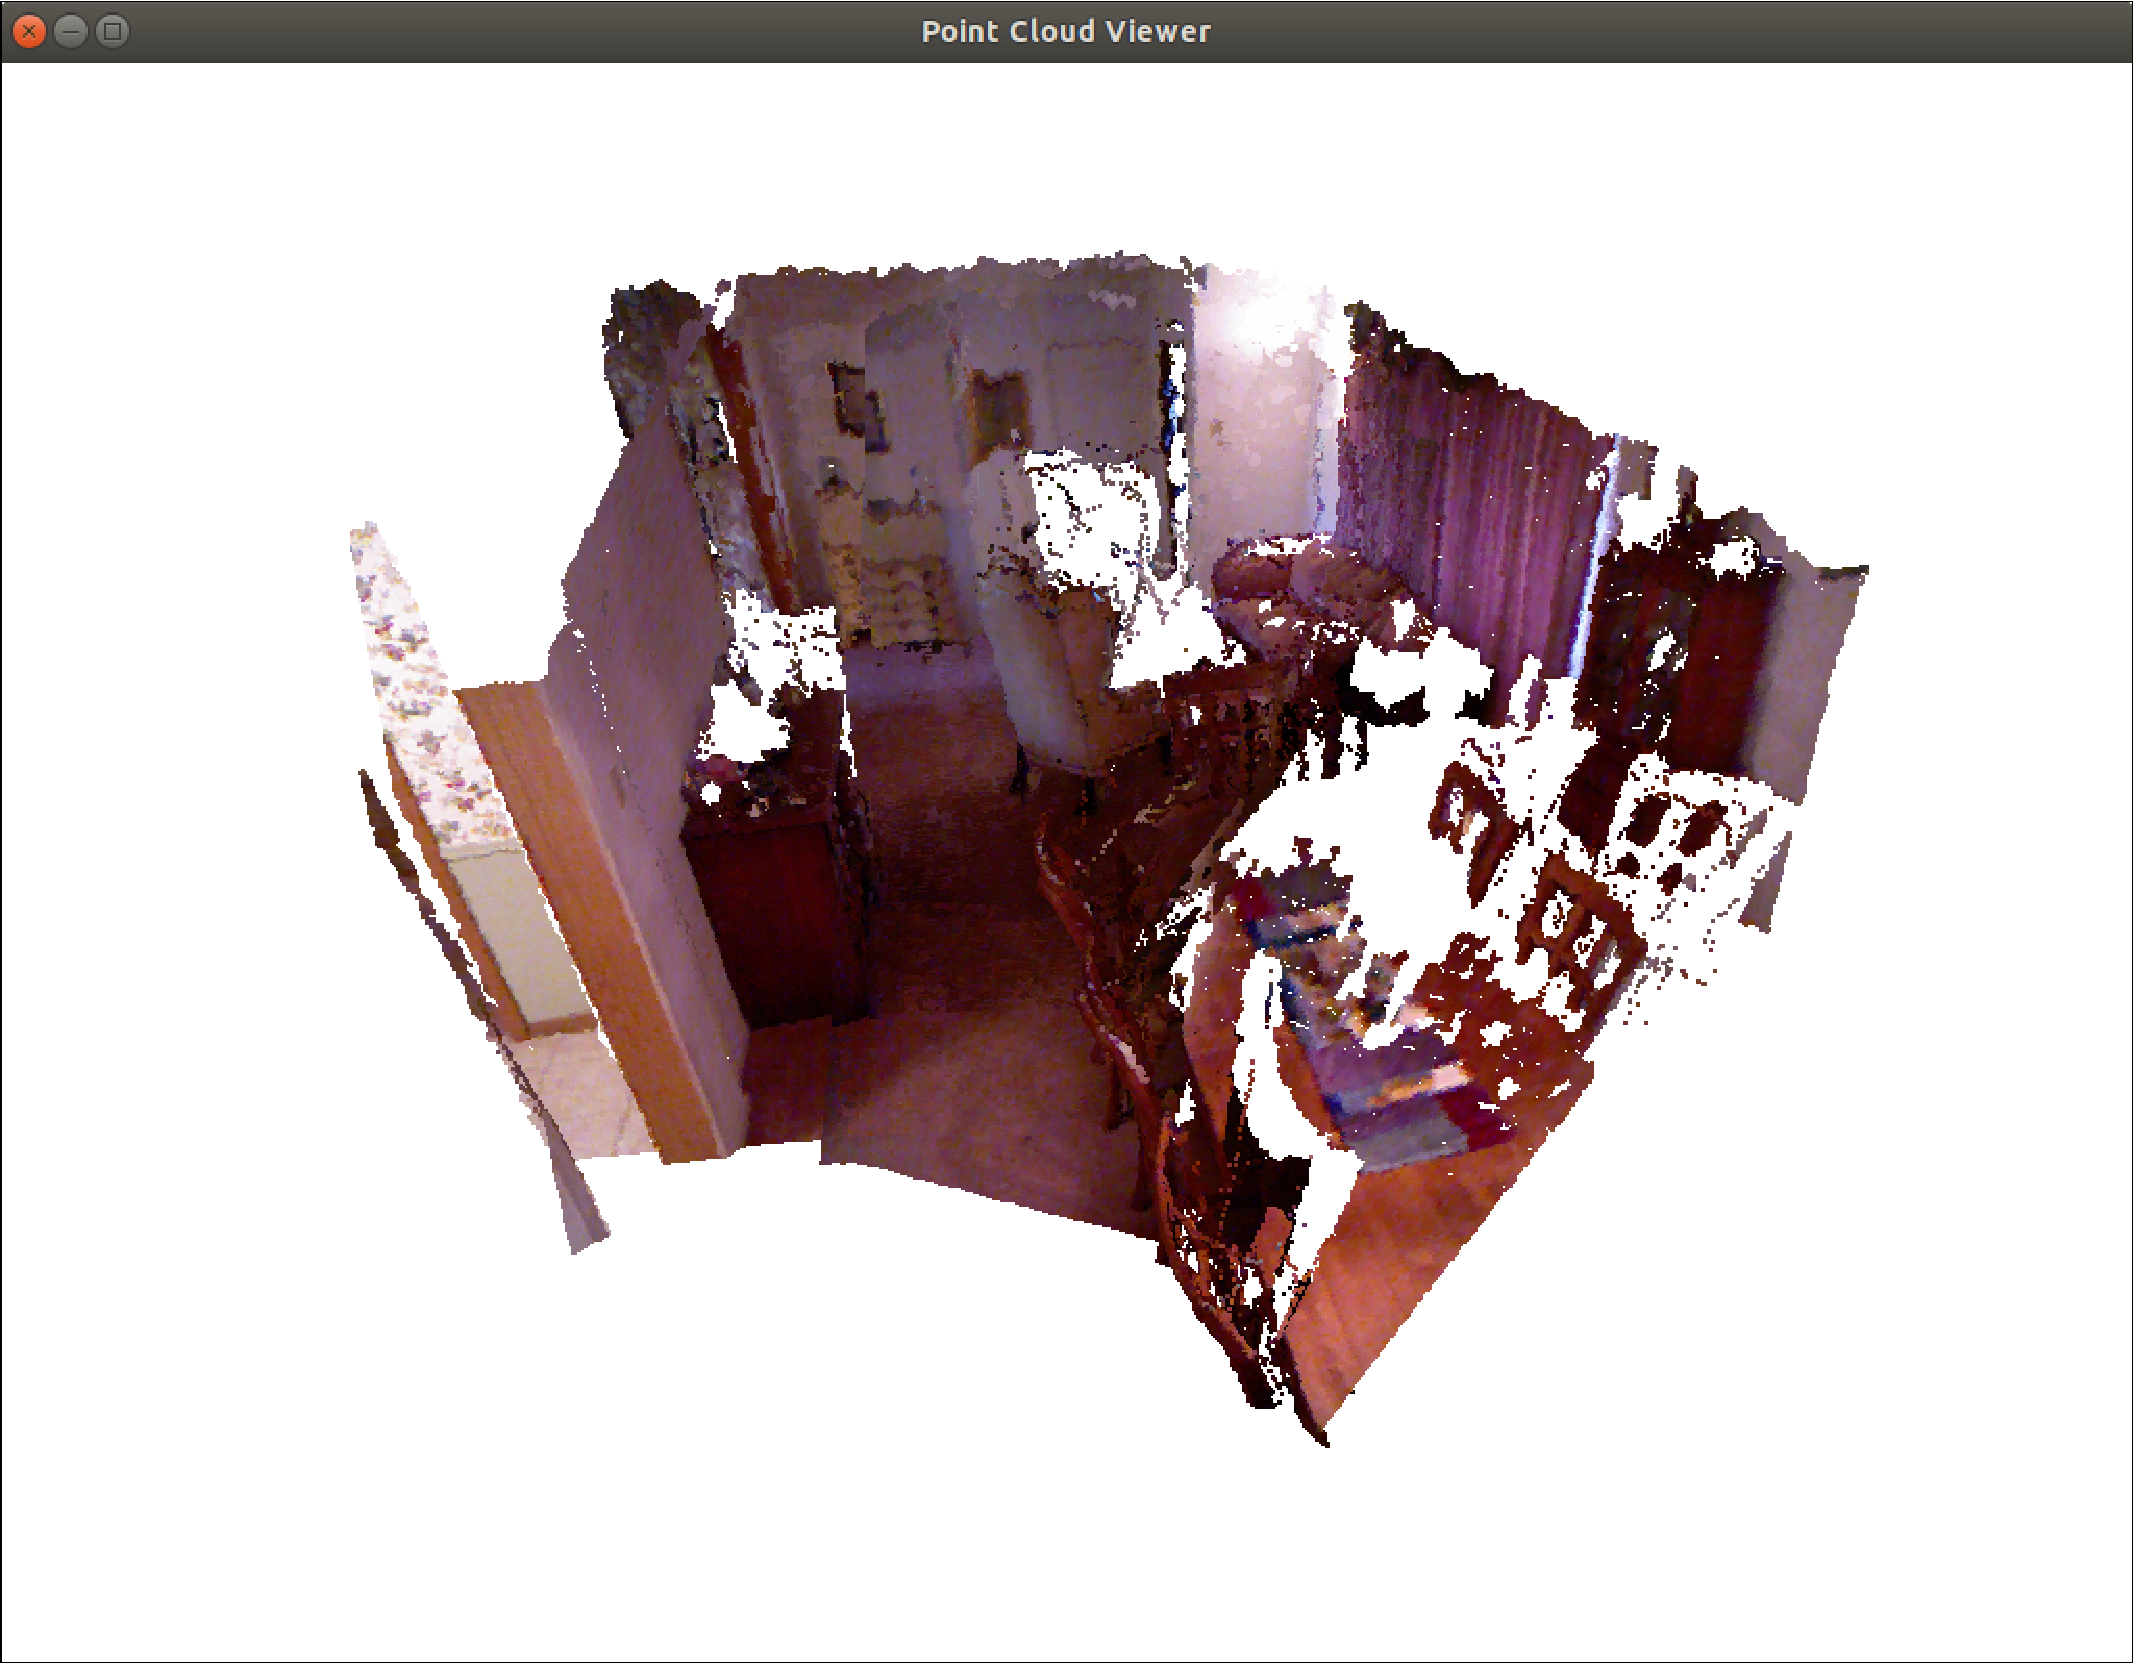
\includegraphics[width=1.0\textwidth]{cameraModel/pointcloud.pdf}
    \caption{The global point cloud from 5 RGBD image pairs.}
    \label{fig:pointcloudmapping}
\end{figure}

We demonstrated some common monocular, binocular, and rgbd camera algorithms in computer vision through these examples. We hope readers can understand the meaning of the intrinsics, extrinsics, and distortion model through them.

\section * {Exercise}
\begin{enumerate}
\item[\optional] Find a camera (use the camera of your mobile phone or laptop if you don't have one) and calibrate its internal parameters. You may use a calibration board or print out a checkerboard for calibration.
\item Describes the physical meaning of the camera's intrinsics. If the resolution of a camera is doubled and the rest is unchanged, how does its intrinsic change?
\item Search for the calibration method of special cameras (fisheye or panoramic cameras). Where are the differences between them and the pinhole models? 
\item Investigate the similarities and differences between a global shutter camera and a rolling shutter camera. What are their advantages and disadvantages in SLAM?
\item How are RGB-D cameras calibrated? Taking Kinect as an example, what parameters need to be calibrated? (Refer to \url{https://github.com/code-iai/iai_kinect2}.)
\item In addition to the way of traversing the image demonstrated by the sample program, what other methods can you give to traverse the image?
\item[\optional] Read the official OpenCV tutorial to learn its basic usage.
\end{enumerate}


% !Mode:: "TeX:UTF-8"
\chapter{Nonlinear Optimization}
\label{cpt:6}
\begin{mdframed}  
	\textbf{Goal of This Chapter}
	\begin{enumerate}[labelindent=0em,leftmargin=1.5em]
		\item Understand how to form the batch state estimation problem into a least square and how to solve the least square problem.
		\item Understand the Gauss-Newton and Levenburg-Marquadt method and implement them.
		\item Learn how to use the Google Ceres and g2o library to solve a least square problem.
	\end{enumerate}
\end{mdframed} 

In the previous lectures, we introduced the motion and observation equations of the classic SLAM model. Now we know that the pose in the equation can be described by the transformation matrix and then optimized by Lie algebra. The observation equation is given by the camera imaging model, in which the internal parameter is fixed with the camera, and the external parameter is the pose of the camera. So, we have figured out the concrete expression of the classic visual SLAM model.

However, due to the presence of noise, the equations of motion and observation can not be exactly met. Although the camera can fit the pinhole model very well, unfortunately, the data we get is usually affected by various unknown noises. Even if we have a high-precision camera and controller, the motion and observations equations can only be approximated. Therefore, instead of assuming that the data must conform to the equation, it is better to estimate the state from the noisy data accurately.

Solving the state estimation problem requires a certain degree of optimization background knowledge. This section will introduce the basic unconstrained nonlinear optimization method and introduce optimization libraries g2o and Ceres.

\newpage
\includepdf{resources/other/ch6.pdf}

\newpage
\section{State Estimation}
\subsection{From Batch State Estimation to Least Square}
According to the previous sections, the SLAM process can be described by a discrete time motion and observation equations like~\eqref{eq:slamproblem}:
\begin{equation}
\left\{ \begin{array}{l}
{\bm{x}_k} = \mathbf{f}\left( {{\bm{x}_{k - 1}},{\bm{u}_k}} \right) + \bm{w}_k\\
{\bm{z}_{k,j}} = \mathbf{h}\left( {{ \bm{y}_j},{ \bm{x}_k}}  \right)+ \bm{v}_{k,j}
\end{array} \right. .
\end{equation}

Through the knowledge in Lecture 4, we learned that $ \bm {x} _k $ is the pose of the camera, which can be described by $ \mathrm {SE} (3) $. As for the observation equation, we have already explained in Lecture 5, the pinhole camera model. In order to give readers a deeper impression of them, we may wish to discuss their specific parameterized form. First, the pose variable $\bm {x} _k $ can be expressed by $\bm {T} _k \in \mathrm {SE} (3) $. Second, the motion is related to the specific form of the input, but there is no particularity in visual SLAM (should be same as the case of ordinary robots and vehicles), we will not talk about it for the time being. The observation equation is given by the pinhole model. Assuming an observation of the road sign $ \bm {y} _j $ at $ \bm {x} _k $, corresponding to the pixel position on the image $ \bm {z} _ {k, j} $, then, observe The equation can be expressed as:
\begin{equation}
s \bm{z}_{k,j}= \bm{K} (\bm{R}_k {\bm{y}_j}+\bm{t}_k),
\end{equation}
where $ \bm {K} $ is the intrinsic matrix of the camera, and $s$ is the distance of pixels, which is also the third element of $ (\bm {R} _k {\bm {y} _j} + \bm {t} _k) $. If we use  transformation matrix $ \bm {T} _k $ to describe the pose, then the points $ \bm {y} _j $ must be described in homogeneous coordinates, and then converted to non-homogeneous coordinates afterwards. If you are not familiar with this process, please go back to the previous lectures.

Now, consider what happens when the data is affected by noise. In the motion and observation equations, we \textbf {usually} assume that the two noise terms $ \bm {w} _k, \bm {v} _ {k, j} $ satisfy a Gaussian distribution with zero mean, like this:
\begin{equation}
{\bm{w}_k} \sim \mathcal{N}\left( {\bm{0},{\bm{R}_k}} \right),{\bm{v}_k} \sim \mathcal{N}\left( {\bm{0},{{{\bm{Q}}}_{k,j}}} \right),
\end{equation}
where $ \mathcal {N} $ means Gaussian distribution, $ \bm{0} $ means zero mean, and $ \bm {R} _k, \bm {Q} _ {k, j} $ is the covariance matrix. Under the influence of these noises, we hope to infer the pose $ \bm {x} $ and the map $ \bm {y} $ from the noisy data $ \bm {z} $ and $ \bm {u} $ (and their probability density distribution), which constitutes a state estimation problem.

There are two ways to deal with this state estimation problem. Since these data come gradually over time in the SLAM process, we should intuitively hold an estimated state at the current moment and then update it with new data. This method is called the \textbf {incremental} method, or \textbf{filtering}. For a long time in history, researchers have used filters, especially the extended Kalman filter (EKF) and its derivatives, to solve it. The other way is to record the data into a file and looking for the best trajectory and map overall time. This method is called the \textbf {batch} estimation. In other words, we can put all the input and observation data from time 0 to $ k $ together and ask, with such input and observation, how to estimate the entire trajectory and map from time 0 to $ k $?

These two different processing methods lead to many different estimation methods. In general, the incremental method only cares about the state estimation of the \textbf {current moment} $ \bm {x} _k $, but does not consider much about the previous state; relatively, the batch method can be used to get an optimized trajectory in larger time or space scope, which is considered to be superior to the traditional filters \textsuperscript {\cite {Strasdat2012}}, and has become the mainstream method of current visual SLAM. In extreme cases, we can let robots or drones collect data and then bring it back to the computing center for unified processing, which is also the mainstream practice of SfM (Structure from Motion). Of course, in these cases, the method is obviously not \textbf {real time}, which is not the most common application scenario of SLAM. So in SLAM, practical methods are usually some compromises. For example, we fix some historical trajectories and only optimize some trajectories close to the current moment, which leads to the \textbf {sliding window estimation} method to be described later.

In theory, the batch method is easier to introduce. At the same time, understanding the batch method also makes it easier to understand the incremental method. Therefore, in this section, we focus on the batch optimization method based on nonlinear optimization, and the Kalman filter and more in-depth knowledge will be discussed in the back-end chapter. Since the batch method is discussed, we will consider all the moments from time 1 to $N$ and assume $M$ map points. Define the robot pose and map coordinates at all times as:
\[
\bm{x}=\{ \bm{x}_1, \ldots, \bm{x}_N \}, \quad \bm{y} = \{\bm{y}_1, \ldots, \bm{y}_M \}.
\]
Similarly, $ \bm {u} $ without subscript is used for input at all times, and $ \bm {z} $ is used for observation data at all times. Then we say that the state estimation of the robot, from a probabilistic point of view, is to find the state $ \bm {x}, \bm{y}$ under the condition that the input data $ \bm {u} $ and the observation data $\bm{z} $. Or, the conditional probability distribution of:
\begin{equation}
P( \bm{x},\bm{y} | \bm{z}, \bm{u}).
\end{equation}

In particular, when we do not know the control input and only have one image, that is, only considering the data brought by the observation equation, it is equivalent to estimating  the conditional probability distribution $ P (\bm {x}, \bm {y} | \bm { z}) $. Such a problem is also called Structure from Motion (SfM), that is, how to reconstruct the three-dimensional spatial structure from images only \textsuperscript {\cite {Agarwal2009}}.

To estimation the conditional pdf we use the Bayes equation to switch the variables:
\begin{equation}
P\left( { \bm{x},\bm{y}| \bm{z}, \bm{u}} \right) = \frac{{P\left( {\bm{z},\bm{u}|\bm{x},\bm{y}} \right)P\left( \bm{x}, \bm{y} \right)}}{{P\left( \bm{z},\bm{u}\right)}} \propto \underbrace{P\left(  { \bm{z},\bm{u}| \bm{x},\bm{y} } \right)}_{\text{likehood}} \underbrace{P\left( \bm{x},\bm{y} \right)}_{\text{prior}}.
\end{equation}

The left side is called \textbf {posterior probability}, and $ P (\bm {z} | \bm {x}) $ on the right is called \textbf {likelihood} (or likehood), and the other part is $ P (\bm {x}) $ is called \textbf {prior}. \textbf {It is normally difficult to find the posterior distribution directly (in nonlinear systems), but it is feasible to find an optimal point which maximize the posterior} (Maximize a Posterior, MAP):
\begin{equation}
{(\bm{x},\bm{y})^*}_{\mathrm{MAP}} = \arg {\mathop{\rm max}\nolimits} P \left( {\bm{x},\bm{y}|\bm{z},\bm{u}} \right) = \arg \max P(\bm{z},\bm{u}|\bm{x},\bm{y})P(\bm{x},\bm{y}).
\end{equation}

Please note that the denominator part of Bayes' rule has nothing to do with the state $ \bm {x}, \bm {y} $ to be estimated, so it can be just ignored. Bayes' rule tells us that solving the maximum posterior probability is \textbf {equivalent to the estimate the product of maximum likelihood and a priori}. Further, we can also say ``I'm sorry, I don't know in prior where the robot pose or the map points are", then there is no \textbf {prior}. Then, you can solve \textbf {Maximize Likelihood Estimation} (MLE):
\begin{equation}
{ (\bm{x},\bm{y})^*}_{\mathrm{MLE}} = \arg \max P( \bm{z},\bm{u}| \bm{x},\bm{y}).
\end{equation}

Intuitively speaking, likelihood refers to ``what observation data may be generated in the current pose''. Since we know the observation data, the maximum likelihood estimation can be understood as: ``\textbf{under what state is it most likely to produce the data currently observed}''. 

\subsection{Introduction to Least Squares}
Now we have a formulated the state estimation problem into a MAP/MLE problem, and the next question is how to solve it. Under the assumption of Gaussian distribution, we can have a simpler form of the maximum likelihood problem. Looking back at the observation model, for a certain kind of observation, we have:
\[
{\bm{z}_{k,j}} = h\left( {{ \bm{y}_j},{ \bm{x}_k}} \right)+ \bm{v}_{k, j},
\]
Since we assume the noise item is gaussian, which means ${\bm{v}_k} \sim \mathcal{N}\left( {\bm{0},{{{\bm{Q}}}_{k,j}}} \right)$, so the conditional probability of the observation data is:
\[
P( \bm{z}_{j,k} | \bm{x}_k, \bm{y}_j) = N\left( h(\bm{y}_j, \bm{x}_k), \bm{Q}_{k,j} \right),
\]
which is, of course, still a Gaussian distribution. Now let's considering to solve the maximum likelihood estimation under this single observation. 

We can rewrite this maximum problem into a \textbf{minimium of negative logarithm} one for Gaussian distributions since they have better mathematical forms under negative logarithm. Consider an arbitrary multi-dimensional Gaussian distribution $\bm{x} \sim \mathcal{N}(\bm{\mu}, \bm{\Sigma})$, its probability density function expansion form is:
\begin{equation}
	P\left( \bm{x} \right) = \frac{1}{{\sqrt {{{(2\pi )}^N}\det (\bm{\Sigma} )} }}\exp \left( {-\frac{1}{2}{{\left( {\bm{x}-\bm{\mu}} \right)}^\mathrm{T}}{ \bm{\Sigma} ^ {-1}}\left( {\bm{x}-\bm{\mu}} \right)} \right).
\end{equation}
Taking the negative logarithm of both sides:
\begin{equation}
	-\ln \left( {P\left( \bm{x} \right)} \right) = \frac{1}{2}\ln \left( {{{\left( {2\pi} \right )}^N}\det \left( \bm{\Sigma} \right)} \right) + \frac{1}{2}{\left( {\bm{x}-\bm{\mu}} \right)^\mathrm{T}}{\bm{\Sigma} ^{-1}}\left( {\bm{x}-\bm{\mu}} \right).
\end{equation}
Because the logarithm function is monotonically increasing, maximizing the original function is equivalent to minimizing the negative logarithm. When minimizing $\bm{x}$ in the above formula, the first term has nothing to do with $\bm{x}$ and can be omitted. Therefore, as long as the quadratic term on the right is minimized, the maximum likelihood estimate of the state is obtained. Substituting into the SLAM observation model, it is equivalent to finding such a solution:
\begin{equation}
	\begin{aligned}
		(\bm{x}_k,\bm{y}_j)^* &= \arg \max \mathcal{N}(h(\bm{y}_j, \bm{x}_k), \bm{Q }_{k,j}) \\ &= \arg \min \left( {{{\left( {{ \bm{z}_{k,j}}-h\left( {{\bm{x }_k},{\bm{y}_j}} \right)} \right)}^\mathrm{T}} \bm{Q}_{k,j}^{-1}\left( {{\ bm{z}_{k,j}}-h\left( {{\bm{x}_k},{\bm{y}_j}} \right)} \right)} \right).
	\end{aligned}
\end{equation}

We found that this equation is equivalent to a quadratic form that minimizes the noise term (i.e., the error). This quadratic form is called \textbf{Mahalanobis distance}. It can also be regarded as the Euclidean distance ($\mathcal{L}_2$-norm) weighted by $\bm{Q}_{k,j}^{-1}$, where $\bm{Q}_{k,j} ^{-1}$ is also called the \textbf{information matrix}, which is extacly the \textbf{inverse} of the Gaussian  \textbf{covariance matrix}.

Now we put all the observations together. It is usually assumed that the inputs and observations at each time are independent of each other, which means that each input is independent, each observation is independent, and input and observation are also independent. So we can factorize the joint distribution like this:
\begin{equation}
	P\left( {\bm{z},\bm{u}|\bm{x},\bm{y}} \right) = \prod\limits_k {P\left( {{\bm{u}_k }|{\bm{x}_{k-1}},{\bm{x}_k}} \right)} \prod\limits_{k,j} {P\left( {{\bm{z} _{k,j}}|{\bm{x}_k},{\bm{y}_j}} \right)},
\end{equation}

It shows that we can handle the movement and observation at each moment independently. Let's define the error between the model and real data: 
\begin{equation}
	\begin{array}{l}
		{\bm{e}_{u,k}} = {\bm{x}_k}-f\left( {{\bm{x}_{k-1}},{\bm{u}_k} } \right)\\
		{\bm{e}_{z,j,k}} = {\bm{z}_{k,j}}-h\left( {{\bm{x}_k},{\bm{y} _j}} \right),
	\end{array}
\end{equation}
Then, minimizing the Mahalanobis distance between the estimated value at all times and the measurements from sensors is equivalent to finding the maximum likelihood estimation. The negative logarithm allows us to turn the product into a summation:
\begin{equation}
	\label{eq:least-square}
	\min J (\bm{x},\bm{y}) = \sum\limits_k {\bm{e}_{u,k}^\mathrm{T} \bm{R}_k^{-1} {\bm{e}_{u,k}}} + \sum\limits_k {\sum\limits_j {\bm{e}_{z,k,j}^\mathrm{T} \bm{Q}_ {k,j}^{-1}{\bm{e}_{z,k,j}}}}.
\end{equation}
In this way, a \textbf{least square problem} is obtained with the same solution as the MLE problem. Intuitively speaking, due to the presence of noise, when we substitute the estimated trajectory and map into the SLAM motion and observation models, they will not be perfectly fit. What shall we do at this time? We perform \textbf{fine-tuning} on the estimated value of the state, so that the overall error is reduced. Of course, finally we will reach a (local) \textbf{minimum value}. This is a typical nonlinear optimization process.

Observing the formula~\eqref{eq:least-square} carefully, we find that the least squares problem in SLAM has some specific structures:

\begin{itemize}
	\item First of all, the objective function of the whole problem consists of many (weighted) error quadratic forms. Although the dimensionality of the overall state variable is very high, each error term is simple and is only related to one or two state variables. For example, the motion error is only related to $\bm{x}_{k-1}, \bm{x}_k$, and the observation error is only related to $\bm{x}_k, \bm{y}_j$. This relationship will give a \textbf{sparse} least square problem, which we will investigate further in the backend chapter.

	\item Secondly, if you use Lie algebra to represent the increment, the problem is the least squares problem of \textbf{unconstrained}. However, if the rotation matrix/transformation matrix is ​​used to describe the pose, the constraint of the rotation matrix itself will be introduced, that is, $\mathrm{s.t.}\ \bm{R}^\mathrm{T} \bm{R} = \bm{I}$ and $\det (\bm{R})=1$ need to be added to the problem. Additional constraints can make optimization more difficult.

	\item Finally, we used a quadratic metric error, which is exactly the $\mathcal{L}_2-$norm. The information matrix is used as the weights of each elemnents. For example, if an observation is very accurate, the covariance matrix will be ``small'' and the information matrix will be ``large'', so this error term will have a higher weight than the others in the whole problem. We will see some drawbacks of the $\mathcal{L}_2$ error later.
\end{itemize}

We introduce how to solve this least-squares problem, which requires some \textbf{basic knowledge of nonlinear optimization}. In particular, we want to discuss how to solve such a general unconstrained nonlinear least-squares problem. In the following lectures, we will make extensive use of this lecture's results and discuss in detail its application in the front and back ends of SLAM.

\subsection{Example: Batch state estimation}
Maybe it's better to give an example here. Consider a very simple discrete-time system:
\begin{equation}
    \begin{array}{lll}
        {x_k} &= {x_{k-1}} + {u_k} + {w_k},&\qquad w_k \sim \mathcal{N}\left( {0,Q_k} \right)\\
        {z_k} &= {x_k} + {n_k},&\qquad {n_k}\sim \mathcal{N}\left( {0,R_k} \right)
    \end{array},
\end{equation}
which can express a car moving forward or backward along the $x$ axis. The first formula is the motion model, where $u_k$ is the input, and $w_k$ is the noise; the second formula is the observation model, where $z_k$ is the measurement of the car position. We set the time $k=1,\ldots,3$, and want to estimate the states based on the existing $v,y$. Suppose the initial state $x_0$ is known. Let's derive the maximum likelihood estimation of the batch state estimation.

First, let the batch state variable be $\bm{x} = [x_0,x_1, x_2, x_3]^\mathrm{T}$, and the batch observation be $\bm{z} = [z_1,z_2,z_3]^ \mathrm{T}$, define $\bm{u}=[u_1,u_2,u_3]^\mathrm{T}$ in the same way. According to the previous derivation, we know that the maximum likelihood estimate is:
\begin{equation}
    \begin{aligned}
        {\bm{x}_{\mathrm{map}}^*} &= \arg \max P(\bm{x}|\bm{u},\bm{z}) = \arg \max P( \bm{u},\bm{z}|\bm{x})\\
        &= \prod\limits_{k = 1}^3 {P({u_k}|{x_{k-1}},{x_k})\prod\limits_{k = 1}^3 {P\left( { {z_k}|{x_k}} \right)} },
    \end{aligned}
\end{equation}
For each item, such as the equation of motion, we have:
\begin{equation}
    P({u_k}|{x_{k-1}},{x_k}) = \mathcal{N}({x_k}-{x_{k-1}},{Q_k}).
\end{equation}
The observation equation is similar:
\begin{equation}
    P\left( {{z_k}|{x_k}} \right) = \mathcal{N}\left( {{x_k},{R_k}} \right).
\end{equation}

According to the previous statements, the error variable can be constructed as:
\begin{equation}
    {e_{u,k}} = {x_k}-{x_{k-1}}-{u_k}, \quad {e_{z,k}} = {z_k}-{x_k},
\end{equation}
Then the objective function of least squares is:
\begin{equation}
    \min \sum\limits_{k = 1}^3 {e_{u,k}^\mathrm{T} Q_k^{-1}{e_{u,k}}} + \sum\limits_{k = 1 }^3 {e_{z,k}^\mathrm{T}{R^{-1}_k}{e_{z,k}}}.
\end{equation}

In addition, since this system is a linear one, we can easily write the equations in vector/matrix form. Define the vector $\bm{y}=[\bm{u}, \bm{z}]^\mathrm{T}$, then the error can be defined as: 
\begin{equation}
    \bm{y}-\bm{H}\bm{x} = \bm{e} \sim \mathcal{N}(\bm{0}, \boldsymbol{\Sigma}),
\end{equation}
where
\begin{equation}
    \bm{H} = \left[ {\begin{array}{*{20}{c}}
            1&{-1}&0&0\\
            0&1&{-1}&0\\
            0&0&1&{-1}\\
            \hline
            0&1&0&0\\
            0&0&1&0\\
            0&0&0&1
    \end{array}} \right],
\end{equation}
and $\boldsymbol{\Sigma}=\mathrm{diag}(Q_1, Q_2, Q_3, R_1, R_2, R_3)$. The whole question can be written as:
\begin{equation}
    \bm{x}^*_{\mathrm{map}} = \arg \min \bm{e}^\mathrm{T} \boldsymbol{\Sigma}^{-1} \bm{e},
\end{equation}
Later we will see that this problem has a unique solution:
\begin{equation}
    \bm{x}^*_{\mathrm{map}} = (\bm{H}^\mathrm{T} \boldsymbol{\Sigma}^{-1} \bm{H})^{-1} \bm{H}^\mathrm{T} \boldsymbol{\Sigma}^{-1} \bm{y},
\end{equation}
since the $(\bm{H}^\mathrm{T} \boldsymbol{\Sigma}^{-1} \bm{H})^{-1}$ is invertible.

\section{Nonlinear least squares}
\label{sec:6.2}
First consider a simple least squares problem:
\begin{equation}
    \mathop {\min }\limits_{\bm{x}} F(\bm{x}) = \frac{1}{2}{\left\| {f\left( \bm{x} \right) } \right\|^2_2}.
\end{equation}

Among them, the status variable is $\bm{x} \in \mathbb{R}^n$, and $f$ is any scalar nonlinear function $f(\bm{x}): \mathbb{R}^n \mapsto \mathbb{R}$. Note that the coefficient $\frac{1}{2}$ here is not important, some literature have this coefficient and some not. It will not affect the subsequent conclusions. Obviously, if $f$ is a mathematically simple function, then the problem can be solved in analytical form. Let the derivative of the objective function be zero, and then find the optimal value of $\bm{x}$, just like finding the extreme value of a scalar function:
\begin{equation}
    \frac{ \mathrm{d} F}{ \mathrm{d} \bm{x}} = \bm{0}.
\end{equation}

We reach the minimum, maximum, or saddle points by solving this equation (or, intuitively, by letting the derivative be zero). But is this equation easy to solve? Well, it depends on the form of the derivative function of $f$. If $f$ is just a simple linear function, then the problem is only a simple linear least squares problem. Still, some derivative functions may be complicated in form, making the equation difficult to solve. Solving this equation requires us to know the \textbf{global property} of the objective function, which is usually not possible. For the least squares problem that is inconvenient to solve directly, we can use \textbf{iterated methods} to start from an initial value and continuously update the current estimations to reduce the objective function. The specific steps can be listed as follows:

\begin{mdframed}  
    \begin{enumerate}
        \item Give an initial value $\bm{x}_0$.
        \item For $k$-th iteration, we find an incremental value of $\Delta \bm{x}_k$, such that the object function $\left\| {f\left( \bm{x}_k + \Delta \bm{x}_k \right)} \right \|^2_2$ reaches a smaller value.
        \item If $\Delta \bm{x}_k$ is small enough, stop the algorithm.
        \item Otherwise, let $\bm{x}_{k+1} = \bm{x}_k+\Delta \bm{x}_k$ and return to step 2.
    \end{enumerate}
\end{mdframed}

Now things get much simpler. We turn the problem of solving \textbf{the derivative function equals zero} into a problem of \textbf{looking for decreasing increments} $\Delta \bm{x}_k$. We will see that since the objective function can be linearly approximated at the current estimation, the increment calculation will be simpler \footnote{Linear cases are always the easiest ones.}. When the function decreases until the increment becomes very small, it is considered that the algorithm converges, and the objective function reaches a minimum value. In this process, the problem is how to find the increment at each iteration point, which is a local problem. We only need to be concerned about the local properties of $f$ at the iteration value rather than the global properties. Such methods are widely used in optimization, machine learning, and other fields.

Next, we examine how to find this increment $\Delta \bm{x}_k$. This part of knowledge belongs to the field of numerical optimization. Let's take q quick look at some of the widely used results.

\subsection{First and Second-order Method}
Now consider the $k$-th iteration. Suppose we are at $\bm{x}_k$ and want to find the increment $\Delta \bm{x}_k$, then the most intuitive way is to make the Taylor expansion of the objective function in $\bm{x}_k$:
\begin{equation}
    F(\bm{x}_k+\Delta \bm{x}_k) \approx F{\left( \bm{x}_k \right)} + \bm{J} \left( \bm{x}_k \right) ^\mathrm{T} \Delta \bm{x}_k + \frac{1}{2}\Delta {\bm{x}_k^\mathrm{T}}\bm{H}(\bm{ x}_k) \Delta \bm{x}_k,
\end{equation}
where $\bm{J}(\bm{x}_k)$ is the first derivative of $F(\bm{x})$ with respect to $\bm{x}$ (also called gradient, \textbf{Jacobi} Matrix, or \textbf{Jacobian}) \footnote{We write $\bm{J}(\bm{x})$ as a column vector, then it can be inner product with $\Delta \bm{x}$ to get a scalar. }, $\bm{H}$ is the second-order derivative (or \textbf{Hessian}), which are all taken at $\bm{x}_k$. Readers should be familiar with them in the undergraduate course like multivariate calculus. We can choose to keep the first-order or second-order terms of the Taylor expansion, and the corresponding solution is called the first-order or the second-order method. In the simplest way, if we only keep the first-order one, then taking the increment at the minus gradient direction will ensure that the function decreases: 
\begin{equation}
    \Delta \bm{x}^* =-\bm{J}(\bm{x}_k).
\end{equation}

Of course, this is only a direction, usually we have to compute another step length parameter, say, $\lambda$. The step length can be calculated according to certain conditions \textsuperscript{\cite{Wolfe1969}}. There are also some empirical methods in machine learning, but we will not discuss them. This method is called \textbf{steepest descent method}. Its intuitive meaning is very simple, as long as we move along the reverse gradient direction, the objective function must decrease if the first-order (linear) approximation still holds.

Note that the above discussion was carried out during the $k$-th iteration and did not involve any information about $k$. To simplify the notation, we will omit the subscript $k$ later and think that these discussions are valid for any iterations.

On the other hand, we can choose to keep the second step information, and the increment equation is:
\begin{equation}
    \Delta \bm{x}^* = \arg \min \left(F\left( \bm{x} \right) + \bm{J} \left( \bm{x} \right)^\mathrm{ T} \Delta \bm{x} + \frac{1}{2}\Delta {\bm{x}^\mathrm{T}}\bm{H} \Delta \bm{x} \right).
\end{equation}
The right side only contains the zero-order, first-order and quadratic terms of $\Delta \bm{x}$. Finding the derivative of $\Delta \bm{x}$ on the right side of the equation and setting it to zero leads to: \footnote{For students who are not familiar with matrix derivation, please refer to Appendix B. }
\begin{equation}
    \label{eq:newton-method}
    \bm{J} + \bm{H} \Delta \bm{x} = \bm{0} \Rightarrow
    \bm{H} \Delta \bm{x} = -\bm{J}.
\end{equation}

We can also solve this linear equation and get the increment. This method is also called \textbf{Newton's method}.

We have seen that both the first-order and second-order methods are very intuitive, as long as we can calculate Taylor expansion of $f$ and find the increments. We say, hey, the function looks like a linear or quadratic one. We can use the approximated function's minimum value to guess the minimum value of the original function. As long as the original objective function really looks like a first-order or quadratic function locally, this type of algorithm is always valid (this is also most cases in reality). However, these two methods also have their drawbacks. The steepest descent method is too greedy and easy to lead a zigzag way and increases the number of iterations. However, Newton's method needs to calculate the $\bm{H}$ matrix of the objective function, which is very time-expensive when the problem is large, and we usually tend to avoid the calculation of $\bm{H}$. For general problems, some quasi-Newton methods can get better results, and for least squares problems, there are several more practical methods: the \textbf{Gauss-Newton's method} and the (Levernburg-Marquardt's method).

\subsection{The Gauss-Newton Method}
The Gauss-Newton method is one of the simplest methods in optimization algorithms. Its idea is to carry out a first-order Taylor expansion of $f(\bm{x})$. Please note that this is not the objective function $F(\bm{x})$ but the lower case $f(\bm{x})$, otherwise it is same as the Newton's method.
\begin{equation}
    \label{eq:approximation}
    f\left( {\bm{x} + \Delta \bm{x}} \right) \approx f\left( \bm{x} \right) + \bm{J} \left( \bm{x} \right)^\mathrm{T} \Delta \bm{x}.
\end{equation}

Here $\bm{J}(\bm{x})$ is the derivative of $f(\bm{x})$ with respect to $\bm{x}$, which is a column vector of $n \times 1$. According to the previous framework, the current goal is to find the increment $\Delta \bm{x}$ such that $\left\| {f\left( \bm{x} + \Delta \bm{x} \right)} \right \|^2$ reached the minimum. In order to find $\Delta \bm{x}$, we need to solve a linear least square problem:
\begin{equation}
    \Delta \bm{x}^* = \arg \mathop {\min }\limits_{\Delta \bm{x}} \frac{1}{2}{\left\| {f\left( \bm{x} \right) + \bm{J} \left( \bm{x} \right)^\mathrm{T} \Delta \bm{x} } \right\|^2}.
\end{equation}
    
What's the difference from before? According to the extreme conditions, we set the derivative with $\Delta \bm{x}$ to zero to reach the extreme value. To do this, let's first expand the square term of the objective function:
\begin{align*}
    \frac{1}{2}{\left\| {f\left( \bm{x} \right) + \bm{J} \left( \bm{x} \right)^\mathrm{T} \Delta \bm{x}} \right\|^2} &= \frac{1}{2}{\left( {f\left( \bm{x} \right) + \bm{J}\left( \bm{x} \right)^\mathrm{T} \Delta \bm{x}} \right)^\mathrm{T}}\left( {f\left( \bm{x} \right) + \bm{J} \left( \bm{x} \right)^\mathrm{T} \Delta \bm{x}} \right)\\
    &= \frac{1}{2}\left( \| f{{\left( \bm{x} \right)}\|^2_2 + 2 f\left( \bm{x} \right) \bm{J} {{\left( \bm{x} \right)}}^\mathrm{T} \Delta \bm{x} + \Delta { \bm{x}^\mathrm{T}}{\bm{J} (\bm{x})} \bm{J}(\bm{x})^\mathrm{T} \Delta \bm{x}} \right).
\end{align*}


Find the derivative of the above formula with respect to $\Delta \bm{x}$ and set it to zero:
\begin{displaymath}
    \bm{J} {\left( \bm{x} \right)}f\left( \bm{x} \right) + \bm{J} {\left( \bm{x} \right)} \bm{J}^\mathrm{T} \left( \bm{x} \right)\Delta \bm{x} = \bm{0}.
\end{displaymath}

The following equations can be obtained:
\begin{equation}
    \underbrace{\bm{J} {\left( \bm{x} \right)} \bm{J}^\mathrm{T}}_{\bm{H}(\bm{x})} \left( \bm{x} \right)\Delta \bm{x} =  \underbrace{- \bm{J} {\left( \bm{x} \right)} f\left( \bm{x} \right)}_{\bm{g}(\bm{x})}.
\end{equation}

This equation is a \textbf{linear equation} of the variable $\Delta \bm{x}$. We call it \textbf{normal equation} or \textbf{Gauss-Newton equation}. We define the coefficients on the left as $\bm{H}$ and the coefficient on the right as $\bm{g}$, then the above formula becomes:
\begin{equation}
    \label{eq:minimize-deltax}
    \bm{H} \Delta \bm{x} = \bm{g}.
\end{equation}
It makes sense to mark the left side as $\bm{H}$ here. Compared with Newton's method~\ref{eq:newton-method}, Gauss-Newton's method uses $\bm{J}\bm{J}^\mathrm{T}$ \textbf{as the approximation} of the second-order Hessian matrix in Newton's method, thus omitting the calculation of $\bm{H}$. Please note that solving the normal equation is the core of the entire optimization problem. If we can get the $\Delta \bm{x}$ in each iteration, then the algorithm of Gauss-Newton method can be written as:

\begin{mdframed}
    \begin{enumerate}
        \item Set it initial value as $\bm{x}_0$.
        \item For $k$-th iteration,calculate the Jacobian $\bm{J}(\bm{x}_k)$ and residual $f(\bm{x}_k)$.
        \item Solve the normal equation: $\bm{H} \Delta \bm{x}_k = \bm{g}$.
        \item If $\Delta \bm{x}_k$ is small enough, stop the algorithm. Otherwise let $\bm{x}_{k+1} = \bm{x}_k+\Delta \bm{x}_k$ and return to step 2.
    \end{enumerate}
\end{mdframed}

It can be seen from the algorithm steps that the solution of the incremental equation occupies a major position. As long as we can solve the increment smoothly, we can ensure that the objective function decreases correctly.

In order to solve the incremental equation, we need to solve $\bm{H}^{-1}$, which requires the $\bm{H}$ matrix to be invertible, but the calculated $\bm{J} \bm{ J}^\mathrm{T}$ is only semi-positive definite. If $\bm{J}$ has null-spaces, which is to say, we can find non-zero $\Delta \bm{x}$ such that $\bm{J} \Delta\bm{x} = \bm{0}$, then we can not determine which $\Delta \bm{x}$ can really makes the objective function really decreases. In that cases, the algorithm is probably not converging and we may obtain erroneous results. Intuitively, the local approximation of the original function at this point is not like a quadratic function. Furthermore, even if we assume that $\bm{H}$ is not singular or ill-conditioned, but if we take a very large step size $\Delta \bm{x}$, the result can still be bad since linear approximation is not accurate enough at that point. So in practice, we can't guarantee that the Gauss-Newton method converges. Sometimes they can reach even larger objective functions values that the initial one. 

Although the Gauss-Newton method has these shortcomings, it is still a simple and effective method for nonlinear optimization, and it is worth learning. In nonlinear optimization, quite a few algorithms can be taken as the variants of the Gauss-Newton method. These algorithms all use the idea of the Gauss-Newton method and correct their shortcomings through their own improvements. For example, some \textbf{line search method} adds an extra step size $\alpha$. After determining $\Delta \bm{x}$, we may further find the $\alpha$ to make $\left\| f (\bm{x} + \alpha \Delta \bm{ x}) \right\|^2$ is minimized, instead of simply making $\alpha = 1$.

The Levenberg-Marquardt method corrects these problems to a certain extent. It is generally considered to be more robust than the Gauss-Newton method, but its convergence rate may be slower than the Gauss-Newton method, and is called \textbf{damped Newton Method}.


% !Mode:: "TeX:UTF-8"
\chapter{Visual Odometry: Part I}
\label{cpt:7}
\thispagestyle{empty}

\begin{mdframed}  
	\textbf{Goal of Study}
	\begin{enumerate}[labelindent=0em,leftmargin=1.5em]
		\item Study how to extract feature points from images and match feature points in multiple images.
		\item Learn the principle of epipolar geometry and use epipolar constraints to recover the camera's 3D motion between two images.
		\item Study how to solve the PNP problem and use the known correspondence between the 3D structure and the 2D image to solve the camera's 3D motion.	
		\item Study the ICP algorithm and use the point clouds matching to estimate 3D motion.
		\item Study how to obtain the 3D structure of corresponding points on the 2D image through triangulation.
	\end{enumerate}
\end{mdframed}

In the previous chapters, we introduced the details of motion and observation equations and explained how nonlinear optimization is used to solve those equations. From this chapter, we finish introducing the fundamental knowledge and moving on to the next topic. Starting from this chapter, we will investigate visual odometry, backend optimization, loop detection, and map reconstruction. This chapter and the next chapter mainly focus on two commonly used visual odometry methods: the feature and direct methods. This chapter will introduce what feature points are, how to extract and match them, and how to estimate camera motion based on matched feature points.

\newpage
\includepdf{resources/other/ch7.pdf}

\newpage

\section{Feature Method}
In chapter \ref{cpt:2}, we said that a SLAM system can be divided into frontend and backend, where the frontend is also called visual odometry (VO). VO estimates the rough camera movement based on the consecutive images' information and provides a good initial value for the backend. VO algorithms are mainly divided into two categories: feature method and direct method. The frontend based on the features has been considered the mainstream of VO for a long time (even until now). It performs well thanks to its stability and insensitivity to lighting and dynamic objects. The feature method is relatively mature at present. This chapter will start with the feature method, learn how to extract and match image feature points, and then estimate the camera motion and scene structure between two frames to realize visual odometry between two frames. This type of algorithm is sometimes called two-view geometry.

The core problem of VO is how to estimate camera motion based on adjacent images. However, the image itself is a numerical matrix encoding brightness and color. The numbers in the matrix are abstract, and it is very difficult to compute the motion directly from the pixel level. Therefore, it is more convenient to do this: First, select some representative features from the image. These points will remain the same after a small change in the camera's angle of view. So we are able to find the same points in each image. Then, based on these points, we can investigate the problem of camera pose estimation and the 3D positions of these points. In the classic SLAM model, we call these points the landmarks. In visual SLAM, they are referred to as image features.

On Wikipedia, image features are defined as a set of information related to computing tasks. The computing tasks depend on the specific application {\cite{wiki:featurecv}}. Briefly speaking, the feature is another digital expression of image information. A good set of features is crucial to the final performance on the specified task, so researchers have comprehensive work on the features for many years. Digital images are stored in a computer as a gray value matrix, so at the simplest, a single image pixel can also be considered a feature. However, in visual odometry, we hope that feature points remain stable after the camera moves, and the gray value is severely affected by illumination, deformation, and object material. It varies significantly between different images and is not stable enough. Ideally, when the scene and camera angle of view changes slightly, the algorithm can also determine from the images which places refer to the same point. Therefore, the gray value alone is not feasible. We need to extract better features from the image.

We can say that the feature points are some special places in the image. Taking \autoref{fig:corner-feature}~ as an example, we can see the corners, edges, and blocks as representative places in the image. It is easy for us to correctly point out that the same corner point appears in two images, whereas pointing out the same edge is slightly more difficult because the image patches are similar when moving along the edges. It is even harder for the blocks. We found that the corners and edges in the image are more \textit{special} than pixels, and they are more distinguished between different images. Therefore, an intuitive way to extract features is to identify corners between different images and determine their correspondence. In this approach, the corners are the so-called features. There are many corner extraction algorithms, such as Harris corner {\cite{Harris1988}}, FAST corner {\cite{Rosten2006}}, GFTT corner  {\cite{Shi1994}}, etc. Most of them were proposed before 2000.

However, in the majority of applications, a single corner still cannot meet our needs. For example, a place that appears to be a corner from a long distance may not be viewed as a corner when the camera steps in. When the camera rotates, the appearance of the corner points will change, and it is not easy for us to recognize that they are the same corner point. For this reason, researchers in the field of computer vision have designed many more stable local image features during years of research, such as the SIFT {\cite{Lowe2004}}, SURF {\cite{Bay2006}} , ORB {\cite{Rublee2011}}, etc. Compared with simple corner points, these handcrafted features should have the following properties:

\begin{enumerate}
\item \textbf{Repeatability}: The same feature can be found in different images.
\item \textbf{Distinctiveness}: Different features have different expressions.
\item \textbf{Efficiency}: In the same image, the number of feature points should be far smaller than the number of pixels.
\item \textbf{Locality}: The feature is only related to a small image area.
\end{enumerate}

\begin{figure}[!ht]
    \centering
    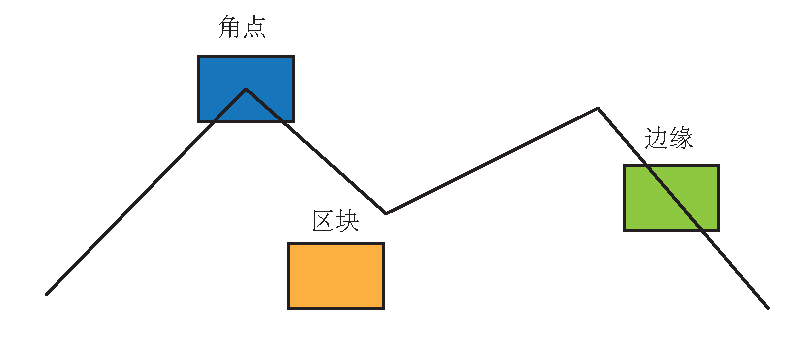
\includegraphics[width=0.8\linewidth]{vo1/corner-flat-line}
    \caption{Corners, edges and blocks can be used as image features.}
    \label{fig:corner-feature}
\end{figure}

A feature point is composed of two parts: \textit{key point} and \textit{descriptor}. For example, when we say ``calculate SIFT feature points in an image'', we mean ``extract SIFT key points and calculate the SIFT descriptors``. The key point refers to the 2D position of the feature point. Some types of key points also hold other information, such as the orientation and size. According to some handcrafted rules, the descriptor is usually a vector, describing the information of the pixels around the key point. The descriptor should be designed according to the principle that features with similar appearance should have similar descriptors. Therefore, as long as the two features' descriptors are close in vector space, they can be considered the same feature. 

Historically, researchers put forward many image features. Some of them are very accurate and robust. They still have similar expressions under camera movement and lighting changes, and consequentially they might require a large amount of calculation. Among them, SIFT (Scale-Invariant Feature Transform) is one of the most classic. To fully consider the changes in illumination, scale, and rotation during the image transformation, the SIFT comes with a considerable amount of calculation. The extraction and matching of image features is only a part compared to the entire SLAM process. Until now (2016), CPUs equipped on PCs cannot achieve real-time to calculate the SIFT features for localization and mapping \footnote{Real-time means the speed of 30Hz. }. So, we rarely use this luxury image feature in SLAM.

Some other features exchange accuracy and robustness for the calculation speed increase. For example, the FAST keypoint is a key point that is extremely fast to calculate (note the expression of keypoint here, which means that it has no descriptor), while the ORB (Oriented FAST and Rotated BRIEF) feature is currently widely used for real-time image feature extraction. It solves the problem that the FAST detector  {\cite{Rosten2006}} does not have descriptors and uses the extremely fast binary descriptor BRIEF {\cite{calonder2010brief}} to make the whole image feature extraction process accelerate greatly. According to the author's experiment in the paper, extracting about 1000 feature points in the same image takes about 15.3ms for ORB, 217.3ms for SURF, and 5228.7ms for SIFT. It can be seen that ORB made a significant boost in speed while maintaining the features of rotation and scale invariance. It is a good choice for SLAM with high real-time requirements.

Most feature extractions have good parallelism and can be accelerated by GPU and other devices. SIFT accelerated by GPU can meet real-time requirements. However, the inclusion of a GPU will increase the cost of the entire SLAM system \footnote{But now we have many cheap embedded GPU chips, so it may not be an issue anymore.}. Whether the resulting performance improvement is sufficient to offset the computational cost requires careful consideration by the system designer.

Obviously, there are a large number of feature points in the field of computer vision, and we cannot introduce them one by one in the book. In the current SLAM scheme, ORB is a fair trade-off between quality and performance. Therefore, we take ORB as an example to introduce the entire process of extracting features. If readers are interested in feature extraction and matching algorithms, we recommend reading related books in this area \cite{Nixon2012}.

\subsection{ORB Feature}

ORB features are also composed of two parts: \textit{ORB key points} and \textit{ORB descriptor}. Its key point is called ``oriented FAST'', which is an improved version of the FAST. We will introduce what the FAST corner below is. Its descriptor is called BRIEF (Binary Robust Independent Elementary Feature). Therefore, the extraction of ORB features is divided into the following two steps:
\begin{enumerate}
\item FAST corner point extraction: find the corner point in the image. Compared with the original FAST, the main direction of the feature points is calculated in ORB, making the subsequent BRIEF descriptor rotation-invariant.
\item BRIEF descriptor: describe the surrounding image area where the feature points were extracted in the previous step. ORB has made some improvements to BRIEF, mainly referring to utilizing the previously calculated direction.
\end{enumerate}

Next, we will introduce FAST and BRIEF, respectively.

\subsubsection{The FAST Key Point}
FAST is a kind of corner point, which mainly detects the local grayscale changes and is known for its fast speed. Its main idea is: if a pixel is very different from the neighboring pixels (too bright or too dark), it is more likely to be a corner point. Compared with other corner detection algorithms, FAST only needs to compare the pixels' brightness. Its entire procedure is as follows (see \autoref{fig:fastcorner}~):

\begin{enumerate}
\item Select pixel $p$ in the image,assuming its brightness as $I_{p}$
\item Set a threshold $T$ (for example, 20\% of $I_{p}$).
\item Take the pixel $p$ as the center, and select the 16 pixels on a circle with a radius of 3.
\item If there are consecutive $N$ points on the selected circle whose brightness is greater than $I_{p}+T$ or less than $I_{p}-T$, then the central pixel $p$ can be considered a feature point. $N$ usually takes 12, which is FAST-12. Other commonly used $N$ values ​​are 9 and 11, called FAST-9 and FAST-11, respectively).
\item Iterate through the above four steps on each pixel.
\end{enumerate}

In the FAST-12 algorithm, to speed up, we can check the brightness of the 1, 5, 9, and 13 pixels on the circle to quickly exclude many pixels that are not corner points. Only when three of these four pixels are all greater than $I_{p}+T$ or less than $I_{p}-T$, the current pixel may potentially be a corner point. Otherwise, it should be directly excluded. Such a pre-processing operation greatly accelerates FAST corner detection. Also, the original FAST corners are often clustered, meaning a lot of FAST corners may present in the same area. Therefore, after the initial detection, non-maximal suppression is required. Only corner points with the maximum response in a specific location will be retained to avoid the corners concentrating.

\begin{figure}[!ht]
	\centering
	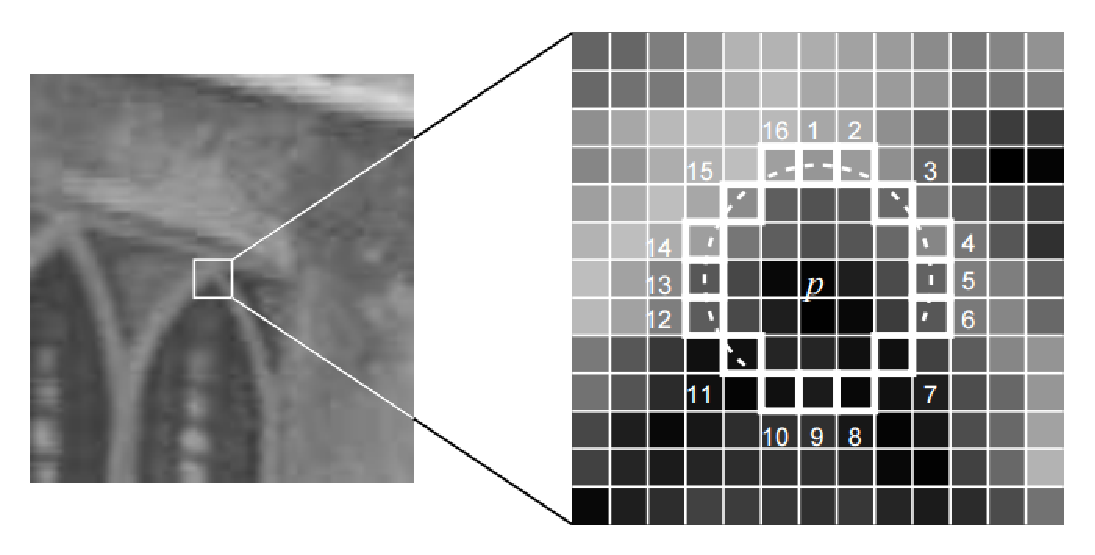
\includegraphics[width=0.9\linewidth]{vo1/fast-corner}
	\caption{FAST key points {\cite{Rosten2006}}. This figure is from OpenCV's document.}
	\label{fig:fastcorner}
\end{figure}

The calculation of FAST feature points only compares the brightness difference between pixels, thus the speed is very fast, but it suffers from lousy repeatability and uneven distribution. Moreover, FAST corner points do not include direction information. Because it fixed the radius of the circle as 3, there is also a scaling problem: a place that looks like a corner from a distance may not be a corner when it comes close. To solve those, ORB adds the description of scale and rotation. The scale invariance is achieved by the image pyramid \footnote{Pyramid refers to the downsampling of images at different levels to obtain images with different resolutions. } and detect corner points on each layer. The rotation of features is realized by the intensity centroid method.

An image pyramid is a common approach in computer vision. For a schema, see \autoref{fig:pyramid}. The bottom of the pyramid is the original image. For each layer up, the image is scaled with a fixed ratio so that we have images of different resolutions. The smaller image can be seen as a scene viewed from a distance. In the feature matching algorithm, we can match images on different layers to achieve scale invariance. For example, if the camera moves backward, we should find a match in the upper layer of the previous image pyramid and the lower layer of the next image.

\begin{figure}[!t]
    \centering
    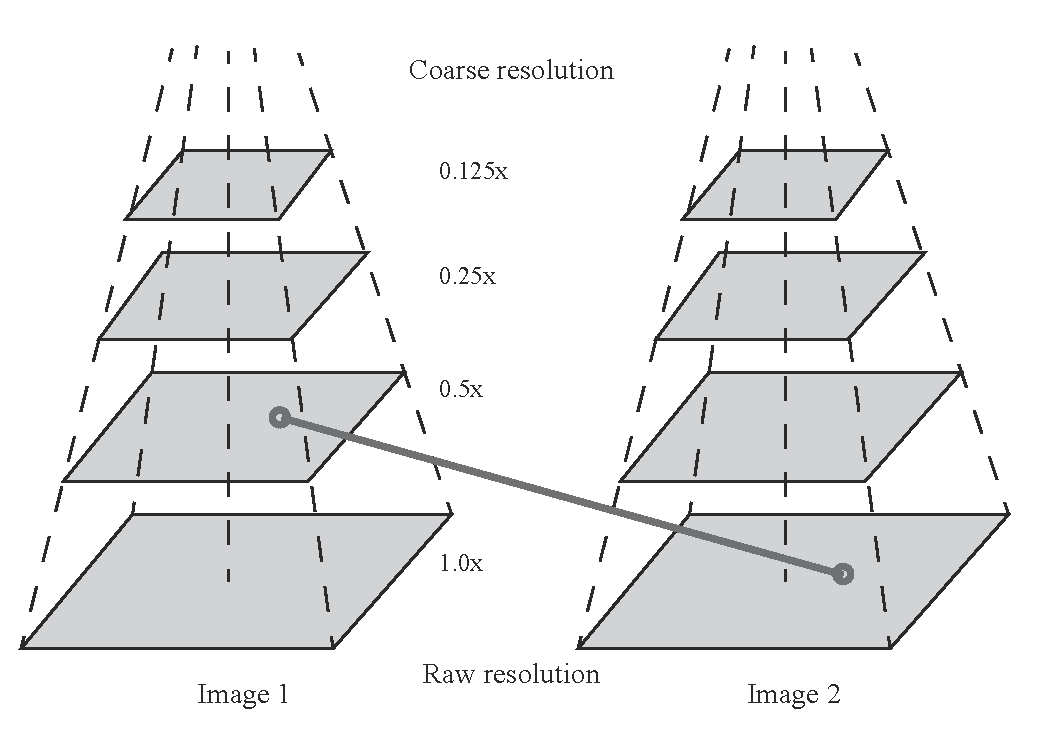
\includegraphics[width=0.9\linewidth]{vo1/pyramid}\\
    \caption{Use pyramids to match images at different resolutions.}
    \label{fig:pyramid}
\end{figure}

In terms of rotation, we calculate the gray centroid of the image near the feature point. The so-called centroid refers to the gray value of the image block as the center of weight. The specific steps are as follows {\cite{Rosin1999}}:

\begin{enumerate}
\item In a small image block $B$, define the moment of the image block as:
\[
m_{pq}=\sum_{x,y \in B}x^{p}y^{q}I(x,y), \quad p, q = \{0,1\}.
\]
\item Calculate the centroid of the image block by the moment:
\[
C=\left(\frac{m_{10}}{m_{00}},\frac{m_{01}}{m_{00}}\right).
\]
\item Connect the geometric center $O$ and the centroid $C$ of the image block to get a direction vector $\overrightarrow{OC}$, so the direction of the feature point can be defined as:
\[
\theta = \arctan(m_{01}/m_{10}).
\]
\end{enumerate}
FAST corner points have a description of scale and rotation, which significantly improves the robustness of their representation between different images. This improved FAST is called oriented FAST in ORB.

\subsubsection{BRIEF Descriptor}
After extracting the Oriented FAST key points, we calculate the descriptor for each point. ORB uses an improved BRIEF feature description. Let's first introduce what BRIEF is.

BRIEF is a binary descriptor. Its description vector consists of many zeros and ones, which encode the size relationship between two random pixels near the key point (such as $p$ and $q$): If $p$ is greater than $q$, then take 1, otherwise take 0. If we take 128 such $p,q$ pairs, we will finally get a 128-dimensional vector  {\cite{calonder2010brief}} consisting of 0s and 1s. The BRIEF implements the comparison of randomly selected points, which is very fast. Since it expresses in binary, it is also very convenient to store and suitable for real-time image matching. The original BRIEF descriptor does not have rotation invariance, so it is easy to get lost when the image is rotated. The ORB calculates the direction of the key points in the FAST feature point extraction stage. The direction information can be used to calculate the Steer BRIEF feature after the rotation so that the ORB descriptor has better rotation invariance.

Due to the consideration of rotation and scaling, the ORB performs well under translation, rotation, and scaling. Meanwhile, the combination of FAST and BRIEF is very efficient, which makes ORB features very popular in real-time SLAM. In \autoref{fig:ORB}~, we show the result of extracting ORB from an image. In the following, we will move on to feature matching between different images.

\begin{figure}[!htp]
    \centering
    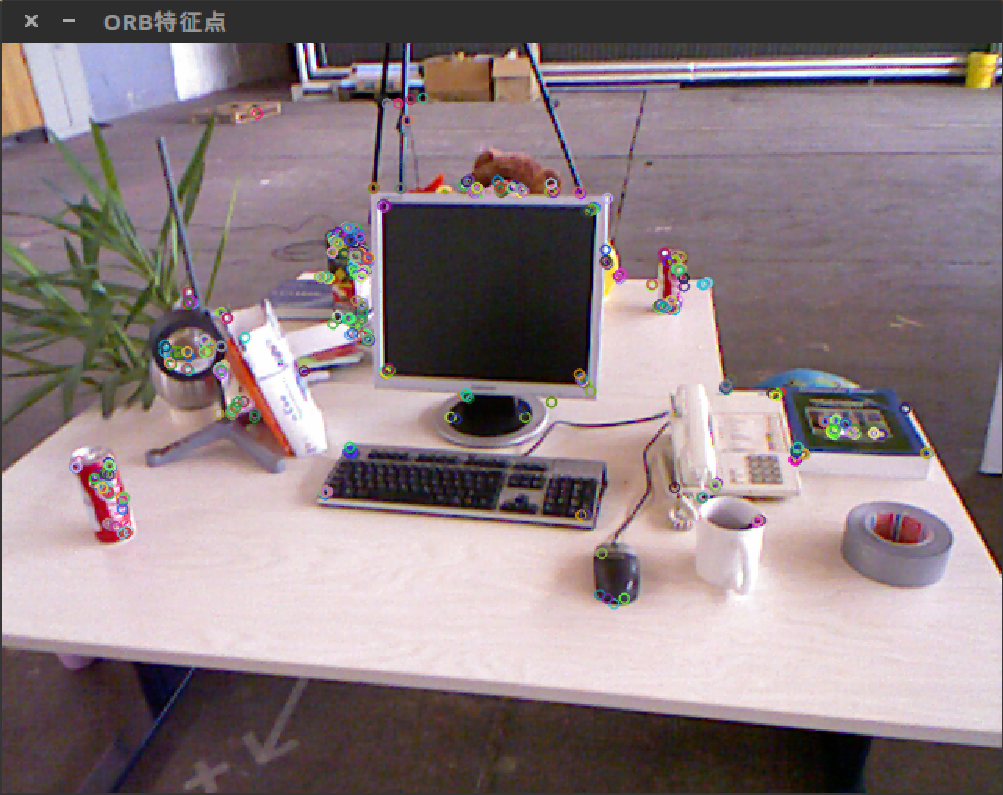
\includegraphics[width=0.9\linewidth]{vo1/feature}\\
    \caption{ORB feature points detected by OpenCV.}
    \label{fig:ORB}
\end{figure}

\subsection{Feature Matching}

Feature matching is a critical step in visual SLAM (\ref{fig:feature-matching}). Broadly speaking, feature matching solves the data association problem in SLAM, that is, to determine the view correspondence between the landmarks (feature points) and the landmarks (feature points) seen before. By accurately matching the descriptors between images or between images and maps, we can reduce a lot of work for subsequent pose estimation and optimization operations. However, due to the locality of image features, mismatches are common and have not been effectively resolved for a long time. It has become a significant bottleneck to improve the performance of visual SLAM. It is somehow due to repeated textures in the scene, making the feature descriptions very similar. Under this circumstance, it is hard to resolve the mismatch by using local features only.

\begin{figure}[!htp]
    \centering
    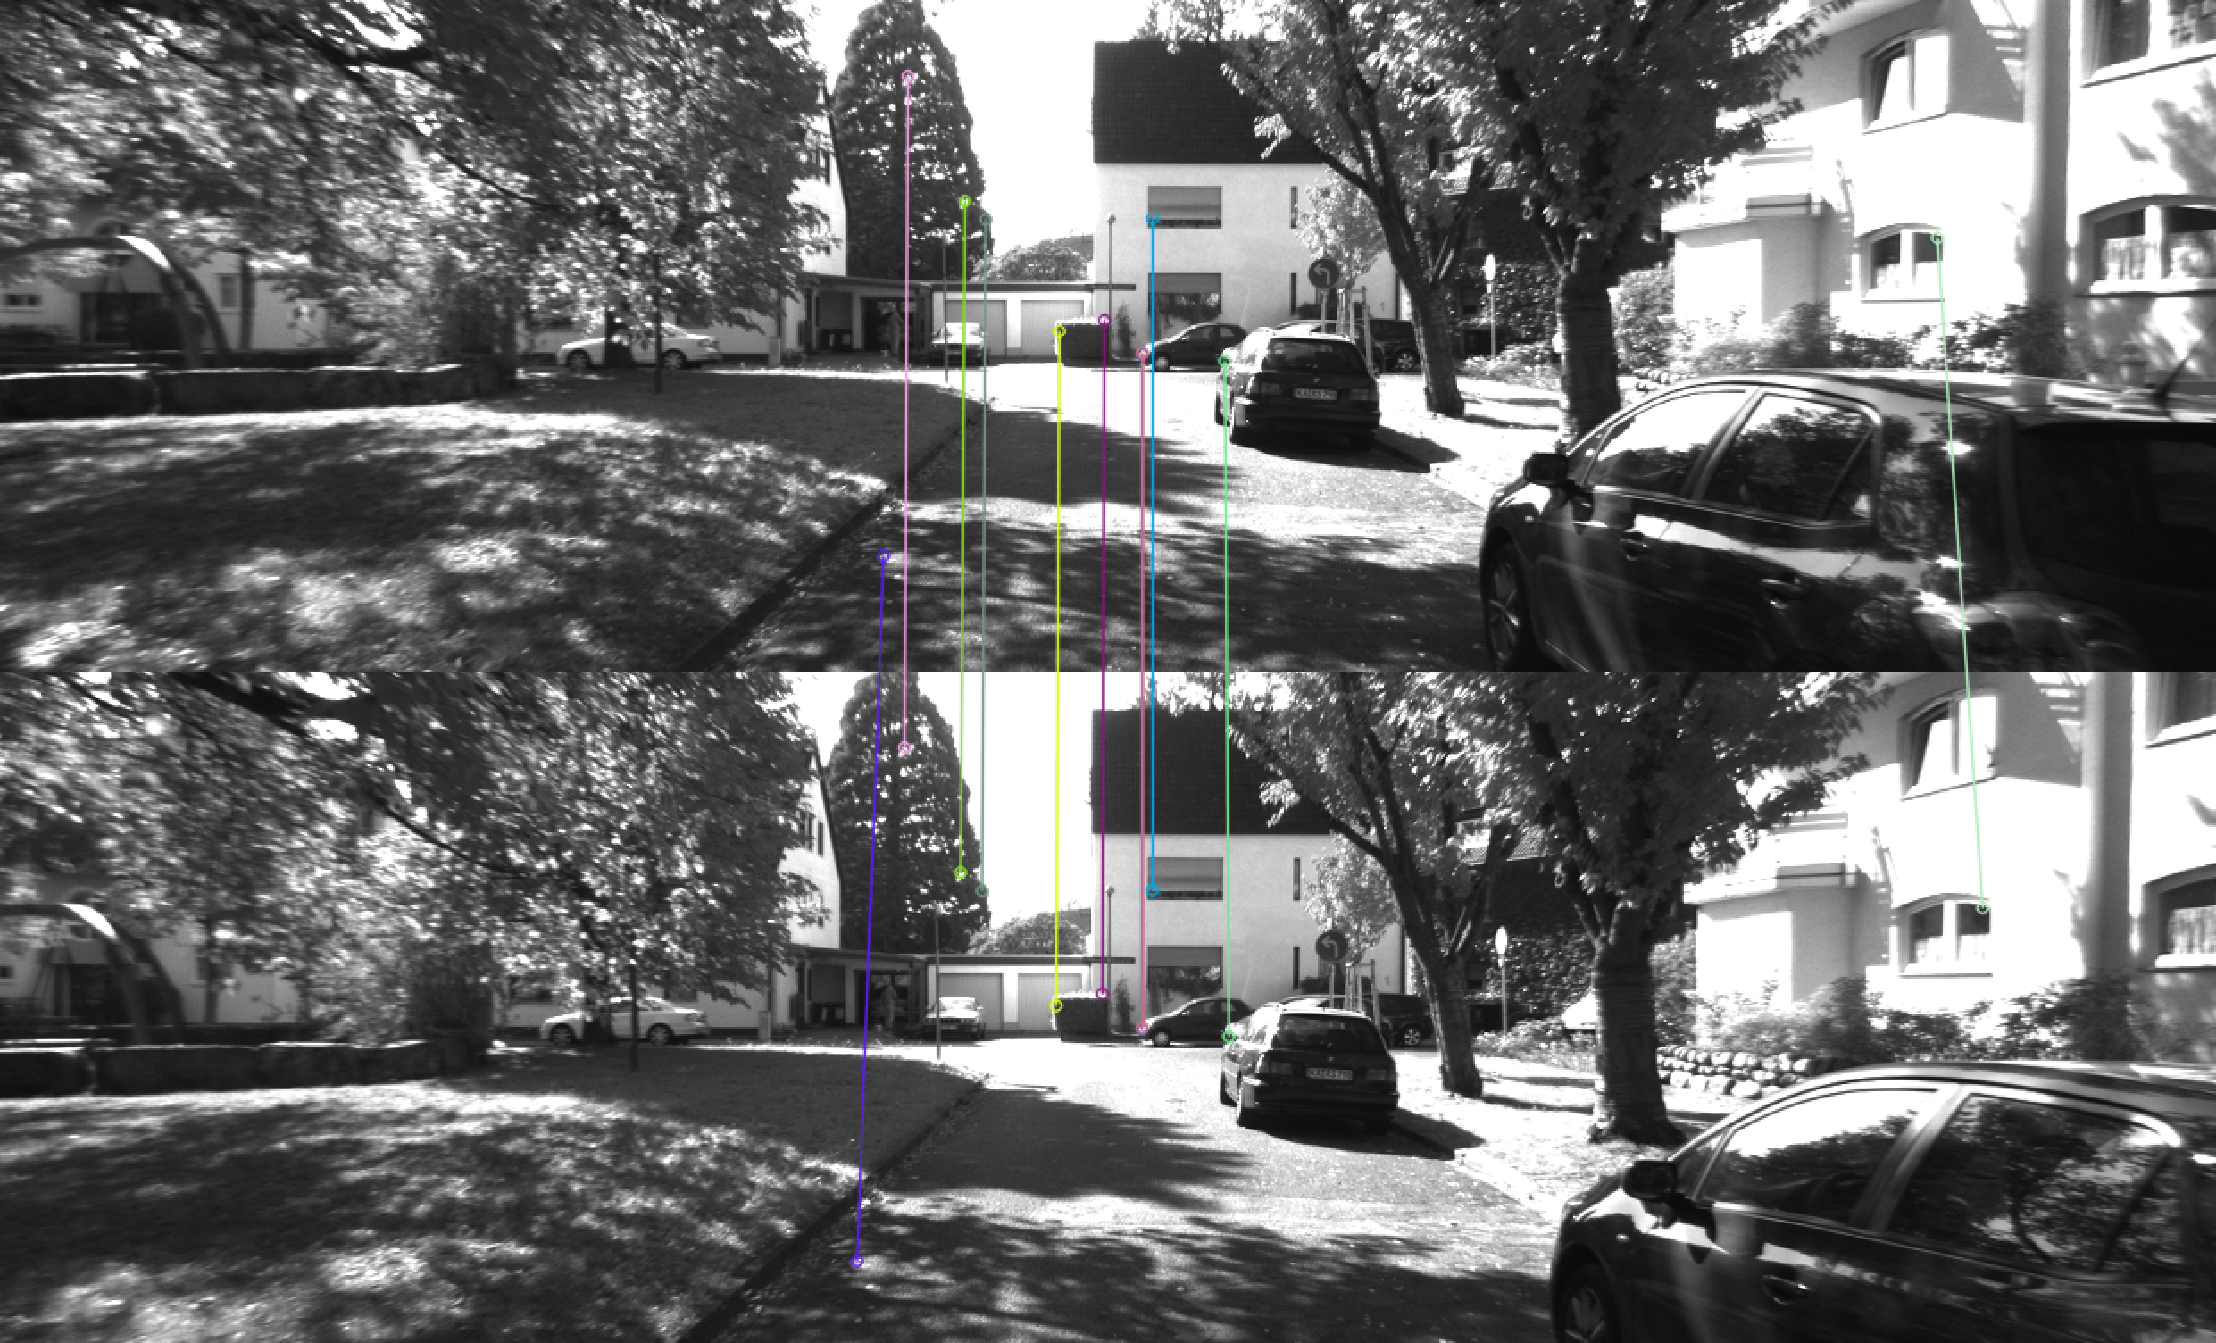
\includegraphics[width=0.9\linewidth]{vo1/feature-matching}
    \caption{Feature matching between two images.}
    \label{fig:feature-matching}
\end{figure}

However, let's first assume the matching is correct and then go back to discuss the mismatch problem. Consider images at two moments. Assume features $x_{t}^{m}, m=1,2,...,M$ are extracted in the image $I_{t}$, and $x_{t+1}^{n}, n=1,2,...,N$ in $I_{t+1}$ . How do we find the correspondence between these two sets? The simplest feature matching method is the brute-force matcher, which measures the distance between each pair of the features $x_{t}^{m}$ and all $x_{t+1}^{n}$ descriptors. Then sort the matching distance, and take the closest one as the matching point. The descriptor distance indicates the degree of similarity of two features. In practice, different distance metric norms can be used. For descriptors of floating-point type, using Euclidean distance to measure is a good choice. For binary descriptors (such as BRIEF), we often use Hamming distance as a metric. The Hamming distance between two binary vectors refers to the number of different digits.

When the number of feature points is large, the brute force matching's computational complexity will become too expensive, especially when you want to match a frame to a map. This does not meet our real-time requirements in SLAM. The Fast Approximate Nearest Neighbor (FLANN) algorithm is more suitable in this case. Since these matching algorithms' theory is mature and the implementation has already been integrated into OpenCV, the technical details will not be described here. Interested readers can refer to the literature \cite{Muja2009}.In engineering, we can also limit the search range of the brute-force method to achieve real-time performance.

\section{Practice: Feature Extraction and Matching}
\begin{figure}[!htp]
	\centering
	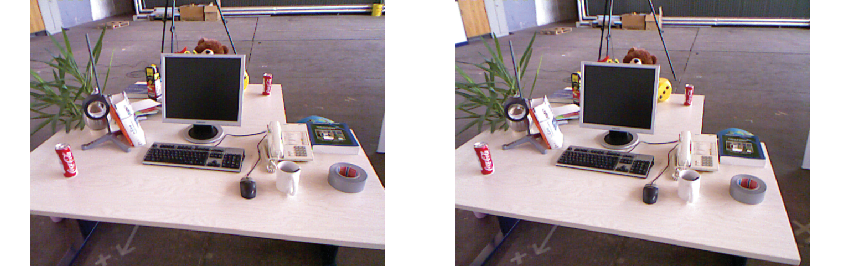
\includegraphics[width=0.9\linewidth]{vo1/exp1-images.pdf}
	\caption{Two images used in the practice.}
	\label{fig:exp1-images}
\end{figure}

OpenCV has integrated most of the image features, and we can easily use them by function calls. Let's demonstrate two examples here. In the first one, we show the use of OpenCV for feature matching of ORB; in the second, we explain how to write an ORB feature from scratch based on the principles. Through the practice, readers will have a deeper understanding of the ORB calculation process. Then other features can be done analogously.

\subsection{ORB Features in OpenCV}
First, we call OpenCV to extract and match ORB. We prepared two images for this practice, 1.png and 2.png under \textit{slambook2/ch7/}, as shown in \autoref{fig:exp1-images}~. They are two images from the public dataset \cite{Sturm2012}. We can see a slight movement of the camera. The procedure in this section demonstrates how to extract ORB features and perform matching. In the next section, we will show how to use matching results to estimate camera motion.

The following program demonstrates how to use ORB:
\begin{lstlisting}[language=c++,caption=slambook2/ch7/orb_cv.cpp]
#include <iostream>
#include <opencv2/core/core.hpp>
#include <opencv2/features2d/features2d.hpp>
#include <opencv2/highgui/highgui.hpp>
#include <chrono>

using namespace std;
using namespace cv;

int main(int argc, char **argv) {
	if (argc != 3) {
		cout << "usage: feature_extraction img1 img2" << endl;
		return 1;
	}
	//-- read images
	Mat img_1 = imread(argv[1], CV_LOAD_IMAGE_COLOR);
	Mat img_2 = imread(argv[2], CV_LOAD_IMAGE_COLOR);
	assert(img_1.data != nullptr && img_2.data != nullptr);
	
	//-- initialization
	std::vector<KeyPoint> keypoints_1, keypoints_2;
	Mat descriptors_1, descriptors_2;
	Ptr<FeatureDetector> detector = ORB::create();
	Ptr<DescriptorExtractor> descriptor = ORB::create();
	Ptr<DescriptorMatcher> matcher = DescriptorMatcher::create("BruteForce-Hamming");
	
	//-- detect  Oriented FAST
	chrono::steady_clock::time_point t1 = chrono::steady_clock::now();
	detector->detect(img_1, keypoints_1);
	detector->detect(img_2, keypoints_2);
	
	//-- compute BRIEF descriptor
	descriptor->compute(img_1, keypoints_1, descriptors_1);
	descriptor->compute(img_2, keypoints_2, descriptors_2);
	chrono::steady_clock::time_point t2 = chrono::steady_clock::now();
	chrono::duration<double> time_used = chrono::duration_cast<chrono::duration<double>>(t2 - t1);
	cout << "extract ORB cost = " << time_used.count() << " seconds. " << endl;
	
	Mat outimg1;
	drawKeypoints(img_1, keypoints_1, outimg1, Scalar::all(-1), DrawMatchesFlags::DEFAULT);
	imshow("ORB features", outimg1);
	
	//-- use Hamming distance to match the features
	vector<DMatch> matches;
	t1 = chrono::steady_clock::now();
	matcher->match(descriptors_1, descriptors_2, matches);
	t2 = chrono::steady_clock::now();
	time_used = chrono::duration_cast<chrono::duration<double>>(t2 - t1);
	cout << "match ORB cost = " << time_used.count() << " seconds. " << endl;
	
	//-- sort and remove the outliers
	// min and max distance
	auto min_max = minmax_element(matches.begin(), matches.end(),
		[](const DMatch &m1, const DMatch &m2) { return m1.distance < m2.distance; });
	double min_dist = min_max.first->distance;
	double max_dist = min_max.second->distance;
	
	printf("-- Max dist : %f \n", max_dist);
	printf("-- Min dist : %f \n", min_dist);
	
	// remove the bad matching
	std::vector<DMatch> good_matches;
	for (int i = 0; i < descriptors_1.rows; i++) {
		if (matches[i].distance <= max(2 * min_dist, 30.0)) {
			good_matches.push_back(matches[i]);
		}
	}
	
	//-- draw the results
	Mat img_match;
	Mat img_goodmatch;
	drawMatches(img_1, keypoints_1, img_2, keypoints_2, matches, img_match);
	drawMatches(img_1, keypoints_1, img_2, keypoints_2, good_matches, img_goodmatch);
	imshow("all matches", img_match);
	imshow("good matches", img_goodmatch);
	waitKey(0);
	
	return 0;
}
\end{lstlisting}

Run this program (you need to enter the paths of two images manually). The screen output should be like this:
\begin{lstlisting}[language=sh,caption=Terminal input:]
% build/orb_cv 1.png 2.png
extract ORB cost = 0.0229183 seconds. 
match ORB cost = 0.000751868 seconds.
-- Max dist : 95.000000 
-- Min dist : 4.000000 
\end{lstlisting}

\autoref{fig:exp1-results}~shows the results of the example. We see a large number of false matches before the filtering. After removing the bad matches, most of the remaining matches are correct. Here, we followed an empirical rule in engineering that good matches are selected from where the Hamming distance is less than twice the minimum distance. It may not have a theoretical explanation but just an engineering trick. However, although we can select out the correct matches in the example image, we still cannot guarantee that the remaining matches are correct. Therefore, during the motion estimation step, it is necessary to consider those mismatches. ORB extraction took 22.9 milliseconds (two images) on my machine, and matching took 0.75 milliseconds. It can be seen that most of the calculation is spent on feature extraction.

\begin{figure}[!htp]
	\centering
	\includegraphics[width=1.0\linewidth]{vo1/exp1-result}
	\caption{Feature extraction and matching results.}
	\label{fig:exp1-results} 
\end{figure}

\subsection{ORB Features from Scratch}
Below we show the method of coding ORB features from scratch. Since the code is a bit long, only a snippet is shown here. Readers are recommended to obtain the rest from the GitHub codebase.
\begin{lstlisting}[language=c++,caption=slambook2/ch7/orb_self.cpp (part)]
typedef vector<uint32_t> DescType;
// ... omit some image loading and testing code
// compute the descriptor
void ComputeORB(const cv::Mat &img, vector<cv::key point> &key points, vector<DescType> &descriptors) {
    const int half_patch_size = 8;
    const int half_boundary = 16;
    int bad_points = 0;
    for (auto &kp: key points) {
        if (kp.pt.x < half_boundary || kp.pt.y < half_boundary ||
        kp.pt.x >= img.cols - half_boundary || kp.pt.y >= img.rows - half_boundary) {
            // outside
            bad_points++;
            descriptors.push_back({});
            continue;
        }
    
        float m01 = 0, m10 = 0;
        for (int dx = -half_patch_size; dx < half_patch_size; ++dx) {
            for (int dy = -half_patch_size; dy < half_patch_size; ++dy) {
                uchar pixel = img.at<uchar>(kp.pt.y + dy, kp.pt.x + dx);
                m01 += dx * pixel;
                m10 += dy * pixel;
            }
        }
    
        // angle should be arc tan(m01/m10);
        float m_sqrt = sqrt(m01 * m01 + m10 * m10);
        float sin_theta = m01 / m_sqrt;
        float cos_theta = m10 / m_sqrt;
        
        // compute the angle of this point
        DescType desc(8, 0);
        for (int i = 0; i < 8; i++) {
            uint32_t d = 0;
            for (int k = 0; k < 32; k++) {
                int idx_pq = i * 8 + k;
                cv::Point2f p(ORB_pattern[idx_pq * 4], ORB_pattern[idx_pq * 4 + 1]);
                cv::Point2f q(ORB_pattern[idx_pq * 4 + 2], ORB_pattern[idx_pq * 4 + 3]);
        
                // rotate with theta
                cv::Point2f pp = cv::Point2f(cos_theta * p.x - sin_theta * p.y, sin_theta * p.x + cos_theta * p.y) + kp.pt;
                cv::Point2f qq = cv::Point2f(cos_theta * q.x - sin_theta * q.y, sin_theta * q.x + cos_theta * q.y) + kp.pt;	
                
                // compare pp and qq
                if (img.at<uchar>(pp.y, pp.x) < img.at<uchar>(qq.y, qq.x)) {
                    d |= 1 << k;
                }
            }
            desc[i] = d;
        }
        descriptors.push_back(desc);
    }
    
    cout << "bad/total: " << bad_points << "/" << key points.size() << endl;
}

// brute-force matching
void BfMatch(
    const vector<DescType> &desc1, const vector<DescType> &desc2, vector<cv::DMatch> &matches) {
    const int d_max = 40;
    
    for (size_t i1 = 0; i1 < desc1.size(); ++i1) {
        if (desc1[i1].empty()) continue;
        cv::DMatch m{i1, 0, 256};
        for (size_t i2 = 0; i2 < desc2.size(); ++i2) {
            if (desc2[i2].empty()) continue;
            int distance = 0;
            for (int k = 0; k < 8; k++) {
                distance += _mm_popcnt_u32(desc1[i1][k] ^desc2[i2][k]);
            }
            if (distance < d_max && distance < m.distance) {
                m.distance = distance;
                m.trainIdx = i2;
            }
        }
        if (m.distance < d_max) {
            matches.push_back(m);
        }
    }
}
\end{lstlisting}
We only show the ORB calculation and matching code. In the calculation, we use 256-bit binary description, which corresponds to 8 32-bit unsigned int data expressed as DescType with typedef. Then, we calculate the FAST feature point's angle according to the principle introduced above and then use the angle to calculate the descriptor. To accelerate, some complicated calculations, such as $\arctan$, $\sin$, and $\cos$, are worked around by the principle of trigonometric functions. In the BfMatch function, we also use the \_mm\_popcnt\_u32 function in the SSE instruction set to calculate the number of 1s in an unsigned int, which is used to achieve the effect of calculating the Hamming distance. The result of this program is as follows, and the matching result is shown in \autoref{fig:matches}:

\begin{lstlisting}[language=sh,caption=Terminal output:]
bad/total: 43/638
bad/total: 8/595
extract ORB cost = 0.00390721 seconds.
match ORB cost = 0.000862984 seconds.
matches: 51
\end{lstlisting}

\begin{figure}[!htp]
    \centering
    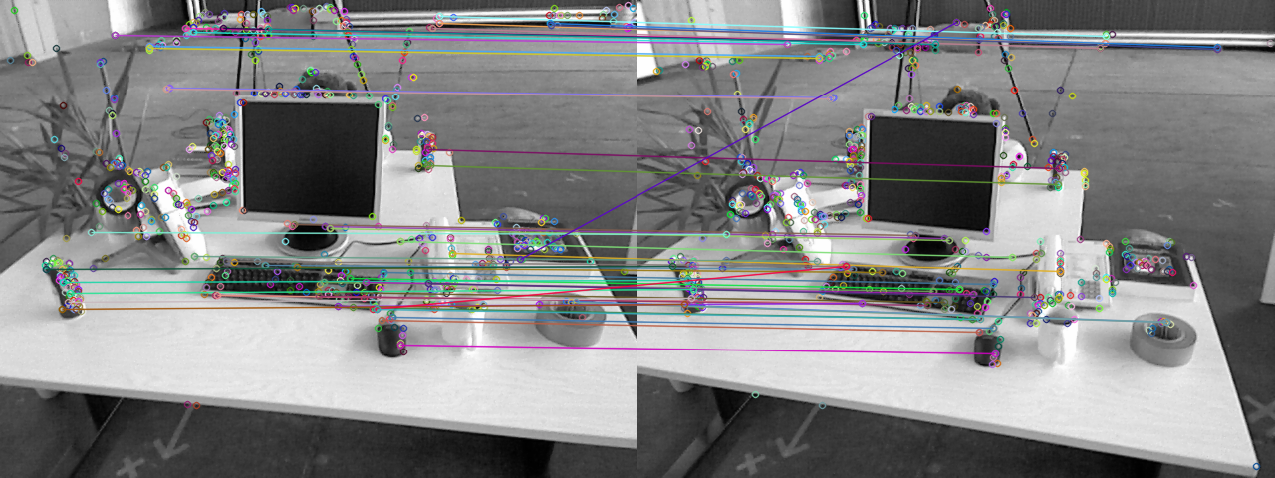
\includegraphics[width=0.8\linewidth]{vo1/matches}
    \caption{Matching Result}
    \label{fig:matches}
\end{figure}

In this program, ORB extraction takes 3.9 milliseconds, and the matching takes only 0.86 milliseconds. Through some simple modifications in implementation, we accelerated the extraction of ORB by 5.8 times. Note that compiling this program requires your CPU to support the SSE instruction set, which should be already supported on most modern PC CPUs. If we can further parallelize the feature extraction, the algorithm can be further accelerated.

\subsection{Calculate the Camera Motion}
Now, we have key points matching. In the next step, we need to estimate the camera's motion based on the matching. It is totally different for different camera settings (or the information available for the calculation):

\begin{enumerate}
	\item When the camera is monocular, we only know the 2D pixel coordinates, so the problem is to estimate the motion according to two sets of 2D points. This problem is solved by \textit{epipolar geometry}.
	\item When the camera is binocular, RGB-D, or the distance is obtained by some method, then the problem is to estimate the motion according to two sets of 3D points. This problem is usually solved by ICP.
	\item If one set is 3D and one set is 2D, we get some 3D points and their projection positions on the camera, and we can also estimate the camera's pose. This problem is solved by \textit{PnP}.
\end{enumerate}

The following sections will introduce camera motion estimation in these three situations. We will start from the 2D-2D case with the least information and see how it is dealt with and troublesome problems.

\section{2D−2D: Epipolar Geometry}
\label{sec:epipolar-geometry}

\subsection{Epipolar Constraints}

Suppose we have a pair of matched feature points from two images, as shown in \autoref{fig:doubleview}~. If there are several pairs of such matching points, the camera motion between the two frames can be recovered through the correspondence between these two-dimensional image points. How many pairs do we need? We will see later. Let's first take a look at the geometric relationship between the matching points in the two images.

\begin{figure}[!htp]
	\centering
	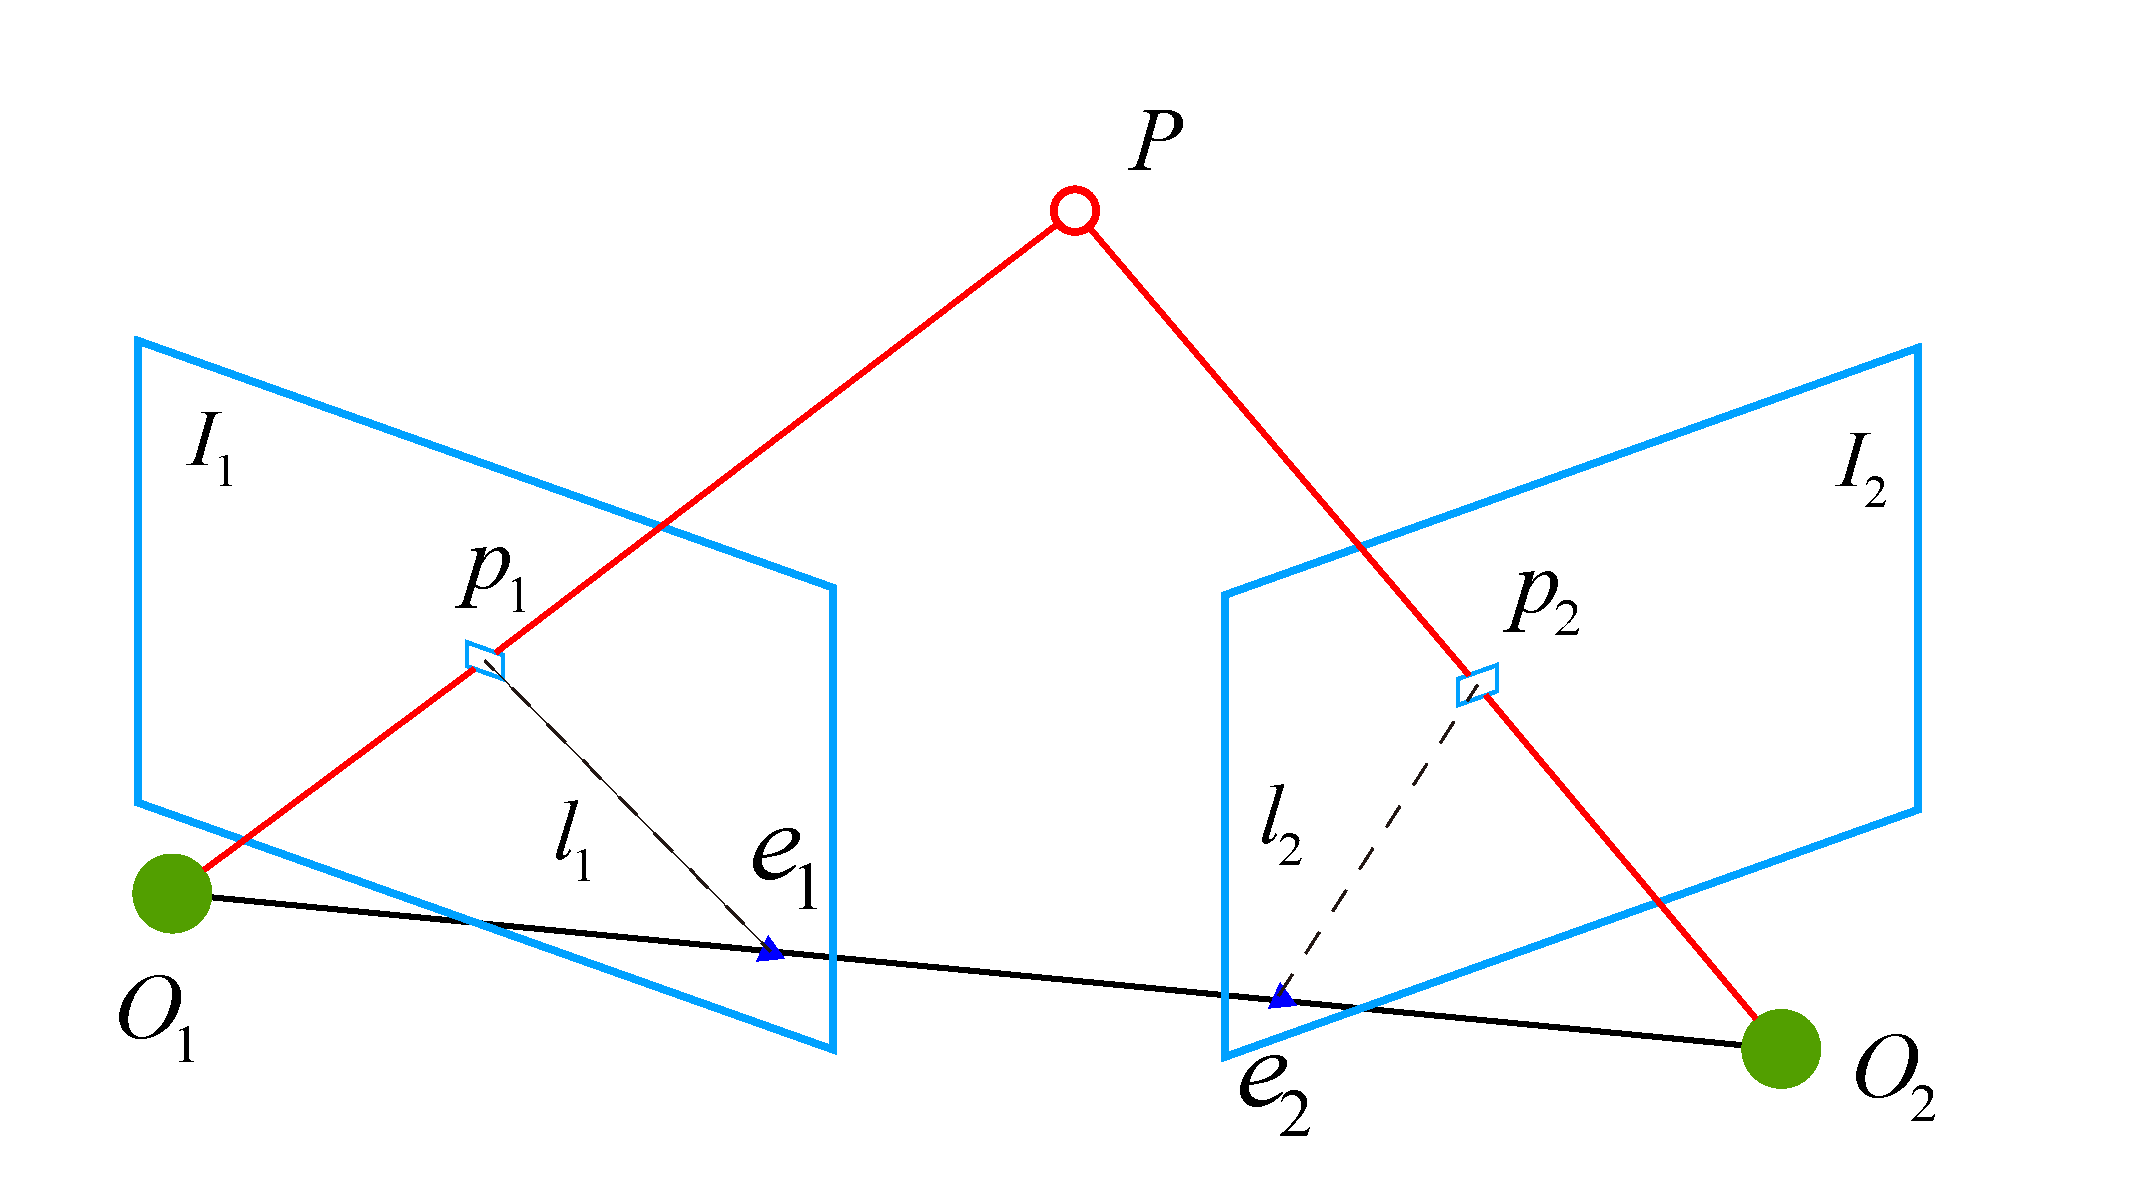
\includegraphics[width=0.6\linewidth]{vo1/fundamental}
	\caption{The epipolar constraints.}
	\label{fig:doubleview}
\end{figure}

Take \autoref{fig:doubleview}~ as an example. Our goal is to find the motion between two frames $I_{1}, I_{2}$. Define the motion from the first frame to the second frame as $\mathbf{R}, \mathbf{t}$, and the centers of the two cameras as $O_{1}, O_{2}$. Now, consider that there is a feature point $p_{1}$ in $I_{1}$, which corresponds to the feature point $p_{2}$ in $I_{2}$, obtained through feature matching. If the matching is correct, it means that they are indeed the projection of the same point. Now we need some terms to describe the geometric relationship between them. First, the line $\overrightarrow{O_{1}p_{1}}$ and the line $\overrightarrow{O_{2}p_{2}}$ will intersect at the point $P$ in the 3D space. The three points $O_{1}, O_{2}, and P$ can determine a plane, and it is called the epipolar plane. The intersection of the line of $O_{1}O_{2}$ and the image plane $I_{1}, I_{2}$ is $e_{1}, e_{2}$, respectively. The $e_{1}, e_{2}$ is called epipoles, and $O_{1}O_{2}$ is called the baseline. We call the intersecting line $l_{1},l_{2}$ between the polar plane and the two image planes $I_{1}, I_{2}$ as the epipolar line.

From the first frame, the ray $\overrightarrow{O_1 p_1}$ represents the possible spatial locations where a pixel may appear since all points on the ray will be projected to the same pixel. Meanwhile, suppose we don't know the location of $P$. When we look at the second image, the connection $\overrightarrow{e_2 p_2}$ (i.e., the epipolar line in the second image) is the possible projected positions of the point $P$, as well as the projection of the ray $\overrightarrow{O_1 p_1}$ in the second image. Now, since we have determined the pixel location of $p_2$ through feature matching, we can infer the spatial location of $P$ and the camera movement, as long as the feature matching is correct. If there is no feature matching, we can't determine where the $p_2$ is on the epipolar line. At that time, we must search on the epipolar line $l_2$ to get the correct match, which will be discussed in lecture \ref{cpt:12}.

Now, let's look at the geometric relationship algebraically. Define the spatial position of $P$ in the first frame to be:
\[
\mathbf{P}=[X,Y,Z]^T.
\]
According to the pinhole camera model introduced in lecture \ref{cpt:5}, we know that the pixel positions of the two pixels $\mathbf{p}_1,\mathbf{p}_2$ are:
\begin{equation}
\label{eq:7.1}
s_1 {\mathbf{p}_1} = \mathbf{KP},\quad s_2 \mathbf{p}_2 = \mathbf{K}\left( \mathbf{RP + t} \right),
\end{equation}
where $\mathbf{K}$ is the camera intrinsic  matrix, and $\mathbf{R}, \mathbf{t}$ are the camera motions between two frames. Specifically, they are $\mathbf{R}_{21}$ and $\mathbf{t}_{21}$, i.e. transformation from the first frame to the second. We can also write them in Lie algebra form.

Sometimes, we use homogeneous coordinates to represent pixels. When using homogeneous coordinates, a vector will be equal to itself multiplied by any non-zero constant. This is usually used to express a projection relationship. For example, $s_1 \mathbf{p}_1$ and $\mathbf{p}_1$ form a projection relationship, and they are equal in the sense of homogeneous coordinates. We call this equal \textit{up to a scale}, denoted as:
\begin{equation}
s\mathbf{p} \simeq \mathbf{p}.
\end{equation}
Then, the relationship between two projections can be written as:
\begin{equation}
 {\mathbf{p}_1} \simeq \mathbf{KP},\quad \mathbf{p}_2 \simeq \mathbf{K}\left( \mathbf{RP + t} \right).
\end{equation}

Now, let
\begin{equation}
{\mathbf{x}_1} = {\mathbf{K}^{ - 1}}{\mathbf{p}_1}, \quad {\mathbf{x}_2} = {\mathbf{K}^{ - 1}}{\mathbf{p}_2}.
\end{equation}

Here, $\mathbf{x}_1, \mathbf{x}_2$ are the coordinates on the normalized plane of two pixels. Substituting to the above equation, we get:
\begin{equation}
{\mathbf{x}_2} \simeq \mathbf{R} {\mathbf{x}_1} + \mathbf{t}.
\end{equation}

Left multiply both sides by $\mathbf{t}^\wedge$. Recalling the definition of $^\wedge$, this is equivalent to the outer product of both sides with $\mathbf{t}$:
\begin{equation}
\mathbf{t}^\wedge \mathbf{x}_2 \simeq \mathbf{t}^\wedge \mathbf{R} \mathbf{x}_1.
\end{equation}

Then, left multiply $\mathbf{x}_2^T$ on both sides:
\begin{equation}
\mathbf{x}_2^T \mathbf{t}^\wedge \mathbf{x}_2 \simeq \mathbf{x}_2^T \mathbf{t}^\wedge \mathbf{R} \mathbf{x}_1.
\end{equation}

On the left side, $\mathbf{t}^\wedge \mathbf{x}_2$ is a vector orthogonal to both $\mathbf{t}$ and $\mathbf{x}_2$. So its inner product with $\mathbf{x}_2$ will get 0. Since the left side of the equation is strictly zero, it is also zero after multiplying by any non-zero constant, so we can turn $\simeq$ back to the usual equal sign. Therefore, we have a concise equation:
\begin{equation}
\mathbf{x}_2^T \mathbf{t}^\wedge \mathbf{R} \mathbf{x}_1 = 0.
\end{equation}

Substituting the $\mathbf{p}_1, \mathbf{p}_2$ again, we have:
\begin{equation}
\mathbf{p}_2^T \mathbf{K}^{-\mathrm{T}} \mathbf{t}^\wedge \mathbf{R} \mathbf{K}^{-1} \mathbf{p}_1  = 0.
\end{equation}

Both equations are called \textbf{epipolar constraint}, which is famous for its conciseness. Geometrically, it means $O_1, P, O_2$ are coplanar. The epipolar constraint encodes both translation and rotation. We define two matrices: \textit{Fundamental} matrix $\mathbf{F}$ and \textit{essential} Matrix $\mathbf{E}$ from this equation: 
\begin{equation}
\mathbf{E} = \mathbf{t}^ \wedge \mathbf{R}, \quad \mathbf{F} = \mathbf{K}^{ -\mathrm{T}} \mathbf{E} {\mathbf{K}^{ - 1}}, \quad \mathbf{x}_2^T \mathbf{E} {\mathbf{x}_1} = \mathbf{p}_2^T \mathbf{F} {\mathbf{p}_1} = 0.
\end{equation}

The epipolar constraint gives the spatial relationship of two matching points concisely. Therefore, the camera pose estimation problem can be summarized as the following two steps:

\begin{enumerate}
	\item Find $\mathbf{E}$ or $\mathbf{F}$ based on the pixel positions of the matched points.
	\item Find $\mathbf{R}, \mathbf{t}$ based on $\mathbf{E}$ or $\mathbf{F}$.
\end{enumerate}

Since $\mathbf{E}$ and $\mathbf{F}$ only differ from the camera internal parameters, and the internal parameters are assumed to be known in SLAM problem \footnote{However, in SfM research, it may be unknown and need to be estimated. }, so the simpler form $\mathbf{E}$ is often used in practice. Let's take $\mathbf{E}$ as an example to introduce how to solve the above two problems.

\subsection{Essential Matrix}
By definition, the essential matrix $\mathbf{E} = \mathbf{t}^\wedge \mathbf{R}$. It is a matrix of $3\times 3$ with 9 unknown variables. So, can any matrix of the size $3 \times 3$ be an essential matrix? From the structure of $\mathbf{E}$, there are the following points worth noting:

\begin{itemize}
	\item The essential matrix is defined by the epipolar constraint. Since the epipolar constraint is the constraint of an\textit{ equal-to-zero }equation, after multiplying $\mathbf{E}$ by any non-zero constant, the constraint is still satisfied. We call this $\mathbf{E}$ 's equivalence under different scales.
	\item According to $\mathbf{E} = \mathbf{t}^ \wedge \mathbf{R}$, it can be proved that  {\cite{Hartley2003}}, the singular value of the essential matrix $\mathbf{E}$ must be in the form of $[\sigma, \sigma, 0]^T$. This is called internal properties of essential matrix.
	\item On the other hand, since translation and rotation each have 3 degrees of freedom, $\mathbf{t}^\wedge \mathbf{R}$ has 6 degrees of freedom. But due to the equivalence of scales, $\mathbf{E}$ actually has 5 degrees of freedom.
\end{itemize}

The fact that $\mathbf{E}$ has 5 degrees of freedom indicates that we can use at least 5 pairs of points to solve $\mathbf{E}$. However, the internal property of $\mathbf{E}$ is nonlinear, which could cause trouble in the estimation. Therefore, it is also possible to consider only its scale equivalence and use 8 pairs of matched points to estimate $\mathbf{E}$. This is the classic \textit{eight-point-algorithm} {\cite{Hartley1997, Longuet-Higgins1987}}. The eight-point method only uses the linear properties of $\mathbf{E}$, so it can be solved under the framework of linear algebra. Let's take a look at how the eight-point method works.

Consider a pair of matched points, their normalized coordinates are $\mathbf{x}_{1}=[u_{1},v_{1},1]^T$, $\mathbf{x}_{2}=[u_{2},v_{2},1]^T$. According to the polar constraints, we have:
\begin{equation}
\begin{pmatrix} 
u_{2},v_{2},1
\end{pmatrix}
\begin{pmatrix}
 e_{1} & e_{2} & e_{3}\\ 
 e_{4} & e_{5} & e_{6}\\ 
 e_{7} & e_{8} & e_{9} 
\end{pmatrix}
\begin{pmatrix} 
u_{1}\\v_{1}\\1
\end{pmatrix}
=0.
\end{equation}

We rewrite the matrix $\mathbf{E}$ in the vector form:
\[
\mathbf{e}= [e_{1},e_{2},e_{3},e_{4},e_{5},e_{6},e_{7},e_{8},e_{9}]^T,
\]
Then the epipolar constraint can be written in a linear form related to $\mathbf{e}$:
\begin{equation}
[u_{2}u_{1},u_{2}v_{1},u_{2},v_{2}u_{1},v_{2}v_{1},v_{2},u_{1},v_{1},1] \cdot  \mathbf{e}=0.
\end{equation}

Analogously, we stack all the points into one equation and obtain a linear equation system (where $u^i, v^i$ represent the $i$-th feature point): 
\begin{equation}
\label{Eq:eight-point}
\begin{pmatrix}
u_{2}^{1}u_{1}^{1}& u_{2}^{1}v_{1}^{1}& u_{2}^{1}& v_{2}^{1}u_{1}^{1}& v_{2}^{1}v_{1}^{1}& v_{2}^{1} &u_{1}^{1} &v_{1}^{1}&1\\
u_{2}^{2}u_{1}^{2}& u_{2}^{2}v_{1}^{2}& u_{2}^{2}& v_{2}^{2}u_{1}^{2}& v_{2}^{2}v_{1}^{2}& v_{2}^{2} &u_{1}^{2} &v_{1}^{2}&1\\
\vdots & \vdots & \vdots & \vdots & \vdots & \vdots & \vdots & \vdots \\
u_{2}^{8}u_{1}^{8}& u_{2}^{8}v_{1}^{8}& u_{2}^{8}& v_{2}^{8}u_{1}^{8}& v_{2}^{8}v_{1}^{8}& v_{2}^{8} &u_{1}^{8}&v_{1}^{8}&1\\
\end{pmatrix}
\begin{pmatrix}
e_{1}\\ e_{2}\\ e_{3}\\  e_{4}\\ e_{5}\\ e_{6}\\ e_{7}\\ e_{8}\\ e_{9}  
\end{pmatrix}
=0.
\end{equation}


These eight equations form a linear equation system. Its coefficient matrix is composed of 2D feature point positions, and its size is $8 \times 9$. $\mathbf{e}$ is located in the null space of this matrix. If the coefficient matrix is of full rank (i.e., 8), then its null space dimension is 1, meaning that $\mathbf{e}$ forms a line. This is consistent with the scale equivalence of $\mathbf{e}$. If the matrix composed of 8 pairs of matching points meets the condition of rank 8, then the elements of $\mathbf{E}$ can be solved uniquely by the above equation.

The next question is how to recover the movement of the camera $\mathbf{R}, \mathbf{t}$ according to the estimated essential matrix $\mathbf{E}$. This process is obtained by singular value decomposition (SVD). Let the SVD decomposition of $\mathbf{E}$ be:
\begin{equation}
\mathbf{E} = \mathbf{U} \boldsymbol{\Sigma} \mathbf{V}^T,
\end{equation}
where $\mathbf{U}, \mathbf{V}$ are orthogonal matrices, and $\boldsymbol{\Sigma}$ is the  singular value matrice. According to the internal properties of $\mathbf{E}$, we know that $\boldsymbol{\Sigma} = \mathrm{diag}( \sigma, \sigma, 0 )$. In SVD decomposition, for any $\mathbf{E}$, there are two possible $\mathbf{t}, \mathbf{R}$:
\begin{equation}
\begin{array}{l}
\mathbf{t}_1^ \wedge  = \mathbf{U}{\mathbf{R}_Z}(\frac{\pi }{2}) \boldsymbol{\Sigma} {\mathbf{U}^T}, \quad {\mathbf{R}_1} = \mathbf{U} \mathbf{R}_Z^T(\frac{\pi }{2}){ \mathbf{V}^T}\\
\mathbf{t}_2^ \wedge  = \mathbf{U}{\mathbf{R}_Z}( - \frac{\pi }{2})\boldsymbol{\Sigma} {\mathbf{U}^T}, \quad  {\mathbf{R}_2} = \mathbf{U} \mathbf{R}_Z^T( - \frac{\pi }{2}){\mathbf{V}^T}.
\end{array}
\end{equation}

Among them, $\mathbf{R}_Z\left(\frac{\pi }{2}\right)$ represents the rotation matrix obtained by rotating $90^\circ$ along the $Z$ axis. Since $-\mathbf{E}$ is equivalent to $\mathbf{E}$, taking the minus sign for any $\mathbf{t}$ will also get the same result. Therefore, when decomposing from $\mathbf{E}$ to $\mathbf{t}, \mathbf{R}$, there are a total of \textbf{four} possible solutions.

\autoref{fig:epipolar-solution}~ shows the four solutions obtained by decomposing the essential matrix. We know the projection (red) of the space point on the camera (blue line) and want to solve the camera's motion. In the case of keeping the redpoint unchanged, four possible situations can be drawn. Fortunately, only in the first solution, $P$ has positive depths in both cameras. Therefore, we can substitute any points into the four solutions and check the depth's sign to determine which solution is correct.

\begin{figure}[!htp]
	\centering
	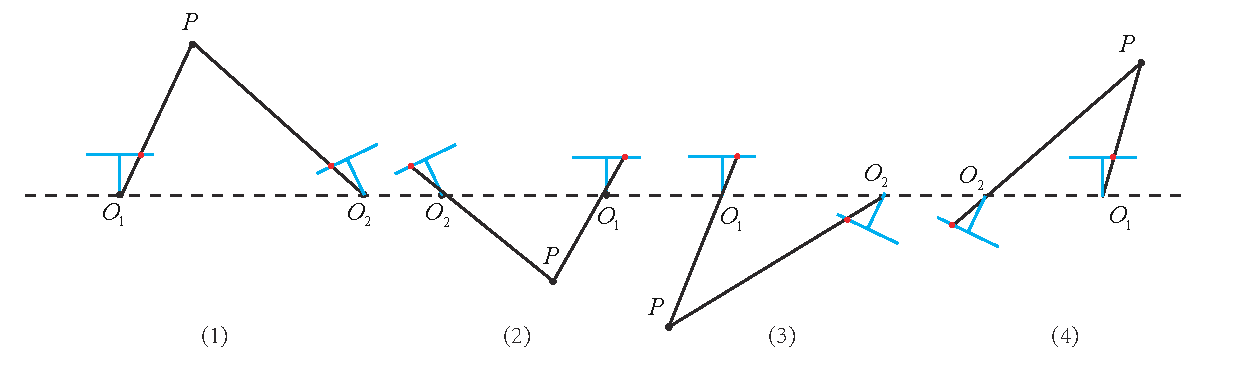
\includegraphics[width=1.0\linewidth]{vo1/epipolar-solution}
	\caption{We get four solutions when decomposing the essential matrix. }
	\label{fig:epipolar-solution}
\end{figure}

If we use the internal properties of $\mathbf{E}$, then it has only five degrees of freedom. So at least five pairs of matched points can be used to solve the camera motion {\cite{Li2006, Nister2004a}}. However, this approach is more complicated. Since there are usually dozens or even hundreds of matching points for engineering realization, it is often not helpful to reduce from 8 pairs to 5 pairs. To keep it simple, we only introduce the basic eight-point method here.

There is one remaining problem: $\mathbf{E}$ solved by linear equations may not satisfy the internal properties, i.e. its singular value is not necessarily in the form of ${\sigma}, {\sigma}, 0$. At this time, we will deliberately adjust the $\boldsymbol{\Sigma}$ matrix to look like the above. The usual procedure is to perform SVD decomposition on the $\mathbf{E}$ obtained by the eight-point method. Assume the singular value matrix is $\boldsymbol{\Sigma} = \mathrm{diag} (\sigma_1, \sigma_2, \sigma_3)$, and $\sigma_1 \geqslant \sigma_2 \geqslant \sigma_3$. We may take:
\begin{equation}
\mathbf{E} = \mathbf{U} \mathrm{diag} (\frac{\sigma_1+\sigma_2}{2}, \frac{\sigma_1+\sigma_2}{2}, 0) \mathbf{V}^T.
\end{equation}
This is equivalent to projecting the calculated essential matrix onto the manifold where $\mathbf{E}$ is located. A simpler approach is to take the singular value matrix as $\mathrm{diag} (1,1,0)$, due to $\mathbf{E}$'s scale equivalence, so it is also reasonable.

\subsection{Homography}
In addition to the fundamental matrix and the essential matrix, there is another common matrix in two-view geometry: the homography matrix $\mathbf{H}$, which describes the mapping relationship between two planes. If the feature points in the scene all fall on the same plane (such as walls, ground, etc.), we can estimate the motion through the homography matrix. This situation is more common in top-view cameras carried by drones or sweepers. 

The homography matrix usually describes the transformation between some points on a common plane between two images. Consider that there is a pair of matched feature points $p_{1}$ and $p_{2}$ in the images $I_{1}$ and $I_{2}$. These feature points fall on the plane $P$. Let this plane satisfy the equation of:
\begin{equation}
\mathbf{n}^T \mathbf{P} + d = 0.
\end{equation}
Rearrange it:
\begin{equation}
- \frac{\mathbf{n}^T \mathbf{P} }{d} = 1.
\end{equation}
Recalling \eqref{eq:7.1}, we have: 
\begin{align*}
\mathbf{p}_2 &\simeq \mathbf{K} ( \mathbf{R} \mathbf{P} + \mathbf{t} ) \\ 
&\simeq \mathbf{K} \left( \mathbf{R} \mathbf{P} + \mathbf{t} \cdot (- \frac{\mathbf{n}^T \mathbf{P} }{d}) \right) \\
&\simeq \mathbf{K} \left( \mathbf{R} - \frac{\mathbf{t} \mathbf{n}^T }{d} \right) \mathbf{P} \\ 
&\simeq \underbrace{\mathbf{K} \left( \mathbf{R} - \frac{\mathbf{t} \mathbf{n}^T }{d} \right) \mathbf{K}^{-1}}_{\mathbf{H}} \mathbf{p}_1.
\end{align*}

So, we get a direct description of the transformation between $\mathbf{p}_1$ and $\mathbf{p}_2$, denoting the middle part as $\mathbf{H}$, so:
\begin{equation}
\mathbf{p}_2 \simeq \mathbf{H} \mathbf{p}_1.
\end{equation}

Its definition is related to the parameters of rotation, translation, and plane coefficients. Similar to the fundamental matrix $\mathbf{F}$, the homography matrix $\mathbf{H}$ is also a matrix of $3 \times 3$. Solving this is similar to that of $\mathbf{F}$. Calculate $\mathbf{H}$ based on the matching points, and then decompose it to find rotation and translation. Expand the above formula, get:
\begin{equation}
\begin{pmatrix} 
u_{2}\\v_{2}\\1
\end{pmatrix}
\simeq
\begin{pmatrix}
 h_{1} & h_{2} & h_{3}\\ 
 h_{4} & h_{5} & h_{6}\\ 
 h_{7} & h_{8} & h_{9} 
\end{pmatrix}
\begin{pmatrix} 
u_{1}\\v_{1}\\1
\end{pmatrix}.
\end{equation}

Note that the equal sign here is still $\simeq$, not the ordinary equal sign, so the $\mathbf{H}$ matrix can also be multiplied by any non-zero constant. We can make $h_9 = 1$ in practice (when it takes a non-zero value). Then according to the third row, remove this non-zero factor. So we have:
\[
\begin{aligned}
u_{2}&=\frac{h_{1}u_{1}+h_{2}v_{1}+h_{3}}{h_{7}u_{1}+h_{8}v_{1}+h_{9}}\\
v_{2}&=\frac{h_{4}u_{1}+h_{5}v_{1}+h_{6}}{h_{7}u_{1}+h_{8}v_{1}+h_{9}}.
\end{aligned}
\]
Rearrange it:
\[
\begin{gathered}
h_{1}u_{1}+h_{2}v_{1}+h_{3}-h_{7}u_{1}u_{2}-h_{8}v_{1}u_{2}=u_{2}\\
h_{4}u_{1}+h_{5}v_{1}+h_{6}-h_{7}u_{1}v_{2}-h_{8}v_{1}v_{2}=v_{2}.
\end{gathered}
\]

A pair of matching points can construct two constraints, so the homography matrix with 8 degrees of freedom can be estimated by 4 pairs of matched features \footnote{In fact, there are three constraints, but the third one is linear dependent on the former two, so only the first two are taken.} (in the case of non-degenerate, which means these feature points cannot have three collinear points).  We solve the following linear equations to compute the $\mathbf{H}$: (when $h_9 = 0$, the right side is zero):
\begin{equation}
\begin{pmatrix}
u_{1}^{1}& v_{1}^{1}& 1 & 0 & 0 & 0 & -u_{1}^{1}u_{2}^{1} & -v_{1}^{1}u_{2}^{1}\\
0 & 0 & 0& u_{1}^{1}& v_{1}^{1}& 1 &  -u_{1}^{1}v_{2}^{1} & -v_{1}^{1}v_{2}^{1}\\
u_{1}^{2}& v_{1}^{2}& 1 & 0 & 0 & 0 & -u_{1}^{2}u_{2}^{2} & -v_{1}^{2}u_{2}^{2}\\
0 & 0 & 0& u_{1}^{2}& v_{1}^{2}& 1 &  -u_{1}^{2}v_{2}^{2} & -v_{1}^{2}v_{2}^{2}\\
u_{1}^{3}& v_{1}^{3}& 1 & 0 & 0 & 0 & -u_{1}^{3}u_{2}^{3} & -v_{1}^{3}u_{2}^{3}\\
0 & 0 & 0& u_{1}^{3}& v_{1}^{3}& 1 &  -u_{1}^{3}v_{2}^{3} & -v_{1}^{3}v_{2}^{3}\\
u_{1}^{4}& v_{1}^{4}& 1 & 0 & 0 & 0 & -u_{1}^{4}u_{2}^{4} & -v_{1}^{4}u_{2}^{4}\\
0 & 0 & 0& u_{1}^{4}& v_{1}^{4}& 1 &  -u_{1}^{4}v_{2}^{4} & -v_{1}^{4}v_{2}^{4}
\end{pmatrix}
\begin{pmatrix}
 h_{1}\\h_{2}\\h_{3}\\ h_{4}\\h_{5}\\h_{6}\\ h_{7}\\h_{8}\\  
\end{pmatrix}
=
\begin{pmatrix}
u_{2}^{1}\\ v_{2}^{1}\\ u_{2}^{2}\\ v_{2}^{2}\\u_{2}^{3}\\ v_{2}^{3}\\u_{2}^{4}\\ v_{2}^{4}
\end{pmatrix}.
\end{equation}

This approach regards the $\mathbf{H}$ matrix as a vector and estimates the $\mathbf{H}$ by solving the linear equations, also known as the direct linear transform (DLT). Like the essential matrix, the homography matrix needs to be decomposed after to get the corresponding rotation matrix $\mathbf{R}$ and translation vector $\mathbf{t}$. The decomposition method includes numerical method  {\cite{faugeras1988motion, Zhang1996}} and analytical method  {\cite{malis2007deeper}}. Similar to the decomposition of the essential matrix, the decomposition of the homography matrix will also return four sets of rotation matrices and translation vectors as well as the plane coefficients. If the depths of the projected map points are all positive (in front of the camera), then two sets of solutions can be excluded. In the end, only two sets of solutions are left, and more prior information is needed to make a final decision. Usually, we can solve it by assuming the normal vector of the known scene plane. If the scene plane is parallel to the camera plane, then the theoretical value of the normal vector $\mathbf{n}$ is $\mathbf{1}^T$.

The homography is of great significance in SLAM. When the feature points are coplanar, or the camera motion is pure rotation, the degree of freedom of the fundamental matrix decreases, which causes degeneration. The real data is always noisy. If you stick to the eight-point method to solve the fundamental matrix, the fundamental matrix's redundant freedom will be mainly determined by the noise. To avoid the effects of degradation, we usually estimate the fundamental matrix $\mathbf{F}$ and the homography matrix $\mathbf{H}$ simultaneously and then choose one with the smaller reprojection error as the final result.

\section{Practice: Solving Camera Motion with Epipolar Constraints}
In the following section, let's solve the camera motion through the essential matrix. The program in the previous section provides feature matching results, and here we use them to calculate $\mathbf{E} or \mathbf{F}$ and then decompose $ \mathbf{E}$ to get $\mathbf{R} and \mathbf{t}$. The whole program is solved using the algorithm provided by OpenCV. We encapsulate the feature extraction in the previous section into functions for later use. This section only shows the code for the pose estimation.

\begin{lstlisting}[language=c++,caption=slambook2/ch7/pose_estimation_2d2d.cpp (part)]
void pose_estimation_2d2d(std::vector<key point> key points_1,
    std::vector<key point> key points_2,
    std::vector<DMatch> matches,
    Mat &R, Mat &t) {
    // Camera Intrinsics,TUM Freiburg2
    Mat K = (Mat_<double>(3, 3) << 520.9, 0, 325.1, 0, 521.0, 249.7, 0, 0, 1);
    
    //-- Convert the matching point to the form of vector<Point2f>
    vector<Point2f> points1;
    vector<Point2f> points2;
    
    for (int i = 0; i < (int) matches.size(); i++) {
        points1.push_back(key points_1[matches[i].queryIdx].pt);
        points2.push_back(key points_2[matches[i].trainIdx].pt);
    }
    
    //-- Calculate fundamental matrix
    Mat fundamental_matrix;
    fundamental_matrix = findFundamentalMat(points1, points2, CV_FM_8POINT);
    cout << "fundamental_matrix is " << endl << fundamental_matrix << endl;
    
    //-- Calculate essential matrix
    Point2d principal_point(325.1, 249.7);  // camera principal point, calibrated in TUM dataset
    double focal_length = 521;      // camera focal length, calibrated in TUM dataset
    Mat essential_matrix;
    essential_matrix = findEssentialMat(points1, points2, focal_length, principal_point);
    cout << "essential_matrix is " << endl << essential_matrix << endl;
    
    //-- Calculate homography matrix
    //-- But the scene is not planar, and calculating the homography matrix here is of little significance
    Mat homography_matrix;
    homography_matrix = findHomography(points1, points2, RANSAC, 3);
    cout << "homography_matrix is " << endl << homography_matrix << endl;
    
    //-- Recover rotation and translation from the essential matrix.
    recoverPose(essential_matrix, points1, points2, R, t, focal_length, principal_point);
    cout << "R is " << endl << R << endl;
    cout << "t is " << endl << t << endl;
}
\end{lstlisting}

This function shows how to solve the camera motion from the 2D feature points. Then, we call it in the main function to get the camera motion:
\begin{lstlisting}[language=c++,caption=slambook2/ch7/pose_estimation_2d2d.cpp (part)]
int main( int argc, char** argv ){
    if (argc != 3) {
        cout << "usage: pose_estimation_2d2d img1 img2" << endl;
        return 1;
    }
    //-- Fetch images
    Mat img_1 = imread(argv[1], CV_LOAD_IMAGE_COLOR);
    Mat img_2 = imread(argv[2], CV_LOAD_IMAGE_COLOR);
    assert(img_1.data && img_2.data && "Can not load images!");
    
    vector<key point> key points_1, key points_2;
    vector<DMatch> matches;
    find_feature_matches(img_1, img_2, key points_1, key points_2, matches);
    cout << "In total, we get " << matches.size() << " set of feature points" << endl;
    
    //-- Estimate the motion between two frames
    Mat R, t;
    pose_estimation_2d2d(key points_1, key points_2, matches, R, t);
    
    //-- Check E=t^R*scale
    Mat t_x =
        (Mat_<double>(3, 3) << 0, -t.at<double>(2, 0), t.at<double>(1, 0),
        t.at<double>(2, 0), 0, -t.at<double>(0, 0),
        -t.at<double>(1, 0), t.at<double>(0, 0), 0);
    cout << "t^R=" << endl << t_x * R << endl;
    
    //-- Check epipolar constraints
    Mat K = (Mat_<double>(3, 3) << 520.9, 0, 325.1, 0, 521.0, 249.7, 0, 0, 1);
    for (DMatch m: matches) {
        Point2d pt1 = pixel2cam(key points_1[m.queryIdx].pt, K);
        Mat y1 = (Mat_<double>(3, 1) << pt1.x, pt1.y, 1);
        Point2d pt2 = pixel2cam(key points_2[m.trainIdx].pt, K);
        Mat y2 = (Mat_<double>(3, 1) << pt2.x, pt2.y, 1);
        Mat d = y2.t() * t_x * R * y1;
        cout << "epipolar constraint = " << d << endl;
    }
    return 0;
}
\end{lstlisting}

We get the values of $\mathbf{E}, \mathbf{F}$ and $\mathbf{H}$ in the function, and then verify whether the epipolar constraint is satisfied, and $\mathbf{t}^ \wedge \mathbf{R}$ and $\mathbf{E}$ are equivalent to non-zero numbers. Now, execute this program to see the output result:
\begin{lstlisting}[language=sh,caption=Terminal Input:]
% build/pose_estimation_2d2d 1.png 2.png
-- Max dist : 95.000000 
-- Min dist : 4.000000 
In total, we get 79 set of feature points
fundamental_matrix is 
[4.844484382466111e-06, 0.0001222601840188731, -0.01786737827487386;
-0.0001174326832719333, 2.122888800459598e-05, -0.01775877156212593;
0.01799658210895528, 0.008143605989020664, 1]
essential_matrix is 
[-0.0203618550523477, -0.4007110038118445, -0.03324074249824097;
0.3939270778216369, -0.03506401846698079, 0.5857110303721015;
-0.006788487241438284, -0.5815434272915686, -0.01438258684486258]
homography_matrix is 
[0.9497129583105288, -0.143556453147626, 31.20121878625771;
0.04154536627445031, 0.9715568969832015, 5.306887618807696;
-2.81813676978796e-05, 4.353702039810921e-05, 1]
R is 
[0.9985961798781875, -0.05169917220143662, 0.01152671359827873;
0.05139607508976055, 0.9983603445075083, 0.02520051547522442;
-0.01281065954813571, -0.02457271064688495, 0.9996159607036126]
t is 
[-0.8220841067933337;
-0.03269742706405412;
0.5684264241053522]

t^R=
[0.02879601157010516, 0.5666909361828478, 0.04700950886436416;
-0.5570970160413605, 0.0495880104673049, -0.8283204827837456;
0.009600370724838804, 0.8224266019846683, 0.02034004937801349]
epipolar constraint = [0.002528128704106625]
epipolar constraint = [-0.001663727901710724]
epipolar constraint = [-0.0008009088410884102]
......
\end{lstlisting}

It can be seen from the program's output that the accuracy of the epipolar constraints is around the order of $10 ^{-3}$. According to the previous discussion, there are 4 possibilities for $\mathbf{R}, \mathbf{t}$ obtained by decomposition. In this program, OpenCV will use triangulation to detect whether the detected point's depth is positive to select the correct solution.

\subsection*{Discussion}
From the demo, we can see that the result $\mathbf{E}$ and $\mathbf{F}$ are different by a camera intrinsic matrix. Although it is not numerically intuitive, their mathematical relationship can be verified by the program. Motion can be decomposed from $\mathbf{E}, \mathbf{F}$ and $\mathbf{H}$, but $\mathbf{H}$ needs to assume that the feature points are on the same plane. For this experiment's data, this assumption is not true, so we mainly use $\mathbf{E}$ to find the motion.

It is worth mentioning that since $\mathbf{E}$ itself has scale equivalence, the $\mathbf{t}, \mathbf{R}$ also have scale equivalence. And $\mathbf{R} \in \mathrm{SO}(3)$ has its own constraints, so we think that $\mathbf{t}$ has a \textbf{scale}. In other words, in the decomposition process, if $\mathbf{t}$ is multiplied by any non-zero constant, the decomposition is still valid. Therefore, we usually normalize $\mathbf{t}$ to make its length equal to 1.

\subsubsection{Scale Ambiguity}
The normalization of $\mathbf{t}$ directly leads to \textit{scale ambiguity in monocular vision}. For example, the first dimension of $\mathbf{t}$ output in the program is about 0.822. We are unsure that it refers to 0.822 meters or 0.822 centimeters. Because after multiplying $\mathbf{t}$ by any constant, the epipolar constraint is still valid. In other words, in monocular SLAM, the trajectory and map are simultaneously zoomed at any multiple, and the image we get is still the same. This has already been introduced in chapter \ref{cpt:2}.

In the monocular vision, the normalization of $\mathbf{t}$ for two images is equivalent to fixing the scale. Although we don't know its real length, we use this $\mathbf{t}$ as unit 1 to calculate the camera motion and the 3D position of the feature points. This is called the initialization phrase of monocular SLAM. After initialization, 3D-2D can be used to calculate camera motion. The latter trajectory and map will use the fixed scale during initialization. Therefore, monocular SLAM has an inevitable initialization step. The two initialized images must have a certain amount of translation, and then the unit of trajectory and map will be determined by this translation.

In addition to normalizing $\mathbf{t}$, another method is to set the average depth of all the feature points during initialization to 1, or a fixed scale. Compared to set the length of $\mathbf{t}$ to 1, normalizing the depth of the feature points can control the scale of the scene and make the calculation more numerically stable. But there is no theoretical difference.

\subsubsection{The Problem of Pure Rotation}
In the decomposition of $\mathbf{E}$ to get $\mathbf{R}, \mathbf{t}$, if the camera is purely rotated, causing $\mathbf{t}$ to be zero, then $\mathbf{E}$ will also be zero, which will make it impossible for us to solve $\mathbf{R}$. However, we can rely on $\mathbf{H}$ to find the rotation at this time, but we cannot generally assume the scene is a plane. Also, in the rotation-only case, we cannot use triangulation to estimate the feature points' spatial position (this will be introduced later). So we can conclude that the monocular initialization cannot be performed in the pure rotation case. It must have a certain amount of translation. If there is no translation, the monocular SLAM system can not be initialized. In practice, if the translation is too small during initialization, it will also make the pose estimation and triangulation results unstable and even failed. In contrast, if the camera is moved left and right instead of rotating, it will be easy to initialize the monocular SLAM. Therefore, experienced SLAM researchers often choose to move the camera left and right to smoothly initialize in monocular SLAM, while novices tend to rotate the camera sitting in the seat. You can tell if one is really an experienced SLAM engineer or not from this.

\subsubsection{More Than Eight Pairs of Features}
When we get more than eight pairs of matched points (for example, we found 79 pairs of matches), we can calculate a least-square solution. Recalling the linearized epipolar constraint in \eqref{Eq:eight-point}, we denote the coefficient matrix on the left as $\mathbf{A}$:
\begin{equation}
\mathbf{A} \mathbf{e} = \mathbf{0} .
\end{equation}

For the eight-point method, the size of $\mathbf{A}$ is $8 \times 9$. If the given features are more than $8$, the equation constitutes an overdetermined equation, that is, $\mathbf{e}$ does not necessarily exist to make the above formula perfectly true. Therefore, it can be solved by minimizing in a quadratic form:
\begin{equation}
\mathop {\min }\limits_{\mathbf{e}} \left\| \mathbf{Ae} \right\|_2^2 = \mathop {\min }\limits_{\mathbf{e}} { \mathbf{e}^T} {\mathbf{A}^T} \mathbf{Ae}.
\end{equation}

So the $\mathbf{E}$ matrix in the sense of least-squares is obtained. However, we prefer to use random sample consensus (RANSAC) instead of least-squares to solve the above problem due to potential mismatches. RANSAC is general, applicable to many cases with incorrect data, and can handle data with incorrect matching.

\section{Triangulation}
\label{sec:7.5}
In the previous two sections, we introduced using the epipolar constraint to estimate the camera motion and discussed its limitations. After estimating the motion, the next step is to use the camera motion to estimate the spatial positions of the feature points. In monocular SLAM, the depths of the pixels cannot be obtained by a single image. We need to estimate the depths of the map points by the method of triangulation, shown in \autoref{fig:triangluar}.

\begin{figure}[!ht]
	\centering
	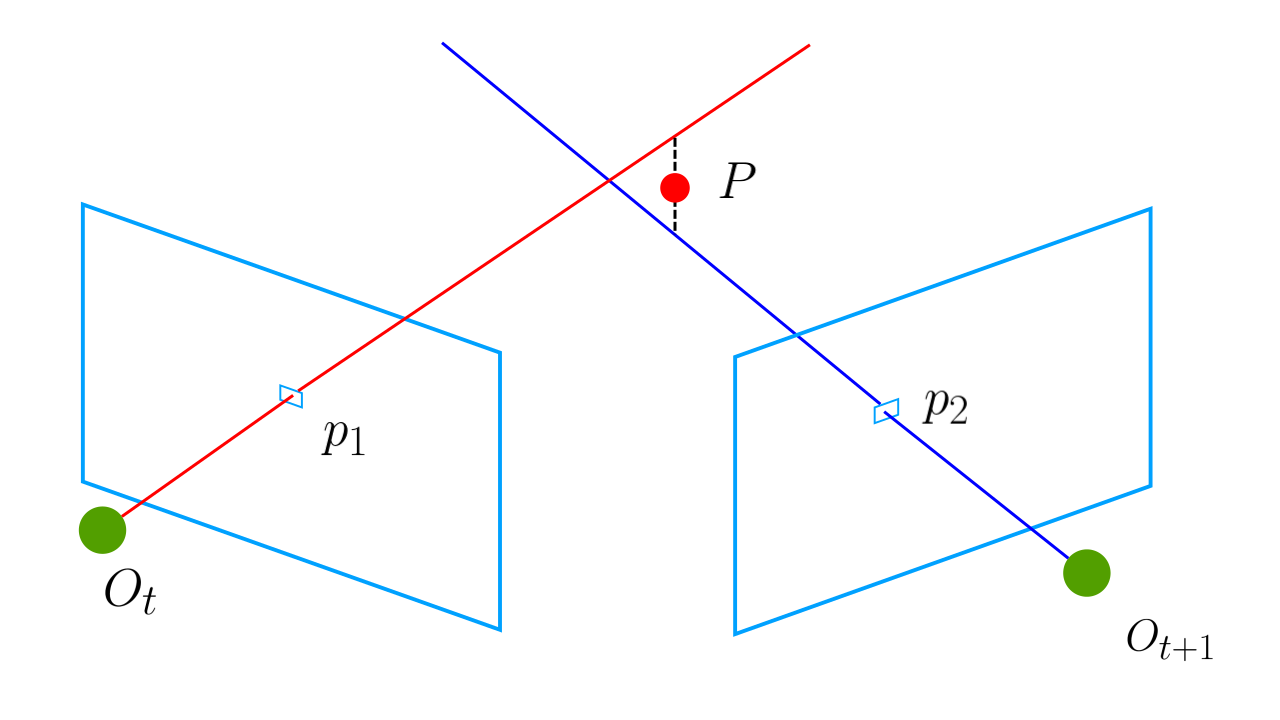
\includegraphics[width=0.9\linewidth]{vo1/triangularization}
	\caption{Use triangulation to estimate the depth.}
	\label{fig:triangluar}
\end{figure}

Triangulation refers to observing the same landmark point at different locations and determining the distance of the landmark point from the observed locations. Triangulation was first proposed by Gauss and used in metrology. It can also be applied to astronomy and geography. For example, we can estimate the distance to us from the angle of the star observed in different seasons. In SLAM, we mainly use triangulation to estimate the distance of pixels.

Similar to the previous section, consider the images $I_{1}$ and $I_{2}$, with the left image as a reference. The transform matrix to the right image is $\mathbf{T}$. The principal points of the camera are $O_{1}$ and $O_{2}$. The feature $p_{1}$ is in $I_{1}$, which corresponds to a feature $p_{2}$ in $I_{2}$. In theory, the straight line $O_{1}p_{1}$ and $O_{2}p_{2}$ will intersect at a point $P$ in the scene, which is the 3D map point. However, due to the noise, these two lines often fail to exactly intersect. Therefore, it can be solved in the sense of least-square.

According to the definition in epipolar geometry, let $\mathbf{x}_1, \mathbf{x}_2$ be the normalized coordinates of two feature points, then they satisfy:
\begin{equation}
s_2 \mathbf{x}_2 = s_1  \mathbf{R} \mathbf{x}_1 + \mathbf{t}.  
\end{equation}

Now we know the $\mathbf{R}$ and $\mathbf{t}$, we want to find the depth $s_1$ and $s_2$ of two feature points. Geometrically, you can find a 3D point on the ray $O_1 p_1$ to make its projection close to $\mathbf{p}_2$. Similarly, you can also find it on $O_2 p_2$ or in the middle of two lines. Different strategies correspond to different calculation methods, but the results are similar. For example, if we want to calculate $s_1$, we first multiply both sides of the above formula by $\mathbf{x}_2^\wedge$ to get:
\begin{equation}
\label{eq:x1tox2}
s_2 \mathbf{x}_2^\wedge \mathbf{x}_2 = 0 = s_1 \mathbf{x}_2^\wedge \mathbf{R} \mathbf{x}_1 + \mathbf{x}_2^\wedge \mathbf{t}. 
\end{equation}

The left side of this equation is zero, and the right side can be regarded as an equation of $s_1$, and $s_1$ can be obtained directly from it. With $s_1$, $s_2$ is also very easy to calculate. Thus, we get the depth of the points under the two frames and determine their spatial coordinates. Definitely, due to the existence of noise, our estimated $\mathbf{R}, \mathbf{t}$ may not exactly make the equation \eqref{eq:x1tox2} zero, so a more common approach is to find the least-square solution rather than a direct solution.

\section{Practice: Triangulation}
\subsection{Triangulation with OpenCV}
We demonstrate how to obtain the feature point's spatial position in the previous section through triangulation based on the camera pose solved by epipolar geometry. We will use the triangulation function provided by OpenCV here.

\begin{lstlisting}[language=c++,caption=slambook2/ch7/triangulation.cpp (part)]
void triangulation(
	const vector<key point> &key point_1,
	const vector<key point> &key point_2,
	const std::vector<DMatch> &matches,
	const Mat &R, const Mat &t,
	vector<Point3d> &points) {
	Mat T1 = (Mat_<float>(3, 4) <<
		1, 0, 0, 0,
		0, 1, 0, 0,
		0, 0, 1, 0);
	Mat T2 = (Mat_<float>(3, 4) <<
		R.at<double>(0, 0), R.at<double>(0, 1), R.at<double>(0, 2), t.at<double>(0, 0),
		R.at<double>(1, 0), R.at<double>(1, 1), R.at<double>(1, 2), t.at<double>(1, 0),
		R.at<double>(2, 0), R.at<double>(2, 1), R.at<double>(2, 2), t.at<double>(2, 0)
	);
	
	Mat K = (Mat_<double>(3, 3) << 520.9, 0, 325.1, 0, 521.0, 249.7, 0, 0, 1);
	vector<Point2f> pts_1, pts_2;
	for (DMatch m:matches) {
		// Convert pixel coordinates to camera coordinates
		pts_1.push_back(pixel2cam(key point_1[m.queryIdx].pt, K));
		pts_2.push_back(pixel2cam(key point_2[m.trainIdx].pt, K));
	}
	
	Mat pts_4d;
	cv::triangulatePoints(T1, T2, pts_1, pts_2, pts_4d);
	
	// Convert to non-homogeneous coordinates
	for (int i = 0; i < pts_4d.cols; i++) {
		Mat x = pts_4d.col(i);
		x /= x.at<float>(3, 0); // 归一化
		Point3d p(
			x.at<float>(0, 0),
			x.at<float>(1, 0),
			x.at<float>(2, 0)
		);
		points.push_back(p);
	}
}
\end{lstlisting}

Meanwhile, we can add the triangulation part to the main function and then draw each point's depth. Readers can run this program to view the triangulation results.

\subsection{Discussion}
Regarding triangulation, there is one more thing that must be noted.

Triangulation is caused by the \textit{translation}. Only when there is enough amount of translation, triangles in the epipolar geometry can be formed, and then the triangulation can be implemented. Therefore, triangulation cannot be used for pure rotation because the triangle does not exist in this case. Definitely, the real data is often not wholly equal to zero. In the presence of translation, we should also concern about the uncertainty of triangulation, which will lead to the triangulation contradiction.

As shown in \autoref{fig:triangulation-discuss}~, when the translation is small, the pixel's uncertainty will result in a more enormous depth uncertainty. That is to say, if the feature point moves by one pixel $\delta x$, the sight angle changes by an angle $\delta \theta$, then the measured depth will experience a difference of $\delta d$. It can be seen from the geometric relationship that when $\mathbf{t}$ is larger, $\delta d$ will be significantly smaller, meaning that when the translation is larger, the triangulation measurement will be more accurate at the same camera resolution. The quantitative analysis of the process can be proceeded by using the law of sine.

Therefore, to improve the accuracy of triangulation, one is to improve the accuracy of feature points extraction, which means to increase the image resolution, but this will cause the image to become larger and increase the computational cost. Another way is to increase the amount of translation. However, this will cause obvious changes in the image's appearance. For example, the box's side view initially blocked may be exposed, the lighting of the object changes, etc. Changes in appearance will make feature extraction and matching more difficult. In a nutshell, increasing the translation may lead to failure of matching; and if the translation is too small, the triangulation's accuracy is insufficient. This is the contradiction of triangulation. 

\begin{figure}[!ht]
	\centering
	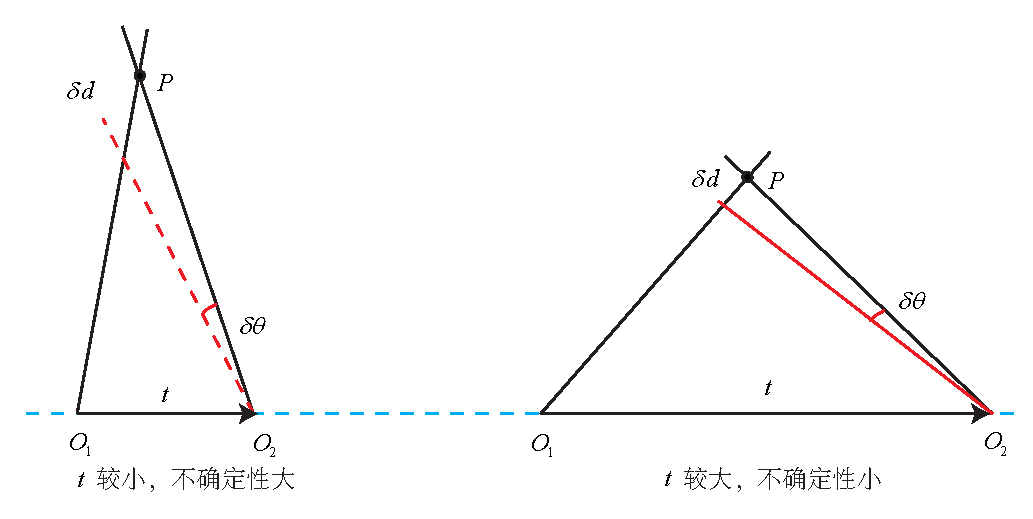
\includegraphics[width=1.0\linewidth]{vo1/triangulation-discuss.pdf}
	\caption{The contradiction of triangulation.}
	\label{fig:triangulation-discuss}
\end{figure}

In the monocular vision, since the image has no depth information, we have to wait for the feature points to be tracked for a few frames and then use triangulation to determine the new feature points' depth. This is also called delayed triangulation  {\cite{Davison2003}}. However, if the camera rotates in place, causing the parallax to be small, it is difficult to estimate the newly observed feature points' depth. This situation is common in robotics, as rotation is also a standard command for robots. In this case, monocular vision may suffer from tracking failures and incorrect scales.

Although this section only introduces the depth estimation of triangulation, we can also quantitatively calculate each feature point's location and uncertainty. Therefore, if we assume that the feature point obeys the Gaussian distribution and continuously observes it with the correct information, we can expect its variance will continue to decrease and even converge. This can be referred to as the depth filter. However, since its principle is more complicated, we will discuss it in later chapters \ref{cpt:12}. Next, we will discuss the estimation of camera motion from 3D-2D matching points and 3D-3D estimation methods.

\section{3D−2D:PnP}
PnP (Perspective-n-Point) is a method to solve 3D to 2D motion estimation. It describes how to estimate the camera's pose when the $n$ 3D space points and their projection positions are known. As mentioned earlier, the 2D-2D epipolar geometry method requires eight or more point pairs (take the eight-point method as an example), and there have problems with initialization, pure rotation, and scale. However, if the 3D position of one of the feature points in the two images is known, then we need at least three pairs (and at least one additional point to verify the result) to estimate the camera motion. The 3D position of the feature point can be determined by triangulation or the depth map of an RGB-D camera. Therefore, in binocular or RGB-D visual odometry, we can directly use PnP to estimate camera motion. While in the monocular case, initialization must be conducted before using PnP. The 3D-2D method does not require epipolar constraints and can obtain better motion estimation in a few matching points. It is the most important pose estimation method.

There are many ways to solve PnP problems, for example, P3P {\cite{GaoHouTangEtAl2003}}, direct linear transformation (DLT), EPnP (Efficient PnP) {\cite{LepetitMoreno-NoguerFua2008 }}, UPnP {\cite{Penate-SanchezAndrade-CettoMoreno-Noguer2013}}, etc. In addition, nonlinear optimization can be used to construct a least-square problem and iteratively solve it, which is commonly called the bundle adjustment. Let's look at DLT first, and then we will explain the bundle adjustment approach.

\subsection{Direct Linear Transformation}
Consider such a problem: we know the 3D positions of a point set and their projections in the camera, now we want to find the camera's pose. This problem can be used to solve the camera pose when a given map and image are given. If the 3D point is regarded as a point in another camera coordinate system, it can also solve the two cameras' relative motion problem. We will start with simple questions.

Consider a 3D spatial point $P$, its homogeneous coordinates are ${\mathbf{P}}=(X,Y,Z,1)^T$. In the image $I_{1}$, it is projected to the feature point ${\mathbf{x}}_{1}=(u_{1},v_{1},1)^T$(expressed as the normalized homogeneous coordinates). At this time, the pose of the camera $\mathbf{R}, \mathbf{t}$ is unknown. Similar to the solution of the homography matrix, we define the $3\times 4$ augmented matrix $[\mathbf{R}|\mathbf{t}]$, encoding rotation and translation information \footnote{This is different from the transformation matrix $\mathbf{T}$ in $\mathrm{SE}(3)$. }. We will write its expanded form as follows:
\begin{equation}
s
\begin{pmatrix}
u_{1} \\ v_{1} \\ 1
\end{pmatrix}
= \underbrace{
\begin{pmatrix}
t_{1} & t_{2} & t_{3} & t_{4}\\ 
t_{5} & t_{6} & t_{7} & t_{8}\\ 
t_{9} & t_{10} & t_{11} & t_{12}
\end{pmatrix}}_{[\mathbf{R}|\mathbf{t}]}
\begin{pmatrix}
X \\ Y \\ Z \\ 1
\end{pmatrix}.
\end{equation}

Eliminate $s$ with the last row to get two constraints:
\[
u_{1}=\frac{t_{1}X+t_{2}Y+t_{3}Z+t_{4}}{t_{9}X+t_{10}Y+t_{11}Z+t_{12}},\quad
v_{1}=\frac{t_{5}X+t_{6}Y+t_{7}Z+t_{8}}{t_{9}X+t_{10}Y+t_{11}Z+t_{12}}.
\]

To simplify the representation, define $\mathbf{T}$ as a row vector:
\[
\mathbf{t}_{1}=(t_{1},t_{2},t_{3},t_{4})^T,
\mathbf{t}_{2}=(t_{5},t_{6},t_{7},t_{8})^T,
\mathbf{t}_{3}=(t_{9},t_{10},t_{11},t_{12})^T.
\]

Now we have:
\[
\mathbf{t}_1^T\mathbf{P}-\mathbf{t}_3^T\mathbf{P} u_1=0,
\]
and
\[
\mathbf{t}_2^T\mathbf{P}-\mathbf{t}_3^T\mathbf{P} v_1=0.
\]

Please note that $\mathbf{t}$ is the variable to be determined. As you can see, each feature point provides two linear constraints on $\mathbf{t}$. Assuming there are a total of $N$ feature points, the following linear equations can be constructed:
\begin{equation}
\begin{pmatrix}
\mathbf{P}_{1}^T & 0 & -u_{1}\mathbf{P}_{1}^T	\\
0 & \mathbf{P}_{1}^T & -v_{1}\mathbf{P}_{1}^T	\\
\vdots & \vdots & \vdots			\\
\mathbf{P}_{N}^T & 0 & -u_{N}\mathbf{P}_{N}^T \\
0 & \mathbf{P}_{N}^T & -v_{N}\mathbf{P}_{N}^T
\end{pmatrix}
\begin{pmatrix}
\mathbf{t}_{1} \\ \mathbf{t}_{2} \\ \mathbf{t}_{3}
\end{pmatrix}
=0.
\end{equation}

Since $\mathbf{t}$ has a total dimension of 12, the linear solution of the matrix $\mathbf{T}$ can be achieved by at least six pairs of matching points. This method is called Direct Linear Transform (DLT). When the matching points are greater than 6 pairs, methods such as SVD can also be used to find the least-square solution of the overdetermined equation.

In the DLT solution, we directly regard the $\mathbf{T}$ matrix as 12 unknowns, ignoring the correlation between them. Because the rotation matrix $\mathbf{R} \in \mathrm{SO}(3)$, the solution obtained by DLT does not necessarily satisfy the $\mathrm{SE}(3)$ constraint. It is just a general matrix. The translation vector is easier to handle. It belongs to the vector space. For the rotation matrix $\mathbf{R}$, we must look for the best rotation matrix to approximate the matrix block of $3 \times 3$ on the left of $\mathbf{T}$ estimated by DLT. This can be done by QR decomposition  {\cite{Hartley2003, Chen1994}}, or it can be calculated like {\cite{Barfoot2016,Green1952}}:
\begin{equation}
\mathbf{R} \leftarrow {\left( {\mathbf{R}{\mathbf{R}^T}} \right)^{ - \frac{1}{2}}} \mathbf{R}.
\end{equation}
This can be seen as reprojecting the result from the matrix space onto the $\mathrm{SE}(3)$ manifold and converting it into two parts: rotation and translation.

What needs to be mentioned is that our $\mathbf{x}_1$ here uses normalized plane coordinates and neglects the influence of the intrinsic matrix $\mathbf{K}$. This is because $\mathbf{K}$ is usually assumed to be known in SLAM. Even if the intrinsic parameters are unknown, PnP can still be used to estimate the three quantities $\mathbf{K}, \mathbf{R}, \mathbf{t}$. However, due to the increase in the number of unknown variables, the result's quantity may be worse.

\subsection{P3P}
P3P is another way to solve PnP. It only uses 3 pairs of matching points and requires less data (this part refers to the \cite{web:p3p}).

P3P requires establishing geometric relationships of the given 3 points. Its input data is 3 pairs of 3D-2D matching points. Define 3D points as $A, B, C$, 2D points as $a, b, c$, where the point represented by the lowercase letter is the projection of the point on the camera image plane represented by the corresponding uppercase letter, as shown in \autoref{fig:p3p}~. Also, P3P needs a pair of verification points to select the correct one from the possible solutions (similar to epipolar geometry). Denote the verification point pair as $D-d$ and the principal camera point as $O$. Suppose that $A, B, C$ are in the world coordinate frame, not the camera coordinate. Once the coordinates of the 3D point in the camera coordinate system can be calculated, we get the 3D−3D corresponding point and convert the PnP problem to the ICP problem.

\begin{figure}[!ht]
	\centering
	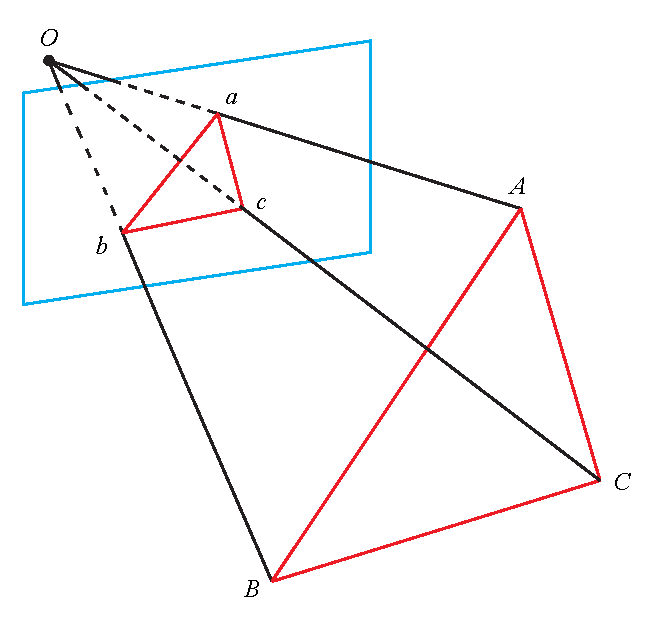
\includegraphics[width=0.54\linewidth]{vo1/p3p.pdf}
	\caption{The P3P problem.}
	\label{fig:p3p}
\end{figure}

Obviously, there is a relationship between triangles:
\begin{equation}
\Delta Oab - \Delta OAB, \quad \Delta Obc - \Delta OBC, \quad \Delta Oac - \Delta OAC.
\end{equation}

Consider the relationship between $Oab$ and $OAB$. Using the law of cosines, there are:
\begin{equation}
O{A^2} + O{B^2} - 2OA \cdot OB \cdot \cos \left\langle a,b \right \rangle  = A{B^2}.
\end{equation}

The other two triangles have similar properties, so we further get:
\begin{equation}
\begin{array}{l}
O{A^2} + O{B^2} - 2OA \cdot OB \cdot \cos \left\langle a,b \right \rangle  = A{B^2}\\
O{B^2} + O{C^2} - 2OB \cdot OC \cdot \cos \left\langle b,c \right \rangle  = B{C^2}\\
O{A^2} + O{C^2} - 2OA \cdot OC \cdot \cos \left\langle a,c \right \rangle  = A{C^2}.
\end{array}
\end{equation}

Divide all the above three equations by $OC^2$ on both sides, and let $x=OA/OC, y=OB/OC$, we get:
\begin{equation}
\begin{array}{l}
{x^2} + {y^2} - 2xy\cos \left\langle a,b \right \rangle  = A{B^2}/O{C^2}\\
{y^2} + {1^2} - 2y\cos \left\langle b,c \right \rangle  = B{C^2}/O{C^2}\\
{x^2} + {1^2} - 2x\cos \left\langle a,c \right \rangle  = A{C^2}/O{C^2}.
\end{array}
\end{equation}

Let $v = AB^2/OC^2, uv = BC^2/OC^2, wv = AC^2/OC^2$, then we have:
\begin{equation}
\begin{array}{l}
{x^2} + {y^2} - 2xy\cos \left\langle a,b \right \rangle  - v = 0\\
{y^2} + {1^2} - 2y\cos \left\langle b,c \right \rangle  - uv = 0\\
{x^2} + {1^2} - 2x\cos \left\langle a,c \right \rangle  - wv = 0.
\end{array}
\end{equation}

Move $v$ in the first equation to the right side, and combine it with the other two equations, we have:
\begin{equation}
\begin{array}{l}
\left( {1 - u} \right){y^2} - u{x^2} - 2 \cos \left\langle b,c \right \rangle y + 2uxy\cos \left\langle a,b \right \rangle  + 1 = 0 \\
\left( {1 - w} \right){x^2} - w{y^2} - 2 \cos \left\langle a,c \right \rangle x + 2wxy\cos \left\langle a,b \right \rangle  + 1 = 0.
\end{array}
\end{equation}

Please distinguish the known from the unknown quantities in these equations. Since we know the positions of the 2D points in the image, the 3 cosine angles $\cos \left \langle a,b \right \rangle$, $\cos \left\langle b,c \right \rangle$, $\cos \left \langle a,c \right \rangle$ can be calculated. Meanwhile, $u=BC^2/AB^2, w=AC^2/AB^2$ can be calculated by the coordinates of $A, B, C$ in the world frame. Transforming to the camera frame does not change the ratio. The $x$ and $y$ are unknown and will change as the camera moves. Therefore, the equations are quadratic equations about two unknowns $x, y$. Analytically solving the equations is complicated and requires Wu's elimination method. It will not be introduced here. Interested readers could refer to the literature \cite{GaoHouTangEtAl2003}. Analogous to the case of decomposing $\mathbf{E}$, this equation may get 4 solutions at most. Still, we can use the verification points to select the most probable solution and get the 3D of $A, B, C$ in the camera frame. Then, based on the 3D−3D point pair, the camera movement $\mathbf{R}, \mathbf{t}$ can be calculated, which will be introduced in section 7.9.

From the principle of P3P to solve PnP, we use the triangle relationships to solve the 3D coordinates of the projection points $a, b, c$ in the camera frame, and finally convert the problem into a 3D to 3D pose estimation problem. As we will see later, it is easy to solve the 3D-3D pose with matching information, so this idea is very effective. Some other methods, such as EPnP, also adopted this idea. However, P3P also has some deficiencies:

\begin{enumerate}
	\item P3P only includes the information of 3 points. When the given matched points are more than 3, it is difficult to use more information.
	\item If the 3D point or 2D point is affected by noise or a mismatch, the algorithm goes into trouble.
\end{enumerate}

People also proposed many other methods, such as EPnP, UPnP, and so on. They use more information and iteratively optimize the camera pose to eliminate noise as much as possible. However, compared to P3P, the principles are more complicated, so we recommend that readers read the original papers or understand the PnP process by practice. In SLAM, the usual approach is to first estimate the camera pose using P3P/EPnP and then construct a least-squares optimization problem to adjust the estimated values (bundle adjustment). When the camera motion is sufficiently continuous, or you can also assume that the camera does not move or move at a constant speed, you can use the estimated values as the initial values for optimization. Next, we look at the PnP problem from the perspective of nonlinear optimization.

\subsection{Solve PnP by Minimizing the Reprojection Error}
\label{sec:BA-vo1}
Other than the linear method, we can also construct the PnP problem as a nonlinear least-square problem about reprojection errors. This will use the knowledge from the chapters \ref{cpt:4} and \ref{cpt:5} of this book. The linear method mentioned above is often divided into many steps, such as estimating the camera pose first and then the point's position. While nonlinear optimization treats them as optimization variables and optimizes them together. This is a very general solution method. We can use it to optimize the results given by PnP or ICP. This type of problem, putting the camera and 3D points together to minimize, is generally referred to as bundle adjustment \footnote{The meaning of BA in different documents and contexts are not exactly the same. Some people only refer to problems that minimize the reprojection errors as BA, while others have a broader definition of BA. Even if the BA has only one camera, it can be called BA. I personally prefer the broader definition, so the method of calculating PnP here is also called BA.}.

We can build a bundle adjustment problem in PnP to optimize the camera pose. If the camera is moving continuously (as in most SLAM processes), we can also use BA directly to solve the camera pose. In this section, we will give the basic two-view form of this problem and then discuss the larger-scale BA problem in lecture \ref{cpt:9}.

Suppose we have $n$ 3D space points $P$ and their projection $p$, we want to calculate the pose $\mathbf{R}, \mathbf{t}$ of the camera. Suppose the coordinates of a point are $\mathbf{P}_i=[X_i,Y_i,Z_i]^T$, and their projected pixel coordinates are $\mathbf{u}_i=[u_i,v_i]^ \mathrm{T}$. According to \ref{cpt:5}, the relationship between the 2D pixel position and the 3D spatial position is:
\begin{equation}
s_i \left[ 
\begin{array}{l}
u_i \\ v_i \\ 1
\end{array}
\right] = \mathbf{K} \mathbf{T} \left[ 
\begin{array}{l}
X_i \\ Y_i \\ Z_i \\ 1
\end{array} \right]  .
\end{equation}
Or in the matrix form:
\[
{{s_i {\mathbf{u}}_i} = \mathbf{K} \mathbf{T} \mathbf{P}}_i.
\]

This equation includes a conversion from homogeneous coordinates to non-homogeneous coordinates implicitly. Or we can also use $\mathbf{R}\mathbf{P}+\mathbf{t}$. Now, due to the unknown camera pose and the noise of the observation points, there is a residual in the equation. Therefore, we sum up the residuals, construct a least-square problem, and then minimize it to find the most possible camera pose:
\begin{equation}
{\mathbf{T}^*} = \arg \mathop {\min }\limits_{\mathbf{T}}  \frac{1}{2}\sum\limits_{i = 1}^n {\left\| {{{\mathbf{u}}_i} - \frac{1}{s_i} \mathbf{K}\mathbf{T}{\mathbf{P}}_i} \right\|_2^2} .
\end{equation}

The residual term is the error of the projected position and the observed position, which is called the reprojection error. With homogeneous coordinates, this error has three dimensions. However, since the last dimension of ${\mathbf{u}}$ is 1, the error of this dimension is always zero, so we normally use non-homogeneous coordinates. Therefore, the error has only 2 dimensions. As shown in \autoref{fig:reprojection}~, we know that $p_1$ and $p_2$ are projections of the same space point $P$ through feature matching, but we don't know the pose of the camera. In the initial value, there is a certain distance between the projection of $P \hat{p}_2$ and the observed $p_2$. So we adjusted the pose of the camera to make this distance smaller. However, since this adjustment needs to consider many points, the goal is to reduce the overall error, and the error of each point usually can not be exactly zero.

\begin{figure}[!htp]
	\centering
	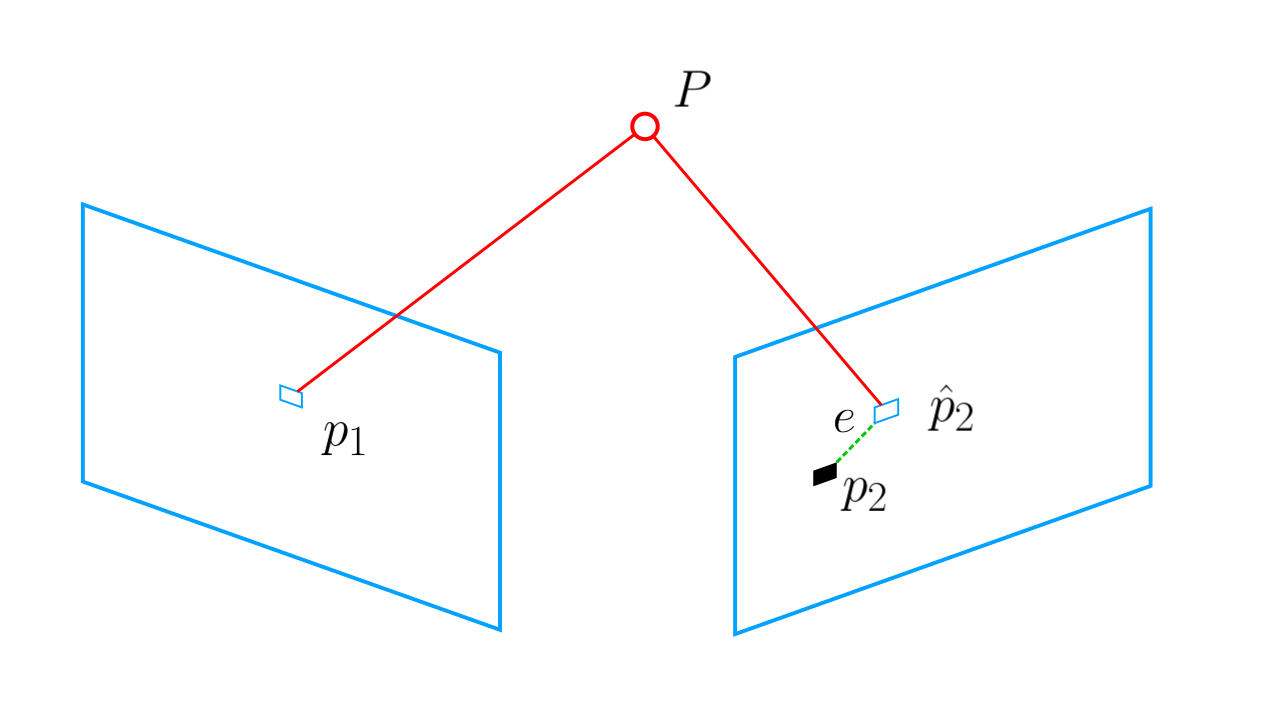
\includegraphics[width=0.8\linewidth]{vo1/reprojection}
	\caption{The reprojection error.}
	\label{fig:reprojection}
\end{figure}

We have already discussed the least-square optimization problem in chapter \ref{cpt:6}. Using Lie algebra, we can construct an unconstrained optimization problem on the manifold, easily solved using optimization algorithms such as the Gauss-Newton method and Levenberg-Marquardt method. However, we need to calculate the derivative of each error term with respect to the optimization variable, which is also the linearization:
\begin{equation}
\mathbf{e}( \mathbf{x} + \Delta \mathbf{x} ) \approx \mathbf{e}(\mathbf{x}) + \mathbf{J} ^T\Delta \mathbf{x}.
\end{equation}

The form of $\mathbf{J}^T$ is worth discussing. Definitely, we can use numerical derivatives, but if we can derive an analytical form, we will prefer the analytical derivatives. Now, $\mathbf{e}$ is the pixel coordinate error (2-d) and $\mathbf{x}$ is the camera pose (6-d), $\mathbf{J}^T$ is a matrix of $2 \times 6$. Let's derive the form of $\mathbf{J}^T$.

We have introduced how to use the perturbation model to find the pose variable's derivative (chapter \ref{cpt:4}). First, define the coordinates of the space point in the camera frame as $\mathbf{P}'$, and take out the first 3 dimensions:
\begin{equation}
\mathbf{P}' = \left( \mathbf{T}{\mathbf{P}} \right)_{1:3}= [X', Y', Z']^T.
\end{equation}

Then, the camera projection model with respect to $\mathbf{P}'$ is:
\begin{equation}
s {\mathbf{u}} = \mathbf{K} \mathbf{P}'.
\end{equation}

Expand it:
\begin{equation}
\left[ \begin{array}{l}
su\\
sv\\
s
\end{array} \right] = \left[ {\begin{array}{*{20}{c}}
	{{f_x}}&0&{{c_x}}\\
	0&{{f_y}}&{{c_y}}\\
	0&0&1
	\end{array}} \right]\left[ \begin{array}{l}
X'\\
Y'\\
Z'
\end{array} \right].
\end{equation}

Use the third row to eliminate $s$ (actually it is the distance of $\mathbf{P}'$), we get:
\begin{equation}
\label{eq:uv2xyz}
u = {f_x}\frac{{X'}}{{Z'}} + {c_x}, \quad v = {f_y}\frac{{Y'}}{{Z'}} + {c_y}.
\end{equation}

This is consistent with the camera model described in \ref{cpt:5}. When we find the error, we can compare the $u, v$ here with the measured value to find the difference. After defining the intermediate variables, we left multiply $\mathbf{T}$ by a disturbance quantity $\delta \boldsymbol{\xi}$, and then consider the derivative of the change of $\mathbf{e}$ with respect to the disturbance quantity. Using the chain rule, it is:
\begin{equation}
\frac{{\partial \mathbf{e}}}{{\partial \delta \boldsymbol{\xi} }} = \mathop {\lim }\limits_{\delta \boldsymbol{\xi}  \to 0} \frac{{\mathbf{e}\left( {\delta \boldsymbol{\xi}  \oplus \boldsymbol{\xi} } \right)-\mathbf{e}(\boldsymbol{\xi})}}{{\delta \boldsymbol{\xi} }}  = \frac{{\partial \mathbf{e}}}{{\partial \mathbf{P}'}}\frac{{\partial \mathbf{P}'}}{{\partial \delta \boldsymbol{\xi} }}.
\end{equation}

Here $\oplus$ refers to the disturbance left multiplication in Lie algebra. The first item is the derivative of the error with respect to the projection point. The relationship between the variables is in the equation \eqref{eq:uv2xyz}, and it is easy to get:
\begin{equation}
\frac{{\partial \mathbf{e}}}{{\partial \mathbf{P}'}} = -\left[ 
{\begin{array}{*{20}{c}}
	{\frac{{\partial u}}{{\partial X'}}}&{\frac{{\partial u}}{{\partial Y'}}}&{\frac{{\partial u}}{{\partial Z'}}}\\
	{\frac{{\partial v}}{{\partial X'}}}&{\frac{{\partial v}}{{\partial Y'}}}&{\frac{{\partial v}}{{\partial Z'}}}
	\end{array}} \right] 
= - \left[ {\begin{array}{*{20}{c}}
	{\frac{{{f_x}}}{Z'}}&0&{ - \frac{{{f_x}X'}}{{{Z'^2}}}}\\
	0&{\frac{{{f_y}}}{Z'}}&{ - \frac{{{f_y}Y'}}{Z'^2}}
\end{array}} \right].
\end{equation}

The second term is the derivative of the transformed point with respect to the Lie algebra. According to the section \ref{sec:se3-diff}, we get:
\begin{equation}
\frac{{\partial \left( \mathbf{TP} \right)}}{{\partial \delta \boldsymbol{\xi} }} = {\left( \mathbf{TP} \right)^ \odot } = \left[ 
\begin{array}{*{20}{cc}}
\mathbf{I} &- \mathbf{P}'^ \wedge \\
\mathbf{0}^T &\mathbf{0}^T 
\end{array}
\right].
\end{equation}

In the definition of $\mathbf{P}'$, we took out the first 3 dimensions, so we get:
\begin{equation}
\frac{{\partial \mathbf{P}'}}{{\partial \delta \boldsymbol{\xi} }} = \left[ { \mathbf{I}, - {\mathbf{P}'^ \wedge }} \right].
\end{equation}

Multiply these two items together, we get the $2 \times 6$ Jacobian matrix:
\begin{equation}
\label{eq:jacob-uv2xi}
\frac{{\partial \mathbf{e}}}{{\partial \delta \boldsymbol{\xi} }} = - \left[ {\begin{array}{*{20}{c}}
	{\frac{{{f_x}}}{Z'}}&0&{ - \frac{{{f_x}X'}}{{{Z'^2}}}}&{ - \frac{{{f_x}X'Y'}}{{{Z'^2}}}}&{{f_x} + \frac{{{f_x}{X'^2}}}{{{Z'^2}}}}&{ - \frac{{{f_x}Y'}}{Z'}}\\
	0&{\frac{{{f_y}}}{Z'}}&{ - \frac{{{f_y}Y'}}{{{Z'^2}}}}&{ - {f_y} - \frac{{{f_y}{Y'^2}}}{{{Z'^2}}}}&{\frac{{{f_y}X'Y'}}{{{Z'^2}}}}&{\frac{{{f_y}X'}}{Z'}}
	\end{array}} \right].
\end{equation}

This Jacobian matrix describes the first-order derivative of the reprojection error with respect to the left perturbation model. We keep the negative sign in front of it because the error is defined by the observed value minus the predicted value. It can also be reversed and defined in the form of the predicted value minus the observed value. In that case, just remove the negative sign in front. Besides, if the definition of $\mathfrak{se}(3)$ is a rotation followed by translation, just swap the first 3 columns and the last 3 columns of this Jacobian matrix.

On top of optimizing the pose, we want to optimize the spatial position of the feature points. Therefore, we also need to discuss the derivative of $\mathbf{e}$ with respect to the space point $\mathbf{P}$. Fortunately, this derivative matrix is relatively easy. Still using the chain rule, there are:
\begin{equation}
\frac{{\partial \mathbf{e}}}{{\partial \mathbf{P} }} = \frac{{\partial \mathbf{e}}}{{\partial \mathbf{P}'}}\frac{{\partial \mathbf{P}'}}{{\partial \mathbf{P} }}.
\end{equation}

The first item has been deduced before, and the second item is defined as:
\[
\mathbf{P}'= (\mathbf{T} \mathbf{P})_{1:3} = \mathbf{R} \mathbf{P} + \mathbf{t},
\]
So only $\mathbf{R}$ is left in the derivative:
\begin{equation}
\label{eq:jacob-uv2P}
\frac{{\partial \mathbf{e}}}{{\partial \mathbf{P} }} = -\left[ 
\begin{array}{*{20}{c}}
	\frac{f_x}{Z'} & 0 &- \frac{f_x X'}{Z'^2} \\
	0 & \frac{f_y}{Z'} & - \frac{f_y Y'}{Z'^2}
\end{array} \right] \mathbf{R}.
\end{equation}

We have derived the two Jacobian matrices of the observation camera equation with respect to the camera pose and feature points. They are very important to provide gradient directions in the optimization and guide the iteration of optimization.

\section{Practice: Solving PnP}
\subsection{Use EPnP to Solve the Pose}
In the following, we will have a deeper understanding of the PnP process through practice. First, we demonstrate how to use OpenCV's EPnP to solve the PnP problem and then solve it again through nonlinear optimization. In the second edition of the book, we also add a handwriting optimization practice. Since PnP needs to use 3D points, to avoid the trouble of initialization, we use the depth map (1_depth.png) in the RGB-D camera as the 3D position of the feature points. First look at the PnP function provided by OpenCV:

\begin{lstlisting}[language=c++,caption=slambook2/ch7/pose_estimation_3d2d.cpp (part)]
int main( int argc, char** argv ) {
   Mat r, t;
   solvePnP(pts_3d, pts_2d, K, Mat(), r, t, false); // Call OpenCV's PnP, you can choose from EPNP, DLS and other methods
   Mat R;
   cv::Rodrigues(r, R); // r is in the form of rotation vector, and converted to a rotation matrix by Rodrigues formula
   cout << "R=" << endl << R << endl;
   cout << "t=" << endl << t << endl;
}
\end{lstlisting}

In the example, after obtaining the matched feature points, we get their depth in the depth map of the first image and find their spatial position. Taking this spatial position as a 3D point and then taking the second image's pixel position as a 2D observation, we call EPnP to solve the PnP problem. The program output is as follows:

\begin{lstlisting}[language=sh,caption=Terminal output:]
% build/pose_estimation_3d2d 1.png 2.png d1.png d2.png
-- Max dist : 95.000000 
-- Min dist : 4.000000 
In total, we get 79 set of feature points
3d-2d pairs: 76
R=
[0.9978662025826269, -0.05167241613316376, 0.03991244360207524;
0.0505958915956335, 0.998339762771668, 0.02752769192381471;
-0.04126860182960625, -0.025449547736074, 0.998823919929363]
t=
[-0.1272259656955879;
-0.007507297652615337;
0.06138584177157709]
\end{lstlisting}

Readers can compare $\mathbf{R},\mathbf{t}$ solved in the previous 2D-2D case to see the difference. It can be seen that when 3D information is involved, the estimated $\mathbf{R}$ is almost the same, while the $\mathbf{t}$ is quite different. This is due to the inclusion of depth information. However, since the depth map collected by Kinect has some noise, the 3D points here are not accurate. In a larger-scale BA, we would like to optimize the pose and all 3D feature points at the same time.


\subsection{Pose Estimation from Scratch}
The following demonstrates how to use nonlinear optimization to calculate the camera pose. We first write a PnP of the Gauss-Newton method and then demonstrate how to solve it by \textit{g2o}.
\begin{lstlisting}[language=c++,caption=slambook2/ch7/pose_estimation_3d2d.cpp (part)]
void bundleAdjustmentGaussNewton(
const VecVector3d &points_3d,
const VecVector2d &points_2d,
const Mat &K,
Sophus::SE3d &pose) {
	typedef Eigen::Matrix<double, 6, 1> Vector6d;
	const int iterations = 10;
	double cost = 0, lastCost = 0;
	double fx = K.at<double>(0, 0);
	double fy = K.at<double>(1, 1);
	double cx = K.at<double>(0, 2);
	double cy = K.at<double>(1, 2);
	
	for (int iter = 0; iter < iterations; iter++) {
		Eigen::Matrix<double, 6, 6> H = Eigen::Matrix<double, 6, 6>::Zero();
		Vector6d b = Vector6d::Zero();
		
		cost = 0;
		// compute cost
		for (int i = 0; i < points_3d.size(); i++) {
			Eigen::Vector3d pc = pose * points_3d[i];
			double inv_z = 1.0 / pc[2];
			double inv_z2 = inv_z * inv_z;
			Eigen::Vector2d proj(fx * pc[0] / pc[2] + cx, fy * pc[1] / pc[2] + cy);
			Eigen::Vector2d e = points_2d[i] - proj;
			cost += e.squaredNorm();
			Eigen::Matrix<double, 2, 6> J;
			J << -fx * inv_z,
			0,
			fx * pc[0] * inv_z2,
			fx * pc[0] * pc[1] * inv_z2,
			-fx - fx * pc[0] * pc[0] * inv_z2,
			fx * pc[1] * inv_z,
			0,
			-fy * inv_z,
			fy * pc[1] * inv_z,
			fy + fy * pc[1] * pc[1] * inv_z2,
			-fy * pc[0] * pc[1] * inv_z2,
			-fy * pc[0] * inv_z;
			
			H += J.transpose() * J;
			b += -J.transpose() * e;
		}
		
		Vector6d dx;
		dx = H.ldlt().solve(b);
		
		if (isnan(dx[0])) {
			cout << "result is nan!" << endl;
			break;
		}
		
		if (iter > 0 && cost >= lastCost) {
			// cost increase, update is not good
			cout << "cost: " << cost << ", last cost: " << lastCost << endl;
			break;
		}
		
		// update your estimation
		pose = Sophus::SE3d::exp(dx) * pose;
		lastCost = cost;
		
		cout << "iteration " << iter << " cost=" << cout.precision(12) << cost << endl;
		if (dx.norm() < 1e-6) {
			// converge
			break;
		}
	}
	
	cout << "pose by g-n: \n" << pose.matrix() << endl;
}
\end{lstlisting}

In this function, we implement a simple Gauss-Newton iterated optimization based on the previous derivation. Then we will compare the efficiency of OpenCV, handwritten implementation, and the \textit{g2o} implementation.

\subsection{Optimization by \textit{g2o}}
After handwriting the optimization process, let's look at how to achieve the same functionality using the library \textit{g2o} (it is similar to Ceres). The basic knowledge of \textit{g2o} has been introduced in lecture \ref{cpt:6}. Before using \textit{g2o}, we have to model the problem as a graph optimization problem, as shown in \autoref{fig:ba-graph}~.

\begin{figure}[!htp]
	\centering
	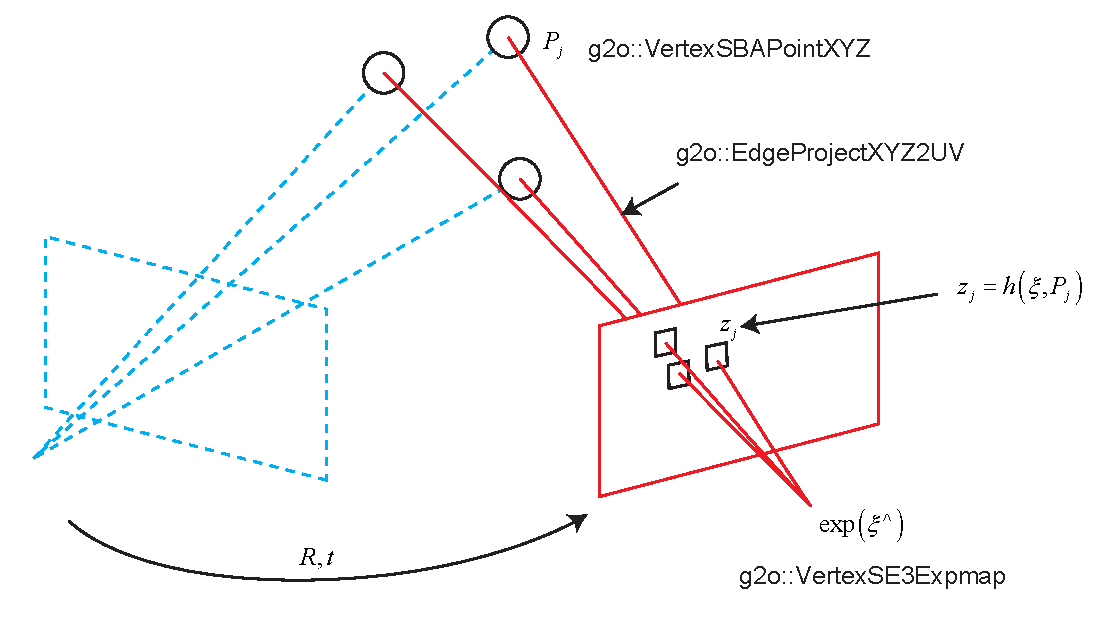
\includegraphics[width=0.9\linewidth]{vo1/ba-graph}
	\caption{PnP's graph structure.}
	\label{fig:ba-graph}
\end{figure}

In this graph optimization, the nodes and edges are defined as follows:
\begin{enumerate}
	\item \textbf{Node}: The pose of the second camera $\mathbf{T} \in \mathrm{SE}(3)$.
	\item \textbf{Edge}: The projection of each 3D point in the second camera, described by the observation equation:
	\[
	\mathbf{z}_j = h(\mathbf{T}, \mathbf{P}_{j}).
	\]
\end{enumerate}

Since the pose of the first camera is fixed to identity, we excluded it from the optimization variables. But in normal cases, we will consider estimations of many cameras. Now we estimate the second camera pose based on a set of 3D points and the 2D projection in the second image. We drew the first camera as a dotted line to indicate that we don't want to consider it.

g2o provides many nodes and edges about BA. For example, \textit{g2o/\\types/sba/types\_six\_dof\_expmap.h} provides nodes and edges expressed by Lie algebra. In the second edition of the book, we implement a VertexPose vertex and EdgeProjection edge ourselves, as follows:
\begin{lstlisting}[language=c++,caption=slambook2/ch7/pose_estimation_3d2d.cpp (part)]
/// vertex and edges used in g2o ba
class VertexPose : public g2o::BaseVertex<6, Sophus::SE3d> {
	public:
	EIGEN_MAKE_ALIGNED_OPERATOR_NEW;
	
	virtual void setToOriginImpl() override {
		_estimate = Sophus::SE3d();
	}
	
	/// left multiplication on SE3
	virtual void oplusImpl(const double *update) override {
		Eigen::Matrix<double, 6, 1> update_eigen;
		update_eigen << update[0], update[1], update[2], update[3], update[4], update[5];
		_estimate = Sophus::SE3d::exp(update_eigen) * _estimate;
	}
	
	virtual bool read(istream &in) override {}
	
	virtual bool write(ostream &out) const override {}
};

class EdgeProjection : public g2o::BaseUnaryEdge<2, Eigen::Vector2d, VertexPose> {
	public:
	EIGEN_MAKE_ALIGNED_OPERATOR_NEW;
	
	EdgeProjection(const Eigen::Vector3d &pos, const Eigen::Matrix3d &K) : _pos3d(pos), _K(K) {}
	
	virtual void computeError() override {
		const VertexPose *v = static_cast<VertexPose *> (_vertices[0]);
		Sophus::SE3d T = v->estimate();
		Eigen::Vector3d pos_pixel = _K * (T * _pos3d);
		pos_pixel /= pos_pixel[2];
		_error = _measurement - pos_pixel.head<2>();
	}
	
	virtual void linearizeOplus() override {
		const VertexPose *v = static_cast<VertexPose *> (_vertices[0]);
		Sophus::SE3d T = v->estimate();
		Eigen::Vector3d pos_cam = T * _pos3d;
		double fx = _K(0, 0);
		double fy = _K(1, 1);
		double cx = _K(0, 2);
		double cy = _K(1, 2);
		double X = pos_cam[0];
		double Y = pos_cam[1];
		double Z = pos_cam[2];
		double Z2 = Z * Z;
		_jacobianOplusXi
		<< -fx / Z, 0, fx * X / Z2, fx * X * Y / Z2, -fx - fx * X * X / Z2, fx * Y / Z,
		0, -fy / Z, fy * Y / (Z * Z), fy + fy * Y * Y / Z2, -fy * X * Y / Z2, -fy * X / Z;
	}
	
	virtual bool read(istream &in) override {}
	
	virtual bool write(ostream &out) const override {}
	
	private:
	Eigen::Vector3d _pos3d;
	Eigen::Matrix3d _K;
};
\end{lstlisting}

This implements vertex update and edge error calculation. The following is to combine them into a graph optimization problem:
\begin{lstlisting}[language=c++,caption=slambook2/ch7/pose_estimation_3d2d.cpp (part)]
void bundleAdjustmentG2O(
const VecVector3d &points_3d,
const VecVector2d &points_2d,
const Mat &K,
Sophus::SE3d &pose) {
	// Build graph optimization, first let's define g2o
	typedef g2o::BlockSolver<g2o::BlockSolverTraits<6, 3>> BlockSolverType;  // pose is 6, landmark is 3
	typedef g2o::LinearSolverDense<BlockSolverType::PoseMatrixType> LinearSolverType;
	// Gradient descent method, you can choose from GN, LM, DogLeg
	auto solver = new g2o::OptimizationAlgorithmsGaussNewton(
		g2o::make_unique<BlockSolverType>(g2o::make_unique<LinearSolverType>()));
	g2o::SparseOptimizer optimizer;     // Graph model
	optimizer.setAlgorithm(solver);   // Set up the solver
	optimizer.setVerbose(true);       // Turn on verbose output for debugging
	
	// vertex
	VertexPose *vertex_pose = new VertexPose(); // camera vertex_pose
	vertex_pose->setId(0);
	vertex_pose->setEstimate(Sophus::SE3d());
	optimizer.addVertex(vertex_pose);
	
	// K
	Eigen::Matrix3d K_eigen;
	K_eigen <<
	K.at<double>(0, 0), K.at<double>(0, 1), K.at<double>(0, 2),
	K.at<double>(1, 0), K.at<double>(1, 1), K.at<double>(1, 2),
	K.at<double>(2, 0), K.at<double>(2, 1), K.at<double>(2, 2);
	
	// edges
	int index = 1;
	for (size_t i = 0; i < points_2d.size(); ++i) {
		auto p2d = points_2d[i];
		auto p3d = points_3d[i];
		EdgeProjection *edge = new EdgeProjection(p3d, K_eigen);
		edge->setId(index);
		edge->setVertex(0, vertex_pose);
		edge->setMeasurement(p2d);
		edge->setInformation(Eigen::Matrix2d::Identity());
		optimizer.addEdge(edge);
		index++;
	}
	
	chrono::steady_clock::time_point t1 = chrono::steady_clock::now();
	optimizer.setVerbose(true);
	optimizer.initializeOptimization();
	optimizer.optimize(10);
	chrono::steady_clock::time_point t2 = chrono::steady_clock::now();
	chrono::duration<double> time_used = chrono::duration_cast<chrono::duration<double>>(t2 - t1);
	cout << "optimization costs time: " << time_used.count() << " seconds." << endl;
	cout << "pose estimated by g2o =\n" << vertex_pose->estimate().matrix() << endl;
	pose = vertex_pose->estimate();
}
\end{lstlisting}

The program is similar to \textit{g2o} in lecture 6. We first declare the \textit{g2o} graph optimizer and configure the solver and gradient descent method. Then, based on the estimated feature points, we put the pose and spatial points into the graph. Finally, the optimization function is called. The partial output of the run is as follows:

\begin{lstlisting}[language=sh,caption=Terminal output:]
./build/pose_estimation_3d2d 1.png 2.png 1_depth.png 2_depth.png
-- Max dist : 95.000000 
-- Min dist : 4.000000 
In total, we get 79 set of feature points
3d-2d pairs: 76
solve pnp in opencv cost time: 0.000332991 seconds.
R=
[0.9978662025826269, -0.05167241613316376, 0.03991244360207524;
0.0505958915956335, 0.998339762771668, 0.02752769192381471;
-0.04126860182960625, -0.025449547736074, 0.998823919929363]
t=
[-0.1272259656955879;
-0.007507297652615337;
0.06138584177157709]
calling bundle adjustment by gauss newton
iteration 0 cost=645538.1857253
iteration 1 cost=12750.239874896
iteration 2 cost=12301.774589343
iteration 3 cost=12301.427574651
iteration 4 cost=12301.426806652
pose by g-n: 
0.99786618832  -0.0516873580423    0.039893448423   -0.127218696289
0.0506143671126    0.998340854865   0.0274540224544 -0.00738695798083
-0.0412462852904  -0.0253762590968    0.998826706403   0.0617019263823
0                 0                 0                 1
solve pnp by gauss newton cost time: 0.000159492 seconds.
calling bundle adjustment by g2o
iteration= 0	 chi2= 413.390599	 time= 2.7291e-05	 cumTime= 2.7291e-05	 edges= 76	 schur= 0	 lambda= 79.000412	 levenbergIter= 1
iteration= 1	 chi2= 301.367030	 time= 1.47e-05	 cumTime= 4.1991e-05	 edges= 76	 schur= 0	 lambda= 26.333471	 levenbergIter= 1
iteration= 2	 chi2= 301.365779	 time= 1.7794e-05	 cumTime= 5.9785e-05	 edges= 76	 schur= 0	 lambda= 17.555647	 levenbergIter= 1
iteration= 3	 chi2= 301.365779	 time= 1.4875e-05	 cumTime= 7.466e-05	 edges= 76	 schur= 0	 lambda= 11.703765	 levenbergIter= 1
iteration= 4	 chi2= 301.365779	 time= 1.3132e-05	 cumTime= 8.7792e-05	 edges= 76	 schur= 0	 lambda= 7.802510	 levenbergIter= 1
iteration= 5	 chi2= 301.365779	 time= 2.0379e-05	 cumTime= 0.000108171	 edges= 76	 schur= 0	 lambda= 41.613386	 levenbergIter= 3
iteration= 6	 chi2= 301.365779	 time= 3.4186e-05	 cumTime= 0.000142357	 edges= 76	 schur= 0	 lambda= 2859650082279.672363	 levenbergIter= 8
optimization costs time: 0.000763649 seconds.
pose estimated by g2o =
0.997866202583  -0.0516724161336   0.0399124436024   -0.127225965696
0.050595891596    0.998339762772   0.0275276919261 -0.00750729765631
-0.04126860183  -0.0254495477384    0.998823919929   0.0613858417711
0                 0                 0                 1
solve pnp by g2o cost time: 0.000923095 seconds.
\end{lstlisting}


Those three results are basically the same. In terms of efficiency, the Gauss-Newton method implemented by ourselves ranked first with 0.15 milliseconds, followed by OpenCV's PnP, and finally, the implementation of \textit{g2o}. Nonetheless, the time usages are all within 1 millisecond, which shows that the pose estimation algorithm does not really consume computational effort.

Bundle Adjustment is a common method rather than a special task. It may not be limited to two images. We can put the poses, and spatial points matched by multiple images for iterative optimization and even put the entire SLAM process in. We will deal with the large-scale problem again in lecture \ref{cpt:9}. We usually consider a small bundle adjustment problem regarding local camera poses and feature points at the frontend, aiming to solve and optimize it in real-time.

\section{3D−3D:Iterative Closest Point (ICP)}
In the end, we will introduce the 3D-3D pose estimation problem. Suppose we have a set of matched 3D points (for example, we matched two RGB-D images):
\[
\mathbf{P} = \{ \mathbf{p}_1, \cdots, \mathbf{p}_n \}, \quad \mathbf{P}' = \{ \mathbf{p}_1', \cdots, \mathbf{p}_n'\},
\]
Now, we want to find an Euclidean transformation $\mathbf{R}, \mathbf{t}$, which is \footnote{The notation in this section is slightly different from the symbols in the previous two sections. You can consider $\mathbf{p}_i$ as the data in the second image, and $\mathbf{p}_i'$ as the data in the first image, and consistently geting $ \mathbf{R},\mathbf{t}$.}:
\[
\forall i, \mathbf{p}_i = \mathbf{R} \mathbf{p}_i' + \mathbf{t}.
\]

This problem can be solved by the iterative closest point (ICP). The camera model does not appear in the 3D−3D pose estimation, meaning that when only the transformation between two sets of 3D points is considered, it has nothing to do with the camera. Therefore, ICP is also feasible in lidar SLAM. But since lidar features are not rich enough, it is hard to know the matching relationship between the two pointsets.  We can only assume the closest points are the same. So this method is called the iterative closest point. The feature points provide us with a better matching relationship in the computer vision, so the whole problem becomes easier to solve. In RGB-D SLAM, the camera pose can also be estimated in this way. In the following, we use ICP to refer to the motion estimation problem between the two sets of \textbf{matched} points.

Similar to PnP, the solution to ICP can be divided into two ways: using linear algebra (mainly SVD) and using nonlinear optimization (similar to Bundle Adjustment). They will be introduced separately below.

\subsection{Using Linear Algebra (SVD)}
First, let's look at the SVD on behalf of the algebraic method. According to the ICP problem described above, we first define the error term for the point $i$ as:
\begin{equation}
\mathbf{e}_i = \mathbf{p}_i - (\mathbf{R} \mathbf{p}_i' + \mathbf{t} ) .
\end{equation}

Then, construct a least-square problem to find the $\mathbf{R}, \mathbf{t}$ by minimization of sum of the squared errors:
\begin{equation}
\mathop {\min }\limits_{\mathbf{R}, \mathbf{t}} \frac{1}{2} \sum\limits_{i = 1}^n\| {\left( {{\mathbf{p}_i} - \left( {\mathbf{R}{\mathbf{p}_i}' + \mathbf{t}} \right)} \right)} \|^2_2.
\end{equation}

To solve this problem, we define the centroids of the two sets of points as:
\begin{equation}
\mathbf{p} = \frac{1}{n}\sum_{i=1}^n ( \mathbf{p}_i ), \quad \mathbf{p}' = \frac{1}{n} \sum_{i=1}^n ( \mathbf{p}_i' ). 
\end{equation}

The centroids are not subscripted. Then, in the error function:
\begin{align*}
\begin{array}{ll}
\frac{1}{2}\sum\limits_{i = 1}^n {{{\left\| {{\mathbf{p}_i} - \left( {\mathbf{R}{ \mathbf{p}_i}' + \mathbf{t}} \right)} \right\|}^2}}  & = \frac{1}{2}\sum\limits_{i = 1}^n {{{\left\| {{\mathbf{p}_i} - \mathbf{R}{\mathbf{p}_i}' - \mathbf{t} - \mathbf{p} + \mathbf{Rp}' + \mathbf{p} - \mathbf{Rp}'} \right\|}^2}} \\
 & = \frac{1}{2}\sum\limits_{i = 1}^n {{{\left\| {\left( {{\mathbf{p}_i} - \mathbf{p} - \mathbf{R}\left( {{\mathbf{p}_i}' - \mathbf{p}'} \right)} \right) + \left( {\mathbf{p} - \mathbf{Rp}' - \mathbf{t}} \right)} \right\|}^2}} \\
& = \frac{1}{2}\sum\limits_{i = 1}^n ( {{\left\| {{\mathbf{p}_i} - \mathbf{p} - \mathbf{R}\left( {{\mathbf{p}_i}' - \mathbf{p}'} \right)} \right\|}^2} + {{\left\| {\mathbf{p} - \mathbf{Rp}' - \mathbf{t}} \right\|}^2} +\\
 & \quad \quad 2{{\left( {{\mathbf{p}_i} - \mathbf{p} - \mathbf{R}\left( {{\mathbf{p}_i}' - \mathbf{p}'} \right)} \right)}^T}\left( {\mathbf{p} - \mathbf{Rp}' - \mathbf{t}} \right)). 
\end{array}
\end{align*}

Since $\left( {{\mathbf{p}_i} - \mathbf{p} - \mathbf{R}\left( {{\mathbf{p}_i}' - \mathbf{p}'} \right)} \right)$ is zero after the summation, so the optimization objective function can be simplified to
\begin{equation}
\mathop {\min }\limits_{\mathbf{R}, \mathbf{t}} J = \frac{1}{2}\sum\limits_{i = 1}^n {{\left\| {{\mathbf{p}_i} - \mathbf{p} - \mathbf{R}\left( {{\mathbf{p}_i}' - \mathbf{p}'} \right)} \right\|}^2} + {{\left\| {\mathbf{p} - \mathbf{Rp}' - \mathbf{t}} \right\|}^2} .
\end{equation}

Carefully observe those two terms, we find that the first term is only related to the rotation matrix $\mathbf{R}$, while the second has both $\mathbf{R}$ and $\mathbf{t}$, but only related to the centroid. As long as we get $\mathbf{R}$, we can get $\mathbf{t}$ by making the second term zero. Therefore, ICP can be solved in the following three steps:

\begin{mdframed}
\begin{enumerate}
	\item Calculate the centroids of the two groups of points $\mathbf{p}, \mathbf{p}'$, and then calculate the \textbf{de-centroid coordinates} of each point:
	\[
	\mathbf{q}_i = \mathbf{p}_i - \mathbf{p}, \quad \mathbf{q}_i' = \mathbf{p}_i' - \mathbf{p}'.
	\]
	\item The rotation matrix is calculated according to the following optimization problem:
	\begin{equation}
		\mathbf{R}^* = \arg \mathop {\min }\limits_{\mathbf{R}} \frac{1}{2}\sum\limits_{i = 1}^n {{\left\| {{\mathbf{q}_i} - \mathbf{R} \mathbf{q}_i' } \right\|}^2}.
	\end{equation}
	\item Calculate $\mathbf{t}$ according to $\mathbf{R}$ in step 2:
	\begin{equation}
	\label{eq:pnp-solve-t}
	\mathbf{t}^* = \mathbf{p} - \mathbf{R} \mathbf{p}'.
	\end{equation}
\end{enumerate}
\end{mdframed}

We find that once the rotation between the two sets of points is found, and the translation is easy to obtain. So we focus on the calculation of $\mathbf{R}$. Expand the error term about $\mathbf{R}$, we get:
\begin{equation}
 \frac{1}{2}\sum\limits_{i = 1}^n \left\| {{\mathbf{q}_i} - \mathbf{R} \mathbf{q}_i' } \right\|^2 = \frac{1}{2}\sum\limits_{i = 1}^n \underbrace{\mathbf{q}_i^T \mathbf{q}_i}_{\text{not relavant}} + \mathbf{q}_i^{ \prime \mathrm{T}} \underbrace{\mathbf{R}^T \mathbf{R}}_{=\mathbf{I}} \mathbf{q}^\prime_i - 2\mathbf{q}_i^T \mathbf{R} \mathbf{q}^\prime_i.
\end{equation}

The first item is not relevant to $\mathbf{R}$. The second item can also be ignored since $\mathbf{R}^T\mathbf{R}=\mathbf{I}$. Therefore, the actual optimization objective function becomes the form of:
\begin{equation}
\sum\limits_{i = 1}^n - \mathbf{q}_i^T \mathbf{R} \mathbf{q}^\prime_i = \sum\limits_{i = 1}^n -\mathrm{tr} \left( \mathbf{R} \mathbf{q}_i^{\prime} \mathbf{q}^T_i \right) = - \mathrm{tr} \left( \mathbf{R} \sum\limits_{i = 1}^n \mathbf{q}_i^{\prime} \mathbf{q}^T_i \ \right).
\end{equation}

Next, we introduce how to solve the optimal $\mathbf{R}$ in the above problem through SVD. The proof of optimality is more complicated, and interested readers can refer to the literature \cite{Arun1987, PomerleauColasSiegwart2015}. To find $\mathbf{R}$, first define the matrix:
\begin{equation}
\mathbf{W} =  \sum\limits_{i = 1}^n \mathbf{q}_i \mathbf{q}^{\prime \mathrm{T}}_i.
\end{equation}

$\mathbf{W}$ is a $3 \times 3$ matrix. Performing SVD decomposition on $\mathbf{W}$, we get:
\begin{equation}
\mathbf{W} = \mathbf{U} \boldsymbol{\Sigma} \mathbf{V}^T.
\end{equation}

$\boldsymbol{\Sigma}$ is a diagonal matrix composed of singular values, the diagonal elements are arranged from large to small, and $\mathbf{U}$, $\mathbf{V}$ are diagonal matrices. When $\mathbf{W}$ is of full rank, $\mathbf{R}$ is:
\begin{equation}
\mathbf{R} = \mathbf{U} \mathbf{V}^T.
\end{equation}

Once solving $\mathbf{R}$, we can use the equation \eqref{eq:pnp-solve-t} to solve $\mathbf{t}$. If the determinant of $\mathbf{R}$ is negative, then $-\mathbf{R}$ is taken as the optimal value.

\subsection{Using non-linear optimization}
Another way to solve ICP is to use nonlinear optimization to find the optimal value iteratively. This method is similar to the PnP we described earlier. When expressing the poses in Lie algebra, the objective function can be written as
\begin{equation}
\mathop {\min }\limits_{\boldsymbol{\xi}} = \frac{1}{2} \sum\limits_{i = 1}^n\| {\left( {{{\mathbf{p}}_i} - \exp \left( \boldsymbol{\xi}^\wedge \right) {\mathbf{p}}'_i} \right)} \|^2_2.
\end{equation}

The derivative of a single error term with respect to the pose has been derived above, using the Lie algebra perturbation model:
\begin{equation}
\frac{{\partial \mathbf{e}}}{{\partial \delta \boldsymbol{\xi} }} =  - {\left( {\exp \left( {{ \boldsymbol{\xi} ^ \wedge }} \right){{\mathbf{p}}_i}'} \right)^ \odot }.
\end{equation}

Therefore, in nonlinear optimization, it only needs to iterate continuously to find the minimum value. Moreover, it can be proved that  {\cite{Barfoot2016}} the ICP problem has a unique solution or an infinite number of solutions. In the case of a unique solution, as long as the minimum value solution can be found, this minimum value is the global minimum. This also means that the initial value of the ICP solution can be arbitrarily selected. This is a big advantage of solving ICP when the points have been matched already.

It should be noted that the ICP we are talking about here refers to the problem of pose estimation when the matching is given by the image features. In the case of known matching, this least-squares problem actually has an analytical solution  {\cite{Faugeras1986, Horn1987, Sharp2002}}, so iterative optimization is not necessary. ICP researchers tend to be more concerned about the unknown matching situation. So, why do we introduce optimization-based ICP? Because in some cases, such as in RGB-D SLAM, the depth of a pixel may or may not be measured, so we can combine PnP and ICP optimization. For feature points with known depth, model their 3D-3D errors; for feature points with unknown depths, model 3D-2D reprojection errors. Therefore, all errors can be considered in the same problem, making the solution more convenient.

\section{Practice: Solving ICP}
\subsection{Using SVD}
Let's demonstrate how to use SVD and nonlinear optimization to solve ICP. In this section, we use two RGB-D images to obtain two sets of 3D points through feature matching, and finally, we use ICP to calculate their pose transformation. Since OpenCV does not currently have a method to calculate two sets of ICPs with matching points, and its principle is not complicated, we will implement an ICP by ourselves.
\begin{lstlisting}[language=c++,caption=slambook2/ch7/pose\_estimation\_3d3d.cpp (part)]
void pose_estimation_3d3d(
const vector<Point3f> &pts1,
const vector<Point3f> &pts2,
Mat &R, Mat &t) {
	Point3f p1, p2;     // center of mass
	int N = pts1.size();
	for (int i = 0; i < N; i++) {
		p1 += pts1[i];
		p2 += pts2[i];
	}
	p1 = Point3f(Vec3f(p1) / N);
	p2 = Point3f(Vec3f(p2) / N);
	vector<Point3f> q1(N), q2(N); // remove the center
	for (int i = 0; i < N; i++) {
		q1[i] = pts1[i] - p1;
		q2[i] = pts2[i] - p2;
	}
	
	// compute q1*q2^T
	Eigen::Matrix3d W = Eigen::Matrix3d::Zero();
	for (int i = 0; i < N; i++) {
		W += Eigen::Vector3d(q1[i].x, q1[i].y, q1[i].z) * Eigen::Vector3d(q2[i].x, q2[i].y, q2[i].z).transpose();
	}
	cout << "W=" << W << endl;
	
	// SVD on W
	Eigen::JacobiSVD<Eigen::Matrix3d> svd(W, Eigen::ComputeFullU | Eigen::ComputeFullV);
	Eigen::Matrix3d U = svd.matrixU();
	Eigen::Matrix3d V = svd.matrixV();
	
	cout << "U=" << U << endl;
	cout << "V=" << V << endl;
	
	Eigen::Matrix3d R_ = U * (V.transpose());
	if (R_.determinant() < 0) {
		R_ = -R_;
	}
	Eigen::Vector3d t_ = Eigen::Vector3d(p1.x, p1.y, p1.z) - R_ * Eigen::Vector3d(p2.x, p2.y, p2.z);
	
	// convert to cv::Mat
	R = (Mat_<double>(3, 3) <<
		R_(0, 0), R_(0, 1), R_(0, 2),
		R_(1, 0), R_(1, 1), R_(1, 2),
		R_(2, 0), R_(2, 1), R_(2, 2)
	);
	t = (Mat_<double>(3, 1) << t_(0, 0), t_(1, 0), t_(2, 0));
}
\end{lstlisting}

The implementation of ICP is consistent with the previous theoretical part. We call \textit{Eigen} for SVD and then calculate the $\mathbf{R}, \mathbf{t}$ matrix. We output the matched result, but please note that since the previous derivation is based on $\mathbf{p}_i = \mathbf{R} \mathbf{p}_i' + \mathbf{t}$, here is $\mathbf{R}, \mathbf{t}$ is the transformation from the second frame to the first frame, which is the opposite of the previous theoritical part. So in the output result, we also printed the inverse transform:

\begin{lstlisting}[language=sh,caption=Terminal output:]
./build/pose_estimation_3d3d 1.png 2.png 1_depth.png 2_depth.png
-- Max dist : 95.000000 
-- Min dist : 4.000000 
In total, we get 79 set of feature points
3d-3d pairs: 74
W=  11.9404 -0.567258   1.64182
-1.79283   4.31299  -6.57615
3.12791  -6.55815   10.8576
U=  0.474144  -0.880373 -0.0114952
-0.460275  -0.258979   0.849163
0.750556   0.397334   0.528006
V=  0.535211  -0.844064 -0.0332488
-0.434767  -0.309001    0.84587
0.724242   0.438263   0.532352
ICP via SVD results: 
R = [0.9972395977366739, 0.05617039856770099, -0.04855997354553433;
-0.05598345194682017, 0.9984181427731508, 0.005202431117423125;
0.0487753812298326, -0.002469515369266572, 0.9988067198811421]
t = [0.1417248739257469;
-0.05551033302525193;
-0.03119093188273858]
R_inv = [0.9972395977366739, -0.05598345194682017, 0.0487753812298326;
0.05617039856770099, 0.9984181427731508, -0.002469515369266572;
-0.04855997354553433, 0.005202431117423125, 0.9988067198811421]
t_inv = [-0.1429199667309695;
0.04738475446275858;
0.03832465717628181]
\end{lstlisting}

Readers can compare the difference between ICP and PnP and the motion estimation results of epipolar geometry. We are using more and more information in this process (no depth $\rightarrow$ the depth of one image $\rightarrow$ the depth of two images). Therefore, when the depth is accurate, the estimates will be more and more accurate. However, due to the noise in Kinect's depth map and the possibility of data loss, we have to discard some feature points without depth data. This may cause the estimation of ICP to be inaccurate, and if too many feature points are discarded, it may cause a situation where motion estimation cannot be performed due to too few feature points.

\subsection{Using non-linear optimization}
Now consider using nonlinear optimization to calculate ICP. We still use Lie algebra to optimize the camera pose. The RGB-D camera can observe the 3D position of the landmarks every time, thereby generating 3D observation data. We use the VertexPose in the previous practice and then define the unary edges of 3D-3D:
\begin{lstlisting}[language=c++,caption=slambook2/ch7/pose\_estimation\_3d3d.cpp (part)]
/// g2o edge
class EdgeProjectXYZRGBDPoseOnly : public g2o::BaseUnaryEdge<3, Eigen::Vector3d, VertexPose> {
public:
	EIGEN_MAKE_ALIGNED_OPERATOR_NEW;
	
	EdgeProjectXYZRGBDPoseOnly(const Eigen::Vector3d &point) : _point(point) {}
	
	virtual void computeError() override {
		const VertexPose *pose = static_cast<const VertexPose *> ( _vertices[0] );
		_error = _measurement - pose->estimate() * _point;
	}
	
	virtual void linearizeOplus() override {
		VertexPose *pose = static_cast<VertexPose *>(_vertices[0]);
		Sophus::SE3d T = pose->estimate();
		Eigen::Vector3d xyz_trans = T * _point;
		_jacobianOplusXi.block<3, 3>(0, 0) = -Eigen::Matrix3d::Identity();
		_jacobianOplusXi.block<3, 3>(0, 3) = Sophus::SO3d::hat(xyz_trans);
	}
	
	bool read(istream &in) {}
	
	bool write(ostream &out) const {}
	
protected:
	Eigen::Vector3d _point;
};
\end{lstlisting}

They are unary edges, similar to the g2o::EdgeSE3ProjectXYZ mentioned earlier, but the observation has changed from 2 to 3 dimensions. There is no camera model involved, and only one vertex is related. Please pay attention to the form of the Jacobian matrix here. It must be consistent with our previous derivation. The Jacobian matrix gives the derivative of the camera pose and is $3 \times 6$.

The code for using \textit{g2o} for optimization is similar. We just set the nodes and edges for graph optimization. Readers are suggested to check the source file for this part of the code, which is not listed here. Now, let’s take a look at the results of the optimization:

\begin{lstlisting}[language=sh, caption=Terminal output:]
iteration= 0	 chi2= 1.811539	 time= 1.7046e-05	 cumTime= 1.7046e-05	 edges= 74	 schur= 0
iteration= 1	 chi2= 1.811051	 time= 1.0422e-05	 cumTime= 2.7468e-05	 edges= 74	 schur= 0
iteration= 2	 chi2= 1.811050	 time= 9.589e-06	 cumTime= 3.7057e-05	 edges= 74	 schur= 0
...中间略
iteration= 9	 chi2= 1.811050	 time= 9.113e-06	 cumTime= 0.000100604	 edges= 74	 schur= 0
optimization costs time: 0.000559208 seconds.

after optimization:
T=
0.99724  0.0561704   -0.04856   0.141725
-0.0559834   0.998418 0.00520242 -0.0555103
0.0487754 -0.0024695   0.998807 -0.0311913
0          0          0          1
\end{lstlisting}

We found that the overall error has become stable after only one iteration, indicating that the algorithm has converged after only one iteration. From the result of the pose, it can be seen that it is almost the same as the pose calculated by the previous SVD, which shows that SVD has already given an analytical solution to the optimization problem. Therefore, in this practice, it can be considered that the result given by SVD is the optimal value of the camera pose.

It should be noted that in the practice of ICP, we used feature points that have depth readings in both images. However, as long as the depth of one of the images is determined, we can use errors similar to PnP to add them to the optimization. In addition to the camera pose, considering the spatial points as optimization variables is also a way to solve it. We should be clear that the actual solution is very flexible and does not need to be bound to a certain fixed form. If you consider points and cameras simultaneously, the whole problem becomes more flexible, and you may get other solutions. For example, you can make the camera rotate less and move the point more. This reflects that we would like to have as many constraints as possible in bundle adjustment because multiple observations will bring more information and enable us to estimate each variable more accurately.

\section{Summary}
This chapter introduces several important issues in visual odometry based on feature points, including:

\begin{enumerate}
	\item How the feature points are extracted and matched.
	\item How to estimate camera motion through 2D-2D feature points.
	\item How to estimate the spatial position of a point from a 2D−2D match.
	\item 3D−2D PnP problem and its linear solution and bundle adjustment solution.
	\item 3D−3D ICP problem and its linear solution and bundle adjustment solution.
\end{enumerate}

This chapter is complicated in content and combines the basic knowledge of the previous lectures. If readers find it difficult to understand, please go back to review the previous chapters. It is best to do the practice yourself to entirely understand the content of the motion estimation.

What needs to be mentioned here is we have omitted a lot of discussion about some special situations. For example, what happens if the given feature points are coplanar during the epipolar geometry solution (this is mentioned in the homography matrix $\mathbf{H}$)? What happens to collinear? If we solve such a solution in PnP and ICP, what will happen? Can the algorithms recognize these exceptional cases and report that the resulting solution may be unreliable? Can you give the estimated uncertainty of $\mathbf{T}$? Although they are all worthy of research and exploration, their discussion is more suitable in specific papers. The goal of this book is to cover basic knowledge of visual SLAM. We will not expand on these issues for now. At the same time, these situations rarely occur in engineering. If you care about these rare situations, you can read books such as \cite{Hartley2003}.

\section*{Exercises}
\begin{enumerate}
	\item In addition to the ORB feature points introduced in this book, what other feature points do you know? Please elaborate on the principles of SIFT or SURF, and compare their advantages and disadvantages with ORB.
	\item Write a program to call other types of feature points in OpenCV. Compare their time spent on your machine when extracting 1000 feature points.
	\item[\optional] We found that the ORB feature points provided by OpenCV are not evenly distributed in the image. Can you find or propose a way to make the distribution of feature points more evenly?
	\item Investigate why FLANN can quickly handle matching problems. In addition to FLANN, what other ways to accelerate matching?
	\item Substitute the EPnP used in the demo program with other PnP methods and investigate their working principles.
	\item In PnP optimization, taking the first camera's observation into consideration, how should the problem/program be formed? How will the final result change?
	\item In the ICP program, if the spatial points are also considered optimization variables, how should the program be written? How will the final result change?
	\item[\optional] In the feature point matching, mismatches will inevitably be encountered. What happens if we put the wrong match into PnP or ICP? What methods can you think of to avoid mismatches?
	\item[\optional] Use the SE3 class in Sophus to write the nodes and edges of \textit{g2o} by yourself and implement the optimization of PnP and ICP.
	\item[\optional] Implement the optimization of PnP and ICP in Ceres.
\end{enumerate}

%\section*{Depth Filter}
%Using the above linear solution triangulation method, the 3D point coordinates obtained are always uncertain, and multiple measurements of the same point will often estimate different depths. Affected by noise, when the baseline is shorter, the depth is more sensitive to noise. Therefore, we need to reduce the error contained in a single measurement solution. The depth filter measures the same map point multiple times to continuously approach the true depth of the map point, which is a very effective method. \cite{vogiatzis2011video}\par
%The core concept is that a valid depth measurement value $d_{n}$ has a Gaussian distribution around the real depth $D$, while an invalid measurement value $d_{bad}$ is uniformly distributed in a certain depth range$[ D_{min},D_{max}]$, and the probability that the measured value is valid is $\alpha$. The probability distribution function is:
%\begin{equation}
%p(d_{n}|D,\alpha)=\alpha N(d_{n}|D,\tau_{n}^{2})+(1-\alpha)U(d_{bad}|D_{min},D_{max})
%\end{equation}
%Our goal is to approximate the true depth $D$ through multiple measurements $d_{n}$. Every time we have a new measurement $d_{n+1}$, the parameters of the probability model are adjusted accordingly. \par
%
%If there are N sets of measurements, assuming that each measurement is independent of each other, it can be obtained by the Bayesian formula:
%\begin{equation}
%p(D,\alpha|x_{1},x_{2},...,x_{N}) \propto p(D,\alpha) \prod_{n}p(d_{n}|D,\alpha)
%\end{equation}
%
%$p(D,\alpha)$ is a prior distribution, assuming that the two are independent of each other, that is, $p(D,\alpha)=p(D)p(\alpha)$.
%
% Now introduce a binary latent variable $y_{n}$ into the model, $y_{n}=1$ indicates that the measured value is valid, and vice versa. So there are:
%$$
%p(d_{n}|D,\alpha,y_{n}=N(d_{n}|D,\tau_{n}^{2})^{y_{n}}U(x_{n})^{1-y_{n}}
%$$
%$$
%p(y_{n}|\alpha)=\alpha^{y_{n}}(1-\alpha)^{1-y_{n}}
%$$
%
%
%\begin{equation}
%p(d,y,D,\alpha)=\prod_{n=1}^{N}p(d_{n}|D,\alpha,y_{n})p(y_{n}|\alpha) p(D)p(\alpha)
%\end{equation}
%
%Now, we need to approximately express the posterior probability $p(y,D,\alpha|d)$. Find an approximate distribution $q(y,D,\alpha)$, which has the smallest KL divergence with the real $p(y,D,\alpha|d)$.
%
%\begin{equation}
%q(D,\alpha)=\prod_{n=1}^{N}N(d_{n}|D,\sigma^{2})^{r_{n}}\alpha^{S}(1-\alpha)^{N-S}p(D)p(\alpha)
%\end{equation}
%
%$r_{n}=E_{y}[y_{n}]$ is the valid expectation of the $n$th measured value, and $S=\sum_{n=1}^{N}r_{n}$ . \par
%
% This probability distribution function is the product of a normal distribution and a Bernoulli distribution. Since the conjugate prior function of the normal distribution is still a normal distribution, the conjugate prior of the Bernoulli distribution is a Beta function, so The above formula can be transformed into:
%\begin{equation}
%q(D,\alpha|a,b,\mu,\sigma^{2})=N(D|\mu,\sigma^{2})Beta(\alpha|a,b)
%\end{equation}
%
%So the posterior update equation is:
%\begin{equation}
%q(D,\alpha|a',b',\mu',\sigma'^{2})=p(x|D,\alpha)q(D,\alpha|a,b,\mu,\sigma^{2})
%\end{equation}
%
%
%Substitute it into the previous equation:
%\begin{eqnarray}
%\begin{split}
%&(\alpha N(d|D,\tau^{2})+(1-\alpha)U(d))N(D|\mu,\sigma^{2})Beta(\alpha|a,b)\\
%=&\frac{a}{a+b}N(d|\mu,\sigma^{2}+\tau^{2})N(D|m,s^{2})Beta(\alpha|a+1,b)+\\
%&\frac{b}{a+b}U(d)N(D|\mu,\sigma^{2})Beta(\alpha|a,b+1)
%\end{split}
%\end{eqnarray}
%
%In the above equation, $\frac{1}{s^{2}}=\frac{\mu}{\sigma^{2}}+\frac{d}{\tau^{2}}$,$m=s^{2}(\frac{\mu}{\sigma^{2}}+\frac{d}{\tau^{2}})$,$C_{1}=\frac{a}{a+b}N(d|\mu,\sigma^{2}+\tau^{2})$, $C_{2}=\frac{b}{a+b}U(d)$。
%
%Using the method of moment estimation, estimate the first and second moments of $D$ and $\alpha$ respectively:
%
%\begin{eqnarray}
%\begin{split}
%&u'=C_{1}m+C_{2}\mu\\
%&\sigma'^{2}+\mu'^{2}=C_{1}(s^{2}+m^{2})+C_{2}(\sigma^{2}+\mu^{2})\\
%&\frac{a'}{a'+b'}=C_{1}\frac{a+1}{a+b+1}+C_{2}\frac{a}{a+b+1}\\
%&\frac{a'(a'+1)}{(a'+b')(a'+b'+1)}=C_{1}\frac{(a+1)(a+2)}{(a+b+1)(a+b+2)}+C_{2}\frac{a(a+1)}{(a+b+1)(a+b+2)}
%\end{split}
%\end{eqnarray}
% Combine the above equations to solve the updated model parameters $a',b',\sigma',\mu'$.
%
%\begin{figure}[!htp]
%    \centering
%    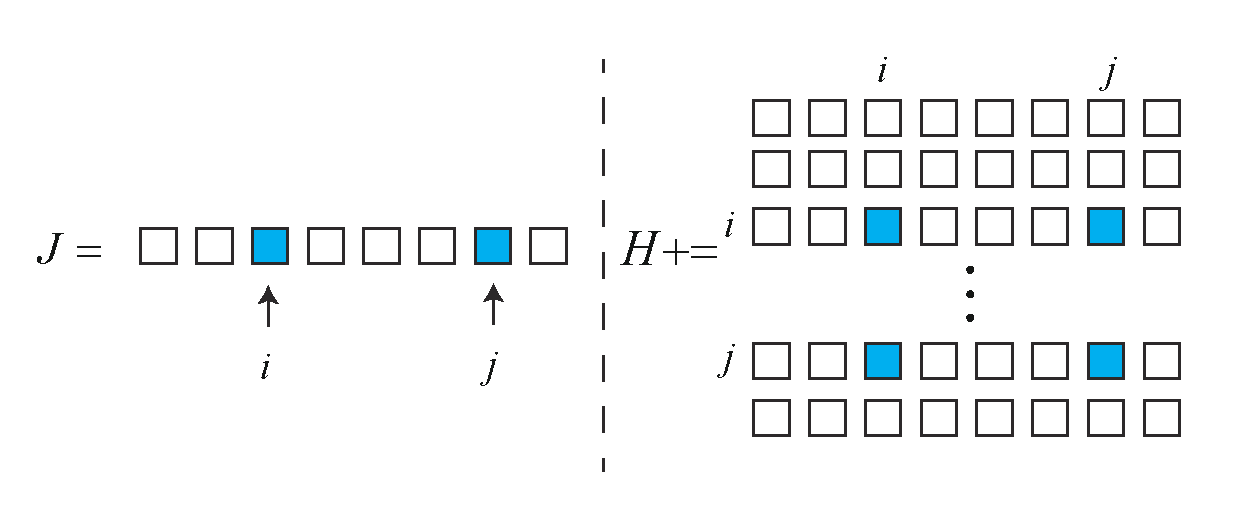
\includegraphics[width=0.3\linewidth]{vo1/sparse}
%    \includegraphics[width=0.3\linewidth]{vo1/semidense}
%    \includegraphics[width=0.3\linewidth]{vo1/dense}
%    \caption{Sparse map, semi-dense map and dense map}
%    \label{fig:threemethods}
%\end{figure}
% !Mode:: "TeX:UTF-8"
\chapter{Visual Odometry: Part 2}
\label{cpt:vo2}
\begin{mdframed}  
	\textbf{Goal of Study}
	\begin{enumerate}[labelindent=0em,leftmargin=1.5em]
		\item Understand the principle of optical flow to track feature points.
		\item Understand how the direct method estimates the camera pose.
		\item Use g2o for direct method.
	\end{enumerate}
\end{mdframed}

Different from feature point method, direct method is another main stream of visual odometry. Despite that it has not yet become the mainstream of VO, after recent years of development, the direct method can compete with feature point method to some extent. In this chapter, we will introduce the principle of the direct method and implement its core part.

\newpage
\includepdf{resources/other/ch8.pdf}

\newpage
\section{Origin of the direct method}
In the last chapter, we introduced using feature points to estimate camera motion. Although the feature point method plays a key role in visual odometry, researchers still believe that it has at least the following shortcomings:

\begin{enumerate}
	\item The extraction of key points and the calculation of descriptors are very time-consuming. In practice, SIFT currently cannot be calculated in real time on the CPU, and ORB also requires nearly 20ms of calculation. If the entire SLAM runs at a speed of 30 milliseconds per frame, more than half of the time will be spent on feature points calculation.

	\item When using feature points, all information except feature points is ignored. An image has hundreds of thousands of pixels, but only a few hundred feature points. Using only feature points discards most of the \textbf{possibly useful} image information. 
	
	\item The camera sometimes moves to places \textbf{lack of feature}, where there is often no obvious texture information. For example, sometimes we will face a white wall or an empty corridor. The number of feature points in these scenes will be significantly reduced, and we may not find enough matching points to calculate camera motion.。
\end{enumerate}

Now we see that there are indeed some problems with using feature points. Is there any way to overcome these shortcomings? We have the following ideas:

\begin{itemize}
	\item Keep feature points, but discard their descriptors. At the same time, use \textbf{Optical Flow} to track the motion of feature points. This can avoid the time brought by the calculation and matching of the descriptor, and the time spent on calculating optical flow itself is less than the descriptor calculation and matching.
	\item Only calculate key points, not descriptors. At the same time, use \textbf{Direct Method} to calculate the position of the feature point in the image at the next timestamp. This can also save the time spent on the calculation of the descriptor as well as the the calculation of optical flow.	
\end{itemize}

The first method still uses feature points, but substitutes the descriptor matching with optical flow tracking, and still uses epipolar geometry, PnP or ICP algorithms to estimate camera motion. This still requires that the extracted keypoints are distinguishable, that is, we need to extract the corner points. In the direct method, we will estimate the camera motion and the projection of the points at the same time according to the \textbf{pixel gray information} of the image, and the extracted points to be corner points is not longer a hard prerequisite. As you will see later, they can even be randomly selected points.

When using the feature point method to estimate camera motion, we regard feature points as fixed points in three-dimensional space. According to their projection position in the camera, the camera motion is optimized by \textbf{minimize reprojection error}. In this process, we need to know exactly the pixel position of the spatial point after the projection of the two cameras-this is why we need to match or track the features. Meanwhile, computing and matching features requires a lot of computation. In contrast, in the direct method, we do not need to know the correspondence between points in advance, but find it by minimizing \textbf{Photometric error}.

We will focus on the direct method in this chapter. It is to overcome the shortcomings of the feature point method listed above. The direct method estimates the camera motion based on the brightness information of the pixels, and can completely eliminate the calculation of keypoints and descriptors. Therefore, it not only saves the calculation time of features, but also solves the problems caused by lacking features. As long as there are brightness changes in the scene (it can be a gradual change without forming a local image gradient), the direct method will work. According to the number of pixels used, the direct method can be categorized into sparse, semi-dense and dense. Compared with the feature point method that can only reconstruct sparse feature points (sparse map), the direct method also has the capability to restore semi-dense or dense structures.

Historically, there were also early uses of the direct method \textsuperscript{\cite{Silveira2008}}. With the emergence of some open source projects that use the direct method, such as SVO\textsuperscript{\cite{Forster2014}}, LSD-SLAM\textsuperscript{\cite{Engel2014}}, DSO\textsuperscript{\cite{Engel2016}}, etc. Direct method became a more and more important part of the visual odometry.

\section{2D Optical Flow}
Direct method was inspired by the optical flow. They are similar and use the same assumptions. Optical flow describes the motion of pixels in the image, and the direct method is accompanied by a camera motion model. Before the direct method, we will introduce optical flow first.

Optical flow is a method of describing the movement of pixels between images, as shown in \autoref{fig:LK}~. The same pixel will move in the image over time, and we want to track its movement. The calculation of motion of a portion of pixels is called \textbf{sparse optical flow}, and the calculation of all pixels in an image is called \textbf{dense optical flow}. A well-known sparse optical flow method is called Lucas-Kanade optical flow \textsuperscript{\cite{Lucas1981}}. It can be used to track the position of feature points in SLAM. Dense optical flow is represented by Horn-Schunck optical flow \textsuperscript{\cite{Horn1981}}. This section mainly introduces Lucas-Kanade optical flow, also known as LK optical flow.

\begin{figure}[!htp]
	\centering
	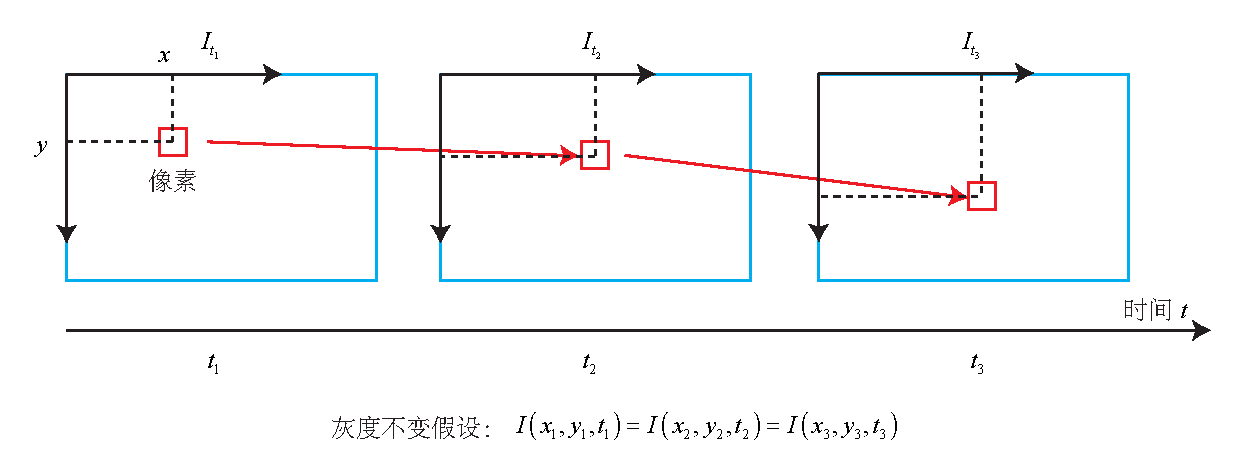
\includegraphics[width=1.0\linewidth]{vo2/opticalFlow}
	\caption{workflow of LK method}
	\label{fig:LK}
\end{figure}

\subsection*{Lucas-Kanade optical flow}
In the LK optical flow, we think that the image from the camera changes over time. The image can be regarded as a function of time $\mathbf{I}(t)$. Then, for a pixel at $(x,y)$ at time $t$, its grayscale can be written as
\[
\mathbf{I}(x,y,t).
\]
In this way, the image is regarded as a function of position and time, and its range is the grayscale of the pixels in the image. Now consider a fixed point in space, its pixel coordinates at time $t$ are $x,y$. Due to the movement of the camera, its image coordinates will change. We want to estimate the position of this space point in the image at other times. How to estimate it? Here we will introduce the basic assumptions of the optical flow method.

\textbf{Constant Brightness}:The pixel grayvalue of the same space point is constant in each image.

For the pixel at $(x,y)$ at time $t$, suppose it moves to $(x+\mathrm{d}x, y+\mathrm{d}y)$ at time $t+\mathrm{d}t$. Since the grayscale is unchanged, we have:
\begin{equation} 
\mathbf{I}(x+\mathrm{d}x, y+\mathrm{d}y, t+\mathrm{d}t) = \mathbf{I} (x,y,t).
\end{equation}

Note that in the most of time in practice the assumption of constant brightness is not true. In fact, due to the different materials of the objects, the pixels will have highlights and shadows; sometimes, the camera will automatically adjust its exposure parameters to make the overall image brighter or darker. At these times, the assumption of constant brightness is invalid, so the result of optical flow is not necessarily reliable. However, on the other hand, all algorithms work under certain assumptions. If we do not make any assumptions, we cannot design practical algorithms. So, let us consider this assumption to be true for now and see how to calculate the motion of the pixels.

Carry out Taylor expansion on the left side and only keep the first-order term, we have:
\begin{equation}
\mathbf{I} \left( {x + \mathrm{d}x,y + \mathrm{d}y,t + \mathrm{d}t} \right) \approx \mathbf{I} \left( {x,y,t} \right) + \frac{{\partial \mathbf{I} }}{{\partial x}}\mathrm{d}x + \frac{{\partial \mathbf{I}}}{{\partial y}}\mathrm{d}y + \frac{{\partial \mathbf{I}}}{{\partial t}}\mathrm{d}t.
\end{equation}

Because we assume that the brightness does not change, the brightness at the next timestamp is equal to the current one, thus:
\begin{equation}
 \frac{{\partial \mathbf{I} }}{{\partial x}}\mathrm{d}x + \frac{{\partial \mathbf{I}}}{{\partial y}}\mathrm{d}y + \frac{{\partial \mathbf{I}}}{{\partial t}}\mathrm{d}t = 0.
\end{equation}

Divide both sides by $\mathrm{d}t$:
\begin{equation}\label{key}
 \frac{{\partial \mathbf{I} }}{{\partial x}} \frac{\mathrm{d}x}{\mathrm{d}t} + \frac{{\partial \mathbf{I}}}{{\partial y}} \frac{\mathrm{d}y}{\mathrm{d}t} =- \frac{{\partial \mathbf{I}}}{{\partial t}}.
\end{equation}

Where $\mathrm{d}x / \mathrm{d}t$ is the speed of the pixel on the $x$ axis, and $\mathrm{d}y/\mathrm{d}t$ is the speed on the $y$ axis, denoting them as $u,v$. At the same time, $\partial \mathbf{I}/{\partial x}$ is the gradient of the image in the $x$ direction at this point, and the other is the gradient in the $y$ direction, denoted as $\mathbf{I} _x, \mathbf{I}_y$. Denote the change of the image brightness with respect to time as $\mathbf{I}_t$. They can be written in a matrix form as:
\begin{equation}
\left[ {\begin{array}{*{20}{c}}
	{{ \mathbf{I}_x}}&{{ \mathbf{I}_y}}
	\end{array}} \right]\left[ \begin{array}{l}
u\\
v
\end{array} \right] =  - {\mathbf{I}_t}.
\end{equation}

What we want is to calculate the motion $u,v$ of the pixel, but this formula is a linear equation with two variables, and we cannot find $u,v$ by itself. Therefore, additional constraints are needed to calculate $u,v$. In LK optical flow, we assume \textbf{pixels in a certain window have the same motion}.

Consider a window of size $w \times w$, which contains $w^2$ pixels. Since the pixels in this window are assumed to have the same motion, we have a total of $w^2$ equations:
\begin{equation}
\left[ {\begin{array}{*{20}{c}}
	{{ \mathbf{I}_x}}&{{ \mathbf{I}_y}}
	\end{array}} \right]_k
\left[ \begin{array}{l}
u\\
v
\end{array} \right] =  - {\mathbf{I}_t}_k, \quad k=1, \ldots, w^2.
\end{equation}

Stacking them:
\begin{equation}
\mathbf{A} = \left[ {\begin{array}{*{20}{c}}
	{{{\left[ {{\mathbf{I}_x},{\mathbf{I}_y}} \right]}_1}}\\
	\vdots \\
	{{{\left[ {{\mathbf{I}_x},{\mathbf{I}_y}} \right]}_k}}
	\end{array}} \right],\mathbf{b} = \left[ {\begin{array}{*{20}{c}}
	{{ \mathbf{I}_{t1}}}\\
	\vdots \\
	{{ \mathbf{I}_{tk}}}
	\end{array}} \right].
\end{equation}

The whole equation is:
\begin{equation}
\mathbf{A}\left[ \begin{array}{l}
u\\
v
\end{array} \right] =  - \mathbf{b}.
\end{equation}

This is an overdetermined linear equation about $u,v$. And we can find its least square solution.
\begin{equation}
{\left[ \begin{array}{l}
	u\\
	v
	\end{array} \right]^*} = -{\left( {{ \mathbf{A}^\mathrm{T}}\mathbf{A}} \right)^{ - 1}}{ \mathbf{A}^\mathrm{T}}\mathbf{b}.
\end{equation}

In this way, the speed $u,v$ of pixels between images is obtained. When $t$ takes discrete moments instead of continuous time, we can estimate the position of a block of pixels in several images. Since the pixel gradient is only valid locally, if one iteration does not produce a reasonable result, we will iterate this calculation several times. In SLAM, LK optical flow is often used to track the motion of corner points. We can have a deeper understanding of it through the program.

\section{Practice: LK Optical Flow}
\label{sec:LKFlow}
%\subsection{Use TUM Dataset online}
%The following demonstrates how to use the optical flow method provided by OpenCV to track feature points. As in the previous section, we have prepared several dataset images, which are stored in the data/ folder. They come from the public RGB-D dataset (TUM dataset) \footnote{see \url{http://vision.in.tum.de/data/datasets/rgbd-dataset/download} provided by the Technical University of Munich}. It contains many RGB-D videos, which can be used as experimental data for RGB-D or monocular SLAM. It also provides an accurate trajectory measured by the motion capture system, which can be used as a standard trajectory to calibrate the SLAM system. Because the data set is relatively large, we did not put it on GitHub, please go to the dataset homepage to retrieve the corresponding data. Part of the images in the "freburg1\_desk" data set are used in this program. Readers can find its download link on the TUM dataset homepage. Or, you can directly use the part of it provided on GitHub repo.
%
%Our data is located under data/ in the directory of this chapter as a compressed package (data.tar.gz). Since the TUM data set is collected from the actual environment, it is necessary to explain its data format (data sets generally have their own defined format). After unzipping, you will see the following files:
%
%\begin{enumerate}
% 	\item rgb.txt and depth.txt record the collection time of each file and the corresponding file name.
% 	\item rgb/ and depth/ directories store the captured PNG format image files. The color image is 8-bit 3 channels, and the depth map is 16-bit single-channel image. The file name is the collection time.
%	
% 	\item groundtruth.txt is the camera pose collected by the external motion capture system, the format is
% 	\[
% 	(\mathrm{time}, t_x, t_y, t_z, q_x, q_y, q_z, q_w),
% 	\]
% 	We can treat it as a standard trajectory (ground truth).
%\end{enumerate}
%
%Please note that the collection of color image, depth image and standard trajectory are all independent, and the trajectory collection frequency is much higher than that of the image. Before using the data, it is necessary to align the data in time according to the collection time in order to pair the color map and the depth map. In principle, we can regard data whose collection time is close to a threshold as a pair of images. And regard the pose at a similar time as the true collection position of the image. TUM provides a Python script "associate.py" (or use slambook/tools/associate.py) to help us accomplish this. Please put this file in the data set directory and run:
%\begin{lstlisting}[language=sh]
%python associate.py rgb.txt depth.txt> associate.txt
%\end{lstlisting}
%
%This script will match according to the collection time in the two input files, and finally output to the file associate.txt. The output file contains the time and file name information of the two images after pairing, which can be used as the source for subsequent processing. In addition, the TUM data set also provides tools for comparing estimated trajectories with standard trajectories. We will introduce them when they are used.
\subsection{Use LK optical flow}
In the practice, we will use several sample images to track their feature points with OpenCV optical flow. At the same time, we will also manually implement a LK optical flow for a comprehensive understanding. We use two sample images from the Euroc dataset, extract the corner points in the first image, and then use optical flow to track their position in the second image. First, let's use the LK optical flow in OpenCV:

\begin{lstlisting}[language=c++,caption=slambook2/ch8/optical_flow.cpp (snippet))]
// use opencv's flow for validation
vector<Point2f> pt1, pt2;
for (auto &kp: kp1) pt1.push_back(kp.pt);
vector<uchar> status;
vector<float> error;
cv::calcOpticalFlowPyrLK(img1, img2, pt1, pt2, status, error);
\end{lstlisting}

The optical flow in OpenCV is very simple to use. You only need to call the cv::calcOpticalFlowPyrLK function, provide two images and the corresponding feature points, you can get the tracked points, as well as the status and error of each point. We can determine whether the corresponding point is tracked correctly according to whether the status variable is 1. This function also has some optional parameters, but in the demonstration we only use the default parameters. We omit other codes that mention features and draw results here, which have been shown in the previous code snippet.

\subsection{Implement optical flow with Gauss Newton method}
\subsubsection{Single-layer optical flow}
Optical flow can also be seen as an optimization problem: by minimizing the grayscale error, the optimal pixel shift is estimated. Therefore, similar to those various Gauss-Newton methods previously implemented, we now also implement an optical flow based on the Gauss-Newton method.

\begin{lstlisting}[language=c++,caption=slambook2/ch8/optical_flow.cpp (snippet))]
class OpticalFlowTracker {
public:
	OpticalFlowTracker(
		const Mat &img1_,
		const Mat &img2_,
		const vector<KeyPoint> &kp1_,
		vector<KeyPoint> &kp2_,
		vector<bool> &success_,
		bool inverse_ = true, bool has_initial_ = false) :
		img1(img1_), img2(img2_), kp1(kp1_), kp2(kp2_), success(success_), inverse(inverse_),
		has_initial(has_initial_) {}
	
	void calculateOpticalFlow(const Range &range);

private:
	const Mat &img1;
	const Mat &img2;
	const vector<KeyPoint> &kp1;
	vector<KeyPoint> &kp2;
	vector<bool> &success;
	bool inverse = true;
	bool has_initial = false;
};

void OpticalFlowSingleLevel(
	const Mat &img1,
	const Mat &img2,
	const vector<KeyPoint> &kp1,
	vector<KeyPoint> &kp2,
	vector<bool> &success,
	bool inverse, bool has_initial) {
	kp2.resize(kp1.size());
	success.resize(kp1.size());
	OpticalFlowTracker tracker(img1, img2, kp1, kp2, success, inverse, has_initial);
	parallel_for_(Range(0, kp1.size()),
		std::bind(&OpticalFlowTracker::calculateOpticalFlow, &tracker, placeholders::_1));
}

void OpticalFlowTracker::calculateOpticalFlow(const Range &range) {
	// parameters
	int half_patch_size = 4;
	int iterations = 10;
	for (size_t i = range.start; i < range.end; i++) {
		auto kp = kp1[i];
		double dx = 0, dy = 0; // dx,dy need to be estimated
		if (has_initial) {
			dx = kp2[i].pt.x - kp.pt.x;
			dy = kp2[i].pt.y - kp.pt.y;
		}
		
		double cost = 0, lastCost = 0;
		bool succ = true; // indicate if this point succeeded
		
		// Gauss-Newton iterations
		Eigen::Matrix2d H = Eigen::Matrix2d::Zero();    // hessian
		Eigen::Vector2d b = Eigen::Vector2d::Zero();    // bias
		Eigen::Vector2d J;  // jacobian
		for (int iter = 0; iter < iterations; iter++) {
			if (inverse == false) {
				H = Eigen::Matrix2d::Zero();
				b = Eigen::Vector2d::Zero();
			} else {
				// only reset b
				b = Eigen::Vector2d::Zero();
			}
			
			cost = 0;
			
			// compute cost and jacobian
			for (int x = -half_patch_size; x < half_patch_size; x++)
			for (int y = -half_patch_size; y < half_patch_size; y++) {
				double error = GetPixelValue(img1, kp.pt.x + x, kp.pt.y + y) -
					GetPixelValue(img2, kp.pt.x + x + dx, kp.pt.y + y + dy);;  // Jacobian
				if (inverse == false) {
					J = -1.0 * Eigen::Vector2d(
						0.5 * (GetPixelValue(img2, kp.pt.x + dx + x + 1, kp.pt.y + dy + y) -
							GetPixelValue(img2, kp.pt.x + dx + x - 1, kp.pt.y + dy + y)),
						0.5 * (GetPixelValue(img2, kp.pt.x + dx + x, kp.pt.y + dy + y + 1) -
							GetPixelValue(img2, kp.pt.x + dx + x, kp.pt.y + dy + y - 1))
					);
				} else if (iter == 0) {
					// in inverse mode, J keeps same for all iterations
					// NOTE this J does not change when dx, dy is updated, so we can store it and only compute error
					J = -1.0 * Eigen::Vector2d(
						0.5 * (GetPixelValue(img1, kp.pt.x + x + 1, kp.pt.y + y) -
							GetPixelValue(img1, kp.pt.x + x - 1, kp.pt.y + y)),
						0.5 * (GetPixelValue(img1, kp.pt.x + x, kp.pt.y + y + 1) -
							GetPixelValue(img1, kp.pt.x + x, kp.pt.y + y - 1))
					);
				}
				// compute H, b and set cost;
				b += -error * J;
				cost += error * error;
				if (inverse == false || iter == 0) {
					// also update H
					H += J * J.transpose();
				}
			}
			
			// compute update
			Eigen::Vector2d update = H.ldlt().solve(b);
			
			if (std::isnan(update[0])) {
				// sometimes occurred when we have a black or white patch and H is irreversible
				cout << "update is nan" << endl;
				succ = false;
				break;
			}
			
			if (iter > 0 && cost > lastCost) {
				break;
			}
			
			// update dx, dy
			dx += update[0];
			dy += update[1];
			lastCost = cost;
			succ = true;
			
			if (update.norm() < 1e-2) {
				// converge
				break;
			}
		}
		
		success[i] = succ;
		
		// set kp2
		kp2[i].pt = kp.pt + Point2f(dx, dy);
	}
}
\end{lstlisting}

We have implemented a single-layer optical flow function in the OpticalFlowSingleLevel function, in which cv::parallel\_for\_ is called in parallel to call OpticalFlowTracker::calculateOpticalFlow, which calculates the optical flow of feature points within a specified range. This parallel for loop is internally implemented by the Intel tbb library. We only need to define the function body according to its interface, and then pass the function to it as a std::function object.

In the implementation of calculateOpticalFlow, we solve such a problem:
\begin{equation}
\mathop {\min }\limits_{\Delta x,\Delta y} \left\| {{\mathbf{I}_1}\left( {x,y} \right) - {\mathbf{I}_2}\left( {x + \Delta x,y + \Delta y} \right)} \right\|_2^2.
\end{equation}
Therefore, the residual is the part inside the brackets, and the corresponding Jacobian is the gradient of the second image at $x + \Delta x,y + \Delta y$. In addition, according to \cite{Baker2004}, the gradient can also be replaced by the gradient $\mathbf{I}_1 (x,y)$ of the first image. This is called \textbf{Inverse} optical flow method. In inverse optical flow, the gradient of $\mathbf{I}_1 (x,y)$ remains unchanged, so we can use the result calculated in the first iteration in the subsequent iterations. When the Jacobian remains unchanged, the $\mathbf{H}$ matrix is unchanged, and only the residual is calculated for each iteration, which can save a lot of calculation.

\subsubsection{Multi-layer optical flow}
Since we write optical flow as an optimization problem, we must assume that the initial value of optimization is close to the optimal value to ensure the convergence of the algorithm. Therefore, if the camera moves faster and the difference between the two images is obvious, the single-layer image optical flow method can be easily stuck at a local minimum. While it can be resolved to some extent by image pyramids.

\begin{figure}[!htp]
	\centering
	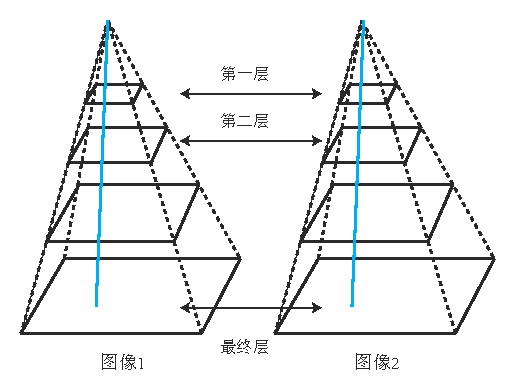
\includegraphics[width=.7\linewidth]{vo2/image-pyramid}
	\caption{Image pyramid and coarse-to-fine process.}
	\label{fig:image-pyramid}
\end{figure}

Image pyramid refers to scaling the image to get samples in different resolutions, as shown in \autoref{fig:image-pyramid}. The original image is used as the bottom layer of the pyramid. Every time one layer goes up, the lower layer image is scaled to a certain magnification, and then a pyramid is obtained. When calculating the optical flow, start from the top layer image, and then use the tracking result of the previous layer as the initial value of the optical flow of the next layer. Since the upper layer image is relatively rough, this process is also called \textbf{coarse-to-fine} optical flow, which is also the usual process of optical flow in practice.

The advantage of going from coarse to fine is that when the pixel motion of the original image is large, the motion is still within a small range from the image at the top of the pyramid. For example, if the feature points of the original image move by 20 pixels, it is easy for the optimization to be trapped in the minimum value due to the non-convexity of the image. But now suppose there is a pyramid with a zoom magnification of 0.5 times, then in the upper two layers of images, the pixel movement is only 5 pixels, and the result is obviously better than directly optimizing on the original image.

We have implemented multi-layer optical flow in the program, the code is as follows:
\begin{lstlisting}[language=c++,caption=slambook2/ch8/optical_flow.cpp (snippet)]
void OpticalFlowMultiLevel(
	const Mat &img1,
	const Mat &img2,
	const vector<KeyPoint> &kp1,
	vector<KeyPoint> &kp2,
	vector<bool> &success,
	bool inverse) {
	
	// parameters
	int pyramids = 4;
	double pyramid_scale = 0.5;
	double scales[] = {1.0, 0.5, 0.25, 0.125};
	
	// create pyramids
	vector<Mat> pyr1, pyr2; // image pyramids
	for (int i = 0; i < pyramids; i++) {
		if (i == 0) {
			pyr1.push_back(img1);
			pyr2.push_back(img2);
		} else {
			Mat img1_pyr, img2_pyr;
			cv::resize(pyr1[i - 1], img1_pyr,
			cv::Size(pyr1[i - 1].cols * pyramid_scale, pyr1[i - 1].rows * pyramid_scale));
			cv::resize(pyr2[i - 1], img2_pyr,
			cv::Size(pyr2[i - 1].cols * pyramid_scale, pyr2[i - 1].rows * pyramid_scale));
			pyr1.push_back(img1_pyr);
			pyr2.push_back(img2_pyr);
		}
	}

	// coarse-to-fine LK tracking in pyramids
	vector<KeyPoint> kp1_pyr, kp2_pyr;
	for (auto &kp:kp1) {
		auto kp_top = kp;
		kp_top.pt *= scales[pyramids - 1];
		kp1_pyr.push_back(kp_top);
		kp2_pyr.push_back(kp_top);
	}
	
	for (int level = pyramids - 1; level >= 0; level--) {
		// from coarse to fine
		success.clear();
		OpticalFlowSingleLevel(pyr1[level], pyr2[level], kp1_pyr, kp2_pyr, success, inverse, true);
		
		if (level > 0) {
			for (auto &kp: kp1_pyr)
			kp.pt /= pyramid_scale;
			for (auto &kp: kp2_pyr)
			kp.pt /= pyramid_scale;
		}
	}
	
	for (auto &kp: kp2_pyr)
		kp2.push_back(kp);
}
\end{lstlisting}

This code constructs a four-layer pyramid with a scaling rate of 0.5, and calls the single-layer optical flow function to achieve the multi-layer optical flow. In the main function, we tested the performance of OpenCV's optical flow, single-layer optical flow, and multi-layer optical flow on two images, and recorded their runtime:
\begin{lstlisting}[language=sh,caption=终端输入:]
./build/optical_flow
build pyramid time: 0.000150349
track pyr 3 cost time: 0.000304633
track pyr 2 cost time: 0.000392889
track pyr 1 cost time: 0.000382347
track pyr 0 cost time: 0.000375099
optical flow by gauss-newton: 0.00189268
optical flow by opencv: 0.00220134
\end{lstlisting}
In terms of runtime, the multi-layer optical flow method takes roughly the same time as OpenCV. Since the performance of the parallelized program varies from run to run, these numbers will not be exactly the same on the reader's machine. For the result of optical flow, see \autoref{fig:optical-flow-result}. It can be seen that the multi-layer optical flow has the same effect as OpenCV, and the single-layer optical flow performs obviously worser than the multi-layer optical flow.

\begin{figure}[!htp]
	\centering
	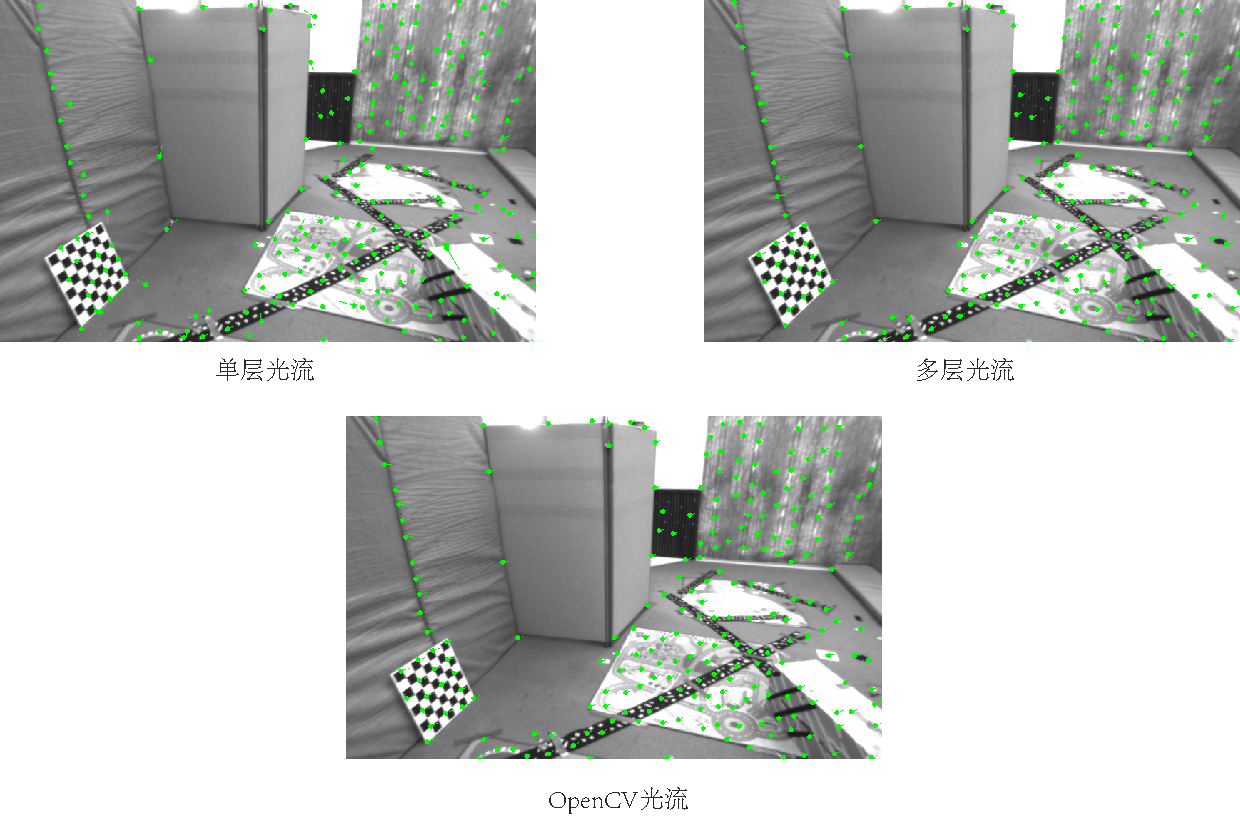
\includegraphics[width=.85\linewidth]{vo2/optical-flow}
	\caption{Comparison of the results of various optical flows}
	\label{fig:optical-flow-result}
\end{figure}

\subsection{Summary of optical flow practice}
We see that LK optical flow can directly obtain the corresponding relationship of feature points. This correspondence is like the matching of descriptors, except that optical flow requires higher image continuity and light stability. We can use PnP, ICP, or epipolar geometry to estimate the camera motion through the feature points tracked by optical flow. These methods were introduced in the previous lecture and will not be discussed here.

In terms of runtime, it extracts about 230 feature points in the experiment. OpenCV and multi-layer optical flow need about 2 milliseconds to complete the tracking (the CPU I use is Intel I7-8550U), which is quite fast. If we use keypoints like FAST, then the entire optical flow calculation can be done in about 5 milliseconds, which is very fast compared to feature matching. However, if the position of the corner point is not good, the optical flow is also easy to be lost or give wrong results, which requires the subsequent algorithm to have a certain outlier removal mechanism, we leave the relevant discussion to the later chapter.

In a nutshell, the optical flow method can accelerate the visual odometry calculation method based on feature points by avoiding the process of calculating and matching descriptors, but requires smoother camera movement (or higher collection frequency).

\section{Direct Method}
Next, let's discuss the direct method, which is somehow similar to the optical flow method. We first introduce the principle of the direct method, and then implement the direct method.

\subsection{Derivation of the direct method}
In the optical flow, we will first track the location of feature points, and then determine the camera's movement based on these locations. Then, such a two-step plan is difficult to guarantee the overall optimality. We can ask, can we adjust the result of the previous step in the latter step? For example, if I think that the camera has turned 15 degrees to the right, can the optical flow use this 15-degree motion as the initial value to adjust the calculation of the optical flow? This idea is reflected in the direct method.

As shown in \autoref{fig:directMethod}~, consider a spatial point $P$ and camera at two timestamps. The world coordinates of $P$ are $[X,Y,Z]$, and the pixel coordinates of its imaging on two cameras are $\mathbf{p}_1, \mathbf{p}_2$.

\begin{figure}[!htp]
	\centering
	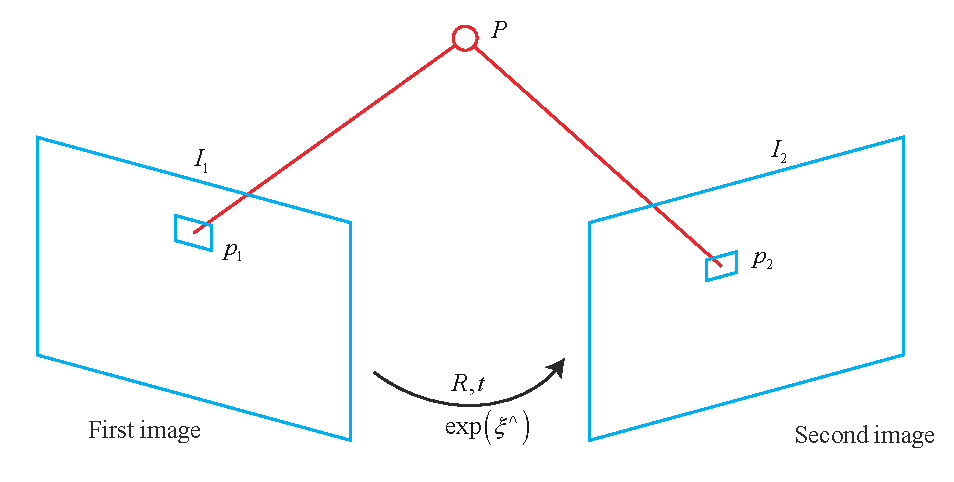
\includegraphics[width=.85\linewidth]{vo2/directMethod}
	\caption{the direct method.}
	\label{fig:directMethod}
\end{figure}

Our goal is to find the relative pose transformation from the first camera to the second camera. We take the first camera as the frame of reference, and set the rotation and translation of the second camera as $\mathbf{R}, \mathbf{t}$ (corresponding to the Lie group as $\mathbf{T}$). At the same time, the internal parameters of the two cameras are the same, denoted as $\mathbf{K}$. Let's write down the complete projection equation:
\begin{align*}
{\mathbf{p}_1} &= {\left[ \begin{array}{l}
	u\\
	v\\
	1
	\end{array} \right]_1} = \frac{1}{Z_1} \mathbf{KP}, \\
{\mathbf{p}_2} &= {\left[ \begin{array}{l}
	u\\
	v\\
	1
	\end{array} \right]_2} = \frac{1}{Z_2} \mathbf{K}\left( {\mathbf{RP} +\mathbf{t}} \right) = \frac{1}{Z_2} \mathbf{K} \left(\mathbf{T}  \mathbf{P} \right)_{1:3}.
\end{align*}
Where $Z_1$ is the depth of $P$, and $Z_2$ is the depth of $P$ in the second camera frame, which is the third coordinate of $\mathbf{RP}+\mathbf{t}$ . Since $\mathbf{T}$ can only be multiplied with homogeneous coordinates, we need to take out the first 3 elements after multiplying. This is consistent with the content of \ref{cpt:5}.

Recall that in the feature point method, since we know the pixel positions of $\mathbf{p}_1, \mathbf{p}_2$ through matching descriptors, we can calculate the reprojection position. But in the direct method, since there is no feature matching, we have no way of knowing which $\mathbf{p}_2$ and $\mathbf{p}_1$ correspond to the same point. The idea of the direct method is to find the position of $\mathbf{p}_2$ according to the current camera pose estimation. But if the camera pose is not good enough, the appearance of $\mathbf{p}_2$ and $\mathbf{p}_1$ will be significantly different. Therefore, in order to reduce this difference, we optimize the pose of the camera to find $\mathbf{p}_2$ that is more similar to $\mathbf{p}_1$. This can also be done by solving an optimization problem, but at this time it is not to minimize the reprojection error, but to minimize the \textbf{Photometric Error}, which is the brightness error of the two pixels of $P$:
\begin{equation}
e = {\mathbf{I}_1}\left( {{\mathbf{p}_1}} \right) - {\mathbf{I}_2}\left( {{\mathbf{p}_2}} \right).
\end{equation}

Note that $e$ is a scalar here. Similarly, the optimization is with respect to the second norm of the error, taking the unweighted form for now, as:
\begin{equation}
\mathop {\min }\limits_{\mathbf{T}}  J\left( \mathbf{T}  \right) = \|e\|^2.
\end{equation}

The optimization is based on \textbf{constant brightness assumption}. We assume that the grayscale of a spatial point imaged at various viewing points is constant. If we have many (for example, $N$) space points $P_i$, then the whole camera pose estimation problem becomes
\begin{equation}
\mathop {\min }\limits_{\mathbf{T}}  J\left( \mathbf{T}  \right) = \sum\limits_{i = 1}^N {e_i^\mathrm{T}{e_i}}, \quad {e_i} = {\mathbf{I}_1}\left( {{\mathbf{p}_{1,i}}} \right) - {\mathbf{I}_2}\left( {{ \mathbf{p}_{2,i}}} \right).
\end{equation}

The variable to be optimized here is the camera pose $\mathbf{T}$, instead of the motion of each feature point in the optical flow. In order to solve this optimization problem, we are concerned about how the error $e$ changes with the camera pose $\mathbf{T}$, and we need to analyze their derivative relationship. First, define two intermediate variables:
\begin{align*}
\mathbf{q} &= \mathbf{T} \mathbf{P}, \\
\mathbf{u} &= \frac{1}{{{Z_2}}} \mathbf{K} \mathbf{q}.
\end{align*}
Here, $\mathbf{q}$ is the coordinates of $P$ in the second camera coordinate system, and $\mathbf{u}$ is its pixel coordinates. Obviously $\mathbf{q}$ is a function of $\mathbf{T}$, and $\mathbf{u}$ is a function of $\mathbf{q}$, and thus is also a function of $\mathbf{T}$. Consider the left perturbation model of Lie algebra, using the first-order Taylor expansion:
\begin{equation}
e(\mathbf{T})=\mathbf{I}_1(\mathbf{p}_{1})-\mathbf{I}_2(\mathbf{u}),
\end{equation}
所以:
\begin{equation}
\frac{\partial e}{\partial \mathbf{T}} = \frac{{\partial {\mathbf{I}_2}}}{{\partial \mathbf{u}}}\frac{{\partial \mathbf{u}}}{{\partial \mathbf{q}}}\frac{{\partial \mathbf{q}}}{{\partial \delta \mathbf{\xi} }}\delta \mathbf{\xi},
\end{equation}
Where $\delta \mathbf{\xi}$ is the left disturbance of $\mathbf{T}$. We see that the first derivative is divided into 3 terms due to the chain rule, and these 3 terms are easy to obtain:

\begin{enumerate}
	\item $ \partial \mathbf{I}_2 / \partial \mathbf{u} $ is the grayscale gradient at pixel $\mathbf{u}$.
	\item $ \partial \mathbf{u} / \partial \mathbf{q} $ is the derivative of the projection equation with respect to the three-dimensional point in the camera frame. Remember $\mathbf{q}=[X,Y,Z]^\mathrm{T}$, according to $\ref{cpt:7}$, the derivative is
	\begin{equation}
	\frac{{\partial \mathbf{u}}}{{\partial \mathbf{q}}} = \left[ {\begin{array}{*{20}{c}}
		{\frac{{\partial u}}{{\partial X}}}&{\frac{{\partial u}}{{\partial Y}}}&{\frac{{\partial u}}{{\partial Z}}}\\
		{\frac{{\partial v}}{{\partial X}}}&{\frac{{\partial v}}{{\partial Y}}}&{\frac{{\partial v}}{{\partial Z}}}
		\end{array}} \right] = \left[ {\begin{array}{*{20}{c}}
		{\frac{{{f_x}}}{{\rm{Z}}}}&0&{ - \frac{{{f_x}X}}{{{Z^2}}}}\\
		0&{\frac{{{f_y}}}{Z}}&{ - \frac{{{f_y}Y}}{{{Z^2}}}}
		\end{array}} \right].
	\end{equation}
	
	\item ${\partial \mathbf{q}}/{\partial \delta \mathbf{\xi} }$is the derivative of the transformed three-dimensional point with respect to the transformation, which was introduced in the chapter of Lie Algebra:
	\begin{equation}
	\frac{{\partial \mathbf{q}}}{{\partial \delta \mathbf{\xi} }} = \left[ { \mathbf{I}, - {\mathbf{q}^ \wedge }} \right].
	\end{equation}
\end{enumerate}

In practice, the last two items are only related to the three-dimensional point $\mathbf{q}$ irrelevant to the image, we often combine them together:
\begin{equation}
\frac{{\partial \mathbf{u}}}{{\partial \delta \mathbf{\xi} }} = \left[ {\begin{array}{*{20}{c}}
	{\frac{{{f_x}}}{Z}}&0&{ - \frac{{{f_x}X}}{{{Z^2}}}}&{ - \frac{{{f_x}XY}}{{{Z^2}}}}&{{f_x} + \frac{{{f_x}{X^2}}}{{{Z^2}}}}&{ - \frac{{{f_x}Y}}{Z}}\\
	0&{\frac{{{f_y}}}{Z}}&{ - \frac{{{f_y}Y}}{{{Z^2}}}}&{ - {f_y} - \frac{{{f_y}{Y^2}}}{{{Z^2}}}}&{\frac{{{f_y}XY}}{{{Z^2}}}}&{\frac{{{f_y}X}}{Z}}
	\end{array}} \right].
\end{equation}

This $2 \times 6$ matrix also appeared in the last chapter. Therefore, we derive the Jacobian of residual with respect to Lie algebra:
\begin{equation}
\label{eq:jacobianofDirect}
\mathbf{J} =  - \frac{{\partial { \mathbf{I}_2}}}{{\partial \mathbf{u}}}\frac{{\partial \mathbf{u}}}{{\partial \delta \mathbf{\xi} }}.
\end{equation}

For the problem of $N$ points, we can use this method to calculate the Jacobian of the optimization problem, and then use the Gauss Newton method or Levenberg-Marquardt method to calculate the increments and iteratively solve it. So far, we have introduced the entire process of the direct method to estimate the camera pose. Let's implement the direct method in a program.

\subsection{Discussion of Direct Method}
In the above derivation, $P$ is a spatial point with a known location. How did it come from? Under the RGB-D camera, we can reproject any pixel into the three-dimensional space, and then project it into the next image. If it is binocular, the pixel depth can also be calculated based on the parallax. If in a monocular camera, this matter is more difficult, because we must also consider the uncertainty caused by the depth of $P$. Depth estimation will be elaborated in Chapter 13. Now let's consider the simple case first, i.e. when the depth of $P$ is known.

According to the source of $P$, we can classify the direct method:
\begin{enumerate}
	\item $P$ comes from the sparse keypoint, which we call the sparse direct method. Usually we use hundreds to thousands of keypoints, and like L-K optical flow, it is assumed that the surrounding pixels are also unchanged. This sparse direct method does not need to calculate descriptors and only uses hundreds of pixels, so it is the fastest, but it can only calculate sparse reconstruction.
	\item $P$ comes from some pixels. We see that in the formula \eqref{eq:jacobianofDirect}, if the pixel gradient is zero, the entire Jacobian is ​​zero, which will not contribute to the calculation of the motion increment. Therefore, you can consider only using pixels with gradients and discarding areas where the pixel gradients are not obvious. This is called a semi-dense direct method, which can reconstruct a semi-dense structure.
	\item $P$ is all pixels, which is called the dense direct method. Dense reconstruction needs to calculate all pixels (generally hundreds of thousands to several million), so most of them cannot be calculated in real time on the existing CPU and require GPU acceleration. However, as discussed above, the points with inconspicuous pixel gradients will not contribute much in motion estimation, and it will be difficult to estimate the position during reconstruction.
\end{enumerate}

It can be seen that the reconstruction from sparse to dense can be calculated by the direct method. Their computational complexity are gradually increasing. The sparse method can quickly solve the camera pose, while the dense method can build a complete map. Which method to use depends on the objective of the application. In particular, on simple computing platforms, the sparse direct method can achieve very fast results, and is suitable for occasions with high real-time performance and limited computing resources.

\textsuperscript{\cite{Engel2016}}。

\section{Practice: Direct method}
\subsection{Single-layer direct method}
Now, let's demonstrate how to use the sparse direct method. Since this book does not involve GPU programming, the dense direct method is omitted. Meanwhile, in order to keep the program simple, we use depth data instead of monocular data, so that the monocular depth recovery part can be omitted. The depth recovery based on feature points (i.e. triangulation) has been introduced in the previous chapter, and the depth recovery based on block matching will be introduced later. In this section we will consider the sparse direct method of binocular.

Since solving the direct method is finally equivalent to solving an optimization problem, you can use optimization libraries such as g2o or Ceres to help solve it, or you can implement the Gauss-Newton method yourself. Similar to optical flow, the direct method can also be divided into a single-layer direct method and a pyramid-like multilayer direct method. We also first implement the single-layer direct method, and then extend to multiple layers.

In the single-layer direct method, similar to the parallel optical flow, we can also calculate the error and Jacobian of each pixel in parallel. For this reason, we define a class for calculating Jacobian:

\begin{lstlisting}[language=c++,caption=slambook2/ch8/direct_method.cpp(片段)]
/// class for accumulator jacobians in parallel
class JacobianAccumulator {
public:
	JacobianAccumulator(
		const cv::Mat &img1_,
		const cv::Mat &img2_,
		const VecVector2d &px_ref_,
		const vector<double> depth_ref_,
		Sophus::SE3d &T21_) :
	img1(img1_), img2(img2_), px_ref(px_ref_), depth_ref(depth_ref_), T21(T21_) {
		projection = VecVector2d(px_ref.size(), Eigen::Vector2d(0, 0));
	}
	
	/// accumulate jacobians in a range
	void accumulate_jacobian(const cv::Range &range);
	
	/// get hessian matrix
	Matrix6d hessian() const { return H; }
	
	/// get bias
	Vector6d bias() const { return b; }
	
	/// get total cost
	double cost_func() const { return cost; }
	
	/// get projected points
	VecVector2d projected_points() const { return projection; }
	
	/// reset h, b, cost to zero
	void reset() {
		H = Matrix6d::Zero();
		b = Vector6d::Zero();
		cost = 0;
	}
	
private:
	const cv::Mat &img1;
	const cv::Mat &img2;
	const VecVector2d &px_ref;
	const vector<double> depth_ref;
	Sophus::SE3d &T21;
	VecVector2d projection; // projected points
	
	std::mutex hessian_mutex;
	Matrix6d H = Matrix6d::Zero();
	Vector6d b = Vector6d::Zero();
	double cost = 0;
};

void JacobianAccumulator::accumulate_jacobian(const cv::Range &range) {
	
	// parameters
	const int half_patch_size = 1;
	int cnt_good = 0;
	Matrix6d hessian = Matrix6d::Zero();
	Vector6d bias = Vector6d::Zero();
	double cost_tmp = 0;
	
	for (size_t i = range.start; i < range.end; i++) {
		// compute the projection in the second image
		Eigen::Vector3d point_ref =
		depth_ref[i] * Eigen::Vector3d((px_ref[i][0] - cx) / fx, (px_ref[i][1] - cy) / fy, 1);
		Eigen::Vector3d point_cur = T21 * point_ref;
		if (point_cur[2] < 0)   // depth invalid
			continue;
		
		float u = fx * point_cur[0] / point_cur[2] + cx, v = fy * point_cur[1] / point_cur[2] + cy;
		if (u < half_patch_size || u > img2.cols - half_patch_size || v < half_patch_size ||
		v > img2.rows - half_patch_size)
			continue;
		
		projection[i] = Eigen::Vector2d(u, v);
		double X = point_cur[0], Y = point_cur[1], Z = point_cur[2],
		Z2 = Z * Z, Z_inv = 1.0 / Z, Z2_inv = Z_inv * Z_inv;
		cnt_good++;
		
		// and compute error and jacobian
		for (int x = -half_patch_size; x <= half_patch_size; x++)
		for (int y = -half_patch_size; y <= half_patch_size; y++) {
			double error = GetPixelValue(img1, px_ref[i][0] + x, px_ref[i][1] + y) -
				GetPixelValue(img2, u + x, v + y);
			Matrix26d J_pixel_xi;
			Eigen::Vector2d J_img_pixel;
			
			J_pixel_xi(0, 0) = fx * Z_inv;
			J_pixel_xi(0, 1) = 0;
			J_pixel_xi(0, 2) = -fx * X * Z2_inv;
			J_pixel_xi(0, 3) = -fx * X * Y * Z2_inv;
			J_pixel_xi(0, 4) = fx + fx * X * X * Z2_inv;
			J_pixel_xi(0, 5) = -fx * Y * Z_inv;
			
			J_pixel_xi(1, 0) = 0;
			J_pixel_xi(1, 1) = fy * Z_inv;
			J_pixel_xi(1, 2) = -fy * Y * Z2_inv;
			J_pixel_xi(1, 3) = -fy - fy * Y * Y * Z2_inv;
			J_pixel_xi(1, 4) = fy * X * Y * Z2_inv;
			J_pixel_xi(1, 5) = fy * X * Z_inv;
			
			J_img_pixel = Eigen::Vector2d(
				0.5 * (GetPixelValue(img2, u + 1 + x, v + y) - GetPixelValue(img2, u - 1 + x, v + y)),
				0.5 * (GetPixelValue(img2, u + x, v + 1 + y) - GetPixelValue(img2, u + x, v - 1 + y))
			);
			
			// total jacobian
			Vector6d J = -1.0 * (J_img_pixel.transpose() * J_pixel_xi).transpose();
			hessian += J * J.transpose();
			bias += -error * J;
			cost_tmp += error * error;
		}
	}
	
	if (cnt_good) {
		// set hessian, bias and cost
		unique_lock<mutex> lck(hessian_mutex);
		H += hessian;
		b += bias;
		cost += cost_tmp / cnt_good;
	}
}
\end{lstlisting}

In the accumulate\_jacobian function of this class, we calculate the pixel residual and Jacobian according to the previous derivation for the pixels in the specified range, and finally add it to the overall $\mathbf{H}$ matrix. Then, define a function to iterate this process:
\begin{lstlisting}[language=c++,caption=slambook2/ch8/direct_method.cpp (snippet)]
void DirectPoseEstimationSingleLayer(
	const cv::Mat &img1,
	const cv::Mat &img2,
	const VecVector2d &px_ref,
	const vector<double> depth_ref,
	Sophus::SE3d &T21) {
	const int iterations = 10;
	double cost = 0, lastCost = 0;
	JacobianAccumulator jaco_accu(img1, img2, px_ref, depth_ref, T21);
	
	for (int iter = 0; iter < iterations; iter++) {
		jaco_accu.reset();
		cv::parallel_for_(cv::Range(0, px_ref.size()),
			std::bind(&JacobianAccumulator::accumulate_jacobian, &jaco_accu, std::placeholders::_1));
		Matrix6d H = jaco_accu.hessian();
		Vector6d b = jaco_accu.bias();
		
		// solve update and put it into estimation
		Vector6d update = H.ldlt().solve(b);;
		T21 = Sophus::SE3d::exp(update) * T21;
		cost = jaco_accu.cost_func();
		
		if (std::isnan(update[0])) {
			// sometimes occurred when we have a black or white patch and H is irreversible
			cout << "update is nan" << endl;
			break;
		}
		if (iter > 0 && cost > lastCost) {
			cout << "cost increased: " << cost << ", " << lastCost << endl;
			break;
		}
		if (update.norm() < 1e-3) {
			// converge
			break;
		}
		
		lastCost = cost;
		cout << "iteration: " << iter << ", cost: " << cost << endl;
	}
}
\end{lstlisting}
This function calculates the corresponding pose updates according to the calculated $\mathbf{H}$ and $\mathbf{b}$, and then updates it to the current estimated value. We have introduced the details clearly in the theoretical part, this part of the code does not seem difficult.

\subsection{Multi-layer direct method}
Then, similar to optical flow, we extend the direct method to the pyramid and use the coarse-to-fine process to calculate relative transformation. This part of the code is also similar to optical flow:
\begin{lstlisting}[language=c++,caption=slambook2/ch8/direct_method.cpp (snippet)]
void DirectPoseEstimationMultiLayer(
	const cv::Mat &img1,
	const cv::Mat &img2,
	const VecVector2d &px_ref,
	const vector<double> depth_ref,
	Sophus::SE3d &T21) {
	// parameters
	int pyramids = 4;
	double pyramid_scale = 0.5;
	double scales[] = {1.0, 0.5, 0.25, 0.125};
	
	// create pyramids
	vector<cv::Mat> pyr1, pyr2; // image pyramids
	for (int i = 0; i < pyramids; i++) {
		if (i == 0) {
			pyr1.push_back(img1);
			pyr2.push_back(img2);
		} else {
			cv::Mat img1_pyr, img2_pyr;
			cv::resize(pyr1[i - 1], img1_pyr,
				cv::Size(pyr1[i - 1].cols * pyramid_scale, pyr1[i - 1].rows * pyramid_scale));
			cv::resize(pyr2[i - 1], img2_pyr,
				cv::Size(pyr2[i - 1].cols * pyramid_scale, pyr2[i - 1].rows * pyramid_scale));
			pyr1.push_back(img1_pyr);
			pyr2.push_back(img2_pyr);
		}
	}
	
	double fxG = fx, fyG = fy, cxG = cx, cyG = cy;  // backup the old values
	for (int level = pyramids - 1; level >= 0; level--) {
		VecVector2d px_ref_pyr; // set the keypoints in this pyramid level
		for (auto &px: px_ref) {
			px_ref_pyr.push_back(scales[level] * px);
		}
		
		// scale fx, fy, cx, cy in different pyramid levels
		fx = fxG * scales[level];
		fy = fyG * scales[level];
		cx = cxG * scales[level];
		cy = cyG * scales[level];
		DirectPoseEstimationSingleLayer(pyr1[level], pyr2[level], px_ref_pyr, depth_ref, T21);
	}	
}
\end{lstlisting}
It should be noted that, because the direct method of Jacobian takes the camera's intrinsic parameters, and when the pyramid scales the image, the corresponding internal parameters also need to be multiplied by the corresponding ratio.

\subsection{Results discussion}
Finally, we use some sample pictures to test the results of the direct method. We use several images of the Kitti\textsubscript{\cite{Geiger2013}} autonomous driving dataset. First, we read the first image left.png, in the corresponding disparity map disparity.png, calculate the depth corresponding to each pixel, and then use the direct method to calculate the camera poses for the five images 000001.png-000005.png. In order to show the insensitivity of the direct method to the feature points, we randomly select some points in the first image without using any corner points or feature point extraction algorithms.
\begin{lstlisting}[language=c++,caption=slambook2/ch8/direct_method.cpp (snippet)]
int main(int argc, char **argv) {
	
	cv::Mat left_img = cv::imread(left_file, 0);
	cv::Mat disparity_img = cv::imread(disparity_file, 0);
	
	// let's randomly pick pixels in the first image and generate some 3d points in the first image's frame
	cv::RNG rng;
	int nPoints = 2000;
	int boarder = 20;
	VecVector2d pixels_ref;
	vector<double> depth_ref;
	
	// generate pixels in ref and load depth data
	for (int i = 0; i < nPoints; i++) {
		int x = rng.uniform(boarder, left_img.cols - boarder);  // don't pick pixels close to boarder
		int y = rng.uniform(boarder, left_img.rows - boarder);  // don't pick pixels close to boarder
		int disparity = disparity_img.at<uchar>(y, x);
		double depth = fx * baseline / disparity; // you know this is disparity to depth
		depth_ref.push_back(depth);
		pixels_ref.push_back(Eigen::Vector2d(x, y));
	}
	
	// estimates 01~05.png's pose using this information
	Sophus::SE3d T_cur_ref;
	
	for (int i = 1; i < 6; i++) {  // 1~10
		cv::Mat img = cv::imread((fmt_others % i).str(), 0);
		DirectPoseEstimationMultiLayer(left_img, img, pixels_ref, depth_ref, T_cur_ref);
	}
	return 0;
}
\end{lstlisting}

Readers can run this program on your machine, it will output the tracking points on each level of the pyramid of each image, and output the running time. The result of the multi-layer direct method is shown in \autoref{fig:direct-experiment}. According to the output of the program, you can see that the fifth image is about when the camera moves 3.8 meters forward. It can be seen that even if we randomly select points, the direct method can correctly track most of the pixels and estimate the camera motion. It does not include any feature extraction, matching, or optical flow. In terms of running time, at 2000 points, it takes 1-2 milliseconds for each layer of the direct method to iterate, so the four-layer pyramid takes about 8 milliseconds. In contrast, the optical flow of 2000 points takes about ten milliseconds, excluding the subsequent pose estimation. Therefore, the direct method is usually faster than the traditional feature points and optical flow.

\begin{figure}[!htp]
	\centering
	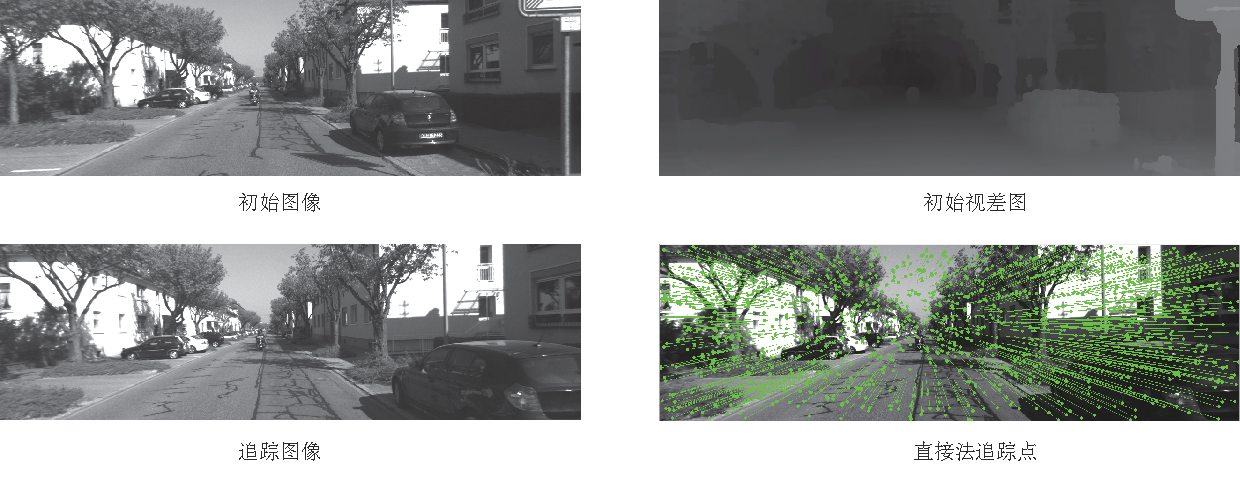
\includegraphics[width=1.0\linewidth]{vo2/direct-experiment}
	\caption{Experimental results of the direct method. upper left: original image; upper right: disparity map corresponding to the original image; lower left: fifth tracking image; lower right: tracking result}
	\label{fig:direct-experiment}
\end{figure}

Below we briefly explain the iterative process of the direct method. Compared with the feature point method, the direct method completely relies on the optimization to solve the camera pose. It can be seen from the formula \eqref{eq:jacobianofDirect} that the pixel gradient guides the direction of optimization. If you want to get the correct optimization results, you must ensure that \textbf{most pixel gradients can guide the optimization in the right direction}.

What does it mean? Assume that for the reference image, we measured a pixel with a gray value of 229. And, since we know its depth, we can infer the position of the space point $P$ (\autoref{fig:directExperiment}~shown as the grayscale measured in $I_1$).

\begin{figure}[!htp]
	\centering
	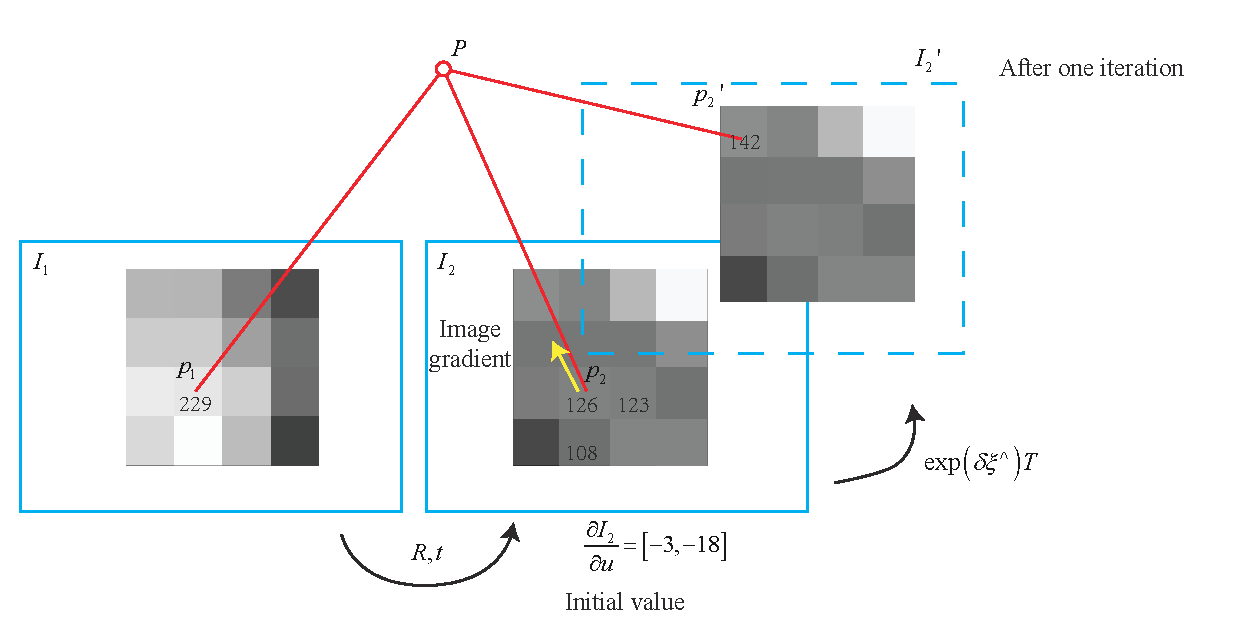
\includegraphics[width=.9\linewidth]{vo2/directExperiment}
	\caption{workflow of one iteration.}
	\label{fig:directExperiment}
\end{figure}

Now, we have got a new image and need to estimate its camera pose. This pose is obtained by continuous optimization iterations of an initial value. Assuming that our initial value is relatively poor, under this initial value, the pixel gray value after the projection of the space point $P$ is 126. Therefore, the error of this pixel is $229-126=103$. In order to reduce this error, we hope to \textbf{fine-tune the camera's pose to make the pixels brighter}.

How do I know where to fine-tune the pixels to make them brighter? This requires the use of local pixel gradients. We found in the image that if we take a step forward along the $u$ axis, the gray value at that point becomes 123, that is, 3 is subtracted. Similarly, if you take a step forward along the $v$ axis, the gray value is reduced by 18 and becomes 108. Around this pixel, we see that the gradient is $[-3,-18]$. In order to increase the brightness, we will suggest optimizing the algorithm to fine-tune the camera so that the image of $P$ moves to \textbf{top left}. In this process, we use the local gradient of the pixel to approximate the grayscale distribution near it, but please note that the real image is not smooth, so this gradient is not valid at a distance.

However, the optimization can't just follow the behavior of just one pixel, but also need to get track of other pixels. After considering many pixels, the optimization algorithm chose a place not far from the direction we suggested, and calculated an update amount $\exp ({\mathbf{\xi}^\wedge} )$. After adding the update amount, the image has moved from $I_2$ to $I_2'$, and the projection position of the pixel has also changed to a brighter place. We see that with this update, \textbf{error has become smaller}. Under ideal circumstances, we expect the error to continue to decrease and eventually converge.

But is this actually the case? Do we really only need to walk along the gradient direction to reach an optimal value? Note that the gradient of the direct method is directly determined by the image gradient, so we must ensure that \textbf{when walking along the image gradient, the photometric error will continue to decrease}. However, the image is usually a very strong \textbf{non-convex function}, as shown in \autoref{fig:non-convex}~. In practice, if we move along the image gradient, it is easy to fall into a local minimum due to the non-convexity (or noise) of the image itself, and we cannot continue to optimize. The direct method can only be established when the camera movement is very small and the gradient in the image will not have strong non-convexity.

\begin{figure}[!htp]
	\centering
	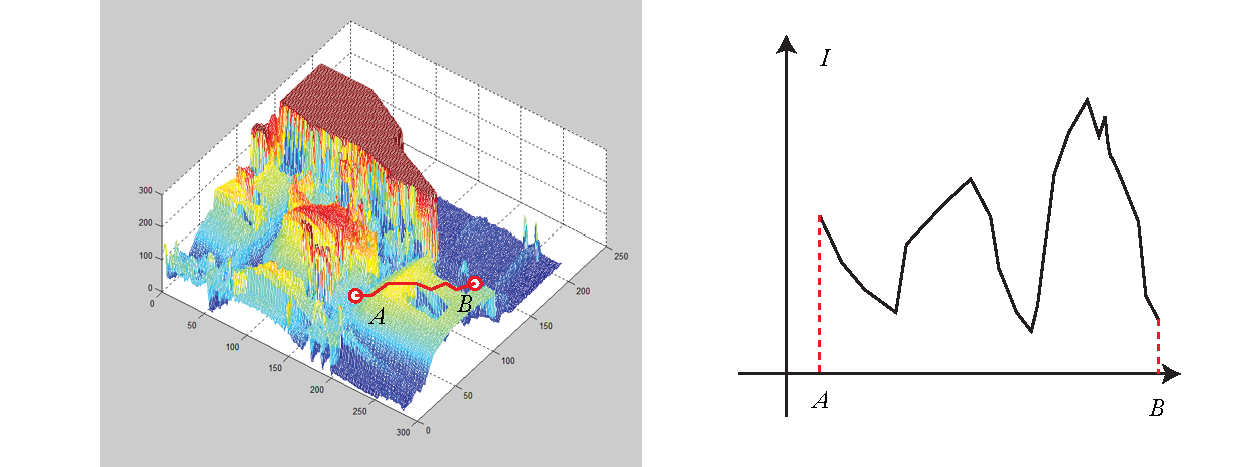
\includegraphics[width=1.0\linewidth]{vo2/nonconvex}
	\caption{Three-dimensional visualization of an image. The path from one point in the image to another point is not necessarily a "straight downhill road", but needs to be "climbing over the mountains" frequently. This reflects the non-convexity of the image itself.}
	\label{fig:non-convex}
\end{figure}

In the example, we only calculated the difference of a single pixel, and this difference is obtained by directly subtracting the grayscale. However, a single pixel is not distinguishable, and there are probably many pixels around with similar brightness. Therefore, we sometimes use small patches and use more complex difference measures, such as Normalized Cross Correlation (NCC). For the sake of simplicity, the example uses the sum of squares of errors to maintain consistency with the derivation.

\subsection{Advantages and disadvantages of the direct method}
Finally, we summarize the advantages and disadvantages of the direct method. In general, its advantages are as follows:

\begin{itemize}
	\item It can save the time of calculating feature points and descriptors.
	\item Only pixel gradients are required, no feature points are required. Therefore, the direct method can be used in the absence of features. An extreme example is an image with only gradients. It may not be able to extract corner features, but its motion can be estimated by a direct method. In the demonstration experiment, we see that the direct method can also work normally for randomly selected points. This is very important in practice, because practical scenes may not have many corner points to use.。
	\item It is possible to construct semi-dense or even dense maps, which cannot be achieved by the feature point method.
\end{itemize}

On the other hand, its shortcomings are also obvious:
\begin{itemize}
	\item \textbf{Non-convexity}. The direct method completely relies on gradient search and reduces the objective function to calculate the camera pose. The objective function needs to take the gray value of the pixel, and the image is a strongly non-convex function. This makes the optimization algorithm easy to be stuck at a local minimum, and the direct method can only succeed when the movement is small. Against this, the pyramids can reduce the impact of non-convexity to a certain extent.
	\item \textbf{Single pixel has no discriminativeness}. Many points look alike. So we either calculate image patches or calculate complex correlations. Since each pixel has inconsistent "opinions" about changing the camera movement, only a few obey the majority, and increasing the quantity for better quality. Therefore, the performance of the direct method decreases significantly when there are fewer selected points. We usually recommend using more than 500 points.
	\textbf{Brightness constant is a strong assumption}. If the camera is automatically exposed, when it adjusts the exposure parameters, it will make the overall image brighter or darker. This situation also occurs when the light changes. The feature point method has a certain tolerance to illumination, while the direct method calculates the difference of brightness, and the overall brightness change will destroy the brightness constant assumption and make the algorithm fail. In response to this, the practical direct method will also estimate the camera's exposure parameters \cite{Engel2016} so that it can still work when the exposure time changes.
\end{itemize}

\section*{习题}
\begin{enumerate}
	\item In addition to LK optical flow, do you know other optical flow methods? What are their characteristics?
	\item In the program to calculate the image gradient, we simply calculate the difference between the brighteness of $u+1$ and $u-1$ divided by 2 as the gradient in the direction of $u$. What are the disadvantages of this approach? Hint: For features closer together, the changes should be faster; while for features farther away it changes more slowly in the image, can this information be used when calculating the gradient?
	\item Can the direct method be implemented in an "inverse" way like optical flow? That is, use the gradient of the original image instead of the gradient of the target image?
	\item[\optional] Use Ceres or g2o to implement sparse direct method and semi-dense direct method.
	\item Compared with the direct method of RGB-D, the monocular direct method is often more complicated. In addition to the unknown matching, the pixel distance is also to be estimated, and we need to use the pixel depth as an optimization variable during optimization. Refer to the literature \cite{Engel2013, Engel2014}, can you understand its principle?
\end{enumerate}



% !Mode:: "TeX:UTF-8"
\chapter{Backend: Part I}
\label{cpt:backend1}
\begin{mdframed}  
	\textbf{Goal of Study}
	\begin{enumerate}[labelindent=0em,leftmargin=1.5em]
		\item Learn how to formulate the backend problem into a filter or least square optimization problem.
		\item Learn how to use the sparse structure in bundle adjustment problem. 
		\item Solve a BA problem with g2o and Ceres.
	\end{enumerate}
\end{mdframed}

From this lecture, we turn to another important module: back-end optimization.
We see that the front-end visual odometry can give a short-term trajectory and map. Still, due to the inevitable accumulation of errors, this map is inaccurate for a long time. Therefore, based on visual odometry, we also hope to construct a larger-scale optimization problem to consider the optimal trajectory and map over a long time. However, considering the balance of accuracy and performance, there are many different approaches in practice.

\newpage
\includepdf{resources/other/ch10.pdf}

\newpage
\section{Introduction}
\subsection{State Estimation from Probabilistic Perspective}
As mentioned in the second lecture, the visual odometry only has a short memory, but we hope that the system can maintain the entire motion trajectory in an optimal state for a long time. We may use the latest knowledge to update an old state. At that time, it seems that future information tells you, ``where you should be now.'' Therefore, in the back-end optimization, we usually consider the problem of state estimation for a longer period of time (or all-time), and not only use the past information to update our current state but also use future information to update ourselves. Such a method might be called ``Batch.'' Otherwise, if the current state is only determined by the past, or even only by the previous moment, it might also be called ``Incremental.''

We already know that the SLAM process can be described by the motion and observation equations. Suppose in the time from $t=0$ to $t=N$, we have the poses from $\bm{x}_0$ to $\bm{x}_N$ and observation $\bm{y}_1, \cdots, \bm{y}_M$. According to the equations in chapter 2, we write them as: 
\begin{equation}
	\left\{ \begin{array}{l}
		{\bm{x}_k} = f\left( {{\bm{x}_{k - 1}},{\bm{u}_k}} \right) + \bm{w}_k \\
		{\bm{z}_{k,j}} = h\left( {{ \bm{y}_j},{ \bm{x}_k}}  \right)+ \bm{v}_{k,j}
	\end{array} \right. \quad k=1, \ldots, N, \  j=1, \ldots, M.
\end{equation}

Note that in the SLAM problem we have the following characteristics:
\begin{enumerate}
	\item In the observation equation, only when $\bm{x}_k$ sees $\bm{y}_j$, we will have a real observation equation. In fact, we can usually see only a small part of the landmarks in one location. Moreover, due to a large number of visual SLAM feature points, the number of observation equations in practice will be much larger than that of motion equations.
	\item We may not have a device to measure motion, so there may not be a motion equation. In this case, there are several ways to deal with it:
	\begin{itemize}
		\item Assume that there is really no motion equation.
		\item Assume that the camera does not move.
		\item Assume that the camera is moving at a constant speed.
	\end{itemize}
	These several methods are all feasible. In the absence of motion equations, the entire optimization problem consists of only observation equations. This is very similar to the SfM (Structure from Motion) problem, which is equivalent to restoring the motion and structure through a set of images. The difference with SfM is that the images in SLAM have a chronological order, while SfM allows the use of completely unrelated images.
\end{enumerate} 

We know that every measurement is affected by noise, so the poses $\bm{x}$ and landmarks $\bm{y}$ here are regarded as \textbf{random variables that obey a certain probability distribution} instead of a single number. Therefore, the question becomes: when I have some motion data $\bm{u}$ and observation data $\bm{z}$, how to determine the state $\bm{x}$ and landmarks $\bm{y}$'s distribution? Furthermore, if new data is obtained, how to update our estimation? In more common and reasonable cases, we assume that the state quantity and noise terms obey Gaussian distribution-which means that only their mean and covariance matrix need to be stored in the program. The mean can be regarded as an estimate of the state variable's optimal value, and the covariance matrix measures its uncertainty. Then, the question becomes: when there are some motion and observation data, how do we estimate the Gaussian distribution of the states?

We still put ourselves in the role of a robot. When there is only the equation of motion, it is equivalent to walking blindfolded in an unknown place. Although we know how far we have taken for each step, we will become more and more uncertain about where we are as time grows. This reflects that when the input data is affected by noise, the error is gradually accumulated, and our estimate of the position variance will become larger and larger. However, when we open our eyes, we will become more and more confident because we can continuously observe the external scene, making the uncertainty of position estimation smaller. If we use an ellipse to intuitively express the covariance matrix, then this process is a bit like walking in a mobile phone map software. Taking \autoref{fig:uncertainty}~ as an example, readers can imagine that when there is no observation data, the circle will become larger and larger with the movement; and if there are correct observations, the circle will shrink to a certain size and keep stable.

\begin{figure}[!ht]
	\centering
	\includegraphics[width=0.66\textwidth]{backend1/uncertainty.pdf}
	\caption{An intuitive description of uncertainty. Left: When there is only the motion equation, the pose at the next moment adds noise to the previous moment, so the uncertainty is getting bigger and bigger. Right: When there are road signs, the uncertainty will be significantly reduced. Please note that this is only an intuitive diagram, not actual data.}
	\label{fig:uncertainty}
\end{figure}

The above statements explain the problem of state estimation in a metaphorical form. Below we will look at it in a quantitative way. In Lecture \ref{cpt:6}, we introduced the maximum likelihood estimation where we say that the problem of \textbf{batch state estimation} can be transformed into a \textbf{maximum likelihood estimation problem and solved by the least square method}. In this section, we will explore how to apply this conclusion to progressive problems and get some classic conclusions. At the same time, we will investigate the special structure of the least square method in visual SLAM.



% !Mode:: "TeX:UTF-8"
\chapter{Filters and Optimization Approaches: Part II}
\label{cpt:backend2}
\begin{mdframed}  
	\textbf{Goal of Study}
	\begin{enumerate}[labelindent=0em,leftmargin=1.5em]
		\item Learn the principles of sliding window optimization; 
		\item Learn the basic knowledge about pose graph optimization.
		\item Pose graph optimization with \textit{g2o}.
	\end{enumerate}
\end{mdframed}

In the last lecture, we focused on graph optimization based on BA. BA can accurately optimize the pose and feature point position of each camera. However, in a larger scene, the high dimensionality of landmarks will seriously reduce the calculation efficiency, resulting in an increasing amount of calculation that cannot be real-time. The first part of this lecture will introduce a simplified, yet widely used optimization approach: pose graph.

\newpage
\section{Sliding Window Filter and Optimization}
\subsection{Controlling the Structure of BA}

The graph optimization with camera pose and spatial points is called BA, which can effectively solve large-scale positioning and mapping problems. This is very useful in SfM, but in the real-time SLAM process, we often need to control the problem's scale to maintain real-time calculations. If the computing power is unlimited, we might calculate the entire BA every moment-but that does not meet the reality. The reality is that we must limit the calculation time of the backend. For example, the BA scale cannot exceed 10,000 landmarks, the iterations cannot exceed 20 times, and the time used does not exceed 0.5 seconds, and so on. An algorithm that takes a week to reconstruct a city map like SfM is not necessarily effective in SLAM.

There are many ways to control the calculation scale, such as extracting keyframes from the continuous video~\cite{Leutenegger2015}, only constructing the BA between the keyframe and the landmarks. The non-keyframes are only used for localization and do not contribute to the mapping part. Even so, as time goes by, the number of keyframes will increase, and the scale of the map will continue to grow. For batch optimization methods like BA, the computational efficiency will (worryingly) continue to decline. To avoid this situation, we need to control the scale of the backend problem. These methods can be theoretical or engineering.

For example, the simplest way to control the BA scale is to keep only the $N$ keyframes closest to the current moment and remove the earlier ones. Therefore, we will fix the BA within a time window, and those that leave this window will be discarded. This method is called the sliding window method~\cite{Sibley2008}. Of course, we can change the criteria for selecting these $N$ keyframes. For example, it is unnecessary to take the closest in time, but according to a certain principle, take the keyframes that are close in time and expandable in space. To ensure that even when the camera is stopped, the BA structure will not shrink into a single point (this can easily lead to some bad degradation). If we think more deeply about the structure of frames and frames, we can also define a structure called ``covisibility graph'' like ORB-SLAM2~\cite{Mur-Artal2015} (see \autoref{fig:cov-graph}). The so-called co-visibility refers to those features that are observed together with the current keyframe). Therefore, in BA optimization, we take some keyframes and landmarks in the co-visibility graph to optimize. For example, we may pick about 20 co-visible keyframes with the current frame and leave the others unchanged. If we can construct the co-visibility relationship correctly, the optimization will remain optimal for a longer time.

\begin{figure}[!ht]
	\centering
	\includegraphics[width=0.8\textwidth]{backend2/cov-graph.pdf}
	\caption{Co-visibility graph in sliding window. }
	\label{fig:cov-graph}
\end{figure}

No matter whether it is a sliding window or a co-visibility approach, in general, it is a kind of engineering trade-off between full SLAM and real-time computing. But in theory, they also introduce a new problem: when we talk about "discarding" variables outside the sliding window or "fixing" variables outside the co-visibility graph, what is the specific operation of "discarding" and "fixing"? "Fixed" seems to be easy to understand. We only need to keep the keyframe estimates unchanged during optimization. But "discarding" refers to completely abandoning it, which means that the variables outside the window totally do not affect the variables in the window?  Or does the data outside the window should have some influence but is somehow ignored? 

Next, we will talk about these issues. How should they be dealt with in theory, and whether can we simplify them in engineering?

\subsection{Sliding Window}
Now consider a sliding window. Assume there are $N$ keyframes in this window, and their poses are denoted as $$\bm{x}_1, \ldots, \bm{x}_N,$$ we assume that they are in the vector space, that is, using Lie Algebra expression, then, what can we talk about these keyframes?

Obviously, we care about the location of these keyframes and their uncertainty. This corresponds to their mean and covariance under the assumption of Gaussian distribution. If these keyframes also correspond to a local map, we can also ask for the entire local map's mean and covariance. Suppose there are $M$ landmark points in this sliding window: $\bm{y}_1, \ldots, \bm{y}_N$, they form a local map together with the $N$ keyframes. Obviously, we can use the bundle adjustment method introduced in the last lecture to deal with this sliding window, including building a graph optimization model, building an overall Hessian matrix, and then marginalizing all landmarks to speed up the solution. After the marginalization, we get the conditional distribution of the poses, namely $$[\bm{x}_1, \ldots, \bm{x}_N | \bm{y}_1, \ldots, \bm{y}_M ] \sim N([\boldsymbol{\mu }_1, \ldots, \boldsymbol{\mu}_N]^T, \boldsymbol{\Sigma}).$$ where $\boldsymbol{\mu}_k$ is mean of the $k$-th keyframe, $\boldsymbol{\Sigma}$ is the covariance matrix of all keyframes. So obviously, the mean part refers to the optimal result after BA, and $\boldsymbol{\Sigma}$ is the result of the marginalization, i.e., the matrix $\bm{S}$ mentioned in the previous lecture. We think that readers are already familiar with this process.

In a sliding window, another question is to ask, when the window moves, how should these state variables change? This matter can be discussed in two parts:

\begin{enumerate}
	\item We want to add a new keyframe into the window as well as its corresponding landmarks.
	\item We need to delete an old keyframe in the window, and may also delete the landmarks it observes.
\end{enumerate}

At this time, the difference between the sliding window method and the traditional BA is revealed. If processed as a traditional BA, then this only corresponds to two BAs with different structures, and there is no difference in the solution. But in the case of sliding windows, we have to discuss these specific details.

\subsubsection{Adding New Keyframes}
Considering that the sliding window has established $N$ keyframes at the last moment, and we already know that they obey a certain Gaussian distribution, and their mean and variance are as described above. At this time, a new keyframe $\bm{x}_{N+1}$ has arrived, and the variables in the whole problem become a collection of $N+1$ keyframes and more road signs. In fact, this is still ordinary. We only need to follow the normal BA process. When all points are marginalized, the Gaussian distribution of these $N+1$ keyframe poses are obtained.

\subsubsection{Removing Old Keyframes}
When considering deleting old keyframes, a theoretical problem will emerge. For example, we want to delete the old keyframe $\bm{x}_1$. But $\bm{x}_1$ is not isolated. It will observe the same landmarks as other frames. After marginalizing $\bm{x}_1$, the whole problem will no longer be sparse. As in the previous lecture, let's take a schematic diagram, as shown in \autoref{fig:marg-frame}.

\begin{figure}[!ht]
	\centering
	\includegraphics[width=1.0\textwidth]{backend2/marg-frame.pdf}
	\caption{Margining old keyframes will break the sparse structure of the Hessian.}
	\label{fig:marg-frame}
\end{figure}

In this example, we assume that $\bm{x}_1$ sees the landmarks from $\bm{y}_1$ to $\bm{y}_4$, so before processing, the Hessian matrix of the BA problem should be like the left side of this figure. There are non-zero blocks in the columns $\bm{y}_1$ to $\bm{y}_4$ in the $\bm{x}_1$ row, which means $\bm{x}_1 $ saw them. At this time, consider the marginalization $\bm{x}_1$. Please recall what we do in the Schur trick: We multiply the first row by the coefficient and adding it to the rows below the dividing line to eliminate the non-zero block in the first column; then use the first column to eliminate the non-zero block in the first row. But when we do this, the Hessian of the Landmark-Landmark part is filled with information by this operation, and it is no longer a diagonal block. This phenomenon is called (fill in) {\cite{Sibley2008}}.

Intuitively, fill-in means that when you ask for $P(\bm{x}_2, \bm{x}_3, \bm{x}_4, \bm{y}_1, \ldots \bm{y}_4|\bm{x}_1)$, because the marginalized keyframe sees some landmarks, these landmarks have one more constraint saying ``where they should be if $\bm{x}_1$ is set to the current value" (conditional distribution).Such a priori constraint describes the information about where these landmarks should be.

Recalling the marginalization mentioned in the previous lecture, when we marginalize the landmarks, the fill-in effect will appear in the pose block in the upper left corner. However, because BA does not require the pose block to be a diagonal block, the sparse BA solution is still feasible. However, when the keyframes are marginalized, it will destroy the diagonal block structure between the landmark points in the lower right corner. We cannot solve BA iteratively in the previous sparse method. This is obviously a terrible question. In fact, in the backend of the early EKF filter, people did maintain a dense Hessian matrix, which also made the backend of the EKF unable to handle higher dimension states.

However, if we make some modifications to the marginalization process, we can also maintain the sliding window BA's sparsity. For $\bm{y}_1$ to $\bm{y}_4$, they may fall into the three cases listed below:

\begin{enumerate}
	\item The landmark is only observed in $\bm{x}_1$ and does not appear in the remaining keyframes. Then you can just throw away the landmark without any impact on the window. This landmark is isolated.
	\item The landmark is seen in $\bm{x}_2$-$\bm{x}_4$, but will not be seen in the future. (This is just an assumption here, and it actually depends on the implementation of the frontend. Optical flow frontends like VINS~\cite{Qin2018} or DSO will not track the missing feature points, so we can just assume this is the case.) Then you can also marginalize this landmark. When road signs are marginalized, a priori of the pose-pose part is generated, so it becomes the prior information of the future pose estimation.
	\item The landmark is seen in $\bm{x}_2$-$\bm{x}_4$ and may be seen in the future. Then this landmark should not be marginalized, because we will need to update its estimate later. In theory, we can only maintain the dense structure in the landmark-landmark part, but in engineering, we can pretend that the observation of this landmark by $\bm{x}_1$ can be simply discarded (equivalent to thinking that $\bm{x}_1$ did not see it). So we kept the diagonal structure of the Landmark part at a small cost. In this case you don't have to do anything.
\end{enumerate}


\subsubsection{Intuitive Explanation of the Marginalization in SWF}
We know that the meaning of marginalization in probability refers to decomposing a joint distribution into a conditional and marginal distribution. So intuitively speaking, when we marginalize a keyframe, we mean ``keep the current estimated value of this keyframe and find the conditional probability of other state variables conditioned on this keyframe.'' Therefore, when a keyframe is marginalized, the landmark points it observes will generate a priori information of ``\textbf{where these landmarks should be},'' which affects the estimated value of the rest. If these landmark points are then marginalized, their observers will get a priori information of ``\textbf{where the keyframe to observe them should be}.''

Mathematically, when we marginalize a certain keyframe, the description of the state variables in the entire window will change from a joint distribution to a conditional probability distribution. Taking the example above, it means:
\begin{equation}
	p\left( {{\bm{x}_1}, \ldots {\bm{x}_4},{\bm{y}_1}, \ldots {\bm{y}_6}} \right) = p\left( {{\bm{x}_2}, \ldots ,{\bm{x}_4},{\bm{y}_1}, \ldots {\bm{y}_6}|{\bm{x}_1}} \right)\underbrace {p\left( {{\bm{x}_1}} \right)}_{\text{discarded}}.
\end{equation}
Then discard the marginalized part of the information. After the variable is marginalized, we should no longer use it in engineering. Therefore, the sliding window method is more suitable for VO systems but not for large-scale mapping systems.

Since \textit{g2o} and Ceres have not explicitly supported the marginal operation in the sliding window method \footnote{In the project, we can walk around \textit{g2o} and Ceres's restrictions through some clever tricks, but this is often very troublesome and not suitable for demos. }, we omit the corresponding experimental part in this section. I hope the theoretical part can help readers understand some SLAM systems based on sliding windows.

\section{Pose Graph Optimization}
\subsection{Definition of Pose Graph}
According to the previous discussion, we found that landmarks occupy most of the optimization time. In fact, after several observations, the spatial position of the landmarks will converge to a value and remain almost unchanged, while the divergent outliers are usually invisible. Optimizing the convergent landmarks seems a bit useless. Therefore, we are more inclined to fix the feature points after a few iterations and only regard them as constraints of pose estimation instead of actually optimizing their position.

Following this idea, we will think: Can we ignore the landmarks at all and only focus on the poses? We can construct a graph optimization with only pose variables. The edge between the pose vertices can be set with measurement by the ego-motion estimation obtained from feature matching. The difference is that once the initial estimation is completed, we no longer optimize the positions of those landmark points but only care about the connections between all camera poses. In this way, we save a lot of calculations for landmarks optimization and only keep the keyframe's trajectory, thus constructing the so-called pose graph (Pose Graph), shown in \autoref{fig:pose-graph}.

\begin{figure}[!ht]
	\centering
	\includegraphics[width=0.8\textwidth]{backend2/posegraph.pdf}
	\caption{Pose Graph diagram. When we no longer optimize the landmark in Bundle Adjustment, and only regard them as constraints on the pose nodes, we get a pose graph with a much reduced calculation scale.}
	\label{fig:pose-graph}
\end{figure}

We know that the number of landmarks in BA is much greater than that of pose nodes. A keyframe is often associated with hundreds of key points. Even if the sparsity is used, the maximum calculation scale of real-time BA is generally around tens of thousands of points on the current mainstream CPU. This limits the application scenarios of SLAM. Therefore, when the robot moves in a larger range of time and space, we must consider some solutions: Either discard some historical data like the sliding window method {\cite{Strasdat2011}}; or like the usage of pose graph, abandon the optimization of landmark, and only keep the edges between pose variables {\cite{Dubbelman2015, Lee2014, Latif2013}}. Besides, if we have additional sensors to measure pose (GPS, UWB), then the pose graph is also a common method of fusing pose measurements.

\subsection{Residuals and Jacobians}
So, how do we define the vertices and edges in a pose graph optimization? The node here represents the camera pose, expressed in $\bm{T}_1, \cdots, \bm{T}_n$. The edge is the estimation of the relative motion between the two pose nodes. The estimation may come from the feature point method or the direct method, or GPS or IMU integration, but no matter what, we estimate it, for example, a movement between $\bm{T}_i$ and $\bm{T}_j$ is $\Delta \bm{T}_{ij}$. We can express the movement in several ways. Let's take the a natural one:

\begin{equation}
	\Delta \bm{\xi}_{ij} = \bm{\xi}_i^{-1} \circ \bm{\xi}_j = \ln \left( \bm{T}_i^{-1} \bm{T}_j \right)^\vee,
\end{equation}

Or in $\mathrm{SE}(3)$'s manner:
\begin{equation}
	\bm{T}_{ij} =\bm{T}_i^{-1} \bm{T}_j.
\end{equation}

According to the principle of graph optimization, the equation will not hold exactly in practice. Hence, we set up the least-square error and then, as before, discuss the derivative of the error with respect to the optimized variable. Here, we move the $\bm{T}_{ij}$ of the above equation to the right side of the equation to construct the error $\bm{e}_{ij}$:
\begin{equation}
	\bm{e}_{ij} = \Delta \bm{\xi}_{ij} \ln \left( \bm{T}_{ij}^{-1} \bm{T}_i^{-1} \bm{T}_j \right)^\vee
\end{equation}

Note that there are two optimization variables: $\bm{\xi}_i$ and $\bm{\xi}_j$, so we find the derivative of $\bm{e}_{ij}$ about these two variables. According to the derivation method of Lie algebra, give $\bm{\xi}_i$ and $\bm{\xi}_j$ a left disturbance: $ \bm{\delta \xi}_i$ and $\bm{\delta \xi}_j$. Then the error becomes:
\begin{equation}
	\hat{ \bm{e}}_{ij} = \ln \left( \bm{T}_{ij}^{-1}  \bm{T}_i^{-1} \exp((-\bm{\delta \xi}_i)^\wedge) \exp(\delta \bm{\xi}_j^\wedge) \bm{T}_j  \right)^\vee.
\end{equation}

In this formula, the two disturbance terms are placed in the middle. We want to move the disturbance term to the equation's left or right side to use the BCH approximation. Recall the adjoint property in the fourth lecture, which is the formula \eqref{eq:adjSE3}. If you have not done this exercise before, use it as the correct conclusion for now:
\begin{equation}
	\exp \left( \left( \mathrm{Ad}(\bm{T}) \bm{\xi} \right) ^\wedge \right) = \bm{T} \exp(\bm{\xi}^\wedge)\bm{T}^{-1}.
\end{equation}

Rearrange it:
\begin{equation}
	\exp(\bm{\xi}^\wedge)\bm{T} = \bm{T} \exp \left( \left( \mathrm{Ad}(\bm{T}^{-1}) \bm{\xi} \right) ^\wedge \right) .
\end{equation}

This formula shows that by introducing an adjoint term, we can "exchange" the $\bm{T}$ on the left and right sides of the disturbance term. With this property, the disturbance terms can be moved to the right (of course, the left is also possible), and the Jacobian matrix in the form of right multiplication (left multiplication is formed when moved to the left):

\begin{equation}
	\begin{aligned}
		\hat{ \bm{e}}_{ij} &= \ln \left( \bm{T}_{ij}^{-1}  \bm{T}_i^{-1} \exp((-\bm{\delta \xi}_i)^\wedge) \exp(\delta \bm{\xi}_j^\wedge) \bm{T}_j  \right)^\vee\\
		&= \ln \left( \bm{T}_{ij}^{-1} \bm{T}_i^{-1} \bm{T}_j \exp \left( \left(- \mathrm{Ad}(\bm{T}_j^{-1}) \bm{\delta \xi}_i \right)^\wedge \right) \exp \left( \left( \mathrm{Ad}(\bm{T}_j^{-1})  \bm{\delta\xi}_j\right)^\wedge \right) \right)^\vee \\ 
		&\approx \ln \left( \bm{T}_{ij}^{-1} \bm{T}_i^{-1} \bm{T}_j \left[ \bm{I} - (\mathrm{Ad}(\bm{T}_j^{-1}) \bm{\delta \xi}_i)^\wedge + (\mathrm{Ad}(\bm{T}_j^{-1})  \bm{\delta \xi}_j)^{\wedge} \right] \right)^\vee \\
		& \approx \bm{e}_{ij} + \frac{\partial \bm{e}_{ij}}{\partial \bm{\delta \xi}_i} \bm{\delta \xi}_i + \frac{\partial \bm{e}_{ij}}{\partial \bm{\delta \xi}_j} \bm{\delta \xi}_j
	\end{aligned},
\end{equation}
where the two Jacobians are:
\begin{equation}
	\frac{\partial \bm{e}_{ij}}{\partial \bm{\delta \xi}_i} = - \bm{\mathcal{J}}_r^{-1}(\bm{e}_{ij}) \mathrm{Ad}(\bm{T}_j^{-1}) 
\end{equation}
and
\begin{equation}
	\frac{\partial \bm{e}_{ij}}{\partial \bm{\delta \xi}_j} = \bm{\mathcal{J}}_r^{-1}(\bm{e}_{ij}) \mathrm{Ad}(\bm{T}_j^{-1}).
\end{equation}

If readers find it difficult to understand the derivation of this part, please return to lecture 4 to review the content of $\mathrm{SE}(3)$. However, as mentioned earlier, because the left and right Jacobian $\bm{\mathcal{J}}_r$ forms on $\mathfrak{se}(3)$ are too complicated, we usually approximate them. If the errors are close to zero, we can set them approximately as $\bm{I}$ or as:
\begin{equation}
	\bm{\mathcal{J}}_r^{-1}(\bm{e}_{ij}) \approx \bm{I} + \frac{1}{2} 
	\left[ 
	{\begin{array}{*{20}{c}}
			{{\bm{\phi}_{\bm{e}} ^ \wedge }}&{{\bm{\rho}_{\bm{e}} ^ \wedge }}\\
			{\bm{0}}&{{\bm{\phi}_{\bm{e}} ^ \wedge }}
	\end{array}} 
	\right].
\end{equation}

Theoretically speaking, even after optimization, since the observation data given by each edge is not consistent, the error is usually not close to zero, so simply setting the $\bm{\mathcal{J}}_r$ here as $\bm{I}$ will have an inevitable loss. Later we will see through practice to see if the theoretical difference is noticeable.

After understanding the Jacobian derivation, the rest is the same as ordinary graph optimization. In short, all pose vertices and pose edges constitute a graph optimization, which is essentially a least-squares problem. The optimization variable is the pose of each vertex, and the edges come from the pose observation constraints. Let $\mathcal{E}$ be the set of all edges, then the overall objective function is:
\begin{equation}
	\mathop {\min }\limits \frac{1}{2}\sum\limits_{i,j \in \mathcal{E}} \bm{e}_{ij}^T \bm{\Sigma}_{ij}^{-1} \bm{e}_{ij}.
\end{equation}

After understanding the Jacobian derivation, the rest is the same as ordinary graph optimization. In short, all pose vertices and pose edges constitute a graph optimization, which is essentially a least-squares problem. The optimization variable is the pose of each vertex, and the edges come from the pose observation constraints. Let $\mathcal{E}$ be the set of all edges, then the overall objective function is

We can still use Gauss Newton's method, the Levenberg-Marquardt method, etc., to solve this problem.  Based on previous experience, we can naturally solve this with Ceres or \textit{g2o}. We won't discuss the detailed process of optimization anymore. We have talked about enough in the last lecture.

\section{Practice: Pose Graph}
\subsection{Pose Graph Using \textit{g2o} Built-in Classes}
Now let's demonstrate the use of \textit{g2o} to optimize the pose graph. First of all, please use \textit{g2o\_viewer} command to open our pre-generated simulation pose graph, located in ``slambook2/ch10/sphere.g2o'', as shown in \autoref{fig:sphere-before}~.

\begin{figure}[!htp]
	\centering
	\includegraphics[width=1.0\textwidth]{backend2/sphere-before.pdf}
	\caption{Pose graph generated by simulation. The true value is a perfect sphere. After adding noise to the true value, the simulation data with accumulated error is obtained.}
	\label{fig:sphere-before}
\end{figure}

The pose graph is simulated by the create sphere program that comes with \textit{g2o}. Its ground-truth trajectory is a ball composed of multiple layers from bottom to top. Each layer is a perfect circle. Many circular layers of different sizes form a complete sphere, which contains 2500 pose nodes (\autoref{fig:sphere-before}~upper left). Then, the simulation program generates odometry edges from $t-1$ to $t$. The edges between layers are also generated, called loop closure edges (loop detection algorithm will be introduced in detail in the next lecture). Then, we add observation noise to each edge and reset the initial value of the node according to the noisy initial value of the odometry edge. In this way, the pose graph data will be affected by accumulative error (\autoref{fig:sphere-before}~bottom right). It looks like part of a sphere locally, but the overall shape is far from that of a sphere. Now we start from the initial values of these noisy edges and nodes, optimize the entire pose graph, and get data that approximates the true value.

Of course, the real robot will certainly not have such a spherical motion trajectory and complete odometry and loop observation data. The advantage of the simulation into a perfect sphere is that we can intuitively see whether the optimization result is correct (as long as to see it is round or not). Readers can click the optimize function in \textit{g2o\_viewer} to see the optimization results and convergence process of each step. On the other hand, sphere.g2o is also a text file. You can open it with a text editor to view its contents. The first half of the file is composed of nodes, and the second half is edges:

\begin{lstlisting}
	VERTEX_SE3:QUAT 0 -0.125664 -1.53894e-17 99.9999 0.706662 4.32706e-17 0.707551 -4.3325e-17 
	......
	EDGE_SE3:QUAT 1524 1574 -0.210399 -0.0101193 -6.28806 -0.00122939 0.0375067 -2.85291e-05 0.999296 10000 0 0 0 0 0 10000 0 0 0 0 10000 0 0 0 40000 0 0 40000 0 40000 
\end{lstlisting}

As you can see, the node type is VERTEX\_SE3, which expresses a camera pose. \textit{g2o} uses quaternion and translation vector to describe the pose by default, so the meaning of the following fields are ID, $t_x, t_y, t_z, q_x, q_y, q_z, q_w$. The first 3 are translation vector elements, and the last 4 are unit quaternions that represent rotation. Similarly, the edge information is the ID of the two nodes, $t_x, t_y, t_z, q_x, q_y, q_z, q_w$, the upper right corner of the information matrix (because the information matrix is a symmetric matrix, you only need to save half of it). You can see that the information matrix is set to a diagonal matrix.

In order to optimize the pose graph, we can use the default vertices and edges of \textit{g2o}, which are represented by quaternions. Since the simulation data is also generated by \textit{g2o}, optimization by \textit{g2o} itself does not require us to do any more work. Just configure the optimization parameters. The program slambook2/ch10/pose\_graph\_g2o\_SE3.cpp demonstrates how to use the Levenberg-Marquardt method to optimize the pose image and store the result in the result.g2o file.

\begin{lstlisting}[language=c++,caption=slambook2/ch10/pose\_graph\_g2o\_SE3.cpp]
#include <iostream>
#include <fstream>
#include <string>

#include <g2o/types/slam3d/types_slam3d.h>
#include <g2o/core/block_solver.h>
#include <g2o/core/optimization_algorithm_levenberg.h>
#include <g2o/solvers/eigen/linear_solver_eigen.h>

using namespace std;

int main(int argc, char **argv) {
	if (argc != 2) {
		cout << "Usage: pose_graph_g2o_SE3 sphere.g2o" << endl;
		return 1;
	}
	ifstream fin(argv[1]);
	if (!fin) {
		cout << "file " << argv[1] << " does not exist." << endl;
		return 1;
	}
	
	// setting up g2o
	typedef g2o::BlockSolver<g2o::BlockSolverTraits<6, 6>> BlockSolverType;
	typedef g2o::LinearSolverEigen<BlockSolverType::PoseMatrixType> LinearSolverType;
	auto solver = new g2o::OptimizationAlgorithmLevenberg(
		g2o::make_unique<BlockSolverType>(g2o::make_unique<LinearSolverType>()));
	g2o::SparseOptimizer optimizer;     
	optimizer.setAlgorithm(solver);   
	optimizer.setVerbose(true);       
	
	int vertexCnt = 0, edgeCnt = 0;
	while (!fin.eof()) {
		string name;
		fin >> name;
		if (name == "VERTEX_SE3:QUAT") {
			// built-in SE3 vertex in g2o
			g2o::VertexSE3 *v = new g2o::VertexSE3();
			int index = 0;
			fin >> index;
			v->setId(index);
			v->read(fin);
			optimizer.addVertex(v);
			vertexCnt++;
			if (index == 0)
			v->setFixed(true);
		} else if (name == "EDGE_SE3:QUAT") {
			// SE3-SE3 edges
			g2o::EdgeSE3 *e = new g2o::EdgeSE3();
			int idx1, idx2;    
			fin >> idx1 >> idx2;
			e->setId(edgeCnt++);
			e->setVertex(0, optimizer.vertices()[idx1]);
			e->setVertex(1, optimizer.vertices()[idx2]);
			e->read(fin);
			optimizer.addEdge(e);
		}
		if (!fin.good()) break;
	}
	
	cout << "read total " << vertexCnt << " vertices, " << edgeCnt << " edges." << endl;
	
	cout << "optimizing ..." << endl;
	optimizer.initializeOptimization();
	optimizer.optimize(30);
	
	cout << "saving optimization results ..." << endl;
	optimizer.save("result.g2o");
	
	return 0;
}
\end{lstlisting}

We choose the block solver of $6\times6$, using the Levenberg-Marquardt descent method, and the number of iterations is 30. Call this program to optimize the pose graph:
\begin{lstlisting}[language=sh, caption=Terminal input:]
$ build/pose_graph_g2o_SE3 sphere.g2o 
read total 2500 vertices, 9799 edges.
optimizing ...
iteration= 0  chi2= 1023011093.851879 edges= 9799 schur= 0 lambda= 805.622433 levenbergIter= 1
iteration= 1  chi2= 385118688.233188  time= 0.863567 cumTime= 1.71545  edges= 9799 schur= 0 lambda= 537.081622 levenbergIter= 1
iteration= 2  chi2= 166223726.693659  time= 0.861235 cumTime= 2.57668  edges= 9799 schur= 0 lambda= 358.054415 levenbergIter= 1
iteration= 3  chi2= 86610874.269316   time= 0.844105 cumTime= 3.42079  edges= 9799 schur= 0 lambda= 238.702943 levenbergIter= 1
iteration= 4  chi2= 40582782.710190   time= 0.862221 cumTime= 4.28301  edges= 9799 schur= 0 lambda= 159.135295 levenbergIter= 1
......
iteration= 28 chi2= 45095.174398 time= 0.869451 cumTime= 30.0809 edges= 9799 schur= 0 lambda= 0.003127 levenbergIter= 1
iteration= 29 chi2= 44811.248504 time= 1.76326  cumTime= 31.8442 edges= 9799 schur= 0 lambda= 0.003785 levenbergIter= 2
saving optimization results ...
\end{lstlisting}

Then, open ``result.g2o'' with \textit{g2o\_viewer} to view the results, as shown in \autoref{fig:result-SE3}~.
\begin{figure}[!ht]
	\centering
	\includegraphics[width=0.75\textwidth]{backend2/result-SE3.pdf}
	\caption{Optimization results using built-in \textit{g2o} classes.}
	\label{fig:result-SE3}
\end{figure}

The result was optimized from an irregular shape to a seemingly complete ball. This process is essentially the same as clicking the optimize button on \textit{g2o\_viewer}. Below, we implement the optimization using Sophus based on the previous derivation.

\subsection{Pose Graph Using Sophus}
Remember how we used Sophus to express the poses? Let's try to use \textit{Sophus} in \textit{g2o} to define our own vertices and edges.

\begin{lstlisting}[language=c++,caption=slambook2/ch10/pose\_graph\_g2o\_lie\_algebra.cpp (part)]
typedef Matrix<double, 6, 6> Matrix6d;

// inverse of J in SE(3)
Matrix6d JRInv(const SE3d &e) {
	Matrix6d J;
	J.block(0, 0, 3, 3) = SO3d::hat(e.so3().log());
	J.block(0, 3, 3, 3) = SO3d::hat(e.translation());
	J.block(3, 0, 3, 3) = Matrix3d::Zero(3, 3);
	J.block(3, 3, 3, 3) = SO3d::hat(e.so3().log());
	J = J * 0.5 + Matrix6d::Identity();
	return J;
}

typedef Matrix<double, 6, 1> Vector6d;
class VertexSE3LieAlgebra : public g2o::BaseVertex<6, SE3d> {
	public:
	EIGEN_MAKE_ALIGNED_OPERATOR_NEW
	
	virtual bool read(istream &is) override {
		double data[7];
		for (int i = 0; i < 7; i++)
			is >> data[i];
		setEstimate(SE3d(
			Quaterniond(data[6], data[3], data[4], data[5]),
			Vector3d(data[0], data[1], data[2])
		));
	}
	
	virtual bool write(ostream &os) const override {
		os << id() << " ";
		Quaterniond q = _estimate.unit_quaternion();
		os << _estimate.translation().transpose() << " ";
		os << q.coeffs()[0] << " " << q.coeffs()[1] << " " << q.coeffs()[2] << " " << q.coeffs()[3] << endl;
		return true;
	}
	
	virtual void setToOriginImpl() override {
		_estimate = SE3d();
	}
	
	// left multiplication for update
	virtual void oplusImpl(const double *update) override {
		Vector6d upd;
		upd << update[0], update[1], update[2], update[3], update[4], update[5];
		_estimate = SE3d::exp(upd) * _estimate;
	}
};

class EdgeSE3LieAlgebra : public g2o::BaseBinaryEdge<6, SE3d, VertexSE3LieAlgebra, VertexSE3LieAlgebra> {
	public:
	EIGEN_MAKE_ALIGNED_OPERATOR_NEW
	
	virtual bool read(istream &is) override {
		double data[7];
		for (int i = 0; i < 7; i++)
		is >> data[i];
		Quaterniond q(data[6], data[3], data[4], data[5]);
		q.normalize();
		setMeasurement(SE3d(q, Vector3d(data[0], data[1], data[2])));
		for (int i = 0; i < information().rows() && is.good(); i++)
			for (int j = i; j < information().cols() && is.good(); j++) {
				is >> information()(i, j);
				if (i != j)
				information()(j, i) = information()(i, j);
			}
		return true;
	}
	
	virtual bool write(ostream &os) const override {
		VertexSE3LieAlgebra *v1 = static_cast<VertexSE3LieAlgebra *> (_vertices[0]);
		VertexSE3LieAlgebra *v2 = static_cast<VertexSE3LieAlgebra *> (_vertices[1]);
		os << v1->id() << " " << v2->id() << " ";
		SE3d m = _measurement;
		Eigen::Quaterniond q = m.unit_quaternion();
		os << m.translation().transpose() << " ";
		os << q.coeffs()[0] << " " << q.coeffs()[1] << " " << q.coeffs()[2] << " " << q.coeffs()[3] << " ";
		
		// information matrix 
		for (int i = 0; i < information().rows(); i++)
			for (int j = i; j < information().cols(); j++) {
				os << information()(i, j) << " ";
			}
		os << endl;
		return true;
	}
	
	virtual void computeError() override {
		SE3d v1 = (static_cast<VertexSE3LieAlgebra *> (_vertices[0]))->estimate();
		SE3d v2 = (static_cast<VertexSE3LieAlgebra *> (_vertices[1]))->estimate();
		_error = (_measurement.inverse() * v1.inverse() * v2).log();
	}
	
	// Jacobians
	virtual void linearizeOplus() override {
		SE3d v1 = (static_cast<VertexSE3LieAlgebra *> (_vertices[0]))->estimate();
		SE3d v2 = (static_cast<VertexSE3LieAlgebra *> (_vertices[1]))->estimate();
		Matrix6d J = JRInv(SE3d::exp(_error));
		// TODO try to approximate J with I?
		_jacobianOplusXi = -J * v2.inverse().Adj();
		_jacobianOplusXj = J * v2.inverse().Adj();
	}
};
\end{lstlisting}

In order to realize the storage and reading of \textit{g2o} files, the program implements the read and write functions, and pretend itself as the build-in SE3 vertex of \textit{g2o}, so that \textit{g2o\_viewer} can recognize and render it. In fact, apart from using Sophus's Lie algebra representation internally, it looks no different from the outside.

It is worth noting the calculation process of Jacobian here. We have several options: one is not to provide the Jacobian calculation function, let \textit{g2o} automatically calculate the numerical Jacobian. The second is to provide a complete or approximate Jacobian calculation process. Here we use JRInv() function to provide approximate $\bm{\mathcal{J}}_r^{-1}$. Readers can try to approximate it to $\bm{I}$, or simply comment out the oplusImpl function to see what the difference is.

Then call \textit{g2o} to optimize the problem:
\begin{lstlisting}[language=sh,caption=Terminal input:]
$ build/pose_graph_g2o_lie sphere.g2o    
read total 2500 vertices, 9799 edges.
optimizing ...
iteration= 0	 chi2= 626657736.014949	 time= 0.549125	 cumTime= 0.549125	 edges= 9799	 schur= 0	 lambda= 6706.585223	 levenbergIter= 1
iteration= 1	 chi2= 233236853.521434	 time= 0.510685	 cumTime= 1.05981	 edges= 9799	 schur= 0	 lambda= 2235.528408	 levenbergIter= 1
iteration= 2	 chi2= 142629876.750105	 time= 0.557893	 cumTime= 1.6177	 edges= 9799	 schur= 0	 lambda= 745.176136	 levenbergIter= 1
iteration= 3	 chi2= 84218288.615592	 time= 0.525079	 cumTime= 2.14278	 edges= 9799	 schur= 0	 lambda= 248.392045	 levenbergIter= 1
......
\end{lstlisting}

We found that after 23 iterations, the overall error remains the same, which can actually stop the optimization algorithm. In the previous experiment, the error is still decreasing after 30 iterations. \footnote{Please note that although the error here is larger numerically, because we redefine the calculation method of the error when we customize the edge, therefore, the absolute cost value here cannot be directly used for comparison. }. After calling optimization, check ``result\_lie.g2o'' to observe its results, as shown in \autoref{fig:result-lie}~. We cannot see any difference from the naked eye.

\begin{figure}[!ht]
	\centering
	\includegraphics[width=0.72\textwidth]{backend2/result-lie.pdf}
	\caption{Pose graph with Sophus library.}
	\label{fig:result-lie}
\end{figure}

If you press the optimize button in this \textit{g2o\_viewer} interface, \textit{g2o} will use its own SE3 vertex to optimize, you can see in the text box below:
\begin{lstlisting}
loaded result_lie.g2o with 2500 vertices and 9799 measurements
graph is fixed by node 2499
# Using CHOLMOD poseDim -1 landMarkDim -1 blockordering 0
Preparing (no marginalization of Landmarks)
iteration= 0 chi2= 44360.509723 time= 0.567504 cumTime= 0.567504 edges= 9799 schur= 0
iteration= 1 chi2= 44360.471110 time= 0.595993 cumTime= 1.1635   edges= 9799 schur= 0
iteration= 2 chi2= 44360.471110 time= 0.582909 cumTime= 1.74641  edges= 9799 schur= 0
\end{lstlisting}

The overall error is 44360 under the measure of SE3 edge, which is slightly smaller than 44811 in the previous 30 iterations. This shows that after using Lie algebra for optimization, we have obtained better results with fewer iterations \footnote{Because no more experiments have been done, this conclusion is only valid for the ``ball'' example here.}. In fact, even if we use the identity matrix to approximate $\bm{\mathcal{J}}_r^{-1}$, you will converge to a similar value. This is mainly because when the error is close to zero, the Jacobian is very close to the identity matrix.

\section{Summary}
The example of the ball is a more representative case. It has odometry and loop closure similar to the actual ones, just like the pose graph in real SLAM systems. Simultaneously, the "ball" also has a certain computational scale: it has a total of 2,500 pose nodes and nearly 10,000 edges, and we found that optimizing it takes a lot of time (compared to the frontend with strong real-time requirements). On the other hand, the pose graph is generally considered one of the most straightforward graphs. If we do not assume how the robot moves, it is difficult to discuss its sparsity furthermore. The robot may move forward in a straight line to form a ribbon-shaped pose graph, which is, of course, sparse. It may also be a swinging motion from left to right, creating many small loops that need to be optimized (loopy motion). If there is no further information, it seems that we can no longer use the solution structure like BA.

Since PTAM\textsuperscript{\cite{Klein2007}} was proposed, people have realized that backend optimization does not need to respond to the frontend image data in real-time. People tend to separate the frontend and the backend, running in two separate threads, historically called tracking and mapping, although so-called, the mapping part mainly refers to the backend optimization content. In engineering, the frontend needs to respond to the video in real-time, such as 30 frames per second. At the same time, the backend optimization can run slowly, as long as a result is returned to the frontend when the optimization is completed. Therefore, we usually do not put high-speed requirements on backend optimization.

\section*{Exercises}
\begin{enumerate}
	\item If the error in the pose graph is defined as $\Delta \bm{\xi}_{ij} = \bm{\xi}_i \circ \bm{\xi}_j^{-1}$, please derive the Jacobians of the left perturbation model.
	\item Derive the Jacobians using right perturbation model. 
	\item Implement a Ceres version for the ``ball'' example. 
	\item Implement a gtsam version for the ``ball'' example and compare the efficiency. 
	\item[\optional] Read iSAM's paper~\cite{Kaess2008,Kaess2011} and learn how to make incremental optimization.
\end{enumerate}


% !Mode:: "TeX:UTF-8"
\chapter{Loop Closure}
\label{cpt:11}
\begin{mdframed}  
	\textbf{Goal of Study}
	\begin{enumerate}[labelindent=0em,leftmargin=1.5em]
		\item Understand why loop closure is needed in SLAM.
		\item Understand the principles of the bag-of-words model. 
		\item Use DBoW3 to detect similar images. 
	\end{enumerate}
\end{mdframed}

In this lecture, we will introduce another main module in SLAM: loop closure detection. We know that the primary purpose of SLAM (frontend, backend) is to estimate camera movement. However, the loop closure module is quite different from the previous content, so it is usually considered an independent module. We will introduce the loop detection method in visual SLAM: the bag of words model. And then, we carry out an experiment on the DBoW library so that readers can get a more intuitive understanding.
\newpage
\includepdf{resources/other/ch12.pdf}

\newpage
\section{Loop Closure and Detection}
\subsection{Why Loop Closure is Needed}
We have already introduced the frontend and the backend: the frontend provides short-time trajectory/landmarks estimation and the map's initial value. The backend is responsible for optimizing all these data. However, if we only consider the adjacent keyframes like VO, then the errors will inevitably accumulate with time so that the entire SLAM will suffer from the accumulative error. The result of long-term estimation will not be reliable. In other words, we cannot construct \textit{globally consistent} trajectories and maps.

Let's take an example. In the map-building stage of autonomous driving, we usually designate the collection vehicle to circle several times in a given area to cover all the collection areas. Suppose we extract the features at the frontend, then ignore the feature points, and use a pose graph to optimize the entire trajectory at the backend, as shown in \autoref{fig:drift}(a)~. Since the frontend gives only sequential pose constraints, for example, it may be $\mathbf{x}_1-\mathbf{x}_2, \mathbf{x}_2-\mathbf{x}_3$, etc. However, due to the error in the estimation of $\mathbf{x}_1$, $\mathbf{x}_2$ is determined according to $\mathbf{x}_1$, $\mathbf{x}_3$ is again determined by $ \mathbf{x}_2$. By analogy, errors will be accumulated, making the result of backend optimization look like what is shown in \autoref{fig:drift}~(b), which gradually tends to be inaccurate. In this application scenario, we should use the loop closure information to determine that the vehicle reaches the same place when we pass the same road.

\begin{figure}[!htp]
	\centering
	\includegraphics[width=0.8\textwidth]{loopclosure/illustrate-loop.pdf}
	\caption{Accumulated drift. (a) Real trajectory. (b) Accumulated error if we only consider adjacent keyframes. (c) Add loop closure to reduce the accumulated drift. }
	\label{fig:drift}
\end{figure}

Although the backend can estimate the maximum posterior error, it depends on the BA or the pose graph's structure. If there are only adjacent keyframe constraints, we cannot do much, nor can we eliminate the accumulated error. However, the loop closure detection module can provide constraints on longer time other than just adjacent frames: for example, the pose constraint between $\mathbf{x}_1-\mathbf{x}_{100}$. Why do we want to constrain those keyframes? Because we noticed that the camera returns to a previously visited scene, and it acquires similar data ln history. The key to loop detection is how to detect this fact effectively. If we can successfully see this, we can provide more valid constraints for the backend pose graph to get a better estimate, especially a globally consistent estimate. Since the pose graph can be regarded as a point-spring system, loop detection is equivalent to adding additional springs to the graph, which improves the system's stability. The reader can also intuitively imagine that the loop edge ``pulls'' the edge with accumulated error back to the correct position-if the loop itself is right.


Loop detection is of great significance to SLAM systems. It is related to the correctness of our estimated trajectory and map in a long time. On the other hand, since loop detection provides the correlation between current data and historical data, we can also use loop detection for relocation. Relocation is also beneficial in most applications. For example, if we record a track for a scene in advance and build a map, we can let the robot follow this track for navigation, and relocation can help us determine our position on this track. Therefore, the loop detection improves the accuracy and robustness of the entire SLAM system. In some cases, we call a system with only a frontend and a local backend as \textit{VO} and call a system with loop closing and a global backend as \textit{SLAM}.

\subsection{How to Close the Loops}
Let's consider how to implement loop detection. There are several different ways of thinking about this problem, including theoretical and engineering.


The simplest way is to perform feature matching on any image pairs and determine which of them are related according to the number of correct matches. This is indeed a simple and effective idea. The disadvantage is that we blindly assume that ``any two images may have loops,'' which makes the number of detection too large: for $N$ possible loops, we have to detect $C_N^2$ times. It has the complexity of $O(N^2)$, which grows too fast as the trajectory becomes longer and is not practical in most real-time systems. Another simple way is to extract historical data and perform loop detection randomly. For example, randomly select five frames among $n$ frames and compare them with the current frame. This approach can maintain a constant time calculation, but when the number of frames $N$ increases, the probability of drawing a loop is significantly reduced, making the detection efficiency low.

The simple ideas mentioned above are too coarse. Although random detection is indeed useful in some implementations like {\cite{Endres2014}}, we at least hope that there is a prediction of ``there may be a loop somewhere'' so that the detection is not so blind. Such approaches can be roughly divided into two ideas: odometry-based or appearance-based. Based on the geometric relationship, when we find that the current camera moves close to a certain position before, we detect whether they have a loop relationship \cite{Hahnel2003}. This is naturally an intuitive idea, but it is hard to estimate the accumulated drift amount unless we have global position measurements like GPS. Therefore, this approach has a logical problem because loop detection aims to eliminate accumulated errors. But the odometry-based approach assumes that "the accumulated error is small so that the loop can be detected." If the assumption does not hold, such methods cannot work when the cumulative error is large \cite{Beeson2010}.

The other method is based on appearance. It has nothing to do with the estimation of the frontend or the backend and only determines the loop detection relationship based on the two images' similarity. This approach eliminates accumulated errors and makes the loop detection module a relatively independent module in the SLAM system (of course, the frontend can provide the extracted feature points). Since it was proposed in the early 21st century, the appearance-based loop detection method can effectively work in different scenarios and has become the mainstream method in visual SLAM and applied to the actual system {\cite{Ulrich2000, Latif2013, Mur-Artal2015}}.

In the appearance-based loop detection algorithm, the core problem is how to calculate the similarity between images. For example, for image $\mathbf{A}$ and image $\mathbf{B}$, we need to design a method to calculate the similarity score between them: $s(\mathbf{A}, \mathbf{B })$. Of course, this score will take a value in a certain interval, and when it is greater than a certain amount, we think that there is a loop. Readers may have questions: Is it difficult to calculate the similarity between two images? For example, intuitively, an image can be expressed as a matrix, so how about subtracting two images directly and then taking a certain norm?

\begin{equation}
	s(\mathbf{A}, \mathbf{B}) = \| \mathbf{A}-\mathbf{B} \|.
\end{equation}

Why don't we do this?

\begin{enumerate}
	\item As mentioned earlier, the pixel grayscale is an unstable measurement value, which is severely affected by the ambient light and camera exposure. Assuming that the camera is not moving and we turn on an electric light, the image will be brighter overall. In this way, even for the same data, we will get a significant difference value.
	\item On the other hand, when the camera's viewing angle changes a little, even if each object's luminosity does not change, their pixels will be transformed in the image, resulting in a large difference in value.
\end{enumerate}

Due to the existence of these two situations, in practice, even for very similar images, $\mathbf{A}-\mathbf{B}$ will often get an (unrealistic) enormous value. So we say that this function {cannot reflect the similar relationship between images}. It involves a definition of ``good'' and ``bad.'' We have to ask, what kind of function can better reflect the similar relationship, and what kind of function is not good enough? From here, two concepts can be drawn: \textit{perceptual aliasing} and \textit{perceptual variability}. Let's discuss it in more detail now.

\subsection{Precision and Recall}
From a human point of view (at least we think), we can feel that ``the two images are similar'' or ``the two photos were taken from the same place'' with high accuracy. But since we have not yet grasped the human brain's working principle, we cannot clearly describe how we accomplish this. From a program point of view, we hope that algorithms can reach judgments consistent with humans or facts. When we feel that the two images were taken from the same place, we expect the loop detection algorithm to result as ``this is a loop.'' Conversely, if we think that the two images were taken from different places, the program should also judge that ``this is not a loop.'' Readers with a machine learning background should feel how similar this passage is to machine learning.  Of course, the judgment of the algorithm is not always consistent with our human thinking, so there may be four situations in \autoref{table:loopclosure}~:

\begin{table}[!htp]
	\centering
	\caption{Classification of the loop detection results}
	\label{table:loopclosure}
	\begin{tabu}{c|c|c}
		\toprule
		Algorithm $\backslash$ Fact & Is loop & Not loop\\ 
		\midrule
		Is loop & True Positive & False Positive \\ 
		Not loop & False Negative & True Negative\\ 
		\bottomrule
	\end{tabu} 
\end{table}

The term negative/positive come from medical terms. False-positive is also called perceptual bias, and false negative is called perceptual variation (see \autoref{fig:FPandFN}). For the convenience of writing, we use the abbreviation TP for true-positive, and FN for false-negative, etc. Since we want the algorithm to be consistent with human judgment, we hope that TP and TN should be as high as possible, and FP and FN should be as low as possible. Therefore, for a particular algorithm, we can count the number of occurrences of TP, TN, FP, and FN on a certain dataset and calculate two statistics: \textit{accuracy rate} and \textit{recall rate} (precision \& recall)
\begin{equation}
	\mathrm{Precision} = \mathrm{TP}/(\mathrm{TP}+\mathrm{FP}), \quad \mathrm{Recall} = \mathrm{TP}/(\mathrm{TP}+\mathrm{FN}).
\end{equation}

\begin{figure}[!htp]
	\centering
	\includegraphics[width=0.9\textwidth]{loopclosure/FPandFN}
	\caption{Example of false-positive and false-negative scenes. Left: the images look the same but actually taken from different spaces. Right: the images are from the same place, but the appearance is different.}
	\label{fig:FPandFN}
\end{figure}

Literally, the accuracy rate describes the probability that all the loops extracted by the algorithm are indeed true loops. The recall rate refers to the probability of loops being detected from all real loops. Why shall we take these two statistics instead of one? Because they are usually a pair of contradictions.

An algorithm often has many setting parameters. For example, when a certain threshold is raised, the algorithm may become more ``strict''. It detects fewer loops and improves accuracy. But at the same time, because the number of detection has decreased, many real loops may be missed, resulting in a decline in the recall rate. Conversely, if we choose a more relaxed configuration, the number of detected loops will increase, resulting in a higher recall rate. But there may be incorrectly detected loops so that the accuracy rate will decrease.

In order to evaluate the quality of the algorithm, we will test its $P$ and $R$ values under various configurations and then make a precision-recall curve (see \autoref{fig:PRCurve}). When using the recall rate on the horizontal axis and the accuracy rate on the vertical axis, we will care about the degree to which the entire curve deviates to the upper right, the recall rate at 100\% accuracy, or the accuracy at 50\% recall rate, as evaluation indicators. However, please note that we usually cannot say that algorithm A is better than algorithm B in general. We may say that A has a good recall rate when the accuracy rate is high, while B can guarantee a good accuracy rate when the recall rate is 70\%, and so on.

\begin{figure}[!ht]
	\centering
	\includegraphics[width=0.66\textwidth]{loopclosure/prcurve}
	\caption{Example of the precision-recall curve {\cite{Gao2015a}}. As the recall rate increases, the detection conditions become looser, and the accuracy rate decreases. A good algorithm can still guarantee a better accuracy rate in a high recall rate.}
	\label{fig:PRCurve}
\end{figure}

It is worth mentioning that we have higher requirements for accuracy in SLAM while being relatively tolerant to the recall. The false-positive loops will add fundamentally wrong edges to the backend pose graph, sometimes causing the optimization algorithm to give completely wrong results. Imagine if the SLAM mistakenly treats all the desks as the same one. What will happen to the created map? You may see that the corridor is not straight, the walls are staggered, and finally, the entire map is invalid. In contrast, if the recall rate is lower, some loops are probably not detected, and the map may be affected by some accumulated errors, but the other loops may eliminate them. Therefore, when choosing the loop detection algorithm, we are more inclined to set the parameters more strictly or add the step of \textit{loop verification} after the detection.

So, back to the previous question, why not use $\mathbf{A}-\mathbf{B}$ to calculate similarity? We will find that its accuracy and recall are inferior to most current methods, and there may be many false-positive or false-negative cases, so it is ``not good.'' So, which method is better?

\section{Bag of Words}
Since directly subtracting two images is not good enough, then we need a more reliable method. Recalling the previous lectures' content, we may have an intuitive idea: Why not use VO feature points to detect the loops? We may match the feature points of the two images just like VO. Furthermore, according to the feature matching, we can also calculate the motion between the two images. Of course, there are some problems with this approach. For example, feature matching will be time-consuming, feature description may be unstable when the illumination changes, etc. But it is very close to the bag of words we will introduce. Let's talk about the bag of words first and then discuss the implementation details.

The purpose of Bag-of-Words (BoW) is to describe an image in terms of ``what kinds of features are there on the image.'' For example, we say a person and a car in one photo; and two people and a dog in another photo. According to this description, the similarity of the two images can be measured. To be more specific, we need to do the following things:

\begin{enumerate}
	\item Determine the concepts of people, cars, and dogs-corresponding to the word. Many words are put together to form a dictionary.
	\item Detect which predefined words in the dictionary appear in an image-we use the appearance of words (histogram) to describe the entire image. In this way, we convert an image into a vector description.
	\item Compute the similarity by the histogram in the second step.
\end{enumerate}

Let's give an example. Assume we get a dictionary in some way. There are many words recorded in the dictionary, and each word has a certain meaning. For example, \textit{person}, \textit{car}, and \textit{dog} are all words recorded in the dictionary. We might as well write them as $w_1, w_2, w_3$. Then, for any image A, according to the words they contain, it can be written as:
\begin{equation}
	A = 1 \cdot w_1+1\cdot w_2 + 0 \cdot w_3.
\end{equation}

Since the dictionary is fixed, we may use the vector $[1,1,0]^\mathrm{T}$ to express the meaning of $A$. Through dictionaries and words, only one vector can describe the entire image. This vector represents the information of "whether the image contains a certain type of feature," which is more stable than the pure gray value. And because the description vector is only about the existence of the words rather than their order, it has nothing to do with the object's spatial position and arrangement order. Therefore, when the camera moves a little, as long as the object is still appearing in the field of vision, we can guarantee that the description vector does not change \footnote{Although this property sometimes brings some problems, for example, is the face with the eyes under the mouth still a human face? }. Based on this feature, we call it Bag-of-Words instead of List-of-Words. The emphasis is on the presence or absence of Words, regardless of their order. Therefore, it can be said that a dictionary is similar to a collection of words.

Going back to the above example, in the same way, the vector $[2,0,1]^\mathrm{T}$ can describe the image $B$. If you only consider ``whether it appears'' without considering the quantity, it can also be $[1,0,1]^\mathrm{T}$. At this time, this vector is binary. Therefore, by designing a particular calculation method based on these two vectors, the similarity between the images can be determined. Of course, if there are still some different ways to calculate the difference between two vectors, for example, for $\mathbf{a}, \mathbf{b} \in \mathbb{R}^W$, we can calculate:
\begin{equation}
	s\left( {\mathbf{a},\mathbf{b}} \right) = 1 - \frac{1}{W}\left\| {\mathbf{a} - \mathbf{b}} \right\|_1,
\end{equation}
where we take the $\mathcal{L}_1$ norm, which is the sum of the absolute values of the elements. Please note that when the two vectors are exactly the same, we will get 1; when the two vectors are completely different (where $\mathbf{a}$ is 0, $\mathbf{b}$ is 1), we will get 0. This defines the similarity of the two description vectors and establishes the similarity between the images.

Yes, what's next?
\begin{enumerate}
	\item Where does the dictionary come from?
	\item If we can calculate the similarity score between two images, is it enough to close the loop?
\end{enumerate}

Next, we first introduce the dictionary's generation method and then present how to use the dictionary to calculate the similarity between two images.

\section{Train the Dictionary}
\subsection{The Structure of Dictionary}
According to the previous introduction, the dictionary is composed of many words, and each word represents a concept. A word is different from a single feature point. It is not extracted from a single image but a combination of a specific type of feature. Therefore, the dictionary generation problem is similar to a clustering problem.

Clustering is a widespread approach in unsupervised machine learning, which lets the machine find the data structure by itself. Training BoW's dictionary is also one of them. First, suppose we have extracted feature points from many, let's say $N$, images. Now, we want to find a dictionary with $k$ words. Each word can be regarded as a collection of local adjacent feature points. We can solve this with the classic K-means (K-means) algorithm {\cite{Lloyd1982}}.

K-means is a straightforward and effective method. It is widely used in unsupervised learning, and we briefly introduce its principles below. Let's say there are $N$ data, and you want to classify them into $k$ categories, then using K-means to do it mainly includes the following steps:

\begin{mdframed}
	\begin{enumerate}
		\item Randomly select $k$ centers: $c_1, \cdots, c_k$.
		\item Compute the distance between each data sample to the cluster centers. Assign the closest cluster to this sample. 
		\item Re-compute the centers of the clusters. 
		\item If the centers converge, exit. Otherwise, return to step 2. 
	\end{enumerate}
\end{mdframed}

The K-means approach is simple and effective, but there are some problems, such as the need to specify the number of clusters, randomly select the center point so that each clustering result is different, and some efficiency issues. Later, researchers also developed algorithms such as hierarchical clustering, K-means++{\cite{Arthur2007}} to make up for its shortcomings, but these are all later improvements. We will not discuss them in detail. In short, according to K-means, we can cluster a large number of feature points that have been extracted into a dictionary containing $k$ words. The question now becomes how to find the dictionary's corresponding word based on a specific feature point in the image.

There is still a simple idea: just compare each word and choose the most similar word-this is, of course, a practical approach. However, considering the versatility of the dictionary\footnote{Would you call a page of paper with only ten words a dictionary? I believe that most people's dictionaries are quite heavy. }, we usually use a larger-scale dictionary to ensure that the image features in the current environment have all appeared in the dictionary or have similar expressions. If you think it's not a hassle to compare ten words one by one, how about ten thousand? How about one hundred thousand?

If readers have learned data structure before, this $O(n)$ search algorithm is obviously not what we want. If the dictionary is sorted, then the binary search can improve search efficiency and reach the logarithmic level of complexity. In practice, we may use more complex data structures, such as the Chou-Liu tree {\cite{Chow1968}} in Fabmap {\cite{Cummins2008, Cummins2010, Cummins2011}}. But we don't want to write this book as a collection of complex details, so we introduce another simpler and more practical tree structure {\cite{Galvez-Lopez2012}}.

In the document of \cite{Galvez-Lopez2012}, a k-d tree is used to express the dictionary. Its idea is straightforward (as shown in \autoref{fig:lp-dict}), similar to hierarchical clustering, and a direct extension of k-means. Suppose we have $N$ feature points, and we want to build a tree with a depth of $d$ and $k$ forks, then the approach is as follows\footnote{We used $k$ and $d$ to express the branches of the tree, and the depth, which may remind you about the k-d tree \cite{Bentley1975}. Although the practices are different, the meanings they express are indeed the same. }:

\begin{mdframed}
	\begin{enumerate}
		\item At the root node, use k-means to cluster all samples into $k$ classes (in practice, k-means++ is used to ensure clustering uniformity). This gives the first layer.
		\item For each node in the first layer, gather the samples belonging to that node into the $k$ class to get the next layer.
		\item Repeat the second step until the leaf layer. The leaf layer is the so-called \textit{words}.
	\end{enumerate}
\end{mdframed}

\begin{figure}[!ht]
	\centering
	\includegraphics[width=0.9\textwidth]{loopclosure/dict}
	\caption{Schematic view of K-d tree dictionary. When training the dictionary, K-means clustering is used layer by layer. When searching for words based on known features, we can also compare them layer by layer to find the corresponding words.}
	\label{fig:lp-dict}
\end{figure}

We are still building words at the leaf level in the end, and the intermediate nodes in the tree structure are only used for quick search. Such a tree with $k$ branch and depth $d$ can hold $k^d$ words. On the other hand, when looking for a word corresponding to a given feature, you only need to compare it with each intermediate node's cluster center (a total of $d$ times) to find the last word, ensuring the logarithmic level search efficiency.

\subsection{Practice: Creating the Dictionary}
Now we've talked about dictionary generation. Let's demonstrate it in practice. The previous VO part used a lot of ORB feature descriptions, so here is how to generate and use the ORB dictionary.

In this experiment, we select 10 images in the TUM dataset (located in slambook2/ch11/data, as shown in \autoref{fig:lp-data}), which come from a set of real camera motion trajectories. It can be seen that the first image and the last image were obviously taken from the same place. Now we have to see if the program can detect this. According to the bag-of-words model, we first generate the dictionary corresponding to these ten images.

\begin{figure}[!htp]
	\centering
	\includegraphics[width=1.0\textwidth]{loopclosure/data}
	\caption{The 10 images used in the demonstration experiment.}
	\label{fig:lp-data}
\end{figure}

What needs to be stated is that the BoW dictionary is often generated from a larger dataset and preferably from a place similar to the target environment. We usually use larger-scale dictionaries-the larger the dictionary, the more abundant it is, and the easier it is to find the words corresponding to the current image, but it should not exceed our computing power and memory. The author does not plan to store a large dictionary file on GitHub, so we temporarily train a small dictionary from ten images. If readers want to further pursue better results, please download more data and train larger dictionaries so that the program will be practical. You can also use a dictionary trained by others, but please pay attention to whether the feature types used in the dictionary are consistent.

Let's start training the dictionary. First, please install the BoW library used by this program. We use DBoW3 \footnote{The reason for choosing it is that it has good compatibility with OpenCV3, and it is easy to compile and use. }:\url{https://github.com/rmsalinas/DBow3}. Readers can also find it in the 3rdparty folder of the code in this book. It is also a cmake project. Please follow the cmake process to compile and install it.

Now let's do the training work: 
\begin{lstlisting}[language=c++,caption=slambook2/ch11/feature\_training.cpp]
int main(int argc, char **argv) {
	// read the image 
	cout << "reading images... " << endl;
	vector<Mat> images;
	for (int i = 0; i < 10; i++) {
		string path = "./data/" + to_string(i + 1) + ".png";
		images.push_back(imread(path));
	}
	// detect ORB features
	cout << "detecting ORB features ... " << endl;
	Ptr<Feature2D> detector = ORB::create();
	vector<Mat> descriptors;
	for (Mat &image:images) {
		vector<KeyPoint> keypoints;
		Mat descriptor;
		detector->detectAndCompute(image, Mat(), keypoints, descriptor);
		descriptors.push_back(descriptor);
	}
	
	// create vocabulary 
	cout << "creating vocabulary ... " << endl;
	DBoW3::Vocabulary vocab;
	vocab.create(descriptors);
	cout << "vocabulary info: " << vocab << endl;
	vocab.save("vocabulary.yml.gz");
	cout << "done" << endl;
	
	return 0;
}
\end{lstlisting}
The use of DBoW3 is very easy. We extract ORB features from 10 target images, store them in a vector container, and then call DBoW3's dictionary generation interface. In the constructor of the DBoW3::Vocabulary object, we can specify the number and depth of the tree branches, but the default constructor is used here, which is $k=10,d=5$. This is a small-scale dictionary with a maximum of 100,000 words. We also use the default parameters for image features, that is, 500 feature points per image. Finally, we store the dictionary as a compressed file.

Run this program, you will see the following dictionary information output:
\begin{lstlisting}[language=sh,caption=Terminal output:]
$ build/feature_training
reading images...
detecting ORB features ...
creating vocabulary ...
vocabulary info: Vocabulary: k = 10, L = 5, Weighting = tf-idf, Scoring = L1-norm, Number of words = 4983
done
\end{lstlisting}
We see that the number of branches $k$ is 10, and the depth $L$ is 5\footnote{Here, $L$ is the same as the $d$ mentioned above. }, the number of words is 4983, which does not reach the maximum capacity. But what are the remaining weighting and scoring? Literally, the weighting is the weight values. Scoring seems to refer to the similarity score, but how is the score calculated?


\section{Calculate the Similarity}
\subsection{Theoretical Part}
Let's discuss the problem of similarity calculation. After having a dictionary, given any feature $f_i$, as long as you look up layer by layer in the dictionary tree, you can finally find the corresponding word $w_j$. If the dictionary is large enough, we can think $f_i$ and $ w_j$ comes from the same class of objects (although there is no theoretical guarantee, but only in the sense of clustering). Then, suppose that $N$ features are extracted from an image. After finding the words corresponding to these $N$ features, we are equivalent to having the image's distribution in the word list or histogram. Intuitively (or ideally), it is equivalent to saying, ``There are a person and a car in this picture''. According to Bag-of-Words, it may be considered a bag.

Note that in this approach, we treat all words equally-if there is a word, the weight is one. If there is not, the weight is zero. Is this good? Considering that the importance of different words in distinguishing is not the same. For example, words such as ``of'' and ``is'' may appear in many sentences, and we cannot indicate the type of sentence based on them. But if there are words such as ``document'' and ``football'', it will be more effective in distinguishing sentences. Some, it can be said that they provide more information. In summary, we hope to evaluate the distinguishability or importance of words and give them different weights to achieve better results.

TF-IDF (Term Frequency-Inverse Document Frequency) {\cite{Sivic2003, Robertson2004}} is a weighting method commonly used in text retrieval and is also used in BoW models. The TF's idea is that if a word often appears in an image, its distinguishing degree is high. On the other hand, IDF's idea is that the lower the frequency of a word in the dictionary, the higher the degree of discrimination when classifying images.

We can calculate IDF when building a dictionary: Count the ratio of the number of features in a leaf node $w_i$ to the number of all features as the IDF part. Assuming that the number of all features is $n$ and the number of $w_i$ is $n_i$, then the IDF of the word is:
\begin{equation}
	\mathrm{IDF}_i = \log \frac{n}{n_i}.
\end{equation}

On the other hand, the TF part refers to a certain feature's frequency in a single image. Assuming that the word $w_i$ appears $n_i$ times in the image $A$, and the total number of words appears $n$, then TF is:
\begin{equation}
	\mathrm{TF}_i = \frac{n_i}{n}.
\end{equation}

Therefore, the weight of $w_i$ is equal to the product of TF times IDF:
\begin{equation}
	\eta_i = \mathrm{TF}_i \times \mathrm{IDF}_i.
\end{equation}

After considering the weights, for a certain image $A$, its feature points can correspond to many words, forming its Bag-of-Words:
\begin{equation}
	A = \left\{ (w_1, \eta_1), (w_2, \eta_2), \ldots, (w_N, \eta_N)  \right\} \buildrel \Delta \over = \mathbf{v}_A.
\end{equation}

Since similar features may fall into the same class, there will be many zeros in the actual $\mathbf{v}_A$. In any case, we use a single vector $\mathbf{v}_A$ to describe an image $A$ through the bag of words. This vector $\mathbf{v}_A$ is a sparse vector whose non-zero parts indicate which words are contained in the image $A$, and the values of these parts are the value of TF-IDF.

The next question is: Given $\mathbf{v}_A$ and $\mathbf{v}_B$, how to calculate the difference between them? This problem is the same as the way the norm is defined. There are several solutions, such as the $L_1$ norm form mentioned in the document \cite{Nister2006}:

\begin{equation}
	s\left( {{\mathbf{v}_A} - {\mathbf{v}_B}} \right) = 2\sum\limits_{i = 1}^N {\left| {{\mathbf{v}_{Ai}}} \right| + \left| {{\mathbf{v}_{Bi}}} \right| - \left| {{\mathbf{v}_{Ai}} - {\mathbf{v}_{Bi}}} \right|}.
\end{equation}

Of course, many other ways are waiting for you to explore. Here we just give an example as a demonstration. So far, we have explained how to calculate the similarity between random images through the bag of words model. Let's practice it through the program.

\subsection{Practice Part}
In the practice part of the previous section, we have generated a dictionary for ten images. This time we use this dictionary to create Bag-of-Words and compare their differences to see how they differ from reality.

\begin{lstlisting}[language=c++,caption=slambook/ch12/loop\_closure.cpp]
int main(int argc, char **argv) {
	// read the images and database  
	cout << "reading database" << endl;
	DBoW3::Vocabulary vocab("./vocabulary.yml.gz");
	// DBoW3::Vocabulary vocab("./vocab_larger.yml.gz");  // use large vocab if you want: 
	if (vocab.empty()) {
		cerr << "Vocabulary does not exist." << endl;
		return 1;
	}
	cout << "reading images... " << endl;
	vector<Mat> images;
	for (int i = 0; i < 10; i++) {
		string path = "./data/" + to_string(i + 1) + ".png";
		images.push_back(imread(path));
	}
	
	// NOTE: in this case we are comparing images with a vocabulary generated by themselves, this may lead to overfit.
	// detect ORB features
	cout << "detecting ORB features ... " << endl;
	Ptr<Feature2D> detector = ORB::create();
	vector<Mat> descriptors;
	for (Mat &image:images) {
		vector<KeyPoint> keypoints;
		Mat descriptor;
		detector->detectAndCompute(image, Mat(), keypoints, descriptor);
		descriptors.push_back(descriptor);
	}
	
	// we can compare the images directly or we can compare one image to a database 
	// images :
	cout << "comparing images with images " << endl;
	for (int i = 0; i < images.size(); i++) {
		DBoW3::BowVector v1;
		vocab.transform(descriptors[i], v1);
		for (int j = i; j < images.size(); j++) {
			DBoW3::BowVector v2;
			vocab.transform(descriptors[j], v2);
			double score = vocab.score(v1, v2);
			cout << "image " << i << " vs image " << j << " : " << score << endl;
		}
		cout << endl;
	}
	
	// or with database 
	cout << "comparing images with database " << endl;
	DBoW3::Database db(vocab, false, 0);
	for (int i = 0; i < descriptors.size(); i++)
	db.add(descriptors[i]);
	cout << "database info: " << db << endl;
	for (int i = 0; i < descriptors.size(); i++) {
		DBoW3::QueryResults ret;
		db.query(descriptors[i], ret, 4);      // max result=4
		cout << "searching for image " << i << " returns " << ret << endl << endl;
	}
	cout << "done." << endl;
}
\end{lstlisting}

This program demonstrates two comparison methods: the direct comparison between images and comparison between images and databases-even though they are similar. Besides, we output the Bag-of-Words description vector corresponding to each image, and readers can see them from the output data.

\begin{lstlisting}[language=sh,caption=Terminal output:]
$ build/feature_training
reading database
reading images... 
detecting ORB features ... 
comparing images with images 
desp 0 size: 500
transform image 0 into BoW vector: size = 455
key value pair = <1, 0.00155622>, <3, 0.00222645>, <12, 0.00222645>, <13, 0.00222645>, <14, 0.00222645>, <22, 0.00222645>, <33, 0.00222645>, <37, 0.00155622>, <38, 0.00222645>, <39, 0.00222645>, <43, 0.00222645>, <57, 0.00155622> ......
\end{lstlisting}

As you can see, the BoW description vector contains each word's ID and weight, which constitute the entire sparse vector. When we compare two vectors, DBoW3 will calculate a score for us. The calculation method is defined by the previous dictionary construction:

\begin{lstlisting}[language=sh,caption=Terminal output:]
image 0 vs image 0 : 1
image 0 vs image 1 : 0.0234552
image 0 vs image 2 : 0.0225237
image 0 vs image 3 : 0.0254611
image 0 vs image 4 : 0.0253451
image 0 vs image 5 : 0.0272257
image 0 vs image 6 : 0.0217745
image 0 vs image 7 : 0.0231948
image 0 vs image 8 : 0.0311284
image 0 vs image 9 : 0.0525447
\end{lstlisting}

When querying the database, DBoW sorts the above scores and gives the most similar results:
\begin{lstlisting}[language=sh,caption=Terminal output:]
searching for image 0 returns 4 results:
<EntryId: 0, Score: 1>
<EntryId: 9, Score: 0.0525447>
<EntryId: 8, Score: 0.0311284>
<EntryId: 5, Score: 0.0272257>

searching for image 1 returns 4 results:
<EntryId: 1, Score: 1>
<EntryId: 2, Score: 0.0339641>
<EntryId: 8, Score: 0.0299387>
<EntryId: 3, Score: 0.0256668>

searching for image 2 returns 4 results:
<EntryId: 2, Score: 1>
<EntryId: 7, Score: 0.036092>
<EntryId: 9, Score: 0.0348702>
<EntryId: 1, Score: 0.0339641>

searching for image 3 returns 4 results:
<EntryId: 3, Score: 1>
<EntryId: 9, Score: 0.0357317>
<EntryId: 8, Score: 0.0278496>
<EntryId: 5, Score: 0.0270168>

searching for image 4 returns 4 results:
<EntryId: 4, Score: 1>
<EntryId: 5, Score: 0.0493492>
<EntryId: 0, Score: 0.0253451>
<EntryId: 6, Score: 0.0253017>

searching for image 5 returns 4 results:
<EntryId: 5, Score: 1>
<EntryId: 4, Score: 0.0493492>
<EntryId: 9, Score: 0.028996>
<EntryId: 6, Score: 0.0277584>

searching for image 6 returns 4 results:
<EntryId: 6, Score: 1>
<EntryId: 8, Score: 0.0306241>
<EntryId: 5, Score: 0.0277584>
<EntryId: 3, Score: 0.0267135>

searching for image 7 returns 4 results:
<EntryId: 7, Score: 1>
<EntryId: 2, Score: 0.036092>
<EntryId: 1, Score: 0.0239091>
<EntryId: 0, Score: 0.0231948>

searching for image 8 returns 4 results:
<EntryId: 8, Score: 1>
<EntryId: 9, Score: 0.0329149>
<EntryId: 0, Score: 0.0311284>
<EntryId: 6, Score: 0.0306241>

searching for image 9 returns 4 results:
<EntryId: 9, Score: 1>
<EntryId: 0, Score: 0.0525447>
<EntryId: 3, Score: 0.0357317>
<EntryId: 2, Score: 0.0348702>
\end{lstlisting}

Readers can view all the output to see how different images differ from similar image scores. We see that the apparent similarity of Figure 1 and Figure 10 (subscripts are 0 and 9, respectively in C++), the similarity score is about 0.0525, while the other images are about 0.02.

In the demonstration experiment, we see that the scores of similar images 1 and 10 are significantly higher than other image pairs. But, they are not as evident in terms of value as we thought. Ordinarily, if we compare ourselves with a similarity of 100\%, then we (from a human perspective) think that Figure 1 and Figure 10 also have at least 70 to 80\% similarity, while other images maybe 20 to 30\%. However, the experimental results are about 2\% of irrelevant images and about 5\% of similar images, which seems not as obvious as we thought. Is this the result we want to see?

\section{Discussion about the Experiment}
\subsection{Increasing the Dictionary Scale}
In the field of machine learning, if there is no error in the code and the result is not satisfactory, we first doubt whether the network structure is large enough, whether the number of layers is deep enough, whether the data samples are enough, etc. This is because the principle of ``a good model is no match for bad data'' (On the one hand, it is also because of the lack of deeper theoretical analysis). Although we are now studying SLAM, we will first wonder when this happens: Is the dictionary too small? After all, we generated a dictionary only from ten images and then calculated the image similarity based on this dictionary.

Another dictionary at \textit{slambook2/ch11/vocab\_larger.yml.gz} is a slightly larger dictionary we generated. It is generated for all images of the same data sequence, which has about 2,900 images. The dictionary's size is still taken as $k=10,d=5$, that is, up to 10,000 words. Readers can use the gen\_vocab\_large.cpp file in the same directory to train the dictionary by themselves. Please note that to train a large dictionary, you may need a larger memory machine and wait patiently for a while. We slightly modify the program in the previous section and use a larger dictionary to detect image similarity:

\begin{lstlisting}[language=sh,caption=Terminal output:]
comparing images with database 
database info: Database: Entries = 10, Using direct index = no. Vocabulary: k = 10, L = 5, Weighting = tf-idf, Scoring = L1-norm, Number of words = 99566
searching for image 0 returns 4 results:
<EntryId: 0, Score: 1>
<EntryId: 9, Score: 0.0320906>
<EntryId: 8, Score: 0.0103268>
<EntryId: 4, Score: 0.0066729>

searching for image 1 returns 4 results:
<EntryId: 1, Score: 1>
<EntryId: 2, Score: 0.0238409>
<EntryId: 8, Score: 0.00814409>
<EntryId: 3, Score: 0.00697527>

searching for image 2 returns 4 results:
<EntryId: 2, Score: 1>
<EntryId: 1, Score: 0.0238409>
<EntryId: 5, Score: 0.00897928>
<EntryId: 8, Score: 0.00893477>

searching for image 3 returns 4 results:
<EntryId: 3, Score: 1>
<EntryId: 5, Score: 0.0107005>
<EntryId: 8, Score: 0.00870392>
<EntryId: 6, Score: 0.00720695>

searching for image 4 returns 4 results:
<EntryId: 4, Score: 1>
<EntryId: 6, Score: 0.0069998>
<EntryId: 0, Score: 0.0066729>
<EntryId: 5, Score: 0.0062834>

searching for image 5 returns 4 results:
<EntryId: 5, Score: 1>
<EntryId: 3, Score: 0.0107005>
<EntryId: 2, Score: 0.00897928>
<EntryId: 4, Score: 0.0062834>

searching for image 6 returns 4 results:
<EntryId: 6, Score: 1>
<EntryId: 7, Score: 0.00915307>
<EntryId: 3, Score: 0.00720695>
<EntryId: 4, Score: 0.0069998>

searching for image 7 returns 4 results:
<EntryId: 7, Score: 1>
<EntryId: 6, Score: 0.00915307>
<EntryId: 8, Score: 0.00814517>
<EntryId: 1, Score: 0.00538609>

searching for image 8 returns 4 results:
<EntryId: 8, Score: 1>
<EntryId: 0, Score: 0.0103268>
<EntryId: 2, Score: 0.00893477>
<EntryId: 3, Score: 0.00870392>

searching for image 9 returns 4 results:
<EntryId: 9, Score: 1>
<EntryId: 0, Score: 0.0320906>
<EntryId: 8, Score: 0.00636511>
<EntryId: 1, Score: 0.00587605>
\end{lstlisting}

It can be seen that when the size of the dictionary increases, the similarity of irrelevant images decreases significantly. Similar images, such as images 1 and 10, although the absolute scores have dropped slightly, the relative scores have become more considerably larger than other images. This shows that increasing the dictionary training samples is beneficial. Similarly, readers can try to use larger-scale dictionaries to see how the results will change.

\subsection{Similarity Score Processing}
We can give a similarity score for any two images, but just using the absolute value of this score is not necessarily very helpful. For example, the appearance of some environments is very similar in nature. Offices often have many tables and chairs of the same style. But in other environments, there are lots of differences from place to place. Considering this situation, we will take a \textit{prior similarity} $s\left( \mathbf{v}_t, \mathbf{v}_{t-\Delta t}\right)$, which means the similarity between the keyframe at a certain moment and the keyframe at the previous moment. Then, other scores are normalized with reference to this value:

\begin{equation}
	s\left( \mathbf{v}_t, \mathbf{v}_{t_j}\right)' = s\left( \mathbf{v}_t, \mathbf{v}_{t_j}\right) / s\left( \mathbf{v}_t, \mathbf{v}_{t-\Delta t}\right).
\end{equation}

From this perspective, we say: If the similarity between the current frame and a previous keyframe exceeds 3 times the similarity between the current frame and the previous keyframe, it is considered that there may be a loop. This step avoids introducing an absolute similarity threshold so that the algorithm can adapt to more environments.

\subsection{Processing the Keyframes}
When detecting loops, we must consider the selection of keyframes. If the keyframes are selected too close, the similarity between the two keyframes will be too high. In contrast, it is not easy to detect loops in the historical data. For example, the detection result is often that the $n$th frame is the most similar to the $n-2$th frame and the $n-3$th frame. This result seems to be too trivial and of little significance. Therefore, in practice, the frames used for loop closure detection are better to be sparse, different from each other and cover the entire environment.

On the other hand, if a loop is successfully detected, for example, the first frame and the $n$th frame. The $n+1$th frame and the $n+2$th frame will likely form a loop with the first frame too. However, confirming that there is a loop between the 1st frame and the $n$th frame is helpful for trajectory optimization. But the help of $n+1$th and $n+2$th frame with the first frame will not be that great. Because we have already used the previous information to eliminate the accumulated error, and more loops will not bring more information. Therefore, we may group the ``similar'' loops into one so that the algorithm does not repeatedly detect the same type of loops.

\subsection{Validation of the Detected Loops}
The BoW's loop detection algorithm completely relies on the appearance without using any geometric information, which causes images with a similar appearance to be easily regarded as loops. Moreover, since the bag of words does not care about the order of words, it only cares about the expression of words, which is more likely to cause perceptual deviation. Therefore, after the loop closure detection, we usually have an extra verification step {\cite{Latif2013, Cadena2012}}.

There are many verification methods. One is to set up a buffering mechanism for loops. It is considered that a single detected loop is not enough to constitute a useful constraint, and a loop that has been detected for a while is regarded as a correct loop. This can be seen as a time consistency check. Another method is spatial consistency detection, which is to perform feature matching on the two frames detected by the loop to estimate the camera's movement. Then, we can put the previous pose graph's tendency to check whether there is a big difference from the previous estimate. In short, the verification part is usually necessary, but how to implement it is a matter of opinion.

\subsection{Relationship with Machine Learning}
As can be seen from the previous discussion, loop detection and machine learning are inextricably linked. Loop detection itself is very much like a classification problem. The difference with traditional pattern recognition is that the number of categories in the loop is enormous. The samples of each category are very small. When the robot moves, the image changes, and new categories are created. Categories are treated as continuous variables rather than discrete variables; loop detection, equivalent to two images falling into the same category, is rarely seen. From another perspective, loop detection is also equivalent to learning the concept of \textit{similarity} or \textit{metric learning}. Since humans can determine whether images are similar, it is possible for machines to learn such concepts.

From the BoW model, it is a typical unsupervised machine learning process. The dictionary is equivalent to clustering feature descriptors, and a tree is just a data structure for quick search of the clustered classes. Since it is clustering, combined with the knowledge in machine learning, we can at least ask:
\begin{enumerate}
	\item Is it possible to use the learned features instead of manually designed features such as SURF and ORB to detect the loops?
	\item Is there a better way to do the clustering than the te straightforward K-d tree and K-means?
\end{enumerate}

Combined with the current development of machine learning, the learning of binary descriptors and unsupervised clustering are all very promising problems that can be solved in the deep learning framework. We have also seen the use of machine learning for loop detection. Although the bag-of-words method is still the mainstream at present, the author believes that in the future, deep learning methods are promising to defeat these artificially designed, "traditional" machine learning methods \cite{Gao2015b, Hou2015a, Cascianelli2017}. After all, the bag-of-words method is obviously inferior to neural networks in object recognition, and loop detection is a very similar problem. For example, the improved form of the BoW model, VLAD, has a CNN-based implementation \cite{Arandjelovic2016,AngelinaUy2018}, and there are also some grids after training, which can be returned from the image to collect the camera's pose \cite{Kendall2015}, these may become new loop detection algorithm.

\section*{Exercises}
\begin{enumerate}
	\item Please write a small program to calculate the PR curve. It may be easier to use MATLAB or Python because they are good at drawing pictures.
	\item A dataset with manually marked loops is required to verify the loop detection result, such as \cite{Cummins2008}. However, it is very inconvenient to manually mark the loop. We will consider calculating the loop based on the standard trajectory. That is, if the poses of two frames in the trajectory are very similar, they are considered to be loops. Please calculate the loop in a data set based on the standard trajectory given by the TUM dataset. Are these looped images really similar?
	\item Learn the usage of DBoW3 or DBoW2 library, look for a few pictures by yourself, and see if you can correctly detect the loops.
	\item Survey the common methods of measuring image similarity. Which of them are commonly used?
	\item What is the principle of the Chow-Liu tree? How is it used to build a dictionary and loop detection?
	\item Read the literature \cite{Williams2009}. In addition to the bag-of-words model, what other methods are used for loop detection?
\end{enumerate}

% !Mode:: "TeX:UTF-8"
\chapter{Dense Reconstruction}
\label{cpt:12}
\begin{mdframed}  
	\textbf{Goal of Study}
	\begin{enumerate}[labelindent=0em,leftmargin=1.5em]
		\item Learn how to estimate the dense depth in monocular SLAM. 
		\item Implement the dense depth estimation in monocular SLAM.
		\item Learn some of the commonly used map forms in RGB-D reconstruction. 
	\end{enumerate}
\end{mdframed}

In this lecture, we start to introduce the algorithm of the mapping part. In the front and backends, we focus on simultaneously estimating the camera motion trajectory and the feature points' spatial position. However, in real applications, in addition to localizing the camera, there are many other requirements. For example, consider the SLAM on the robot. We hope that the map can be used for localization, navigation, obstacle avoidance, and interaction. The feature point map obviously cannot meet all these needs. Therefore, in this lecture, we will discuss various forms of maps and point out the shortcomings in current visual SLAM maps.

\newpage
\section{Brief Introduction}
Mapping should be one of the two goals of SLAM-because SLAM is called simultaneous localization and mapping. But until now, we have been discussing the localization problems for a long time, including localization through feature points, direct method, and backend optimization. Does this imply that mapping is not that important in SLAM, so we didn't discuss it until this lecture?

The answer is negative. In fact, in the classic SLAM model, a map is just a collection of all landmarks. Once the location of the landmarks is determined, it can be said that we have completed the mapping. Therefore, the aforementioned visual odometry or bundle adjustment model is proposed to model the landmarks' positions and optimize them. From this perspective, we have discussed the issue of mapping. So why do we need to list the map separately?

This is because people have different needs for mapping. As a kind of underlying technology, SLAM is often used to provide information for upper-layer applications. If the upper layer is a robot, then the application developer may want to use SLAM as a global localization and navigation module on the map. For example, a sweeper needs to complete the sweeping work, hoping to calculate a path covering the entire map. If the upper layer is an augmented reality device, the developer may wish to superimpose the virtual object on the real thing. It may also need to handle the occlusion relationship between the virtual object and the real object.

We found that the requirements for \textit{localization} at the application level are similar. They hope that SLAM provides the real-time spatial pose information of the subject carrying the camera. For maps, there are many different requirements. From the point of view of visual SLAM, \textit{mapping} is simultaneously done with \textit{localization}. But from the perspective of the application, \textit{mapping} obviously has many other requirements. Regarding the usage of the map, we can roughly summarize it as follows:

\begin{enumerate}
	\item \textbf{Localization}. Localization is a basic function of the map. In the previous part of visual odometry, we discussed how to use local maps to achieve localization. In the loop detection part, we also saw that we can also determine the robot's position through re-location with the descriptors. Furthermore, we also hope to save the map so that the robot can still locate on the map after the next startup. We only need to model the map once instead of doing a complete SLAM every time the robot is started.
	\item \textbf{Navigation}. Navigation refers to the process in which a robot can plan a path on a map, find a path between any two map points, and then control its movement to a target point. In this process, we need to know at least which places on the map are not passable and which places are passable. This is beyond the capability of sparse feature point maps, and we must have another map form. We will say later that this must be at least a dense map.
	\item \textbf{Obstacle avoidance}. Obstacle avoidance is also a problem often encountered by robots. It is similar to navigation but pays more attention to the handling of local and dynamic obstacles. Similarly, we cannot judge whether a feature point is an obstacle, so a dense map is also needed here.
	\item \textbf{Reconstruction}. Sometimes, we hope to use SLAM to obtain the reconstruction of the surrounding environment. This kind of map is mainly used for demonstration, so we hope it looks more comfortable and beautiful. We can also use the map for communication so that others can remotely watch the 3D objects or scenes we reconstructed-such as 3D video calls or online shopping. This kind of map is also dense, and we also have some additional requirements for its appearance. We may not be satisfied with the dense point cloud reconstruction but hope to build a textured plane, just like the three-dimensional scene in a video game.
	\item \textbf{Interaction}. Interaction mainly refers to the interaction between people and the map. For example, in augmented reality, we will place virtual objects in the room and interact with them. For example, we will click on the virtual web browser to watch a video or throw objects on the wall, hoping that they will have a virtual physical collision. On the other hand, there will also be interactions with people and maps in robot applications. For example, the robot may receive the command ``take the newspaper on the table''. In addition to the traditional map, the robot needs to know where the ``table'', what is called ``above'', and what is called ``newspaper''. This requires robots to have a higher level of knowledge of maps-also known as semantic maps.
\end{enumerate}

\autoref{fig:maps} visually explains the relationship between the various map types discussed above and their uses. Our previous discussion was basically focused on the ``sparse feature map'' part and did not discuss dense maps. The so-called dense map not only models the part of interest, i.e., the feature points, but also models all the seen objects. For a table, the sparse map may only model the four corners of the table, while the dense map will model the entire desktop. From the localization perspective, a map with only four corners can also be used to locate the camera. But since we cannot infer the spatial structure between these points from the four corners, it is impossible to complete navigation with only four corners. , Obstacle avoidance and other tasks that require dense maps to complete.

\begin{figure}[!ht]
	\centering
	\includegraphics[width=1.0\textwidth]{mapping/maps.pdf}
	\caption{Different maps from~\cite{Mur-Artal2015, Labbe2014, Salas-Moreno2013}.}
	\label{fig:maps}
\end{figure}

As can be seen from the above discussion, the dense map occupies a significant position. So, the remaining question is: Can a dense map be established through visual SLAM? If so, how to build it?

\section{Monocular Dense Reconstruction}
\subsection{Stereo Vision}
The dense reconstruction of visual SLAM is an important topic of this lecture. Cameras have long been considered as bearing-only sensors. The pixels in a single image can only provide the angle between the object and the camera's imaging plane and the brightness collected by the object, but not the distance (range). In dense reconstruction, we need to know each pixel's distance (or most of the pixels). There are roughly the following solutions for this:
\begin{enumerate}
	\item Use monocular cameras and estimate the depth using triangulation after motion. 
	\item Use stereo cameras by its disparity (similar for more than two eyes). 
	\item Use the depth sensor in RGB-D cameras to directly get the depth. 
\end{enumerate}

The first two methods are sometimes called stereo vision, and the moving monocular is also called moving view stereo (MVS). Compared with the depth measured directly by RGB-D, the acquisition of depth by monocular and binocular is often fragile. We need to spend a lot of calculations and finally get some unreliable depth estimation. Of course, RGB-D also has some limits on the range, application range, and illumination conditions, but compared to monocular and binocular results, using RGB-D for dense reconstruction is often a more common choice. The advantage of monocular and binocular is that in outdoor and large scenes where RGB-D is not yet well applied, depth information can still be estimated through stereo vision.

Having said that, in this section, we will lead readers to realize a single-purpose dense estimation and experience why it is thankless. Let's start with the simplest case: estimate the depth of an image based on a video sequence with a given camera trajectory. In other words, we do not consider SLAM, first consider the slightly simpler mapping problem.

Assuming that there is a video sequence, we get the trajectory corresponding to each frame through some magic (of course, it is also probably estimated by the frontend of the visual odometry). We use the first image as the reference frame to calculate the depth (or distance) of each pixel in the reference frame. First of all, please remember how we completed the process in the feature matching section:

\begin{enumerate}
	\item First, we extract features from the image and calculate the matching between the features based on the descriptor. In other words, through the feature, we track a certain spatial point and know its position between each image.
	\item Then, since we cannot determine the feature point's position with only one image, we must estimate its depth through observations under different viewing angles. The principle is the triangulation mentioned above.
\end{enumerate}

\subsection{Epipolar Line Search and Block Matching}
Let's first discuss the geometric relationship produced by observing the same point from different perspectives. This is very similar to the epipolar geometry discussed in section ~\ref{sec:epipolar-geometry}~. Please see \autoref{fig:epipolar-line-search}~. The camera on the left has observed a certain pixel $\mathbf{p}_1$. Since this is a monocular camera, we have no way of knowing its depth, so assuming that the depth may be within a certain area, it may be said that it is between a certain minimum and infinity: $(d_\mathrm{min}, +\infty)$. Therefore, the spatial points corresponding to the pixel are distributed on a certain line segment (a ray in this example). Seeing from the camera on the right, we may find that this line segment's projection also forms a line on the image plane, which we know is called the epipolar line. When the movement between the two cameras is known, this epipolar line can be determined\footnote{On the contrary, if the movement is not known, the epipolar line cannot be determined. }. Then the question is: Which point on the epipolar line is the $\mathbf{p}_1$ point we just saw?

\begin{figure}[!htp]
	\centering
	\includegraphics[width=.8\textwidth]{mapping/epipolar-line-search.pdf}
	\caption{Epipolar line search.}
	\label{fig:epipolar-line-search}
\end{figure}

Again, in the feature matching method, we find the position of $\mathbf{p}_2$ through features. However, now we don't have a descriptor, so we can only search for points similar to $\mathbf{p}_1$ on the epipolar line. To be more specific, we may walk along one end of the epipolar line in the second image to the other and compare each pixel's similarity one by one with $\mathbf{p}_1$. From the point of view of directly comparing pixels, this approach is the same as the direct method.

When discussing the direct method, we know that comparing a single pixel's brightness value is not necessarily stable and reliable. One obvious thing is: if there are many similarities to $\mathbf{p}_1$ in the epipolar line, how can we determine which one is true? This seems to return to the question we mentioned in the loop detection: how to determine two images' similarity (or two points)? Loop detection is solved by the bag of words, but we have to find another way because there are no features.

An intuitive idea is: Since one pixel's brightness is not distinguishable, is it possible to compare pixel blocks? We take a small block of size $w \times w$ around $\mathbf{p}_1$, and then take many small blocks of the same size on the epipolar line for comparison. It should improve the discrimination to a certain extent. This is the so-called block match method. Note that in this process, this comparison is meaningful only if the gray value of the entire small block remains unchanged between different images. Therefore, the algorithm's assumption has changed from the grayscale invariance of one pixel to image blocks. To a certain extent, it has become more assertive.

Okay, now we have taken the small blocks around $\mathbf{p}_1$, and many small blocks on the epipolar line. We denote the small blocks around $\mathbf{p}_1$ as $\mathbf{A} \in \mathbb{R}^{w \times w}$, and denote the $n$ small blocks on the epipolar line into $\mathbf{B}_i, i=1, \cdots, n$. So, how to calculate the difference between a small block and another block? There are several different calculation methods:

\begin{enumerate}
	\item SAD (Sum of Absolute Difference):
	\begin{equation}
		S( \mathbf{A}, \mathbf{B} )_{\mathrm{SAD}} = \sum_{i,j} | \mathbf{A}(i,j) - \mathbf{B}(i,j) |.
	\end{equation}
	\item SSD (Sum of Squared Distance), not solid state drive:
	\begin{equation}
		S( \mathbf{A}, \mathbf{B} )_{\mathrm{SSD}} = \sum_{i,j} \left( \mathbf{A}(i,j) - \mathbf{B}(i,j) \right)^2.
	\end{equation}
	\item NCC (Normalized Cross Correlation):
	\begin{equation}
		S( \mathbf{A}, \mathbf{B} )_{\mathrm{NCC}} = \frac{{\sum\limits_{i,j} {\mathbf{A}(i,j)\mathbf{B}(i,j)} }}{{\sqrt {\sum\limits_{i,j} {\mathbf{A}{{(i,j)}^2}\sum\limits_{i,j} {\mathbf{B}{{(i,j)}^2}} } } }}.
	\end{equation}
	Please note that since correlation is used here, correlation close to 0 means that the two images are not similar, and close to 1 means similar. The first two distances are reversed. Close to 0 means similarity, while a larger value means different.
\end{enumerate}

Like many situations we have encountered, these calculation methods often have a contradiction between accuracy and efficiency. Methods with good accuracy often require complex calculations, while simple and fast algorithms often do not work well. This requires us to make a choice in actual engineering. In addition to these simple versions, we can remove each small block's mean first, which is called zero-mean SSD, zero mean NCC, and so on. After removing the mean value, we allow situations like ``a small piece of $\mathbf{B}$ is brighter than $\mathbf{A}$ as a whole, but still very similar'' \footnote{The overall lighter may be caused by the ambient light or the camera exposure parameters increase. }, so it is more robust than before. If readers are interested in other block matching measurement methods, it is recommended to read the literature~\cite{stereo-matching-website, Hirschmuller2007} as supplementary material.

We have now calculated the similarity measure between $\mathbf{A}$ and $\mathbf{B}_i$ on the epipolar line. For the convenience of description, suppose we use NCC, then we will get an NCC distribution along the epipolar line. This distribution's shape depends heavily on the image data, as shown in \autoref{fig:matching-score}~. In a long search distance, we usually get a non-convex function: this distribution has many peaks, but there must be only one true corresponding point. In this case, we tend to use probability distributions to describe depth values rather than using a single value to describe the depth. Therefore, our question turns to update the depth distribution when we continue to search for different images with epipolar lines. This is the so-called \textit{depth filter}.

\begin{figure}[!htp]
	\centering
	\includegraphics[width=.75\textwidth]{mapping/matching-score.pdf}
	\caption{Matching score along with the epipolar line~\cite{Vogiatzis2011}.}
	\label{fig:matching-score}
\end{figure}

\subsection{Gaussian Depth Filters}
The estimation of pixel depth can also be modeled as a state estimation problem, so there are naturally two ways of solving the problem: filter and nonlinear optimization. Although nonlinear optimization is literally better, in the case of strong real-time requirements such as SLAM, considering that the frontend has already occupied many calculations, the filter method with less calculation is usually used in the mapping. This is also the purpose of the depth filter discussion in this section.

There are several different ways of assuming the distribution of depth. Under relatively simple assumptions, we can assume that the depth value obeys the Gaussian distribution and gets a Kalman-like method (but in fact, it is just a normalized production, as we will see later). On the other hand, in~\cite{Vogiatzis2011, Forster2014} and other documents, the assumption of uniform-Gaussian mixture distribution is also used to derive a more complex depth filter. Based on the principle of simplicity and ease of use, we first introduce and demonstrate the depth filter under the assumption of Gaussian distribution and then take the filter with uniform-Gaussian mixture distribution as an exercise.

Assume the depth $d$ of a certain pixel satisfy:
\begin{equation}
	P(d) = N(\mu, \sigma^2).
\end{equation}

And whenever new data arrives, we will observe its depth. Similarly, suppose this observation is also a Gaussian distribution:
\begin{equation}
	P(d_{\mathrm{obs}}) = N(\mu_{\mathrm{obs}}, \sigma_{\mathrm{obs}}^2 ).
\end{equation}

Therefore, our question is how to use the observed information to update the original distribution of $d$. This is exactly an information fusion problem. According to appendix~\ref{cpt:app-A}, we know that the normalized product of two Gaussian distributions is still a Gaussian distribution. Suppose the distribution of $d$ after fusion is $N(\mu_{\mathrm{fuse}}, \sigma_{\mathrm{fuse}}^2)$, then according to the product of the Gaussian distribution, there are:
\begin{equation}
	{\mu _{\mathrm{fuse}}} = \frac{{\sigma _{\mathrm{obs}}^2\mu  + {\sigma ^2}{\mu _{\mathrm{obs}}}}}{{{\sigma ^2} + \sigma _{\mathrm{obs}}^2}},\quad \sigma _{\mathrm{fuse}}^2 = \frac{{{\sigma ^2}\sigma _{\mathrm{obs}}^2}}{{{\sigma ^2} + \sigma _{\mathrm{obs}}^2}}.
\end{equation}

Since we only have observation equations and no motion equations, the depth here only uses the information fusion part, and there is no need to predict and update like the complete Kalman filter. Of course, you can consider it as if the motion equation is fixed for the depth value. It can be seen that the fusion equation is indeed relatively simple and easy to understand, but the question remains: how to determine the distribution of the depth we observe? That is, how to calculate $\mu_{\mathrm{obs}}, \sigma_{\mathrm{obs}}$?

Regarding of $\mu_{\mathrm{obs}}$ and $\sigma_{\mathrm{obs}}$, there are also some different processing methods. For example,~\cite{Engel2013} considers the sum of geometric uncertainty and photometric uncertainty, while~\cite{Vogiatzis2011} only considers geometric uncertainty. For now, we only consider the uncertainty caused by geometric relations. Suppose we have determined the projection position of a pixel through epipolar search and block matching. We know that the block matching's accuracy is about one pixel. So, how does this uncertainty affect the estimated depth?

Take \autoref{fig:uncertainty-mapping}~ as an example. Consider in an epipolar searching, we find the pixel $\mathbf{p}_2$ corresponding to $\mathbf{p}_1$, and then compute the depth value of $\mathbf{p}_1$. Let the 3D point corresponding to $\mathbf{ p}_1$ is $\mathbf{P}$. We denote that $\mathbf{O}_1 \mathbf{P}$ is $\mathbf{p}$, $\mathbf{O}_1 \mathbf{O}_2$ is the camera's translation $\mathbf{t} $, and $\mathbf{O}_2 \mathbf{P}$ is $\mathbf{a}$. And, let the two bottom angles of this triangle be $\alpha$ and $\beta$. Now, consider that there is one pixel error on the epipolar line $l_2$, so that the angle of $\beta$ becomes $\beta'$, and $\mathbf{p}_2$ also changes to $\mathbf{p }_2'$. Let the upper corner be $\gamma$. We want to ask, if $\mathbf{p}_2 \mathbf{p}_2^\prime $ is one pixel, then how long is $\mathbf{p}'$ and $\mathbf{p}$?

\begin{figure}[!ht]
	\centering
	\includegraphics[width=.84\textwidth]{mapping/uncertainty.pdf}
	\caption{Uncertainty analysis.}
	\label{fig:uncertainty-mapping}
\end{figure}

This is a typical geometric problem. Let's list the geometric relationship between these quantities. Obviously:
\begin{equation}
	\begin{array}{l}
		\mathbf{a} = \mathbf{p} - \mathbf{t} \\
		\alpha  = \arccos \left\langle {\mathbf{p}, \mathbf{t}} \right\rangle \\
		\beta  = \arccos \left\langle {\mathbf{a}, - \mathbf{t}} \right\rangle .
	\end{array}
\end{equation}

Perturbing $\mathbf{p}_2$ by one pixel will cause $\beta$ to produce a change, which becomes $\beta'$. According to the geometric relationship, there are:
\begin{equation}
	\begin{array}{l}
		\beta ' = \arccos \left\langle {\mathbf{O}_2 \mathbf{p}_2', -\mathbf{t}} \right\rangle \\
		\gamma  = \pi  - \alpha  - \beta '.
	\end{array}
\end{equation}

Therefore, according to the law of sine, $\mathbf{p}'$ can be obtained as:
\begin{equation}
	\| \mathbf{p}' \| = \| \mathbf{t} \| \frac{{\sin \beta '}}{{\sin \gamma }}.
\end{equation}

Thus, we computed the depth uncertainty caused by the uncertainty of a single pixel. If we assume that the block matching of the epipolar search has only one pixel error, then we can set:
\begin{equation}
	\sigma_{\mathrm{obs}} = \| \mathbf{p} \|-\| \mathbf{p}' \|.
\end{equation}

Of course, if the uncertainty of epipolar search is greater than one pixel, we can also amplify this uncertainty according to this derivation. The depth fusion process has been introduced before. In engineering, when the uncertainty is less than a certain threshold, it can be considered that the depth data has converged.

In summary, we give a complete process of estimating the pixel depth:
\begin{mdframed}
\begin{enumerate}
	\item Assume that the depth of all pixels meets an initial Gaussian distribution.
	\item When a new image is generated, the projected point's location is determined through epipolar search and block matching.
	\item Calculate the depth and uncertainty of the triangle based on the geometric relationship.
	\item Fuse the current observation into the last estimate. If it converges, stop the calculation, otherwise return to step 2.
\end{enumerate}
\end{mdframed}

These steps constitute a feasible depth estimation method. Please note that the depth value mentioned here is the length of $O_1 P$, which is slightly different from the depth we mentioned in the pinhole camera model. The depth in a pinhole camera refers to the $z$ value of the pixel. We will demonstrate the results of the algorithm in the practical part.

\section{Practice: Monocular Dense Reconstruction}
The sample program in this section will use the test dataset of REMODE {\cite{Handa2012, Pizzoli2014}}. It provides a total of 200 monocular top-view images collected by a drone, and it also provides the ground-truth pose of each image. Based on these data, we can estimate each pixel's depth value of the first frame, which is exactly the dense monocular reconstruction.

~\url{http://rpg.ifi.uzh.ch/datasets/remode_test_data.zip}~. You can use a web browser or download software to download. After decompression, all images from 0 to 200 can be found in test\_data/Images, and a text file in the test\_data directory records the poses.
\begin{lstlisting}
	scene_000.png 1.086410 4.766730 -1.449960 0.789455 0.051299 -0.000779 0.611661
	scene_001.png 1.086390 4.766370 -1.449530 0.789180 0.051881 -0.001131 0.611966
	scene_002.png 1.086120 4.765520 -1.449090 0.788982 0.052159 -0.000735 0.612198
	......
\end{lstlisting}

\autoref{fig:remode-dataset}~ shows images from several moments. It can be seen that the scene is mainly composed of the ground, a table, and small objects on the table. If the depth estimate is roughly correct, we can at least see the difference between the table's depth and the ground. Below, we follow the previous explanation to write the dense depth estimation program. The program is written in C language style and placed in a single file for ease of understanding. This program is a bit long compared with previous demos. We will focus on a few important functions. Please read the rest of the content from the source code on GitHub.

\begin{figure}[!ht]
	\centering
	\includegraphics[width=1.0\textwidth]{mapping/remode-dataset.pdf}
	\caption{Sample images from the dataset.}
	\label{fig:remode-dataset}
\end{figure}

\begin{lstlisting}[language=c++,caption=slambook2/ch12/dense\_monocular/dense\_mapping.cpp (part)]
/**********************************************
* This program demonstrates the dense depth estimation of a monocular camera under a known trajectory
* use epipolar search + NCC matching method, which corresponds to section 12.2 of the book
* Please note that this program is not perfect, you can improve it by yourself.
***********************************************/

// ------------------------------------------------------------------
// parameters
const int boarder = 20;         // image boarder
const int width = 640;          // image width
const int height = 480;         // image height
const double fx = 481.2f;       // camera intrinsicss
const double fy = -480.0f;
const double cx = 319.5f;
const double cy = 239.5f;
const int ncc_window_size = 3;    // half window size of NCC 
const int ncc_area = (2 * ncc_window_size + 1) * (2 * ncc_window_size + 1); // area of NCC
const double min_cov = 0.1;     // converge criteria: minimal covariance
const double max_cov = 10;      // disconverge criteria: maximal covariance 

// ------------------------------------------------------------------
// important functions
/**
* update depth using new images
* @param ref           refernce image 
* @param curr          current image 
* @param T_C_R         matrix from ref to cur
* @param depth         depth estimation 
* @param depth_cov     covariance of depth 
* @return              true if success
*/
bool update(
	const Mat &ref, const Mat &curr, const SE3d &T_C_R,
	Mat &depth, Mat &depth_cov2);

/**
* epipolar search
* @param ref           refernce image 
* @param curr          current image 
* @param T_C_R         matrix from ref to cur 
* @param pt_ref        point in ref
* @param depth_mu      mean of depth 
* @param depth_cov     cov of depth 
* @param pt_curr       point in current
* @param epipolar_direction  
* @return              true if success
*/
bool epipolarSearch(
	const Mat &ref, const Mat &curr, const SE3d &T_C_R,
	const Vector2d &pt_ref, const double &depth_mu, const double &depth_cov,
	Vector2d &pt_curr, Vector2d &epipolar_direction);

/**
* update depth filter
* @param pt_ref    point in ref
* @param pt_curr   point in cur 
* @param T_C_R     matrix from ref to cur 
* @param epipolar_direction 
* @param depth     mean of depth 
* @param depth_cov2    cov of depth 
* @return          true if success
*/
bool updateDepthFilter(
	const Vector2d &pt_ref, const Vector2d &pt_curr, const SE3d &T_C_R,
	const Vector2d &epipolar_direction, Mat &depth, Mat &depth_cov2);

/**
* NCC computation
* @param ref       reference image
* @param curr      current image 
* @param pt_ref    reference pixel 
* @param pt_curr   current pixel 
* @return          NCC score
*/
double NCC(const Mat &ref, const Mat &curr, const Vector2d &pt_ref, const Vector2d &pt_curr);

// bilinear interpolation
inline double getBilinearInterpolatedValue(const Mat &img, const Vector2d &pt) {
	uchar *d = &img.data[int(pt(1, 0)) * img.step + int(pt(0, 0))];
	double xx = pt(0, 0) - floor(pt(0, 0));
	double yy = pt(1, 0) - floor(pt(1, 0));
	return ((1 - xx) * (1 - yy) * double(d[0]) +
	xx * (1 - yy) * double(d[1]) +
	(1 - xx) * yy * double(d[img.step]) +
	xx * yy * double(d[img.step + 1])) / 255.0;
}

int main(int argc, char **argv) {
	if (argc != 2) {
		cout << "Usage: dense_mapping path_to_test_dataset" << endl;
		return -1;
	}
	
	// read data
	vector<string> color_image_files;
	vector<SE3d> poses_TWC;
	Mat ref_depth;
	bool ret = readDatasetFiles(argv[1], color_image_files, poses_TWC, ref_depth);
	if (ret == false) {
		cout << "Reading image files failed!" << endl;
		return -1;
	}
	cout << "read total " << color_image_files.size() << " files." << endl;
	
	// first image
	Mat ref = imread(color_image_files[0], 0);                // gray-scale image
	SE3d pose_ref_TWC = poses_TWC[0];
	double init_depth = 3.0;    // initial depth 
	double init_cov2 = 3.0;     // initial covariance 
	Mat depth(height, width, CV_64F, init_depth);             // depth image
	Mat depth_cov2(height, width, CV_64F, init_cov2);         // depth cov image
	
	for (int index = 1; index < color_image_files.size(); index++) {
		cout << "*** loop " << index << " ***" << endl;
		Mat curr = imread(color_image_files[index], 0);
		if (curr.data == nullptr) continue;
		SE3d pose_curr_TWC = poses_TWC[index];
		SE3d pose_T_C_R = pose_curr_TWC.inverse() * pose_ref_TWC;   // T_C_W * T_W_R = T_C_R
		update(ref, curr, pose_T_C_R, depth, depth_cov2);
		evaludateDepth(ref_depth, depth);
		plotDepth(ref_depth, depth);
		imshow("image", curr);
		waitKey(1);
	}
	
	cout << "estimation returns, saving depth map ..." << endl;
	imwrite("depth.png", depth);
	cout << "done." << endl;
	
	return 0;
}


bool update(const Mat &ref, const Mat &curr, const SE3d &T_C_R, Mat &depth, Mat &depth_cov2) {
	for (int x = boarder; x < width - boarder; x++)
	for (int y = boarder; y < height - boarder; y++) {
		if (depth_cov2.ptr<double>(y)[x] < min_cov || depth_cov2.ptr<double>(y)[x] > max_cov) {
			// converge or abort
			continue;
		}
		// search match of (x,y) along the epipolar line
		Vector2d pt_curr;
		Vector2d epipolar_direction;
		bool ret = epipolarSearch(
		ref, curr, T_C_R, Vector2d(x, y), depth.ptr<double>(y)[x],           sqrt(depth_cov2.ptr<double>(y)[x]), pt_curr, epipolar_direction);
		
		if (ret == false) // failed
			continue;
		
		// un-comment this to display the match result 
		// showEpipolarMatch(ref, curr, Vector2d(x, y), pt_curr);
		
		// update if succeed
		updateDepthFilter(Vector2d(x, y), pt_curr, T_C_R, epipolar_direction, depth, depth_cov2);
	}
}


bool epipolarSearch(
	const Mat &ref, const Mat &curr,
	const SE3d &T_C_R, const Vector2d &pt_ref,
	const double &depth_mu, const double &depth_cov,
	Vector2d &pt_curr, Vector2d &epipolar_direction) {
	Vector3d f_ref = px2cam(pt_ref);
	f_ref.normalize();
	Vector3d P_ref = f_ref * depth_mu;    // reference vector
	
	Vector2d px_mean_curr = cam2px(T_C_R * P_ref); // pixel according to mean depth
	double d_min = depth_mu - 3 * depth_cov, d_max = depth_mu + 3 * depth_cov;
	if (d_min < 0.1) d_min = 0.1;
	Vector2d px_min_curr = cam2px(T_C_R * (f_ref * d_min));    // pixel of minimal depth
	Vector2d px_max_curr = cam2px(T_C_R * (f_ref * d_max));    // pixel of maximal depth
	
	Vector2d epipolar_line = px_max_curr - px_min_curr;    // epipolar line
	epipolar_direction = epipolar_line;        // normalized
	epipolar_direction.normalize();
	double half_length = 0.5 * epipolar_line.norm();    
	if (half_length > 100) half_length = 100;   // we don'e want to search too much
	
	// un-comment this to show the epipolar line
	// showEpipolarLine( ref, curr, pt_ref, px_min_curr, px_max_curr );
	
	// epipolar search
	double best_ncc = -1.0;
	Vector2d best_px_curr;
	for (double l = -half_length; l <= half_length; l += 0.7) { // l+=sqrt(2)
		Vector2d px_curr = px_mean_curr + l * epipolar_direction;  
		if (!inside(px_curr))
			continue;
		// compute NCC score
		double ncc = NCC(ref, curr, pt_ref, px_curr);
		if (ncc > best_ncc) {
			best_ncc = ncc;
			best_px_curr = px_curr;
		}
	}
	if (best_ncc < 0.85f)      // only trust NCC with high scores
		return false;
	pt_curr = best_px_curr;
	return true;
}

double NCC(
	const Mat &ref, const Mat &curr,
	const Vector2d &pt_ref, const Vector2d &pt_curr) {
	// zero-mean NCC
	// compute the mean
	double mean_ref = 0, mean_curr = 0;
	vector<double> values_ref, values_curr;
	for (int x = -ncc_window_size; x <= ncc_window_size; x++)
	for (int y = -ncc_window_size; y <= ncc_window_size; y++) {
		double value_ref = double(ref.ptr<uchar>(int(y + pt_ref(1, 0)))[int(x + pt_ref(0, 0))]) / 255.0;
		mean_ref += value_ref;
		
		double value_curr = getBilinearInterpolatedValue(curr, pt_curr + Vector2d(x, y));
		mean_curr += value_curr;
		
		values_ref.push_back(value_ref);
		values_curr.push_back(value_curr);
	}
	
	mean_ref /= ncc_area;
	mean_curr /= ncc_area;
	
	// compute Zero mean NCC
	double numerator = 0, demoniator1 = 0, demoniator2 = 0;
	for (int i = 0; i < values_ref.size(); i++) {
		double n = (values_ref[i] - mean_ref) * (values_curr[i] - mean_curr);
		numerator += n;
		demoniator1 += (values_ref[i] - mean_ref) * (values_ref[i] - mean_ref);
		demoniator2 += (values_curr[i] - mean_curr) * (values_curr[i] - mean_curr);
	}
	return numerator / sqrt(demoniator1 * demoniator2 + 1e-10);  
}

bool updateDepthFilter(
	const Vector2d &pt_ref, const Vector2d &pt_curr, const SE3d &T_C_R,
	const Vector2d &epipolar_direction, Mat &depth, Mat &depth_cov2) {
	// anybody still reading?
	// tri-angulation
	SE3d T_R_C = T_C_R.inverse();
	Vector3d f_ref = px2cam(pt_ref);
	f_ref.normalize();
	Vector3d f_curr = px2cam(pt_curr);
	f_curr.normalize();
	
	// equation:
	// d_ref * f_ref = d_cur * ( R_RC * f_cur ) + t_RC
	// f2 = R_RC * f_cur
	// convert to this:
	// => [ f_ref^T f_ref, -f_ref^T f2 ] [d_ref]   [f_ref^T t]
	//    [ f_cur^T f_ref, -f2^T f2    ] [d_cur] = [f2^T t   ]
	Vector3d t = T_R_C.translation();
	Vector3d f2 = T_R_C.so3() * f_curr;
	Vector2d b = Vector2d(t.dot(f_ref), t.dot(f2));
	Matrix2d A;
	A(0, 0) = f_ref.dot(f_ref);
	A(0, 1) = -f_ref.dot(f2);
	A(1, 0) = -A(0, 1);
	A(1, 1) = -f2.dot(f2);
	Vector2d ans = A.inverse() * b;
	Vector3d xm = ans[0] * f_ref;           // result in ref
	Vector3d xn = t + ans[1] * f2;          // result in cur 
	Vector3d p_esti = (xm + xn) / 2.0;      // take average as p
	double depth_estimation = p_esti.norm();   // depth
	
	// compute the covariance
	Vector3d p = f_ref * depth_estimation;
	Vector3d a = p - t;
	double t_norm = t.norm();
	double a_norm = a.norm();
	double alpha = acos(f_ref.dot(t) / t_norm);
	double beta = acos(-a.dot(t) / (a_norm * t_norm));
	Vector3d f_curr_prime = px2cam(pt_curr + epipolar_direction);
	f_curr_prime.normalize();
	double beta_prime = acos(f_curr_prime.dot(-t) / t_norm);
	double gamma = M_PI - alpha - beta_prime;
	double p_prime = t_norm * sin(beta_prime) / sin(gamma);
	double d_cov = p_prime - depth_estimation;
	double d_cov2 = d_cov * d_cov;
	
	// Gaussian fusion
	double mu = depth.ptr<double>(int(pt_ref(1, 0)))[int(pt_ref(0, 0))];
	double sigma2 = depth_cov2.ptr<double>(int(pt_ref(1, 0)))[int(pt_ref(0, 0))];
	
	double mu_fuse = (d_cov2 * mu + sigma2 * depth_estimation) / (sigma2 + d_cov2);
	double sigma_fuse2 = (sigma2 * d_cov2) / (sigma2 + d_cov2);
	
	depth.ptr<double>(int(pt_ref(1, 0)))[int(pt_ref(0, 0))] = mu_fuse;
	depth_cov2.ptr<double>(int(pt_ref(1, 0)))[int(pt_ref(0, 0))] = sigma_fuse2;
	
	return true;
}
\end{lstlisting}

We omit functions such as drawing and reading data and only show the part related to depth calculation. If the reader understands the previous section's content, I believe it is not difficult to understand the source code here. Nevertheless, we will briefly explain several key functions:
\begin{enumerate}
	\item The main function (not listed here) is very simple. It is only responsible for reading the image from the dataset and then handing it over to the update function to update the depth map.
	\item In the update function, we traverse each pixel of the reference frame, first look for an epipolar match in the current frame. If it can match, use the epipolar match to update the estimation of the depth map.
	\item The principle of epipolar search is roughly the same as the one introduced in the previous section. Still, some details have been added to the implementation. Because the depth value is assumed to obey the Gaussian distribution, we take the mean value as the center and take $\pm 3 \sigma$ as the radius and then look for the epipolar line's projection in the current frame. Then, traverse the pixels on this epipolar line (the step size is approximately 0.7 of $\sqrt{2}/2$), and find the point with the highest NCC as the matching point. If the highest NCC is also lower than the threshold (here taken as 0.85), the match is considered failed.
	\item The calculation of NCC uses the zero-mean version, that is, for the image block $\mathbf{A}, \mathbf{B}$, take:
	\begin{equation}
		\mathrm{NCC}_{z} (\mathbf{A}, \mathbf{B}) = \frac{{\sum\limits_{i,j} {\left( {\mathbf{A}(i,j )-\bar{\mathbf{A}}(i,j)} \right)\left( {\mathbf{B}(i,j)-\bar{\mathbf{B}}(i,j)} \right)} }}{{\sqrt {\sum\limits_{i,j} {{{\left( {\mathbf{A}(i,j)-\bar{\mathbf{A}}(i, j)} \right)}^2}} \sum\limits_{i,j} {{{\left( {\mathbf{B}(i,j)-\bar{\mathbf{B}}(i, j)} \right)}^2}}} }}.
	\end{equation}
	\item The triangulation part is consistent with section~\ref{sec:7.5}, and the calculation of uncertainty is consistent with the Gaussian fusion method and the previous section.
\end{enumerate}

Although the program is a bit long, I believe readers can understand it according to the above tips. Let's take a look at the results.

\subsection*{Experimental Results}
After compiling this program, run it in the dataset directory: \footnote{Please note that the dense depth estimation is time-consuming. If your computer is older, please wait patiently for a while. }
\begin{lstlisting}[language=sh,caption=Terminal ouptut:]
$ build/dense_mapping ~/dataset/test_data 
read total 202 files.
*** loop 1 ***
*** loop 2 ***
......
\end{lstlisting}


The program's output is relatively concise, only showing the number of iterations, the current image, and the depth map. Regarding the depth map, we show the depth image by multiplying it by 0.4-that is, the depth of the pure white point (the value is 1.0) is about 2.5 meters. The darker the color, the smaller the depth value, and the closer the object to us. If you have run the program, you should find that depth estimation is a dynamic process that gradually converges from an uncertain initial value to a stable value. Our initial value used a distribution with a mean and variance of 3.0. Of course, you can also modify the initial distribution to see how it affects the results.

From \autoref{fig:snapshot}~ it can be found that when the number of iterations exceeds a specific value, the depth map becomes stable, and no more changes are made to the new data. The stabilized depth map shows that the difference between the floor and the table can be roughly seen, and the depth of the objects is close to the table. Some of the estimations are correct, but there are also many wrong estimates. They appear as inconsistencies between the depth pixel and the surrounding data, which seems to be too large or too small estimates. The wrong places are often located at the edges because the number of times seen is not enough, so they are not correctly estimated. In summary, we think that most of the depth map is correct, but it did not achieve the desired effect. We will analyze the causes of these situations in the next section and discuss what can be improved.

\begin{figure}[!ht]
	\centering
	\includegraphics[width=.9\textwidth]{mapping/snapshot.pdf}
	\caption{Snapshots of running the depth filter after 10 and 30 iterations. }
	\label{fig:snapshot}
\end{figure}

\subsection{Discussion}
In the previous section, we demonstrated the dense mapping of a mobile monocular camera and estimated each pixel's depth of the reference frame. Our code is relatively simple and straightforward, without using any tricks. This is a common situation that simple methods are always not effective in real engineering.

In the previous section, we demonstrated the dense mapping of a mobile monocular camera and estimated each pixel's depth of the reference frame. Our code is relatively simple and straightforward, without using any tricks. This is a common situation that simple methods are always not effective in real engineering. Due to the complexity of real data, programs that can work in a real environment often require careful consideration and many engineering tricks, making lots of practical code extremely complicated. They are difficult to explain to beginners, so we have to use a less effective but relatively easy read and write implementation. Of course, we can put forward several suggestions for improving the demo program, but we do not intend to present the modified (very complicated) program directly to the reader.

Below we conduct a preliminary analysis of the results of the experiment in the previous section. We will analyze the results of the demonstration experiment from the perspective of computer vision and filters.

\subsection{Pixel Gradients}
Observing the depth image, we will find an obvious fact. Whether the block matching is correct or not depends on whether the image block is distinguishable. Obviously, suppose the image block is only a piece of black or white, lacking visual information. In that case, we may erroneously match it with some surrounding pixels. For example, the printer surface in the demo program is uniformly white. It is very easy to cause mismatches, so the depth information on the printer's surface is mostly incorrect. The sample program's spatial surface has obviously undesirable striped depth estimates, and according to our intuitive imagination, The surface of the printer must be smooth.

This involves a problem that has been seen once in the direct method chapter. When performing block matching (and calculation of NCC), we must assume that the small block is unchanged, and then we compare it with other blocks. Of course, blocks with noticeable gradients will have good discrimination and will not easily cause mismatches. For pixels with inconspicuous gradients, since there is no discrimination in block matching, it is difficult for us to effectively estimate its depth. Conversely, the depth information we have evident gradients will be relatively accurate, such as magazines, phones, and other objects with obvious texture on the desktop. Therefore, the demo program reflects a widespread stereo vision problem: dependence on the texture. This problem is also extremely common in binocular vision, which shows that the reconstruction quality of stereo vision is very dependent on the environmental texture.

Our demo program deliberately uses a good-textured environment, such as a checkerboard-like floor, a wood-grained desktop, etc., so we can get a seemingly good result. However, in practice, places with uniform brightness such as walls and smooth surfaces will often appear, affecting our depth estimation. From a certain perspective, the problem cannot be improved or solved on the current algorithm flow (block matching) if we only care about the neighborhood around a certain block.

Further discussing the pixel gradient problem, we will also find the connection between the pixel gradient and the epipolar line. The literature~\cite{Engel2013} has discussed their relationship in detail, but it is also intuitively reflected in our demo program.

Taking \autoref{fig:epipolar-gradient}~ as an example, we will give two extreme cases: the pixel gradient is parallel to the epipolar direction and orthogonal to the epipolar direction. Let's look at the orthogonal situation first. In this case, even if the blocks have noticeable gradients, when we do block matching along the epipolar line, we will find that the matching degree is the same, so no effective matching can be obtained. Conversely, in the parallel case, we can accurately determine where the highest matching point appears. In reality, the gradient and the epipolar line are probably somewhere in between: they are neither completely orthogonal nor completely parallel. When the angle between the pixel gradient and the epipolar line is large, the uncertainty of the epipolar line matching is large. When the angle is small, the uncertainty of the matching becomes smaller. We uniformly treat these conditions in the demo program as one pixel error, which is not fair enough. A more accurate uncertainty model should be used after considering the angle between the epipolar line and the pixel gradient. Specific adjustments and improvements are left as exercises.

\begin{figure}[!htp]
	\centering
	\includegraphics[width=1.0\textwidth]{mapping/epipolar-gradient.pdf}
	\caption{Relationship of pixel gradients and the epipolar direction.}
	\label{fig:epipolar-gradient}
\end{figure}

\subsection{Inverse Depth Filter}
From another perspective, we might as well ask: Is it appropriate to assume that the pixel depth is a Gaussian distribution? This is related to a \textit{parameterization} problem.

In the previous content, we often use the world coordinates $x, y, z$ to describe a point, which is one of many parameterization methods. We may think that the three quantities $x, y, z$ are random, and they obey the 3D Gaussian distribution. However, this lecture uses the image coordinates $u,v$ and the depth value $d$ to describe a certain spatial point. We think that $u,v$ do not move, and $d$ obeys (one-dimensional) Gaussian distribution, which is another form of parameterization. Then we have to ask: Is there any difference between these two parameterized forms?

Different parameterized forms are used to describe the same quantity, that is, a 3D spatial point. Considering that when we see a specific point on the camera, its image coordinates $u,v$ are relatively accurate. The uncertainty of the depth value $d$ is very uncertain. If the world coordinates $x,y,z$ are used to describe this point, then according to the camera's current pose, there will be an apparent correlation between the three quantities $x,y,z$. The non-diagonal elements are of the covariance matrix will not be zero. And if a point is parameterized with $u, v, d$, then its $u, v$ and $d$ are approximately independent. We can even think that $u, v$ are independent. Then the covariance matrix is roughly diagonal, which is more concise.

Inverse depth is a widely used parameterization technique {\cite{Montiel2006, Civera2008}} that has appeared in SLAM research in recent years. In the demo program, we assume that the depth value satisfies the Gaussian distribution: $d \sim N(\mu, \sigma^2)$. But is it reasonable to do so? Does the depth really approximate a Gaussian distribution? If we think more deeply, there are indeed some problems with the normal distribution of depth:

\begin{enumerate}
	\item What we actually want to express is: the depth of this scene is about $5 \textasciitilde 10$ meters, there may be some further points, but the close distance will definitely not be less than the camera focal length (or the depth will not be less than 0). This distribution does not form a symmetrical shape like the Gaussian distribution. Its tail may be slightly longer, and the negative area is zero.
	\item There may be points that are very far away in some outdoor applications or even at infinity. It is difficult to cover these points in our initial value, and there will be some numerical difficulties in describing the large depth values with Gaussian distribution.
\end{enumerate}

Thus, the inverse depth came into being. People found in the simulation that the hypothesis that the inverse depth forms a Gaussian distribution is more effective {\cite{Civera2008}}. Later, in practical applications, the inverse depth also has better numerical stability, which gradually becomes a general and standard practice in the existing SLAM systems {\cite{Forster2014, Engel2014, Mur- Artal2015}}.

It is not complicated to change the demonstration program from positive depth to inverse depth. Just change $d$ to the inverse depth $d^{-1}$ in the previous depth's derivation. We also leave this change as an exercise for readers to complete.

\subsection{Pre-transform the Image}
Before block matching, it is also a common preprocessing method to do a transformation from image to image. This is because we assume that image patches remain unchanged when the camera is moving, and this assumption can be held when the camera is shifted (the example data set is basically such an example). But when the camera rotates significantly, it is no more effective. In particular, when the camera rotates around the optical center, an image block that is black on the bottom may become a black on top, causing the correlation to directly become a negative number (although it is still the same block).

To prevent this situation, we usually need to consider the motion between the reference frame with the current frame. A point $\mathbf{P}_R$ in the reference frame has the following relationship with the 3D point $\mathbf{P}_W$: 
\begin{equation}
	d_R {\mathbf{P}_R} = \mathbf{K} \left( {{\mathbf{R}_{{RW}}}{\mathbf{P}_W} + {\mathbf{t}_{{RW}}}} \right).
\end{equation}

Similarly, for the current frame, there is a projection of $\mathbf{P}_W$ on it, denoted as $\mathbf{P}_C$:
\begin{equation}
	d_C {\mathbf{P}_C} = \mathbf{K} \left( {{\mathbf{R}_{{CW}}}{\mathbf{P}_W} + {\mathbf{t}_{{CW}}}} \right).
\end{equation}

Substituting and eliminating $\mathbf{P}_W$, the pixel relationship between the two images is obtained:
\begin{equation}
	d_C {\mathbf{P}_C} = d_R \mathbf{K} \mathbf{R}_{{CW}} \mathbf{R}_{{RW}}^T \mathbf{K}^{-1} \mathbf{P}_R + \mathbf{K} \mathbf{t}_{{CW}} - \mathbf{K} \mathbf{R}_{{CW}} \mathbf{R}_{{RW}}^T \mathbf{K} \mathbf{t}_{{RW}}.
\end{equation}

When we know $d_R, \mathbf{P}_R$, we can calculate the projection position of $\mathbf{P}_C$. At this time, give the two components of $\mathbf{P}_R$ an increment $\mathrm{d}u, \mathrm{d}v$, then the increment of $\mathbf{P}_C$ can be obtained as $\mathrm{d}u_c, \mathrm{d}v_c$. In this way, a linear relationship between the coordinate transformation of the reference frame and the current frame image in a local range is calculated to form an affine transformation:
\begin{equation}
	\left[ \begin{array}{l}
		\mathrm{d}u_c\\
		\mathrm{d}v_c
	\end{array} \right] = \left[ {\begin{array}{*{20}{c}}
			{\frac{{\mathrm{d}u_c}}{{\mathrm{d}u}}}&{\frac{{\mathrm{d}u_c}}{{\mathrm{d}v}}}\\
			{\frac{{\mathrm{d}v_c}}{{\mathrm{d}u}}}&{\frac{{\mathrm{d}v_c}}{{\mathrm{d}v}}}
	\end{array}} \right]\left[ \begin{array}{l}
		\mathrm{d}u\\
		\mathrm{d}v
	\end{array} \right]
\end{equation}

According to the affine transformation matrix, we can transform the current frame's pixels (or reference frame) and then perform block matching to obtain a better effect on rotation.

\subsection{Parallel Computing}
In the experiment, we have also seen that the dense depth map estimation is very time-consuming. This is because the estimated points have changed from the original hundreds of feature points to hundreds of thousands of pixels. Even now, the mainstream CPUs are impossible to do such a large calculation in real-time. However, the problem also has another nature: the depth estimates of these hundreds of thousands of pixels are independent. This makes parallelization possible.

In the sample program, we traverse all the pixels in a double loop and perform epipolar searches one by one. When we use the CPU, this process is carried out sequentially. The calculation of the next pixel must wait for the previous pixel. However, there is no need to wait because the calculation is independent. So we can use multiple threads to calculate each pixel separately and then collect the results. Theoretically, if we have 300,000 threads, the calculation time for this problem is the same as calculating one pixel.

The parallel computing architecture of GPU is very suitable for such problems. Therefore, in dense reconstruction, the GPU is often used for parallel acceleration. Of course, this book will not involve GPU programming, so we only point out the possibility of using GPU acceleration here, and the specific practice is left to the reader as a verification. According to some similar work, the dense depth estimation using GPU can be real-time on mainstream GPUs.

\subsection{Other Improvements}
In fact, we can also propose many improvements to this example, such as:

\begin{enumerate}
	\item If each pixel is completely calculated independently, there may be cases where one pixel's depth is small, and the next one is large. We don't have any smooth constraints on the depth map. However, we can assume that the adjacent depth will not change too much, thus adding a spatial regularization term to the depth estimation. 
	\item We did not explicitly deal with the case of outliers. Due to various factors such as occlusion, lighting, motion blur, etc., it is impossible to maintain a successful match for every pixel. As long as the NCC is greater than a specific value in the demonstration program, it is considered a successful match, and the mismatch is not considered. There are also several ways to handle mismatches. For example, the depth filter under the uniform-Gaussian mixture distribution is proposed in~\cite{Vogiatzis2011} explicitly distinguishes the inlier from the outlier and performs probabilistic modeling, which can better process the outliers. However, this type of filter theory is more complicated, and this book does not want to involve too much. Please read the original paper if you are interested.
\end{enumerate}

As can be seen from the above discussion, there are many possible improvements. If we carefully improve every step, we can hope to get a good dense mapping algorithm in the end. However, as we discussed, there are problems with theoretical difficulties, such as the dependence on the texture and the correlation between the pixel gradient and the epipolar direction (the orthogonal case). These problems are difficult to solve by only adjusting the code or parameters. So, until now, although binoculars and mobile monoculars can build dense maps, we usually think that they rely too much on environmental textures and lighting and are not robust enough.

\section{Dense RGB-D Mapping}
In addition to using monocular and binocular for dense reconstruction, RGB-D cameras are a better choice within the application scope. The depth estimation problem discussed in detail in the last lecture can be obtained by hardware measurement in RGB-D cameras without consuming many computing resources. In addition, the structured light or time-of-flight principle of RGB-D ensures that the depth data is independent of texture. Even when facing a solid-colored object, we can measure its depth as long as it can reflect light. This is also a major advantage of RGB-D sensors.

It is relatively easy to use RGB-D for dense mapping. However, depending on the map format, there are also several different mainstream mapping methods. The most intuitive and straightforward way is to convert the RGB-D data into a point cloud based on the estimated camera pose and then stitch them into a global point cloud map composed of discrete points. On this basis, if we have further requirements for the appearance and want to estimate the object's surface, we can use the triangular mesh and the surface (surfel) to build the map. On the other hand, if you want to know the map's obstacle information and navigate the map, you can also create an occupancy map through voxels.

We seem to have introduced many new concepts. Please don't worry, we will investigate them one by one slowly. For some suitable experiments, we will also provide several demonstration programs as usual. Since there is not much theoretical knowledge involved in RGB-D mapping, the following sections will directly introduce the practical part. GPU mapping is beyond this book's scope, so we will briefly explain its principles and not demonstrate them.

\subsection{Practice: RGB-D Point Cloud Mapping}
First, let's explain the simplest point cloud map. The so-called point cloud is a map represented by a set of discrete points. The most basic point contains three-dimensional coordinates of $x, y, z$ and also color information of $r, g, b$. Since the RGB-D camera provides a color map and a depth map, it is easy to calculate the RGB-D point cloud based on the camera's internal parameters. If the camera's pose is obtained, then we can directly merge the keyframes into a global point cloud. In the section ~\ref{sec:join-point-cloud}~ of this book, an example of merging point clouds through camera internal and external parameters was given. However, that example is mainly for the reader to understand the camera parameters. In the real mapping, we will also add some filtering processing to the point cloud to obtain a better visual effect. This program mainly uses two kinds of filters: the outer point removal filter and the voxel grid filter. The code of the sample program is as follows:

\begin{lstlisting}[language=c++,caption=slambook/ch12/dense\_RGBD/pointcloud\_mapping.cpp (part)]
int main(int argc, char **argv) {
	vector<cv::Mat> colorImgs, depthImgs;   
	vector<Eigen::Isometry3d> poses;       
	
	ifstream fin("./data/pose.txt");
	if (!fin) {
		cerr << "cannot find pose file" << endl;
		return 1;
	}
	
	for (int i = 0; i < 5; i++) {
		boost::format fmt("./data/%s/%d.%s"); // we use boost::format to read image files
		colorImgs.push_back(cv::imread((fmt % "color" % (i + 1) % "png").str()));
		depthImgs.push_back(cv::imread((fmt % "depth" % (i + 1) % "png").str(), -1)); // use -1 to read the unchanged data
		
		double data[7] = {0};
		for (int i = 0; i < 7; i++) {
			fin >> data[i];
		}
		Eigen::Quaterniond q(data[6], data[3], data[4], data[5]);
		Eigen::Isometry3d T(q);
		T.pretranslate(Eigen::Vector3d(data[0], data[1], data[2]));
		poses.push_back(T);
	}
	
	// merge the point clouds
	// intrinsics
	double cx = 319.5;
	double cy = 239.5;
	double fx = 481.2;
	double fy = -480.0;
	double depthScale = 5000.0;
	
	cout << "convering image to point cloud ..." << endl;
	
	// use XYZRGB as our format
	typedef pcl::PointXYZRGB PointT;
	typedef pcl::PointCloud<PointT> PointCloud;
	
	PointCloud::Ptr pointCloud(new PointCloud);
	for (int i = 0; i < 5; i++) {
		PointCloud::Ptr current(new PointCloud);
		cout << "converting " << i + 1 << endl;
		cv::Mat color = colorImgs[i];
		cv::Mat depth = depthImgs[i];
		Eigen::Isometry3d T = poses[i];
		for (int v = 0; v < color.rows; v++)
		for (int u = 0; u < color.cols; u++) {
			unsigned int d = depth.ptr<unsigned short>(v)[u]; // depth data
			if (d == 0) continue; // 0 means invalid reading 
			Eigen::Vector3d point;
			point[2] = double(d) / depthScale;
			point[0] = (u - cx) * point[2] / fx;
			point[1] = (v - cy) * point[2] / fy;
			Eigen::Vector3d pointWorld = T * point;
			
			PointT p;
			p.x = pointWorld[0];
			p.y = pointWorld[1];
			p.z = pointWorld[2];
			p.b = color.data[v * color.step + u * color.channels()];
			p.g = color.data[v * color.step + u * color.channels() + 1];
			p.r = color.data[v * color.step + u * color.channels() + 2];
			current->points.push_back(p);
		}
		// depth filter and statistical removal 
		PointCloud::Ptr tmp(new PointCloud);
		pcl::StatisticalOutlierRemoval<PointT> statistical_filter;
		statistical_filter.setMeanK(50);
		statistical_filter.setStddevMulThresh(1.0);
		statistical_filter.setInputCloud(current);
		statistical_filter.filter(*tmp);
		(*pointCloud) += *tmp;
	}
	
	pointCloud->is_dense = false;
	cout << "we have " << pointCloud->size() << " points." << endl;
	
	// voxel filter 
	pcl::VoxelGrid<PointT> voxel_filter;
	double resolution = 0.03;
	voxel_filter.setLeafSize(resolution, resolution, resolution);       // resolution
	PointCloud::Ptr tmp(new PointCloud);
	voxel_filter.setInputCloud(pointCloud);
	voxel_filter.filter(*tmp);
	tmp->swap(*pointCloud);
	
	cout << "Now we have " << pointCloud->size() << " points after voxel filtering." << endl;
	
	pcl::io::savePCDFileBinary("map.pcd", *pointCloud);
	return 0;
}
\end{lstlisting}

This code needs to install the point cloud library. In Ubuntu 18.04, just one command is enough:
\begin{lstlisting}[language=sh, caption=Terminal input:]
sudo apt-get install libpcl-dev pcl-tools
\end{lstlisting}

The code does not change much compared with the lecture~\ref{cpt:5}. The main differences are:
\begin{enumerate}
	\item When generating the point cloud of each frame, we remove the points with invalid depth values. This is mainly because of the effective range of Kinect. The depth value after exceeding the range will have a large error or return a zero.
	\item Use the statistical filter method to remove outliers. This filter counts the distance distribution between each point and the nearest $N$ points and removes those with extremely large distances. In this way, we keep those sticky points and remove isolated noise points.
	\item Finally, the voxel filter is used for downsampling. There will be many redundant points in the overlapping area due to multiple viewing angles. This will take up a lot of memory space in vain. Voxel filtering ensures that there is only one point in a specific size cube (or voxel), which is equivalent to downsampling the 3D space, saving a lot of storage space.
\end{enumerate}

In the second edition of the book, we use the ICL-NUIM dataset~\cite{Handa2014} as an example. This data set is a synthetic RGB-D dataset, which allows us to get noise-free depth data to facilitate experiments. We store five images and depth maps and the corresponding camera poses in the data/ directory. In the voxel filter, we set the resolution to 0.03, which means that there is only one point reserved in each 0.03$\times$0.03$\times$0.03 grid. This is a relatively high resolution. We can see from the program output that the number of points has been significantly reduced (from 1.3 million points to 30,000 points, only 2$ \%$ storage space) but still keeps a similar visual effect.

Run the program in the dense\_RGBD directory:
\begin{lstlisting}[language=sh, caption=Terminal input:]
./build/pointcloud_mapping
\end{lstlisting}
The point cloud file map.pcd can be obtained in the same directory. Then, open the pcd with the pcl\_viewer tool. We can see the content, as shown in \autoref{fig:pcd-filter}.

\begin{figure}[!ht]
	\centering
	\includegraphics[width=1.0\textwidth]{mapping/pcd-filter.pdf}
	\caption{Point cloud mapping using five image pairs in ICL-NUIM.}
	\label{fig:pcd-filter}
\end{figure}

The point cloud map provides us with a relatively basic visual map, allowing us to roughly understand what the environment looks like. It is stored in three dimensions so we can quickly browse all corners of the scene and even roam in the scene. A significant advantage of point clouds is that they can be efficiently generated directly from RGB-D images without additional processing. Its filtering operation is also very intuitive, and the processing efficiency is acceptable. However, the point clouds maps are still very fundamental. Let's see if point cloud maps can meet the requirements mentioned earlier.

\begin{enumerate}
	\item Localization requirements: depends on the implementation of the frontend visual odometry. If it is based on feature points, the point cloud map cannot be directly used for localization because there is no feature information stored in the point cloud. If the frontend uses ICP for point cloud alignment, then you can perform ICP for the local point cloud to the global point cloud to estimate the camera's pose. However, this requires the global point cloud to have better accuracy. We only merge the point clouds without any optimization in this demo, so it is not enough.
	\item Navigation and obstacle avoidance: point clouds cannot be used directly for navigation and obstacle avoidance. A pure point cloud may be disturbed by dynamic objects and cannot represent the occupancy information. We usually need post-processes based on raw point clouds to obtain a map format that is more suitable for navigation and obstacle avoidance.
	\item Visualization and interaction: point clouds have basic visualization and interaction capabilities. We can see the appearance of the scene, and we can also walk through the scene. From the perspective of visualization, since the point cloud only contains discrete points and no surface information (such as normals), it does not conform to people's visualization habits. For example, the object of a point cloud map is the same from the front and the back, and you can see what is behind it through the object: these are not compatible with our daily experience.
\end{enumerate}

n summary, we say that the raw point cloud map is \textit{basic} or \textit{primary}, which means that it is closer to the raw data read by the sensor. It has some essential functions, but it is usually used for debugging and basic display, inconvenient in most applications. If we want the map to have more advanced functions, the point cloud map is a good starting point. For example, for the navigation function, we can start from the point cloud to construct an occupancy grid map for the navigation algorithm to query whether a point can pass. Another example is the Poisson reconstruction {\cite{Kazhdan2006}} method commonly used in SfM, which can reconstruct the meshes from the point cloud to obtain the surface information. In addition to Poisson reconstruction, surfel is also a way to express the surface of an object. Using facets as the basic unit of the map, it can build a visually satisfactory map {\cite{Stuckler2014}}.

\autoref{fig:poisson-surfel}~ shows an example of Poisson reconstruction and surfel. It can be seen that their visual effects are significantly better, and they can all be constructed through point clouds. Most of the map formats obtained from point cloud conversion are provided in the PCL library, and interested readers can further explore the PCL's contents. As this book serves as introductory material, it does not introduce every map form in detail.

\begin{figure}[!htp]
	\centering
	\includegraphics[width=1.0\textwidth]{mapping/poisson-surfel.pdf}
	\caption{Reconstruction results of Poisson and surfel model. }
	\label{fig:poisson-surfel}
\end{figure}

\subsection{Building Meshes from Point Cloud}
Reconstructing the mesh from the point cloud is also relatively easy. Let's demonstrate how to build the mesh based on the point cloud file just now. The general idea is: first calculate the point cloud's normal and then calculate the grid from the normal.

\begin{lstlisting}[language=c++,caption=slambook2/ch12/dense_RGBD/surfel_mapping.cpp]
#include <pcl/point_cloud.h>
#include <pcl/point_types.h>
#include <pcl/io/pcd_io.h>
#include <pcl/visualization/pcl_visualizer.h>
#include <pcl/kdtree/kdtree_flann.h>
#include <pcl/surface/surfel_smoothing.h>
#include <pcl/surface/mls.h>
#include <pcl/surface/gp3.h>
#include <pcl/surface/impl/mls.hpp>

// typedefs
typedef pcl::PointXYZRGB PointT;
typedef pcl::PointCloud<PointT> PointCloud;
typedef pcl::PointCloud<PointT>::Ptr PointCloudPtr;
typedef pcl::PointXYZRGBNormal SurfelT;
typedef pcl::PointCloud<SurfelT> SurfelCloud;
typedef pcl::PointCloud<SurfelT>::Ptr SurfelCloudPtr;

SurfelCloudPtr reconstructSurface(
const PointCloudPtr &input, float radius, int polynomial_order) {
	pcl::MovingLeastSquares<PointT, SurfelT> mls;
	pcl::search::KdTree<PointT>::Ptr tree(new pcl::search::KdTree<PointT>);
	mls.setSearchMethod(tree);
	mls.setSearchRadius(radius);
	mls.setComputeNormals(true);
	mls.setSqrGaussParam(radius * radius);
	mls.setPolynomialFit(polynomial_order > 1);
	mls.setPolynomialOrder(polynomial_order);
	mls.setInputCloud(input);
	SurfelCloudPtr output(new SurfelCloud);
	mls.process(*output);
	return (output);
}

pcl::PolygonMeshPtr triangulateMesh(const SurfelCloudPtr &surfels) {
	// Create search tree*
	pcl::search::KdTree<SurfelT>::Ptr tree(new pcl::search::KdTree<SurfelT>);
	tree->setInputCloud(surfels);
	
	// Initialize objects
	pcl::GreedyProjectionTriangulation<SurfelT> gp3;
	pcl::PolygonMeshPtr triangles(new pcl::PolygonMesh);
	
	// Set the maximum distance between connected points (maximum edge length)
	gp3.setSearchRadius(0.05);
	
	// Set typical values for the parameters
	gp3.setMu(2.5);
	gp3.setMaximumNearestNeighbors(100);
	gp3.setMaximumSurfaceAngle(M_PI / 4); // 45 degrees
	gp3.setMinimumAngle(M_PI / 18); // 10 degrees
	gp3.setMaximumAngle(2 * M_PI / 3); // 120 degrees
	gp3.setNormalConsistency(true);
	
	// Get result
	gp3.setInputCloud(surfels);
	gp3.setSearchMethod(tree);
	gp3.reconstruct(*triangles);
	
	return triangles;
}

int main(int argc, char **argv) {
	// Load the points
	PointCloudPtr cloud(new PointCloud);
	if (argc == 0 || pcl::io::loadPCDFile(argv[1], *cloud)) {
		cout << "failed to load point cloud!";
		return 1;
	}
	cout << "point cloud loaded, points: " << cloud->points.size() << endl;
	
	// Compute surface elements
	cout << "computing normals ... " << endl;
	double mls_radius = 0.05, polynomial_order = 2;
	auto surfels = reconstructSurface(cloud, mls_radius, polynomial_order);
	
	// Compute a greedy surface triangulation
	cout << "computing mesh ... " << endl;
	pcl::PolygonMeshPtr mesh = triangulateMesh(surfels);
	
	cout << "display mesh ... " << endl;
	pcl::visualization::PCLVisualizer vis;
	vis.addPolylineFromPolygonMesh(*mesh, "mesh frame");
	vis.addPolygonMesh(*mesh, "mesh");
	vis.resetCamera();
	vis.spin();
}
\end{lstlisting}

This program demonstrates the process of calculating normals and meshes. Use:
\begin{lstlisting}[language=sh,caption=Terminal input:]
./build/surfel_mapping map.pcd
\end{lstlisting}
to convert the point cloud into a grid map, as shown in \autoref{fig:mesh}. It can be seen that after the mesh is reconstructed, the normals, texture, and other information can be constructed from the point cloud without surface information. For the point cloud reconstruction algorithms (moving least-square and greedy projection) demonstrated in this section, readers can find them in the literature~\cite{Alexa2003} and~\cite{Marton2009}, which are classic algorithms in this area.

\begin{figure}[!htp]
	\centering
	\includegraphics[width=1.0\textwidth]{mapping/mesh.pdf}
	\caption{Building meshes from point clouds.}
	\label{fig:mesh}
\end{figure}

\subsection{Octo-Mapping}
The following section introduces a map format that is commonly used in navigation and has better compression performance: the \textit{octree map}. In the point cloud map, although we have a three-dimensional structure and voxel filtering to adjust the resolution, the point cloud has several obvious defects:

\begin{itemize}
	\item The point cloud map is usually very large, so the pcd file size will be very large. An image of $640$pixel$\times480$pixel will generate 300,000 spatial points and require a lot of storage space. Even after some filtering, the pcd file size is still unacceptable in large-scale environments. And the annoying thing is that its huge size is not necessary for map usage. Point cloud maps provide a lot of unnecessary details. The folds on the carpet and the shadows in the wall, we do not particularly care about these things. Putting them on the map is a waste of space.  In the navigation task, we only want to know if it is passable or not. Of course, reducing the resolution will save space, but it also decreases the map's quality. Is there any way to compress and store the map and discard some duplicate information?
	\item The point cloud map cannot handle moving objects. Our approach only adds points, and there is no mechanism like removing points when they disappear. In the real environment, the ubiquity of moving objects makes point cloud maps not practical enough.
\end{itemize}

We will introduce next is a flexible, compressed, and updateable map format: Octo-map {\cite{Hornung2013}}. I'm not doing an advertisement.

We know that it is common to model the 3D space as many small cubes (or voxels). If we cut each face of a small cube into two pieces on average, this small cube will become eight smaller pieces of the same size. This step can be repeated continuously until the final size reaches the highest accuracy of modeling. In this process, dividing a small square into eight of the same size is regarded as expanding from one node into eight child nodes, then the whole process of subdividing from the largest space to the smallest space is an octo-tree.

As shown in \autoref{fig:octomap}~, the left side shows a large cube continuously divided into eight pieces evenly until it becomes the smallest one. Therefore, the entire large cube can be regarded as the root node, and the smallest block can be regarded as the leaf node. Therefore, when we move up one level in the octree, the map's volume can be expanded to eight times the original. We might as well do a simple calculation: if the size of the leaf node is 1 cm$^3$, then when we limit the octree to 10 levels, the total volume that can be modeled is about $8^{10}\text{ cm}^3 = 1,073\text{m}^3$, which is enough to model a room. The volume and depth have an exponential relationship. When we use deeper depth, the modeled volume will grow very fast.

\begin{figure}[!ht]
	\centering
	\includegraphics[width=1.0\textwidth]{mapping/octomap.pdf}
	\caption{The structure of an octo-tree.}
	\label{fig:octomap}
\end{figure}

Readers may be wondering that we also limit a voxel to only one point? Why do we say that the point cloud takes up space while the octree saves space? This is because, in the octree, we store information about whether it is occupied or not in the node. However, the difference is that when all the child nodes of a block are occupied or not, then we don't need to expand this node. For example, when the initial map is blank, we only need a root node instead of a complete tree. When adding information, since occupied objects and black spaces are often connected together, most octree nodes do not need to be expanded to the leaf level. So, octree saves a lot of storage space than point cloud.

As mentioned earlier, the nodes of the octree store information about whether it is occupied. From the point cloud level, we can naturally use 0 for blank and 1 for occupied. This 0−1 representation can be stored in one bit, saving space, but it seems a bit too simple. Due to noise's influence, we may see a certain point as 0 for a while and 1 for a while. Or 0 for most time and 1 for a small amount of time. In addition to the two cases of yes and no, there is an unknown state in navigation. We usually want to choose the probability to express whether a node is occupied. For example, use a floating-point number $x \in [0,1]$ to express. This $x$ takes 0.5 at the beginning to describe the unknown state. If we keep observing that it is occupied, we increase its value. On the contrary, if we keep observing that it is blank, we decrease it.

In this way, we dynamically model the obstacle information in the map. However, the current method has a small problem: if $x$ is kept increasing or decreasing, it may go outside the range of $[0,1]$, causing inconvenience in processing. So we do not directly use the probability but use log-odds to describe it. Let $y \in \mathbb{R}$ be the logarithmic value and $x$ be the probability of 0\textasciitilde1, then the transformation between them is described by the \textit{logit} transformation:
\begin{equation}
y = \mathrm{logit}(x) = \log \left( \frac{x}{1-x} \right).
\end{equation}

The inverse transform is:
\begin{equation}
x = \mathrm{logit}^{-1}(y) = \frac{\exp(y)}{\exp(y)+1}.
\end{equation}

It can be seen that when $y$ changes from $-\infty$ to $+\infty$, $x$ changes from 0 to 1 accordingly. When $y$ takes 0, $x$ takes 0.5. Therefore, we might as well store $y$ to express whether the node is occupied. When the occupation is continuously observed, let $y$ increase by one value; otherwise, let $y$ decrease. When querying the probability, use the inverse logit transformation to convert $y$ to probability. In mathematical terms, suppose a certain node is $n$, and the observed data is $z$. Then the logarithm value of the probability of a node from the beginning to the moment $t$ is $L(n|z_{1:t})$, and the time $t+1$ is:
\begin{equation}
	L(n|z_{1:t+1}) = L(n|z_{1:t-1}) + L(n|z_{t}).
\end{equation}

If written in probabilistic form instead of logarithmic form of probability, it would be a bit more complicated:
\begin{equation}
	P(n|z_{1:T}) =  \left[ 1+ \frac{1-P(n|z_T)}{P(n|z_T)} \frac{1-P(n|z_{1:T-1})}{P(n|z_{1:T-1})} \frac{P(n)}{1-P(n)} \right]^{-1}.
\end{equation}

With logarithmic probability, we can update the entire octree map based on RGB-D data. Suppose we observe a specific pixel with depth $d$ in the RGB-D image, it means: (1) There observed point is occupied; (2) The line from the camera center to the observed point is free. With this information, the octree map can be updated, and dynamic objects can also be handled. 

\subsection{Practice: Octo-mapping}
Let's demonstrate the process of octo-mapping through the program. Please install the octomap library first. After 18.04, octomap and the corresponding visualization tool octovis have been integrated into the apt library and can be installed by the following command:
\begin{lstlisting}[language=sh,caption=Terminal input:]
sudo apt-get install liboctomap-dev octovis
\end{lstlisting}
We will directly demonstrate how to generate an octree map from the previous five images and then draw it with octovis.
\begin{lstlisting}[language=c++,caption=slambook/ch13/dense\_RGBD/octomap\_mapping.cpp (part)]
// octomap tree 
octomap::OcTree tree(0.01); // resolution=0.01

for (int i = 0; i < 5; i++) {
	cout << "Converting " << i + 1 << endl;
	cv::Mat color = colorImgs[i];
	cv::Mat depth = depthImgs[i];
	Eigen::Isometry3d T = poses[i];
	
	octomap::Pointcloud cloud;  // the point cloud in octomap 
	
	for (int v = 0; v < color.rows; v++)
	for (int u = 0; u < color.cols; u++) {
		unsigned int d = depth.ptr<unsigned short>(v)[u]; 
		if (d == 0) continue; 
		Eigen::Vector3d point;
		point[2] = double(d) / depthScale;
		point[0] = (u - cx) * point[2] / fx;
		point[1] = (v - cy) * point[2] / fy;
		Eigen::Vector3d pointWorld = T * point;
		cloud.push_back(pointWorld[0], pointWorld[1], pointWorld[2]);
	}
	
	// save into octo tree
	tree.insertPointCloud(cloud, octomap::point3d(T(0, 3), T(1, 3), T(2, 3)));
}

// update and save into a bt file
tree.updateInnerOccupancy();
cout << "saving octomap ... " << endl;
tree.writeBinary("octomap.bt");
\end{lstlisting}

We used octomap::OcTree to build the entire map. In fact, octomap provides many kinds of octrees: some with RGB maps and some with occupancy information. You can also define which variables each node needs to carry. For simplicity, we used the most basic octree map without color information.

A point cloud structure is provided inside Ocotmap. It is slightly simpler than the point cloud of PCL and only carries the point's spatial position information. According to the RGB-D image and camera pose information, we first transfer the coordinates of the point to the world coordinates, then put it into the point cloud of octomap, and finally give it to the octree map. After that, the octomap will update the internal occupation probability according to the projection information introduced before and finally save it as a compressed octree map. We save the generated map as \textit{octomap.bt} file. Now, call the octovis to open the map file, and you can see the map.

\autoref{fig:octomap-result}~ shows the result of the map we built. Since we did not add color information to the map, it will be gray. Press the "1" key to color it according to the height information. Readers can explore the octovis interface by themselves, including map viewing, rotation, zooming, etc.

\begin{figure}[!htp]
	\centering
	\includegraphics[width=1.0\textwidth]{mapping/octomap-result.pdf}
	\caption{The display results of the octree map at different resolutions.}
	\label{fig:octomap-result}
\end{figure}

There is an octree depth limit bar on the right, where you can adjust the map's resolution. Since the default depth is 16 layers, the 16th layer is the highest resolution displayed here, which is blocks with 0.05 meters. If we reduce the depth by one layer, the octree leaf nodes are raised by one layer, and the resolution doubles to 0.1 meters. As you can see, we can easily adjust the map resolution to suit different occasions.

Octomap also has some places that can be explored. For example, we can easily query the occupation probability of any point to design a navigation method in the map {\cite{Burri2015}}. Readers can also compare the file sizes of point cloud maps and octree maps. The disk file of the point cloud map generated in the previous section is about 6.9MB, while the octomap is only 56KB, which is less than one percent of the point cloud map, which can effectively model larger scenes.

\section{*TSDF and RGB-D Fusion Series}
At the end of this lecture, we introduce a research direction that is very similar to SLAM but slightly different: real-time 3D reconstruction. This section involves GPU programming and does not provide examples, so it is used as optional reading material.

In the previous map model, localization is regarded as the main body. The mesh or octomap is used as a post-processing step. This framework has become mainstream because the localization algorithm can meet the real-time requirements, and the processing of the map can be processed at the keyframe without real-time response. Localization is usually lightweight, especially when using sparse features or sparse direct methods; accordingly, the maps' expression and storage are heavyweight. The large-scale mapping and its computational requirements are not conducive to real-time processing. Dense maps can only be calculated at the keyframe level.

However, in the current practice, we have not optimized the dense map. For example, when the same chair is observed in two images, we only stitch the point clouds at the two locations based on the two images' poses to generate a map. Since pose estimation is usually error-prone, this direct stitching is often not accurate enough. For example, the point clouds of the same chair cannot be stitched perfectly. At this time, two observations of the same chair will appear on the map-this phenomenon is sometimes vividly called \textit{ghost shadow}.

This phenomenon is obviously not what we want. We hope that the reconstruction result is smooth and complete. Under this kind of thinking, there has been a practice of taking the map as the main body and localization in a secondary position, which is the real-time 3D reconstruction. Since 3D reconstruction takes the reconstruction of an accurate map as the main goal, it usually needs GPU for acceleration. In contrast, SLAM is developing towards lightweight and miniaturization. Some solutions even abandon the mapping and loop detection part and only retain the visual odometry. The real-time reconstruction is developing towards the rebuilding of large-scale dynamic scenes.

Since the emergence of RGB-D sensors, real-time reconstruction using RGB-D images has formed an important development direction, such as Kinect Fusion {\cite{Newcombe2011}}, Dynamic Fusion {\cite{Newcombe2015}} , Elastic Fusion {\cite{Whelan2015}}, Fusion4D {\cite{Dou2016}}, Volumn Deform {\cite{Innmann2016}} and other achievements. Among them, Kinect Fusion has completed the basic model reconstruction, but it is limited to small scenes; the follow-up work is to expand it to large, dynamic, and even deformed scenes. We regard them as real-time reconstruction work, but it is impossible to discuss each's working principles in detail due to the large variety. \autoref{fig:fusions}~ shows part of the reconstruction results. You can see that these modeling results are very fine, much more delicate than simple point clouds.

\begin{figure}[!htp]
	\centering
	\includegraphics[width=0.9\textwidth]{mapping/fusions.pdf}
	\caption{Reconstruction by the RGB-D fusions: (a) Kinect Fusion; (b) Dynamic Fusion; (c) Volumn Deform; (d) Fusion4D; (e) Elastic Fusion.}
	\label{fig:fusions}
\end{figure}


We will introduce the classic TSDF map as a representative. TSDF is the abbreviation of Truncated Signed Distance Function. Although it seems inappropriate to call a function a map, we will temporarily call it a TSDF map, TSDF reconstruction, etc., as long as there is no deviation in understanding.

Similar to the octree, the TSDF map is also a grid format (or square) map, as shown in \autoref{fig:tsdf}. First, we select the three-dimensional space to be modeled, such as $3\times3\times3 \text{m}^3$, divide this space into many small blocks according to a certain resolution, and store the information inside each small block. The difference is that the entire TSDF map is stored in GPU memory instead of CPU memory. Using the GPU's parallel feature, we can compute and update each voxel in parallel instead of having to serialize as the CPU traverses the memory area.

\begin{figure}[!t]
	\centering
	\includegraphics[width=1.0\textwidth]{mapping/tsdf.pdf}
	\caption{Truncation Signed Distance Function.}
	\label{fig:tsdf}
\end{figure}

In each TSDF voxel, the distance between the small block and the closest object's surface is stored. If the block is in front of the object's surface, it has a positive value; conversely, if it is behind the surface, it has a negative value. Since the object's surface is usually a thin layer, the block values are taken as $1$ and $-1$ if they are too small or too large. The distance after truncation is obtained in this way, which is the so-called TSDF. So by definition, the place where TSDF is 0 is the surface itself—or, due to the existence of numerical errors, the place where TSDF changes from negative to positive is the surface itself. In the lower part of \autoref{fig:tsdf}~, we see a surface similar to a human face appearing where the TSDF changes sign.

TSDF also has two localization and map building problems, which are very similar to SLAM, but the specific form is slightly different from the previous lectures in this book. Here, the localization problem mainly refers to comparing the current RGB-D image with the TSDF map in the GPU to estimate the camera pose. The problem of mapping is how to update the TSDF map based on the estimated camera pose. In the traditional approach, we also perform a bilateral Bayesian filter on the RGB-D image to remove the depth map's noise.

The localization of TSDF is similar to the ICP described earlier. Due to GPU's parallel computation, we can perform ICP calculation on the entire depth map and TSDF map without having to calculate the feature points first like traditional visual odometry. At the same time, because TSDF does not have color information, it means that we can only use the depth map and compute the pose without using color maps, which to some extent get rid of the dependence of texture or illumination conditions. The RGB-D reconstruction is more robust \footnote{But having said that, it is more dependent on the depth map in this way. }. On the other hand, the mapping part is also a process of updating the values in the TSDF in parallel, making the estimated surface smoother and more reliable. Since we do not introduce GPU-related content too much, the specific method will not be elaborated. Please refer to relevant literature for details.

\section{Summary}
This lecture introduces some common map types, especially dense map forms. We see that dense maps can be constructed based on monocular or binocular cameras, while RGB-D sensors are often easier and more stable. The map in this lecture focuses on the measurement map, and the topological map form is quite different from the SLAM research, so it is not discussed in detail.

\section*{Exercises}
\begin{enumerate}
	\item Prove (12.6).
	\item Change the dense depth estimation in this lecture to semi-dense. You can first filter out the places with obvious gradients
	\item[\optional] Change the monocular dense reconstruction code demonstrated in this lecture from positive depth to inverse depth, and add affine transformation. Does your experiment improve the results?
	\item Can you demonstrate how to navigate or plan a path in an octree?
	\item Read~\cite{Newcombe2011} to discuss how the TSDF map performs pose estimation and update. What are the similarities and differences between it and the localization mapping algorithm we talked about before?
	\item[\optional] Study the principle and realization of uniform-Gaussian mixture filter.
\end{enumerate}

% !Mode:: "TeX:UTF-8"
\chapter{实践:设计前端}
\begin{mdframed}  
	\textbf{主要目标}
	\begin{enumerate}[labelindent=0em,leftmargin=1.5em]
		\item 实际设计一个视觉里程计前端。
		\item 理解SLAM软件框架是如何搭建的。
		\item 理解在前端设计中容易出现的问题,以及修补的方式。
	\end{enumerate}
\end{mdframed}

本讲是全书比较少见的完全由实践部分组成的一讲。我们将使用前两讲学到的知识,实际书写一个视觉里程计程序。你会管理局部的机器人轨迹与路标点,并体验一下一个软件框架是如何组成的。在操作过程中,我们会遇到许多问题:相机运动过快、图像模糊、误匹配……都会使算法失效。要让程序稳定运行,我们需要处理以上的种种情况,这将带来许多工程实现方面的、有益的讨论。

\newpage 
\section{搭建VO框架}
知晓砖头和水泥的原理,并不代表能够建造伟大的宫殿。

在笔者深爱的《我的世界》游戏中,玩家拥有的只是一些色彩、纹理不同的方块。其性质极其简单,而玩家所要做的只是把这些方块放在空地上而已。理解一个方块至为简单,但实际拿起它们时,初学者往往只能搭建简单的火柴盒房屋,而有经验、有创造力的玩家则可用这些简单的方块建造民居、园林、楼台亭榭,乃至城市(\autoref{fig:mcarchitecture}~)\footnote{左下是笔者的练习作品。右下来自Epicwork团队作品:《圆明园》。}。

\begin{figure}[!htp]
	\centering    
	\includegraphics[width=0.9\linewidth]{designVO/mcarchitecture}\\
	\caption{从简单的事物出发,逐渐搭建越来越复杂但越来越优秀的作品。}
	\label{fig:mcarchitecture}
\end{figure}

在SLAM中,我们认为工程实现和理解算法原理应该至少是同等重要的,甚至更应强调如何书写实际可用的程序。算法的原理,就像一个个方块一样,我们可以清楚明确地讨论它们的原理和性质,但仅仅理解了一个个方块并不能使你建造真正的建筑:它们需要大量的尝试、时间和经验,我们鼓励读者朝更为实际的方向努力——当然这往往是十分复杂的。就像在《我的世界》里那样,你需要掌握各种立柱、墙面、屋顶的结构,墙面的雕花,几何形体角度的计算,这些远远不像讨论每个方块的性质那样简单。

SLAM的具体实现亦是如此,一个实用的程序会有很多的工程设计和技巧(Trick),还需要讨论每一步出现问题之后该如何处理。原则上讲,每个人实现的SLAM都会有所不同,多数时候我们并不能说哪种实现方式就一定是最好的。但是,我们通常会遇到一些共同的问题:“怎么管理地图点”“如何处理误匹配”“如何选择关键帧”,等等。我们希望读者能对这些可能出现的问题产生一些直观的感觉——我们认为这种感觉是非常重要的。

\clearpage
所以,出于对实践的重视,本章我们将带领读者领略一下搭建SLAM框架的过程。就像建筑那样,我们要讨论柱间距、门面宽高比等琐碎但重要的问题。SLAM工程是复杂的。即使我们只保留核心的部分,也会占用大量的篇幅,使本书变得过于繁冗。不过,请注意,尽管完成之后的工程是复杂的,但是中间的“由简到繁”的过程,是值得详细讨论、有学习价值的。所以,我们要从简单的数据结构出发,先来做一个简单的视觉里程计,再慢慢地把一些额外的功能加进来。换言之,我们要把\textbf{从简单到复杂}的过程展现给读者看,这样你才会明白一个库是如何像雪人那样慢慢堆起来的。

本讲的代码放在slambook/project中。由于随着开发过程不断前进,我们会对工程做一些删改,因此它的内容也会发生变化。所以我们会把中间的代码也保留在目录中,以版本号命名,以便读者随时查看、模仿。

\subsection{确定程序框架}
根据前两讲的内容,我们知道视觉里程计分单目、双目、RGB-D三大类。单目视觉相对复杂,而RGB-D最为简单,没有初始化,也没有尺度问题。本着由简入繁的指导思想,我们先从RGB-D做起。为了方便读者做实验,我们将使用数据集而非实际的RGB-D相机(因为不能保证读者人手一台RGB-D相机)。

首先,我们来了解一下Linux程序的组织方式。在编写一个小规模的库时,我们通常会建立一些文件夹,把源代码、头文件、文档、测试数据、配置文件、日志等分类存放,这样会显得很有条理。如果一个库内容很多,我们还会把代码分解成各个独立的小模块,以便测试。读者可以参照OpenCV或g2o的组织方式,看看一个大中型库是如何组织的。例如,OpenCV有core、imgproc、features2d等模块,每个模块分别负责不同的任务。g2o则有core、solvers、types等若干模块。不过在小型程序里,我们也可以把所有的东西糅在一起,称为SLAM库。

现在我们要写的SLAM库是一个小型库,目标是帮读者将本书用到的各种算法融会贯通,书写自己的SLAM程序。挑选一个工程目录,在其下面建立如下文件夹来组织代码文件:

\begin{enumerate}
	\item bin	用来存放可执行的二进制文件。
	\item include/myslam	存放SLAM模块的头文件,主要是.h文件。这种做法的理由是,当把包含目录设到include,引用自己的头文件时,需要写include \texttt{"}myslam/xxx.h\texttt{"},这样不容易和别的库混淆。
	\item src	存放源代码文件,主要是.cpp文件。
	\item test	存放测试用的文件,也是.cpp文件。
	\item lib	存放编译好的库文件。
	\item config	存放配置文件。
	\item cmake\_modules	第三方库的cmake文件,在使用g2o之类的库时会用到它。
\end{enumerate}

以上就是我们的目录结构,如\autoref{fig:proj}~所示。相比于之前每一讲内零零散散地放着的main.cpp,这种做法显得更有条理。接下来,我们会在这些目录里不断地添加新文件,逐渐形成一个完整的程序。

\begin{figure}[!htp]
	\centering
	\includegraphics[width=.9\linewidth]{designVO/proj.pdf}
	\caption{工程项目的目录。}
	\label{fig:proj}
\end{figure}

\subsection{确定基本数据结构}
为了让程序跑起来,我们要设计好数据单元,以及程序处理的流程。这好比构成房屋的一个个的柱子和砖块。那么,在一个SLAM程序中,有哪些结构是最基本的呢?我们抽象出以下基本概念:

\begin{enumerate}
	\item \textbf{帧}:帧是相机采集到的图像单位。它主要包含一个图像(RGB-D情形下是一对图像)。此外,还有特征点、位姿、内参等信息。
	
	在视觉SLAM中我们会谈论关键帧(Key-frame)。由于相机采集的数据很多,存储所有的数据显然是不现实的。否则,如果相机放在桌上不动,程序的内存占用也会越来越高直至无法接受。通常的做法是把某些我们认为更重要的帧保存起来,并认为相机轨迹可以用这些关键帧来描述。关键帧如何选择是一个很大的问题,而且基于工程经验,很少有理论上的指导。在本书中我们会使用一个关键帧选择方法,但读者亦可考虑自己提出新的方式。
	
	\item \textbf{路标}:路标点即图像中的特征点。在相机运动后,我们还能估计它们的3D位置。通常,会把路标点放在一个\textbf{地图}当中,并将新来的帧与地图中的路标点进行匹配,估计相机位姿。
\end{enumerate}

\clearpage
帧的位姿与路标的位置估计相当于一个局部的SLAM问题。除此之外,我们还需要一些工具,让程序写起来更流畅。例如:

\begin{enumerate}
	\item \textbf{配置文件}:在写程序过程中你会经常遇到各种各样的参数,比如,相机的内参、特征点的数量、匹配时选择的比例,等等。你可以把这些数写在程序中,但那不是一个好习惯。你会经常修改这些参数,但每次修改后都要重新编译一遍程序。当其数量越来越多时,修改就变得越来越困难。所以,更好的方式是在外部定义一个配置文件,程序运行时读取该配置文件中的参数值。这样,每次只要修改配置文件内容就行了,不必对程序本身做任何修改。
	\item \textbf{坐标变换}:你会经常需要在坐标系间进行坐标变换,例如,世界坐标到相机坐标、相机坐标到归一化相机坐标、归一化相机坐标到像素坐标,等等。定义一个类把这些操作都放在一起将更方便。
\end{enumerate}

下面我们就来定义帧、路标这几个概念,在C++中都以类来表示。我们尽量保证一个类有单独的头文件和源文件,避免把许多个类放在同一个文件中。然后,把函数声明放在头文件,实现放在源文件中(除非函数很短,也可以写在头文件中)。我们参照Google的命名规范,同时考虑尽量以初学者也能看懂的方式来写程序。由于我们的程序是偏向算法而非软件工程的,所以不讨论复杂的类继承关系、接口、模板等,而更关注\textbf{算法的正确实现,以及是否便于扩展}。我们会把数据成员设置为公有,尽管这在C++软件设计中是应该避免的,如果读者愿意,也可以把它们改成private或protected接口,并添加设置和获取接口。在过程较为复杂的算法中,我们会把它分解成若干步骤,例如特征提取和匹配应该分别在不同的函数中实现,这样,当我们想修改算法流程时,就不需要修改整个运行流程,只需调整局部的处理方式即可。

现在,让我们开始写VO。我们把这个版本定为0.1版,表示这是刚开始的阶段。我们一共写5个类:Frame为帧,Camera为相机模型,MapPoint为特征点/路标点,Map管理特征点,Config提供配置参数。它们的关系如\autoref{fig:class0.1}~所示。我们现在只写它们的数据成员和常用方法,而在后面用到更多内容时再行添加。

\begin{figure}[!ht]
	\centering
	\includegraphics[width=1.0\linewidth]{designVO/class.pdf}
	\caption{基本类的关系示意图。}
	\label{fig:class0.1}
\end{figure}

Camera类最简单,我们先来实现它。
\clearpage

\subsection{Camera类}
Camera类存储相机的内参和外参,并完成相机坐标系、像素坐标系和世界坐标系之间的坐标变换。当然,在世界坐标系中你需要一个相机的(变动的)外参,我们以参数的形式传入。

\begin{lstlisting}[language=c++,caption=slambook/project/0.1/include/myslam/camera.h]
#ifndef CAMERA_H
#define CAMERA_H
#include "myslam/common_include.h"
namespace myslam
{
// Pinhole RGB-D camera model
class Camera
{
public:
	typedef std::shared_ptr<Camera> Ptr;
	float   fx_, fy_, cx_, cy_, depth_scale_;  // Camera intrinsics 
	
	Camera();
	Camera ( float fx, float fy, float cx, float cy, float depth_scale=0 ) :
	fx_ ( fx ), fy_ ( fy ), cx_ ( cx ), cy_ ( cy ), depth_scale_ ( depth_scale )
	{}
	
	// coordinate transform: world, camera, pixel
	Vector3d world2camera( const Vector3d& p_w, const SE3& T_c_w );
	Vector3d camera2world( const Vector3d& p_c, const SE3& T_c_w );
	Vector2d camera2pixel( const Vector3d& p_c );
	Vector3d pixel2camera( const Vector2d& p_p, double depth=1 ); 
	Vector3d pixel2world ( const Vector2d& p_p, const SE3& T_c_w, double depth=1 );
	Vector2d world2pixel ( const Vector3d& p_w, const SE3& T_c_w );
};
}
#endif // CAMERA_H
\end{lstlisting}

说明如下(由上往下):
\begin{enumerate}
	\item 在这个简单的例子中,我们给出了防止头文件重复引用的ifndef宏定义。如果没有这个宏,在两处引用此头文件时将出现类的重复定义。所以,在每个程序头文件里都会定义这样一个宏。
	\item 我们用命名空间namespace myslam将类定义包裹起来(因为是我们自己写的SLAM,所以命名空间就叫myslam了)。命名空间可以防止我们不小心定义出别的库里同名的函数,也是一种比较安全和规范的做法。由于宏定义和命名空间在每个文件中都会写一遍,所以我们只在这里稍加介绍,后面将略去。
	\item 我们把一些常用的头文件放在common\_include.h文件中,这样就可以避免每次书写很长的一串include。
	\item 我们把智能指针定义成Camera的指针类型,因此以后在传递参数时使用Camera::Ptr类型即可。
	\item 我们用Sophus::SE3来表达相机的位姿。Sophus库在李代数一讲介绍过。
\end{enumerate}

在源文件中,给出Camera方法的实现:
\begin{lstlisting}[language=c++,caption=slambook/project/0.1/src/camera.cpp]
#include "myslam/camera.h"
namespace myslam
{

Camera::Camera()
{
}

Vector3d Camera::world2camera ( const Vector3d& p_w, const SE3& T_c_w )
{
	return T_c_w*p_w;
}

Vector3d Camera::camera2world ( const Vector3d& p_c, const SE3& T_c_w )
{
	return T_c_w.inverse() *p_c;
}

Vector2d Camera::camera2pixel ( const Vector3d& p_c )
{
	return Vector2d (
		fx_ * p_c ( 0,0 ) / p_c ( 2,0 ) + cx_,
		fy_ * p_c ( 1,0 ) / p_c ( 2,0 ) + cy_
	);
}

Vector3d Camera::pixel2camera ( const Vector2d& p_p, double depth )
{
	return Vector3d (
		( p_p ( 0,0 )-cx_ ) *depth/fx_,
		( p_p ( 1,0 )-cy_ ) *depth/fy_,
		depth
	);
}

Vector2d Camera::world2pixel ( const Vector3d& p_w, const SE3& T_c_w )
{
	return camera2pixel ( world2camera ( p_w, T_c_w ) );
}

Vector3d Camera::pixel2world ( const Vector2d& p_p, const SE3& T_c_w, double depth )
{
	return camera2world ( pixel2camera ( p_p, depth ), T_c_w );
}
}
\end{lstlisting}

读者可以对照一下这些方法是否和第5讲的内容一致。它们完成了像素坐标系、相机坐标系和世界坐标系间的坐标变换。

\subsection{Frame类}
下面来考虑Frame类。Frame类是基本数据单元,在许多地方会用到,但现在是初期设计阶段,我们还不清楚以后可能新加的内容。所以这里的Frame类只提供基本的数据存储和接口。如果之后有新增的内容,再继续往里添加。

\begin{lstlisting}[language=c++,caption=slambook/project/0.1/include/myslam/frame.h]
class Frame
{
public:
	typedef std::shared_ptr<Frame> Ptr;
	unsigned long  id_; // id of this frame
	double time_stamp_; // when it is recorded
	SE3 T_c_w_; // transform from world to camera
	Camera::Ptr camera_; // Pinhole RGB-D Camera model 
	Mat color_, depth_; // color and depth image 

public: // data members 
	Frame();
	Frame( long id, double time_stamp=0, SE3 T_c_w=SE3(), Camera::Ptr camera=nullptr, Mat color=Mat(), Mat depth=Mat() );
	~Frame();

	// factory function
	static Frame::Ptr createFrame(); 
	
	// find the depth in depth map
	double findDepth( const cv::KeyPoint& kp );
	
	// Get Camera Center
	Vector3d getCamCenter() const;
	
	// check if a point is in this frame 
	bool isInFrame( const Vector3d& pt_world );
};
\end{lstlisting}

在Frame中,我们定义了ID、时间戳、位姿、相机、图像这几个量,这应该是一个帧当中含有的最重要的信息。在方法中,我们提取了几个重要的方法:创建Frame、寻找给定点对应的深度、获取相机光心、判断某个点是否在视野内,等等。它们的实现是比较平凡的,请读者参考frame.cpp了解这些函数的具体实现。

\subsection{MapPoint类}
MapPoint表示路标点。我们将估计它的世界坐标,并且会拿当前帧提取到的特征点与地图中的路标点匹配,来估计相机的运动,因此还需要存储它对应的描述子。此外,我们会记录一个点被观测到的次数和被匹配的次数,作为评价其好坏程度的指标。

\begin{lstlisting}[language=c++,caption=slambook/project/0.1/include/myslam/mappoint.h]
class MapPoint
{
public:
	typedef shared_ptr<MapPoint> Ptr;
	unsigned long      id_; // ID
	Vector3d    pos_;       // Position in world
	Vector3d    norm_;      // Normal of viewing direction 
	Mat         descriptor_; // Descriptor for matching 
	int         observed_times_;    // being observed by feature matching algo.
	int         correct_times_;     // being an inliner in pose estimation

	MapPoint();
	MapPoint( long id, Vector3d position, Vector3d norm );

	// factory function
	static MapPoint::Ptr createMapPoint();
};
\end{lstlisting}

同样,读者可以浏览src/map.cpp查看其实现。目前为止我们只考虑这些数据成员的初始化问题。

\subsection{Map类}
Map类管理着所有的路标点,并负责添加新路标、删除不好的路标等工作。VO的匹配过程只要和Map打交道即可。当然Map也会有很多操作,但现阶段我们只定义主要的数据结构。

\begin{lstlisting}[language=c++,caption=slambook/project/0.1/include/myslam/map.h]
class Map
{
public:
	typedef shared_ptr<Map> Ptr;
	unordered_map<unsigned long, MapPoint::Ptr >  map_points_;        // all landmarks
	unordered_map<unsigned long, Frame::Ptr >     keyframes_;         // all key-frames

	Map() {}
	
	void insertKeyFrame( Frame::Ptr frame );
	void insertMapPoint( MapPoint::Ptr map_point );
};
\end{lstlisting}

Map类中实际存储了各个关键帧和路标点,既需要随机访问,又需要随时插入和删除,因此我们使用散列(Hash)来进行存储。

\subsection{Config类}

Config类负责参数文件的读取,并在程序的任意地方都可随时提供参数的值。所以我们把Config写成单件模式(Singleton)。它只有一个全局对象,当我们设置参数文件时,创建该对象并读取参数文件,随后就可以在任意地方访问参数值,最后在程序结束时自动销毁。

\begin{lstlisting}[language=c++,caption=slambook/project/0.1/include/myslam/config.h]
class Config
{
private:
	static std::shared_ptr<Config> config_; 
	cv::FileStorage file_;
	
	Config () {} // private constructor makes a singleton
public:
	~Config();  // close the file when deconstructing 
	
	// set a new config file 
	static void setParameterFile( const std::string& filename ); 
	
	// access the parameter values
	template< typename T >
	static T get( const std::string& key )
	{
		return T( Config::config_->file_[key] );
	}
};
\end{lstlisting}

说明如下:
\begin{enumerate}
	\item 我们把构造函数声明为私有,防止这个类的对象在别处建立,它只能在setParameterFile时构造。实际构造的对象是Config的智能指针:static shared\_ptr\\<Config> config_。用智能指针的原因是可以自动析构,省得我们再调一个别的函数来做析构。
	\item 在文件读取方面,我们使用OpenCV提供的FileStorage类。它可以读取一个YAML文件,且可以访问其中任意一个字段。由于参数实质值可能为整数、浮点数或字符串,所以我们通过一个模板函数get来获得任意类型的参数值。
\end{enumerate}

下面是Config的实现。注意,我们把单例模式的全局指针定义在此源文件中了:
\begin{lstlisting}[language=c++,caption=slambook/project/0.1/src/config.cpp]
void Config::setParameterFile( const std::string& filename )
{
	if ( config_ == nullptr )
		config_ = shared_ptr<Config>(new Config);
	config_->file_ = cv::FileStorage( filename.c_str(), cv::FileStorage::READ );
	if ( config_->file_.isOpened() == false )
	{
		std::cerr<<"parameter file "<<filename<<" does not exist."<<std::endl;
		config_->file_.release();
		return ;
	}
}
Config::~Config()
{
	if ( file_.isOpened() )
		file_.release();
}
shared_ptr<Config> Config::config_ = nullptr;
\end{lstlisting}

在实现中,我们只要判断一下参数文件是否存在即可。定义了这个Config类后,我们可以在任何地方获取参数文件里的参数。例如,当想要定义相机的焦距$f_x$时,按照如下步骤操作即可:

\begin{enumerate}
	\item 在参数文件中加入:“Camera.fx: 500”。
	\item 在代码中使用:
\begin{lstlisting}[language=c++]
myslam::Config::setParameterFile("parameter.yaml");
double fx = myslam::Config::get<double> ("Camera.fx");
\end{lstlisting}
	就能获得$f_x$的值了。
\end{enumerate}
当然,参数文件的实现方法绝对不止这一种。我们主要从程序开发上的便利角度来考虑这个实现,读者当然也可以用更简单的方式来实现参数的配置。

至此,我们定义了SLAM程序的基本数据结构,书写了若干个基本类。这好比是造房子的砖头和水泥。你可以调用cmake编译这个0.1版,尽管它还没有实质性的功能。接下来我们来考虑把前面讲过的VO算法加到工程中,并做一些测试来调整各算法的性能。注意,笔者会刻意地暴露某些设计的问题,所以你看到的实现不见得就是最好的(或者足够好的)。

\section{基本的VO:特征提取和匹配}
下面我们来实现VO,先来考虑特征点法。它的任务是,根据输入的图像,计算相机运动和特征点位置。前面我们讨论的都是在两两帧间的位姿估计,然而我们将发现,仅凭两帧的估计是不够的。我们会把特征点缓存成一个小地图,计算当前帧与地图之间的位置关系。但那样程序会复杂一些,所以,让我们先订个小目标,暂时从两两帧间的运动估计出发。

\subsection{两两帧的视觉里程计}
如果像前面两讲一样,只关心两个帧之间的运动估计,并且不优化特征点的位置。然后把估得的位姿“串”起来,也能得到一条运动轨迹。这种方式可以看成两两帧间的(Pairwise)无结构(Structureless)的VO,实现起来最为简单,但是效果不佳。为什么不佳呢?我们一起来体验一下。记该工程为0.2版本。

两两帧之间的VO工作示意图如\autoref{fig:pairwise-VO}~所示。在这种VO里,我们定义了参考帧(Reference)和当前帧(Current)这两个概念。以参考帧为坐标系,我们把当前帧与它进行特征匹配,并估计运动关系。假设参考帧相对世界坐标的变换矩阵为$\bm{T}_\mathrm{rw}$,当前帧与世界坐标系间为$\bm{T}_\mathrm{cw}$,则待估计的运动与这两个帧的变换矩阵构成左乘关系:
\[
\bm{T}_\mathrm{cr}, \quad \mathrm{s.t.} \quad \bm{T}_\mathrm{cw} = \bm{T}_\mathrm{cr} \bm{T}_\mathrm{rw}.
\]

在$t-1$到$t$时刻,我们以$t-1$为参考,求取$t$时刻的运动。这可以通过特征点匹配、光流或直接法得到,但这里我们\textbf{只关心运动,不关心结构}。换句话说,只要通过特征点成功求出了运动,我们就不再需要这一帧的特征点了。这种做法当然会有缺陷,但是忽略掉数量庞大的特征点可以节省许多的计算量。然后,在$t$到$t+1$时刻,我们又以$t$时刻为参考帧,考虑$t$到$t+1$间的运动关系。如此往复,就得到了一条运动轨迹。

\begin{figure}[!ht]
	\centering    
	\includegraphics[width=0.85\linewidth]{designVO/pairwiseVO}\\
	\caption{两两帧的VO示意图。}
	\label{fig:pairwise-VO}
\end{figure}

这种VO的工作方式是简单的,不过实现也可以有若干种。我们以传统的匹配特征点——求PnP的方法为例实现一遍。希望读者能够结合之前几讲的知识,自己实现一下光流/直接法或ICP求运动的VO。在匹配特征点的方式中,最重要的是参考帧与当前帧之间的特征匹配关系,它的流程可归纳如下:

\begin{mdframed}
\begin{enumerate}
	\item 对新来的当前帧,提取关键点和描述子。
	\item 如果系统未初始化,以该帧为参考帧,根据深度图计算关键点的3D位置,返回第1步。
	\item 估计参考帧与当前帧间的运动。
	\item 判断上述估计是否成功。
	\item 若成功,把当前帧作为新的参考帧,返回第1步。
	\item 若失败,计录连续丢失帧数。当连续丢失超过一定帧数时,置VO状态为丢失,算法结束。若未超过,返回第1步。
\end{enumerate}
\end{mdframed}

VisualOdometry类给出了上述算法的实现。

\begin{lstlisting}[language=c++,caption=slambook/project/0.2/include/myslam/visual\_odometry.h]
class VisualOdometry
{
public:
	typedef shared_ptr<VisualOdometry> Ptr;
	enum VOState {
		INITIALIZING=-1,
		OK=0,
		LOST
	};

	VOState     state_; // current VO status
	Map::Ptr    map_; // map with all frames and map points
	Frame::Ptr  ref_; // reference frame 
	Frame::Ptr  curr_; // current frame 

	cv::Ptr<cv::ORB> orb_; // orb detector and computer 
	vector<cv::Point3f> pts_3d_ref_; // 3d points in reference frame 
	vector<cv::KeyPoint> keypoints_curr_; // keypoints in current frame
	Mat descriptors_curr_; // descriptor in current frame 
	Mat descriptors_ref_; // descriptor in reference frame 
	vector<cv::DMatch> feature_matches_;

	SE3 T_c_r_estimated_; // the estimated pose of current frame 
	int num_inliers_; // number of inlier features in icp
	int num_lost_; // number of lost times

	// parameters 
	int num_of_features_; // number of features
	double scale_factor_; // scale in image pyramid
	int level_pyramid_; // number of pyramid levels
	float match_ratio_; // ratio for selecting  good matches
	int max_num_lost_; // max number of continuous lost times
	int min_inliers_; // minimum inliers
	
	double key_frame_min_rot; // minimal rotation of two key-frames
	double key_frame_min_trans; // minimal translation of two key-frames

public: // functions 
	VisualOdometry();
	~VisualOdometry();

	bool addFrame( Frame::Ptr frame );      // add a new frame 

protected:  
	// inner operation 
	void extractKeyPoints();
	void computeDescriptors(); 
	void featureMatching();
	void poseEstimationPnP(); 
	void setRef3DPoints();
	
	void addKeyFrame();
	bool checkEstimatedPose(); 
	bool checkKeyFrame();
};
\end{lstlisting}

关于这个VisualOdometry类,有几点需要解释:

\begin{enumerate}
	\item VO本身有若干种状态:设定第一帧、顺利跟踪或丢失,你可以把它看成一个有限状态机(Finite State Machine,FSM)。当然状态也可以有更多种,例如,单目VO至少还有一个初始化状态。在我们的实现中,考虑最简单的三个状态:初始化、正常、丢失。
	\item 我们把一些中间变量定义在类中,这样可省去复杂的参数传递。因为它们都是定义在类内部的,所以各个函数都可以访问它们。
	\item 特征提取和匹配当中的参数从参数文件中读取。例如:
\begin{lstlisting}[language=c++]
VisualOdometry::VisualOdometry() :
	state_ ( INITIALIZING ), ref_ ( nullptr ), curr_ ( nullptr ), map_ ( new Map ), num_lost_ ( 0 ), num_inliers_ ( 0 )
{
	num_of_features_    = Config::get<int> ( "number_of_features" );
	scale_factor_       = Config::get<double> ( "scale_factor" );
	level_pyramid_      = Config::get<int> ( "level_pyramid" );
	match_ratio_        = Config::get<float> ( "match_ratio" );
	...
}
	\end{lstlisting} 
	\item addFrame函数是外部调用的接口。使用VO时,将图像数据装入Frame类后,调用addFrame估计其位姿。该函数根据VO所处的状态实现不同的操作:
\begin{lstlisting}[language=c++]
bool VisualOdometry::addFrame ( Frame::Ptr frame )
{
	switch ( state_ )
	{
	case INITIALIZING:
	{
		state_ = OK;
		curr_ = ref_ = frame;
		map_->insertKeyFrame ( frame );
		// extract features from first frame 
		extractKeyPoints();
		computeDescriptors();
		// compute the 3d position of features in ref frame 
		setRef3DPoints();
		break;
	}
	case OK:
	{
		curr_ = frame;
		extractKeyPoints();
		computeDescriptors();
		featureMatching();
		poseEstimationPnP();
		if ( checkEstimatedPose() == true ) // a good estimation
		{
			curr_->T_c_w_ = T_c_r_estimated_ * ref_->T_c_w_;  // T_c_w = T_c_r*T_r_w 
			ref_ = curr_;
			setRef3DPoints();
			num_lost_ = 0;
			if ( checkKeyFrame() == true ) // is a key-frame
			{
				addKeyFrame();
			}
		}
		else // bad estimation due to various reasons
		{
			num_lost_++;
			if ( num_lost_ > max_num_lost_ )
			{
				state_ = LOST;
			}
			return false;
		}
		break;
	}
	case LOST:
	{
		cout<<"vo has lost."<<endl;
		break;
	}
	}
	return true;
}
\end{lstlisting}
\end{enumerate}

值得一提的是,由于各种原因,我们设计的上述VO算法,每一步都有可能失败。例如,图片中不易提特征、特征点缺少深度值、误匹配、运动估计出错,等等。因此,要设计一个健壮的VO,必须(最好是显式地)考虑到上述所有可能出错的地方——那自然会使程序变得非常复杂。我们在checkEstimatedPose中根据内点(inlier)的数量及运动的大小做一个简单的检测:认为内点不可太少,而运动不可能过大。当然,读者也可以思考其他检测问题的手段,尝试一下效果。

我们略去VisualOdometry类其余的实现,读者可在GitHub上找到所有的源代码。最后,我们在test中加入该VO的测试程序,使用数据集观察估计的运动效果:

\begin{lstlisting}[language=c++,caption=slambook/project/0.2/test/run\_vo.cpp]
int main ( int argc, char** argv )
{
	if ( argc != 2 )
	{
		cout<<"usage: run_vo parameter_file"<<endl;
		return 1;
	}

	myslam::Config::setParameterFile ( argv[1] );
	myslam::VisualOdometry::Ptr vo ( new myslam::VisualOdometry );

	string dataset_dir = myslam::Config::get<string> ( "dataset_dir" );
	cout<<"dataset: "<<dataset_dir<<endl;
	ifstream fin ( dataset_dir+"/associate.txt" );
	if ( !fin )
	{
		cout<<"please generate the associate file called associate.txt!"<<endl;
		return 1;
	}

	vector<string> rgb_files, depth_files;
	vector<double> rgb_times, depth_times;
	while ( !fin.eof() )
	{
		string rgb_time, rgb_file, depth_time, depth_file;
		fin>>rgb_time>>rgb_file>>depth_time>>depth_file;
		rgb_times.push_back ( atof ( rgb_time.c_str() ) );
		depth_times.push_back ( atof ( depth_time.c_str() ) );
		rgb_files.push_back ( dataset_dir+"/"+rgb_file );
		depth_files.push_back ( dataset_dir+"/"+depth_file );
		
		if ( fin.good() == false )
			break;
	}
	
	myslam::Camera::Ptr camera ( new myslam::Camera );
	
	// visualization
	cv::viz::Viz3d vis("Visual Odometry");
	cv::viz::WCoordinateSystem world_coor(1.0), camera_coor(0.5);
	cv::Point3d cam_pos( 0, -1.0, -1.0 ), cam_focal_point(0,0,0), cam_y_dir(0,1,0);
	cv::Affine3d cam_pose = cv::viz::makeCameraPose( cam_pos, cam_focal_point, cam_y_dir );
	vis.setViewerPose( cam_pose );
	
	world_coor.setRenderingProperty(cv::viz::LINE_WIDTH, 2.0);
	camera_coor.setRenderingProperty(cv::viz::LINE_WIDTH, 1.0);
	vis.showWidget( "World", world_coor );
	vis.showWidget( "Camera", camera_coor );
	
	cout<<"read total "<<rgb_files.size() <<" entries"<<endl;
	for ( int i=0; i<rgb_files.size(); i++ )
	{
		Mat color = cv::imread ( rgb_files[i] );
		Mat depth = cv::imread ( depth_files[i], -1 );
		if ( color.data==nullptr || depth.data==nullptr )
		break;
		myslam::Frame::Ptr pFrame = myslam::Frame::createFrame();
		pFrame->camera_ = camera;
		pFrame->color_ = color;
		pFrame->depth_ = depth;
		pFrame->time_stamp_ = rgb_times[i];
		
		boost::timer timer;
		vo->addFrame ( pFrame );
		cout<<"VO costs time: "<<timer.elapsed()<<endl;
		
		if ( vo->state_ == myslam::VisualOdometry::LOST )
			break;
		SE3 Tcw = pFrame->T_c_w_.inverse();
		
		// show the map and the camera pose 
		cv::Affine3d M(
			cv::Affine3d::Mat3( 
				Tcw.rotation_matrix()(0,0), Tcw.rotation_matrix()(0,1), Tcw.rotation_matrix()(0,2),
				Tcw.rotation_matrix()(1,0), Tcw.rotation_matrix()(1,1), Tcw.rotation_matrix()(1,2),
				Tcw.rotation_matrix()(2,0), Tcw.rotation_matrix()(2,1), Tcw.rotation_matrix()(2,2)
			), 
			cv::Affine3d::Vec3(
				Tcw.translation()(0,0), Tcw.translation()(1,0), Tcw.translation()(2,0)
			)
		);
		cv::imshow("image", color );
		cv::waitKey(1);
		vis.setWidgetPose( "Camera", M);
		vis.spinOnce(1, false);
	}
	return 0;
}
\end{lstlisting}

为了运行这个程序,需要做几件事:

\begin{enumerate}
	\item 因为我们用OpenCV 3的viz模块显示估计位姿,请确保你安装的是OpenCV 3,并且viz模块也已编译安装。
	\item 准备TUM数据集中的其中一个。简单起见,笔者推荐fr1\_xyz那一个。请使用associate.py生成一个配对文件associate.txt。关于TUM数据集格式,在~\ref{sec:LKFlow}~节中已介绍。
	\item 在config/default.yaml中填写你的数据集所在路径,参照笔者的写法即可。然后,用
\begin{lstlisting}[language=sh]
bin/run_vo config/default.yaml
\end{lstlisting}
	执行程序,就可以看到实时的演示了,如\autoref{fig:vo02exp}~所示。
\end{enumerate}

\begin{figure}[!htp]
	\centering    
	\includegraphics[width=0.9\linewidth]{designVO/vo02exp}\\
	\caption{0.2版本的VO演示。}
	\label{fig:vo02exp}
\end{figure}

在演示程序中,你可以看到当前帧的图像与它的估计位置。我们画出了世界坐标系的坐标轴(大)与当前帧的坐标轴(小),颜色与轴的对应关系为:蓝色—Z,红\mbox{色—X},绿色—Y。你可以直观地感受到相机的运动,它与我们人类的感觉是大致相符的,尽管效果距离预想还有一定的差距。程序还输出了VO单次计算的用时,在笔者的机器上,能够以每次花费30ms左右的速度运行。减少特征点数量可以提高运算速度。读者可以修改运行参数和数据集,看看它在各种情况下的表现。

\subsection{讨论}
本节,我们实现了一个简单的两两帧间的视觉里程计,然而不管从速度还是精度上来说,它的效果都不理想。似乎这种看似简单的思路并不能得到很好的结果。我们来考虑一下有哪些可能的原因:

\begin{enumerate}
	\item
	在位姿估计时,我们使用了RANSAC求出的PnP解。由于RANSAC只采用少数几个随机点来计算PnP,虽然能够确定inlier,但该方法容易受噪声影响。在3D−2D点存在噪声的情形下,我们要用RANSAC的解作为初值,再用非线性优化求一个最优值。下一节将说明这种做法是优于现在的做法的。
	
	\item 
	由于现在的VO是无结构的,特征点的3D位置被当作真值来估计运动。但实际上,RGB-D的深度图必定带有一定的误差,特别是那些深度过近或过远的地方。并且,由于特征点往往位于物体的边缘处,那些地方的深度测量值通常是不准确的。所以现在的做法不够精确,我们需要把特征点也放在一起优化。
	
	\item 只考虑参考帧/当前帧的方式,一方面使得位姿估计过于依赖参考帧。如果参考帧质量太差,比如,出现严重遮挡、光照变化的情况下,跟踪容易丢失。并且,当参考帧位姿估计不准时,还会出现明显的\textbf{漂移}。另一方面,仅使用两帧数据显然没有充分地利用所有的信息。更自然的方式是比较当前帧和地图,而不是比较当前帧和参考帧。于是,我们要关心\textbf{如何把当前帧与地图进行匹配,以及如何优化地图点}的问题。
	
	\item 由于输出了各步骤的运行时间,我们可以对计算量有一个大概的了解(\autoref{table:runtime-exp1})。
	
	\begin{table}[!ht]
		\centering
		\caption{某一次循环的各步骤用时}
		\label{table:runtime-exp1}
			\begin{tabu}{c|c|c|c|c|c|c}
				\toprule
				项目 & 特征提取 & 描述子计算 & 特征匹配 & PnP求解 & 其他 & 总计 \\ \midrule
				时间 & 0.0102 & 0.0087 & 0.0118 & 0.0011 & 0.0001 & 0.0319 \\ 
				\bottomrule
			\end{tabu} 
	\end{table}
	
	可以看到,特征点的提取和匹配占用了绝大多数的计算时间,而看似复杂的PnP优化,计算量与之相比基本可以忽略。因此,如何提高特征提取、匹配算法的速度,将是特征点方法的一个重要的主题。一种可预见的方式是使用直接法/光流,可有效地避开繁重的特征计算工作。本书之前已讨论过直接法和光流法,读者不妨自行尝试一下。
\end{enumerate}

\section{改进:优化PnP的结果}
接下来,我们沿着之前的内容,尝试一些改进VO的方法。本节中,我们来尝试RANSAC PnP加上迭代优化的方式估计相机位姿,看看是否对前一节的效果有所改进。

\clearpage
非线性优化问题的求解,已经在第6讲和第7讲介绍过了。由于本节的目标是估计位姿而非结构,我们以相机位姿$\bm{\xi}$为优化变量,通过最小化重投影误差来构建优化问题。与之前一样,我们自定义一个g2o中的优化边。它只优化一个位姿,因此是一个一元边。

\begin{lstlisting}[language=c++,caption=slambook/project/0.3/include/myslam/g2o\_types.h]
class EdgeProjectXYZ2UVPoseOnly: public g2o::BaseUnaryEdge<2, Eigen::Vector2d, g2o::VertexSE3Expmap >
{
public:
	EIGEN_MAKE_ALIGNED_OPERATOR_NEW
	
	virtual void computeError();
	virtual void linearizeOplus();
	
	virtual bool read( std::istream& in ){}
	virtual bool write(std::ostream& os) const {};
	
	Vector3d point_;
	Camera* camera_;
};
\end{lstlisting}

把三维点和相机模型放入它的成员变量中,方便计算重投影误差和雅可比矩阵:

\begin{lstlisting}[language=c++,caption=slambook/project/0.3/src/g2o\_types.cpp]
void EdgeProjectXYZ2UVPoseOnly::computeError()
{
const g2o::VertexSE3Expmap* pose = static_cast<const g2o::VertexSE3Expmap*> ( _vertices[0] );
	_error = _measurement - camera_->camera2pixel ( 
		pose->estimate().map(point_) 
	);
}

void EdgeProjectXYZ2UVPoseOnly::linearizeOplus()
{
	g2o::VertexSE3Expmap* pose = static_cast<g2o::VertexSE3Expmap*> ( _vertices[0] );
	g2o::SE3Quat T ( pose->estimate() );
	Vector3d xyz_trans = T.map ( point_ );
	double x = xyz_trans[0];
	double y = xyz_trans[1];
	double z = xyz_trans[2];
	double z_2 = z*z;
	
	_jacobianOplusXi ( 0,0 ) =  x*y/z_2 *camera_->fx_;
	_jacobianOplusXi ( 0,1 ) = - ( 1+ ( x*x/z_2 ) ) *camera_->fx_;
	_jacobianOplusXi ( 0,2 ) = y/z * camera_->fx_;
	_jacobianOplusXi ( 0,3 ) = -1./z * camera_->fx_;
	_jacobianOplusXi ( 0,4 ) = 0;
	_jacobianOplusXi ( 0,5 ) = x/z_2 * camera_->fx_;
	
	_jacobianOplusXi ( 1,0 ) = ( 1+y*y/z_2 ) *camera_->fy_;
	_jacobianOplusXi ( 1,1 ) = -x*y/z_2 *camera_->fy_;
	_jacobianOplusXi ( 1,2 ) = -x/z *camera_->fy_;
	_jacobianOplusXi ( 1,3 ) = 0;
	_jacobianOplusXi ( 1,4 ) = -1./z *camera_->fy_;
	_jacobianOplusXi ( 1,5 ) = y/z_2 *camera_->fy_;
}
\end{lstlisting}

然后,在之前的PoseEstimationPnP函数中,修改成以RANSAC PnP结果为初值,再调用g2o进行优化的形式:
\begin{lstlisting}[language=c++,caption=slambook/project/0.3/src/visual\_odometry.cpp]
void VisualOdometry::poseEstimationPnP()
{
	... 
	// using bundle adjustment to optimize the pose 
	typedef g2o::BlockSolver<g2o::BlockSolverTraits<6,2>> Block;
	Block::LinearSolverType* linearSolver = new g2o::LinearSolverDense<Block::PoseMatrixType>();
	Block* solver_ptr = new Block( linearSolver );
	g2o::OptimizationAlgorithmLevenberg* solver = new g2o::OptimizationAlgorithmLevenberg ( solver_ptr );
	g2o::SparseOptimizer optimizer;
	optimizer.setAlgorithm ( solver );
	
	g2o::VertexSE3Expmap* pose = new g2o::VertexSE3Expmap();
	pose->setId ( 0 );
	pose->setEstimate ( g2o::SE3Quat (
		T_c_r_estimated_.rotation_matrix(), T_c_r_estimated_.translation()
	) );
	optimizer.addVertex ( pose );
	
	// edges
	for ( int i=0; i<inliers.rows; i++ )
	{
		int index = inliers.at<int>(i,0);
		// 3D -> 2D projection
		EdgeProjectXYZ2UVPoseOnly* edge = new EdgeProjectXYZ2UVPoseOnly();
		edge->setId(i);
		edge->setVertex(0, pose);
		edge->camera_ = curr_->camera_.get();
		edge->point_ = Vector3d( pts3d[index].x, pts3d[index].y, pts3d[index].z );
		edge->setMeasurement( Vector2d(pts2d[index].x, pts2d[index].y) );
		edge->setInformation( Eigen::Matrix2d::Identity() );
		optimizer.addEdge( edge );
	}
	
	optimizer.initializeOptimization();
	optimizer.optimize(10);
	
	T_c_r_estimated_ = SE3 (
		pose->estimate().rotation(),
		pose->estimate().translation()
	);
\end{lstlisting}

请读者运行此程序,对比之前的结果。你将发现估计的运动明显稳定了很多。同时,由于新增的优化仍是无结构的,规模很小,对计算时间的影响基本可以忽略不计。整体的视觉里程计计算时间仍在30ms左右。

\subsection*{讨论}
我们发现,引入迭代优化方法之后,估计结果的质量比纯粹RANSAC PnP有明显的提高。尽管我们依然仅使用两两帧间的信息,但得到的运动却更加准确、平稳。从这次改进中我们看到了优化的重要性。不过,0.3版本的VO仍受两两帧间匹配的局限性影响。一旦视频序列当中某个帧丢失,就会导致后续的帧也无法和上一帧匹配。下面,我们把地图引入到VO中来。

\section{改进:局部地图}
本节我们将VO匹配到的特征点放到地图中,并将当前帧与地图点进行匹配,计算位姿。这种做法与之前的差异如\autoref{fig:vo04}~所示。

\begin{figure}[!htp]
	\centering    
	\includegraphics[width=0.9\linewidth]{designVO/vo04}\\
	\caption{两两帧VO与地图VO工作原理的差异。}
	\label{fig:vo04}
\end{figure}

在两两帧间比较时,我们只计算参考帧与当前帧之间的特征匹配和运动关系,在计算之后把当前帧设为新的参考帧。而在使用地图的VO中,每个帧为地图贡献一些信息,比如,添加新的特征点或更新旧特征点的位置估计。地图中的特征点位置往往是使用世界坐标的。因此,当前帧到来时,我们求它和地图之间的特征匹配与运动关系,即直接计算$\bm{T}_{\mathrm{cw}}$。

\newpage
这样做的好处是,我们能够维护一个不断更新的地图。只要地图是正确的,即使中间某帧出了差错,仍有希望求出之后那些帧的正确位置。请注意,我们现在还没有详细地讨论SLAM的\textbf{建图}问题,所以这里的地图仅是一个临时性的概念,指的是把各帧特征点缓存到一个地方构成的特征点的集合。

地图又可以分为\textbf{局部}(Local)地图和\textbf{全局}(Global)地图两种,由于用途不同,往往分开讨论。顾名思义,局部地图描述了附近的特征点信息——我们只保留离相机当前位置较近的特征点,而把远的或视野外的特征点丢掉。这些特征点是用来和当前帧匹配来求相机位置的,所以我们希望它能够做得比较快。另一方面,全局地图则记录了从SLAM运行以来的所有特征点。显然它的规模要大一些,主要用来表达整个环境,但是直接在全局地图上定位,对计算机的负担就太大了。它主要用于回环检测和地图表达。

在视觉里程计中,我们更关心可以直接用于定位的局部地图(如果决心要用地图的话)。所以本讲我们来维护一个局部地图。随着相机运动,我们往地图里添加新的特征点。我们仍然要提醒读者:是否使用地图取决于你对精度—效率这个矛盾的把握。我们完全可以出于效率的考量,使用两两无结构式的VO;也可以为了更好的精度,构建局部地图乃至考虑地图的优化。

局部地图的一件麻烦事是维护它的规模。为了保证实时性,我们需要保证地图规模不至于太大(否则匹配会消耗大量的时间)。此外,单个帧与地图的特征匹配存在着一些加速手段,但由于技术上比较复杂,我们的例程中就不给出了。

现在,来实现地图点类吧。我们稍加完善之前没有用到的MapPoint类,主要是它的构造函数和生成函数。

\begin{lstlisting}[language=c++,caption=slambook/project/0.4/include/myslam/mappoint.h]
class MapPoint
{
	public:
	typedef shared_ptr<MapPoint> Ptr;
	unsigned long      id_; // ID
	static unsigned long factory_id_; // factory id
	bool  good_; // whether a good point 
	Vector3d pos_; // Position in world
	Vector3d norm_; // Normal of viewing direction 
	Mat descriptor_; // Descriptor for matching 
	
	list<Frame*> observed_frames_;   // key-frames that can observe this point 
	
	int matched_times_; // being an inliner in pose estimation
	int visible_times_;  // being visible in current frame 
	
	MapPoint();
	MapPoint ( 
		unsigned long id, 
		const Vector3d& position, 
		const Vector3d& norm, 
		Frame* frame=nullptr, 
		const Mat& descriptor=Mat() 
	);
	
	inline cv::Point3f getPositionCV() const {
		return cv::Point3f( pos_(0,0), pos_(1,0), pos_(2,0) );
	}
	
	static MapPoint::Ptr createMapPoint();
	static MapPoint::Ptr createMapPoint ( 
		const Vector3d& pos_world, 
		const Vector3d& norm_,
		const Mat& descriptor,
		Frame* frame 
	);
};
\end{lstlisting}

主要的修改在VisualOdometry类上。由于工作流程的改变,我们修改了它的几个主要函数,例如,每次循环中要对地图进行增删、统计每个地图点被观测到的次数,等等\footnote{当然,从C++设计角度来说,保留之前的方式并使用继承会更有效地复用现有代码。}。这些事情是比较琐碎的,所以我们还是建议读者仔细看看GitHub上提供的源代码。重点观察以下几项:

\begin{enumerate}
	\item 在提取第一帧的特征点之后,将第一帧的所有特征点全部放入地图中:
\begin{lstlisting}[language=c++]
void VisualOdometry::addKeyFrame()
{
	if ( map_->keyframes_.empty() )
	{
		// first key-frame, add all 3d points into map
		for ( size_t i=0; i<keypoints_curr_.size(); i++ )
		{
			double d = curr_->findDepth ( keypoints_curr_[i] );
			if ( d < 0 ) 
				continue;
			Vector3d p_world = ref_->camera_->pixel2world (
				Vector2d ( keypoints_curr_[i].pt.x, keypoints_curr_[i].pt.y ), curr_->T_c_w_, d
			);
			Vector3d n = p_world - ref_->getCamCenter();
			n.normalize();
			MapPoint::Ptr map_point = MapPoint::createMapPoint(
				p_world, n, descriptors_curr_.row(i).clone(), curr_.get()
			);
			map_->insertMapPoint( map_point );
		}
	}
	map_->insertKeyFrame ( curr_ );
	ref_ = curr_;
}
\end{lstlisting}
	\item 后续的帧中,使用OptimizeMap函数对地图进行优化。包括删除不在视野内的点,在匹配数量减少时添加新点,等等。
\begin{lstlisting}[language=c++]
void VisualOdometry::optimizeMap()
{
	// remove the hardly seen and no visible points 
	for ( auto iter = map_->map_points_.begin(); iter != map_->map_points_.end(); )
	{
		if ( !curr_->isInFrame(iter->second->pos_) )
		{
			iter = map_->map_points_.erase(iter);
			continue;
		}
		float match_ratio = float(iter->second->matched_times_)/iter->second->visible_times_;
		if ( match_ratio < map_point_erase_ratio_ )
		{
			iter = map_->map_points_.erase(iter);
			continue;
		}
		double angle = getViewAngle( curr_, iter->second );
		if ( angle > M_PI/6. )
		{
			iter = map_->map_points_.erase(iter);
			continue;
		}
		if ( iter->second->good_ == false )
		{
			// TODO try triangulate this map point 
		}
		iter++;
	}
	
	if ( match_2dkp_index_.size()<100 )
		addMapPoints();
	if ( map_->map_points_.size() > 1000 )  
	{
		// TODO map is too large, remove some one 
		map_point_erase_ratio_ += 0.05;
	}
	else 
		map_point_erase_ratio_ = 0.1;
	cout<<"map points: "<<map_->map_points_.size()<<endl;
}
\end{lstlisting}
	我们刻意留空了一些地方,请感兴趣的读者自行完成。例如,你可以使用三角化来更新特征点的世界坐标,或者考虑更好地动态管理地图规模的策略。这些问题都是开放性的。

	\item 特征匹配代码。匹配之前,我们从地图中拿出一些候选点(出现在视野内的点),然后将它们与当前帧的特征描述子进行匹配。
\begin{lstlisting}[language=c++]
void VisualOdometry::featureMatching()
{
	boost::timer timer;
	vector<cv::DMatch> matches;
	// select the candidates in map 
	Mat desp_map;
	vector<MapPoint::Ptr> candidate;
	for ( auto& allpoints: map_->map_points_ )
	{
		MapPoint::Ptr& p = allpoints.second;
		// check if p in curr frame image 
		if ( curr_->isInFrame(p->pos_) )
		{
			// add to candidate 
			p->visible_times_++;
			candidate.push_back( p );
			desp_map.push_back( p->descriptor_ );
		}
	}
	
	matcher_flann_.match ( desp_map, descriptors_curr_, matches );
	// select the best matches
	float min_dis = std::min_element (
		matches.begin(), matches.end(),
		[] ( const cv::DMatch& m1, const cv::DMatch& m2 )
		{
			return m1.distance < m2.distance;
		} )->distance;
	
	match_3dpts_.clear();
	match_2dkp_index_.clear();
	for ( cv::DMatch& m : matches )
	{
		if ( m.distance < max<float> ( min_dis*match_ratio_, 30.0 ) )
		{
			match_3dpts_.push_back( candidate[m.queryIdx] );
			match_2dkp_index_.push_back( m.trainIdx );
		}
	}
	cout<<"good matches: "<<match_3dpts_.size() <<endl;
	cout<<"match cost time: "<<timer.elapsed() <<endl;
}
\end{lstlisting}

\end{enumerate}

除了现有的地图之外,我们还引入了“关键帧”(Key-frame)的概念。关键帧在许多视觉SLAM中都会用到,不过这个概念主要是给后端用的,所以我们在后面几讲再讨论对关键帧的详细处理。在实践中,我们肯定不希望对每个图像都做详细的优化和回环检测,那样毕竟太耗费资源。至少相机搁在原地不动时,我们不希望整个模型(地图也好、轨迹也好)变得越来越大。因此,后端优化的主要对象就是关键帧。

\clearpage
关键帧是相机运动过程当中某几个特殊的帧,这里“特殊”的意义是可以由我们自己指定的。常见的做法时,每当相机运动经过一定间隔,就取一个新的关键帧并保存起来\footnote{这在李代数上很容易实现,请想想怎么实现。}。这些关键帧的位姿将被仔细优化,而位于两个关键帧之间的那些东西,除了对地图贡献一些地图点外,就被理所当然地忽略掉了。

本节的实现也会提取一些关键帧,为后端的优化做一些数据上的准备。现在,读者可以编译这个工程,看看它的运行结果。本节的例程会把局部地图的点投影到图像平面并显示出来。如果位姿估计正确,它们看起来应该像是\textbf{固定在空间中一样}。反之,如果你感觉到某个特征点不自然地运动,那可能是相机位姿估计不够准确,或特征点的位置不够准确。

我们在0.4版没有提供对地图的优化,建议读者自行尝试一下。用到的原理主要是最小二乘和三角化,在前两讲已介绍过,不会太困难。

\begin{figure}[!htp]
\centering
\includegraphics[width=0.9\linewidth]{resources/designVO/vo04exp}
\caption{0.4版VO的运行截图,在两个不同时刻标记了路标投影点。}
\label{fig:vo04exp}
\end{figure}

\section{小结}

作为实践,本讲带领读者从零开始实现了一个简单的视觉里程计,为的是让读者对前面两讲介绍的算法有一个经验上的认识。如果没有本讲,你很难亲身体会到例如“特征点的VO大约能够实时处理多少个ORB特征点”这样的问题\footnote{当然这取决于你的机器的性能。}。我们看到,视觉里程计能够估算局部时间内的相机运动及特征点的位置,但是这种局部的方式有明显的缺点:

\begin{enumerate}
	\item 容易丢失。一旦丢失,我们要么“等待相机转回来”(保存参考帧并与新的帧比较),要么重置整个VO以跟踪新的图像数据。
	\item 轨迹漂移。主要原因是每次估计的误差会累积至下一次估计,导致长时间轨迹不准确。大一点的局部地图可以缓解这种现象,但它始终是存在的。
\end{enumerate}

值得一提的是,如果只关心短时间内的运动,或者VO的精度已经满足应用需求,那么有时候你可能需要的仅仅就是一个视觉里程计,而不用完全的SLAM。比如,某些无人机控制或AR游戏的应用中,用户并不需要一个全局一致的地图,那么轻便的VO可能是更好的选择。不过,本书的目标是介绍整个SLAM,所以我们还要走得更远一些,看看后端和回环检测是如何工作的。

\section*{习题}
\begin{enumerate}
	\item 本书使用的C++技巧你都看懂了吗?如果有不明白的地方,使用搜索引擎补习相关的知识,包括:基于范围的for循环、lambda表达式、智能指针、设计模式中的单例模式,等等。
	\item 在0.3版或0.4版的基础上,添加对地图进行优化的代码。或者,也可以根据PnP结果做一下三角化,消除RGB-D深度值的误差。
	\item 观察本讲代码是如何处理误匹配的。什么是RANSAC?阅读文献\cite{wiki:RANSAC}或搜索相关资料进行了解。
\end{enumerate}

% !Mode:: "TeX:UTF-8"
\chapter{SLAM: Present and Future}
\begin{mdframed}  
	\textbf{Goal of Study}
	\begin{enumerate}[labelindent=0em,leftmargin=1.5em]
		\item Understand the classic SLAM implementation scheme.
		\item Through experiments, compare the similarities and differences of various SLAM solutions.
		\item Explore the future development direction of SLAM.
	\end{enumerate}
\end{mdframed}

The working principle of each module in a SLAM system was introduced above, which is the crystallization of the work of researchers for many years. At present, in addition to these theoretical frameworks, we have also accumulated many excellent open source SLAM solutions. However, since most of their implementations are more complicated and not suitable for beginners' hands-on materials, we put them at the end of the book to introduce them. I believe that readers should be able to understand the basic principles by reading the previous content.

\newpage
\section{Open-source Implementations}
This lecture is a summary of the book. We will take readers to see how far the existing SLAM solutions can be. In particular, we focus on solutions that provide open source implementations. In the field of SLAM research, it is not easy to see open source solutions. Often the theories introduced in the paper only account for 20\% of the content, and the other 80\% are in the code, which is not mentioned in the paper. It is the selfless dedication of these researchers that has promoted the rapid advancement of the entire SLAM industry and enabled subsequent researchers to have a higher starting point. Before we start to do SLAM, we should have an in-depth understanding of similar solutions, and then conduct our own research, which will make more sense.

The first half of this lecture will lead the readers to take a tour of the current visual SLAM program and comment on its historical status, advantages and disadvantages. \autoref{table:opensource-slam}~ lists some popular open source SLAM solutions, and readers can choose the solutions they are interested in for research and experimentation \footnote{The book is basically written in 2016 so we cannot list the newer systems after 2016.}. Due to space limitations, we only selected a part of the representative plan, which is certainly not comprehensive. In the second half, we will explore some possible future development directions and give some current research results.

{
	\begin{table}[!h]
		\small
		\caption{Open source SLAM systems}
		\label{table:opensource-slam}
		\begin{tabu}{@{}c|c|X@{}}
			\toprule
			Name & Sensors & URL \\
			\midrule
			MonoSLAM &  M & \url{https://github.com/hanmekim/SceneLib2}  \\ 
			PTAM & M & \url{http://www.robots.ox.ac.uk/~gk/PTAM/} \\ 
			ORB-SLAM & M/S/R & \url{http://webdiis.unizar.es/~raulmur/orbslam/} \\ 
			LSD-SLAM & M & \url{http://vision.in.tum.de/research/vslam/lsdslam} \smallskip \\
			SVO & M & \url{https://github.com/uzh-rpg/rpg_svo} \\ 
			DTAM & R & \url{https://github.com/anuranbaka/OpenDTAM} \\ 
			DVO & R & \url{https://github.com/tum-vision/dvo_slam} \\ 
			DSO & M & \url{https://github.com/JakobEngel/dso} \\
			VINS & M+IMU & \url{https://github.com/HKUST-Aerial-Robotics/VINS-Mono} \\
			RTAB-MAP & S/R & \url{https://github.com/introlab/rtabmap} \\ 
			RGBD-SLAM-V2 & R & \url{https://github.com/felixendres/rgbdslam_v2} \\ 
			Elastic Fusion & R & \url{https://github.com/mp3guy/ElasticFusion} \\ 
			Hector SLAM & L & \url{http://wiki.ros.org/hector_slam} \\ 
			GMapping & L & \url{http://wiki.ros.org/gmapping} \\ 
			OKVIS & M/S+IMU & \url{https://github.com/ethz-asl/okvis} \\ 
			ROVIO & M+IMU & \url{https://github.com/ethz-asl/rovio} \\ 
			\bottomrule
		\end{tabu}
	\end{table}
}

\subsection{MonoSLAM}
When it comes to visual SLAM, the first thing that many researchers think of is A. J. Davison's monocular SLAM work {\cite{Davison2007,Davison2003}}. Professor Davison is a pioneer in the field of visual SLAM research. He proposed MonoSLAM in 2007 as the first real-time monocular visual SLAM system {\cite{Davison2007}}, which is considered the birthplace of many work. MonoSLAM uses the extended Kalman filter as the back end to track very sparse feature points on the front end. Since EKF occupies an obvious dominant position in early SLAM, MonoSLAM is also based on EKF, using the current state of the camera and all landmark points as the state quantity, and updating its mean and covariance.

\autoref{fig:mono-slam}~ shows the situation of MonoSLAM at runtime. It can be seen that the monocular camera tracks very sparse feature points in an image (and active tracking technology is used). In EKF, the position of each feature point obeys Gaussian distribution, so we can express its mean value and uncertainty in the form of an ellipsoid. In the right half of the picture, we can find some small balls distributed in space. The longer they appear in a certain direction, the more uncertain their position in that direction. We can imagine that if a feature point converges, we should be able to see it change from a very long ellipsoid (very uncertain in the direction of the camera $Z$) to a small point.

\begin{figure}[!htp]
	\centering
	\includegraphics[width=1.0\textwidth]{past-and-future/mono-slam.pdf}
	\caption{Snapshot of MonoSLAM. Left: the tracked features. Right: the map point in 3D space.}
	\label{fig:mono-slam}
\end{figure}

This approach seems to have many drawbacks today, but it was already a milestone work at that time, because the previous visual SLAM system basically could not run online, and only rely on the robot to carry the camera to collect data, and then perform offline positioning. And build maps. The advancement of computer performance and the use of sparse methods to process images have combined to make a SLAM system run online. From a modern point of view, MonoSLAM has conditions such as narrow application scenarios, limited number of road signs, and sparse feature points that are very easy to lose. Its development has also been stopped and replaced by more advanced theories and programming tools. But this does not prevent us from understanding and respecting the work of our predecessors.

\subsection{PTAM}
In 2007, Klein's team proposed PTAM (Parallel Tracking and Mapping) {\cite{Klein2007}}, which is also an important event in the development of visual SLAM. The important significance of PTAM lies in the following two points:
\begin{enumerate}
	\item PTAM proposed and realized the parallelization of the tracking and mapping process. It is now clear that the tracking part needs to respond to image data in real time, and the optimization of the map does not need to be calculated in real time. Back-end optimization can be done slowly in the background, and then thread synchronization can be performed when necessary. This is the first time the concept of front and back ends have been distinguished in visual SLAM, leading to the design of many later visual SLAM systems (most of the SLAMs we see now are divided into front and back ends).
	\item PTAM is the first solution that uses nonlinear optimization instead of using traditional filters as the backend. It introduces a key frame mechanism: we don't need to process each image carefully, but string together several key images, and then optimize its trajectory and map. Early SLAM mostly used EKF filters or their variants, as well as particle filters. After PTAM, visual SLAM research gradually turned to the back end dominated by nonlinear optimization. Because people did not realize the sparsity of back-end optimization before, they felt that the optimized back-end could not process such large-scale data in real time, and PTAM is a significant counterexample.
	
	\hspace{2em}PTAM is also an augmented reality software that demonstrates cool AR effects (as shown in \autoref{fig:ptam}). According to the camera pose estimated by PTAM, we can place a virtual object on a virtual plane, which looks like it is in a real scene.
\end{enumerate}

\begin{figure}[!ht]
	\centering
	\includegraphics[width=1.0\textwidth]{past-and-future/ptam}
	\caption{Screenshot of PTAM demo. It can not only provide real-time SLAM functions, but also superimpose virtual objects on a virtual plane.}
	\label{fig:ptam}
\end{figure}

However, from a modern point of view, PTAM can be regarded as one of the early SLAM work combined with AR. Similar to many earlier works, there are obvious flaws: the scene is small, tracking is easy to lose, and so on. These were revised in the follow-up plan.

\subsection{ORB-SLAM Series} 
After introducing several historical solutions, let's look at some modern SLAM systems. ORB-SLAM is a very famous \textsuperscript{\cite{Mur-Artal2015}} among the successors of PTAM (see \autoref{fig:orb-slam}). It was proposed in 2015 and is one of the most complete and easy-to-use systems in modern SLAM systems (if not the most complete and easy-to-use). ORB-SLAM represents a peak of the mainstream feature point SLAM. Compared with previous work, ORB-SLAM has the following obvious advantages:

\begin{figure}[!ht]
	\centering
	\includegraphics[width=1.0\textwidth]{past-and-future/orb-slam}
	\caption{ORB-SLAM running screenshot. The left side is the image and the tracked feature points, and the right side is the camera trajectory and the modeled feature point map. Below is the  three-thread framework.}
	\label{fig:orb-slam}
\end{figure}

\begin{enumerate}
	\item It supports three modes of monocular, binocular and RGB-D. This makes it possible to test it on ORB-SLAM, no matter what kind of common sensors we get, it has good versatility.
	\item The entire system is calculated around ORB features, including the ORB dictionary for visual odometry and loop detection. It reflects that the ORB feature is an excellent compromise between efficiency and accuracy of the computing platform at this stage. ORB is not as time-consuming as SIFT or SURF, and can be calculated in real time on the CPU; compared to simple corner features such as Harris corners, it has good rotation and scaling invariance. In addition, ORB provides descriptors that enable us to perform loop detection and relocation in a large range of motion.
	\item ORB's loop detection is its highlight. The excellent loopback detection algorithm ensures that ORB-SLAM effectively prevents accumulated errors and can be quickly retrieved after loss. Many existing SLAM systems are not perfect. For this reason, ORB-SLAM must load a large ORB dictionary \mbox{file}\footnote{Currently, the open source version of ORB-SLAM uses a text format dictionary, which can speed up a lot after changing to a binary format dictionary. }.
	\item ORB-SLAM innovatively uses three threads to complete SLAM: Tracking thread for real-time tracking of feature points, optimization thread for local Bundle Adjustment (Co-visibility Graph, commonly known as \textbf{small graph}), and global pose graph loop detection and optimization thread (essential graph, commonly known as \textbf{big graph}). Among them, the Tracking thread is responsible for extracting ORB feature points for each new image, comparing it with the most recent key frame, calculating the location of the feature points and roughly estimating the camera pose. The small picture thread solves a Bundle Adjustment problem, which includes the feature points in the local space and the camera pose. This thread is responsible for solving more refined camera poses and spatial locations of feature points. However, only the first two threads have completed a better visual odometer. The third thread, the big picture thread, performs loopback detection on the global map and key frames to eliminate accumulated errors. Because there are too many map points in the global map, the optimization of this thread does not include map points, but only the pose map composed of camera poses.
	
	\hspace{2em} Following the two-thread structure of PTAM, the three-thread structure of ORB-SLAM has achieved very good tracking and mapping effects, which can ensure the global consistency of the trajectory and the map. This three-thread structure will also be recognized and adopted by subsequent researchers.
	\item ORB-SLAM has carried out many optimizations around feature points. For example, on the basis of OpenCV feature extraction, the uniform distribution of feature points is ensured. When optimizing the pose, a loop optimization method is used to obtain more correct matches, which is a more relaxed key frame selection strategy than PTAM. and many more. These small improvements make ORB-SLAM far more robust than other solutions: even for poor scenarios and poor calibration internal parameters, ORB-SLAM can work smoothly.
\end{enumerate}

The above-mentioned advantages make ORB-SLAM reach its peak in the feature point SLAM. Many research works use ORB-SLAM as the standard, or follow-up development based on it. Its code is known for being clear and easy to read, with perfect annotations, which can be further understood by later researchers.

Of course, ORB-SLAM also has some shortcomings. First of all, since the entire SLAM system uses feature points for calculation, we must calculate the ORB feature for each image, which is very time-consuming. The three-thread structure of ORB-SLAM also brings a heavier burden to the CPU, making it only able to operate in real time on the CPU of the current PC architecture, and it is difficult to transform to embedded devices. Secondly, the mapping of ORB-SLAM is sparse feature points, and there is no open storage and relocation function after reading the map (although it is not difficult in terms of implementation). According to our analysis in the mapping section, the sparse feature point map can only meet our needs for positioning, but cannot provide navigation, obstacle avoidance, interaction and many other functions. However, if we only use ORB-SLAM to deal with the positioning problem, it seems a bit too heavyweight. In contrast, some other programs provide a more lightweight positioning, allowing us to run SLAM on low-end processors, or allow the CPU to handle other tasks.

\subsection{LSD-SLAM}
LSD-SLAM (Large Scale Direct monocular SLAM) is a SLAM work {\cite{Engel2013, Engel2014}} proposed by J. Engel et al. in 2014. Analogous to ORB-SLAM to feature points, LSD-SLAM marks the successful application of the monocular direct method in SLAM. The core contribution of LSD-SLAM is to apply the direct method to semi-dense monocular SLAM. Not only does it not need to calculate feature points, but it can also construct a semi-dense map-here semi-dense means mainly to estimate the pixel position with obvious gradient. Its main advantages are as follows:

\begin{enumerate}
	\item The direct method of LSD-SLAM is for pixels. The author creatively proposed the relationship between pixel gradient and direct method, and the angular relationship between pixel gradient and epipolar direction in dense reconstruction. These are discussed in Lecture 8 and Lecture 13 of this book. However, LSD-SLAM performs semi-dense tracking on monocular images, and the implementation principle is more complicated than the routines in this book.
	\item LSD-SLAM realizes the reconstruction of semi-dense scenes on the CPU, which is rarely seen in previous schemes. The method based on feature points can only be sparse, and most of the dense reconstruction schemes use RGB-D sensors, or use GPU to build dense maps\textsuperscript{\cite{Kerl2013}}. The TUM Computer Vision Group has realized this kind of real-time semi-dense SLAM on the CPU based on years of research on the direct method.
	\item I also said before that the semi-dense tracking of LSD-SLAM uses some subtle methods to ensure the real-time and stability of tracking. For example, LSD-SLAM does not use a single pixel or image block, but takes 5 points on the epipolar line at equal distances to measure its SSD; in depth estimation, LSD-SLAM first initializes the depth with random numbers, After the estimation, the depth mean is normalized to adjust the scale; when measuring the depth uncertainty, not only the geometric relationship of the triangle is considered, but also the angle between the epipolar line and the depth is considered, and it is summarized into a luminosity uncertainty item ; The constraints between key frames use the similar transformation group and the corresponding Lie algebra $\bm{\zeta} \in \mathfrak{sim}(3)$ to express the scale explicitly, which can be used in the back-end optimization Taking scenes of different scales into account, the scale drift phenomenon is reduced.
\end{enumerate}

\autoref{fig:lsd-slam}~ shows the operation of LSD. We can observe how this subtle semi-dense map is a form between the sparse map and the dense map. The semi-dense map models the parts with obvious gradients in the grayscale image. A large part of the map is displayed on the edges or textured parts of the object. LSD-SLAM tracks them and establishes key frames, and finally optimizes to get such a map. It seems that it has more information than a sparse map, but it does not have a complete surface like a dense map (dense maps are generally considered to be unable to achieve real-time performance with CPU alone).

\begin{figure}[!ht]
	\centering
	\includegraphics[width=1.0\textwidth]{past-and-future/lsd-slam}
	\caption{Snapshots of LSD-SLAM. The upper part is the estimated trajectory and map, and the lower part is the reconstructed part of the image, that is, the part with better pixel gradient.}
	\label{fig:lsd-slam}
\end{figure}

Since LSD-SLAM uses the direct method for tracking, it not only has the advantages of the direct method (insensitive to feature missing areas), but also inherits the shortcomings of the direct method. For example, LSD-SLAM is very sensitive to camera internal parameters and exposure, and is easily lost when the camera moves quickly. In addition, in the loop detection part, since there is currently no loop detection method based on the direct method, LSD-SLAM must rely on the feature point method for loop detection, and has not completely got rid of the calculation of feature points.

\subsection{SVO}
SVO is the abbreviation of Semi-direct Visual Odoemtry \textsuperscript{\cite{Forster2014}}. It is a visual odometer based on the sparse direct method proposed by Forster et al. in 2014. According to the author's name, it should be called the "semi-direct" method, but according to the conceptual framework of this book, it may be better to call it the "sparse direct method". The meaning of \textbf{semi-direct} in the original text refers to the mixed use of feature points and direct methods: SVO tracks some key points (corner points, no descriptors), and then, like the direct method, based on the information around these key points Estimate camera movement and its position (as shown in \autoref{fig:lsd-slam}). In implementation, SVO uses small blocks of $4\times4$ around the key points for block matching to estimate the camera's own motion.

Compared with other programs, SVO's biggest advantage is extremely fast. Due to the use of the sparse direct method, it does not have to laboriously calculate the descriptor, nor does it need to process as much information as dense and semi-dense, so it can achieve real-time performance even on low-end computing platforms, while on PC platforms It can reach a speed of more than 100 frames per second. In the subsequent SVO 2.0, the speed has reached an astonishing 400 frames per second. This makes SVO very suitable for occasions with limited computing platforms, such as the positioning of drones and handheld AR/VR devices. UAV is also the target application platform for the author to develop SVO.


\begin{figure}[H]
	\centering
	\includegraphics[width=1.0\textwidth]{past-and-future/svo}
	\caption{Features tracked by SVO.}
	\label{fig:svo}
\end{figure}

Another innovation of SVO is that it puts forward the concept of depth filter and derives a depth filter based on uniform-Gaussian mixture distribution. This is mentioned in Lecture 13 of this book, but since the principle is more complicated, we did not explain it in detail. SVO uses this filter to estimate the position of key points, and uses the inverse depth as a parameterized form to better calculate the position of feature points.

The open source version of SVO code is clear and easy to read, which is very suitable for readers to analyze as the first SLAM example. However, the open source version of SVO also has some problems:
\begin{enumerate}
	\item Since the target application platform is the drone's top-down camera, the object in its field of view is mainly the ground, and the camera's movement is mainly horizontal and up-and-down movement. Many details of SVO are designed around this application, which makes its performance being not very good in head-up cameras. For example, SVO uses the decomposition of the $\bm{H}$ matrix instead of the traditional $\bm{F}$ or $\bm{E}$ matrix during monocular initialization, which requires the assumption that the feature points are on the plane on. This assumption is true for a top-down camera, but it is usually not true for a head-up camera, which may cause initialization failure. For another example, when SVO selects a key frame, it uses the translation amount as a strategy for determining a new key frame without considering the rotation amount. This is also effective in the drone's top view configuration, but it is easy to lose in the head-up camera. Therefore, if readers want to use SVO in a head-up camera, they must modify it themselves.
	\item SVO discards the back-end optimization and loop closure detection part for speed and light weight, and basically has no image building function. This means that SVO pose estimation must have cumulative errors, and it is not easy to relocate after loss (because there is no descriptor for loop detection). Therefore, we call it a VO, not a complete SLAM.
\end{enumerate}

\subsection{RTAB-MAP}
After introducing several monocular SLAM solutions, let's look at some SLAM solutions on RGB-D sensors. Compared with monocular and binocular, the principle of RGB-D SLAM is much simpler (though not necessarily in implementation), and it can build dense maps in real time on the CPU.

RTAB-MAP (Real Time Appearance-Based Mapping) {\cite{Labbe2014}} is a more classic scheme in RGB-D SLAM. It implements everything that should be in RGB-D SLAM: feature-based visual odometry, bag-of-words-based loop detection, back-end pose map optimization, and point cloud and triangular mesh maps. Therefore, RTAB-MAP provides a complete (but somewhat huge) RGB-D SLAM solution. At present, we can obtain the binary program directly from ROS. In addition, the App can also be used on Google Project Tango (as shown in \autoref{fig:rtabmap}~)。

\begin{figure}[!ht]
	\centering
	\includegraphics[width=1.0\textwidth]{past-and-future/rtabmap}
	\caption{RTAB-MAP in Google Project Tango.}
	\label{fig:rtabmap}
\end{figure}

RTAB-MAP supports some common RGB-D and binocular sensors, such as Kinect, Xtion, etc., and provides real-time positioning and mapping functions. However, due to the high level of integration, it becomes difficult for other developers to carry out secondary development based on it, so RTAB-MAP is more suitable for SLAM applications rather than research use.

\subsection{Others}
In addition to these open source solutions, readers can also find many other studies on websites such as \url{openslam.org}, for example, DVO-SLAM {\cite{Kerl2013a}}, RGBD-SLAM-V2 {\cite{Endres2014}}, DSO  {\cite{Engel2016}}, and some Kinect Fusion related work, etc. With the development of the times, newer and better open source SLAM works will also appear in people's field of vision. Due to space limitations, I will not introduce them one by one here.

\section{SLAM in Future}
After reading the existing systems, let’s discuss some future development directions\footnote{Well, this part is my personal understanding, which may not be completely correct.}. Generally speaking, the future development trend of SLAM is divided into two categories: one is to develop towards lightweight and miniaturization, so that SLAM can run well on small devices such as embedded or mobile phones, and then consider applications that use it as the underlying function. . After all, in most cases, our real goal is to realize the functions of robots and AR/VR devices, such as sports, navigation, teaching, and entertainment. SLAM is to provide its own pose estimation for upper-level applications. In these applications, we do not want SLAM to occupy all computing resources, so there is a very strong demand for the miniaturization and lightweight of SLAM. On the other hand, it uses high-performance computing equipment to realize functions such as precise 3D reconstruction and scene understanding. In these applications, our goal is to reconstruct the scene perfectly, and there are no restrictions on the portability of computing resources and equipment. Since GPU can be used, this direction and deep learning also have a combination.

\subsection{IMU Integrated VSLAM}
First, we want to talk about a direction with a strong application background: the visual-inertial navigation fusion SLAM scheme. Whether actual robots or hardware devices, they usually do not only carry one sensor, but are often a fusion of multiple sensors. Researchers in academia love the \textit{big clean problems}, such as implementing visual SLAM with a single camera. But friends in the industry pay more attention to making algorithms more practical and have to face some complex and trivial scenarios. In this application context, the use of vision and inertial navigation to integrate SLAM has become a hot spot.

The inertial sensor (IMU) can measure the angular velocity and acceleration of the sensor body, which is considered to have obvious complementarity with the camera sensor, and has the potential to obtain a more complete SLAM system after fusion {\cite{Gui2015}}. Why do we say that?

\begin{enumerate}
	\item IMU can measure angular velocity and acceleration, but these quantities have obvious drift (Drift), which makes the pose data obtained by integration twice very unreliable. For example, if we put the IMU on the table without moving, the posture obtained by integrating its readings will drift out of the distance. However, for fast movements in a short period of time, IMU can provide some better estimates. This is the weakness of the camera.
	
	When the movement is too fast, the camera (rolling shutter) will have motion blur, or the overlapping area between two frames is too small to be able to perform feature matching, so pure visual SLAM is very afraid of fast movement. With IMU, we can maintain a better pose estimation even during the period when the camera data is invalid, which is not possible with pure visual SLAM.
	
	\item Compared with IMU, the camera data will basically not drift. If the camera is placed in place and fixed, then (in a static scene) the pose estimation of visual SLAM is also fixed. Therefore, the camera data can effectively estimate and correct the drift in the IMU reading, so that the pose estimation after slow motion is still valid.
	
	\item When the image changes, we essentially cannot know whether the camera itself has moved or the external conditions have changed, so pure visual SLAM is difficult to deal with dynamic obstacles. The IMU can feel its own motion information, to some extent reduce the impact of dynamic objects.
\end{enumerate}

In summary, we see that IMU provides a better solution for fast motion, and the camera can solve the drift problem of IMU under slow motion-in this sense, the two are complementary.

\begin{figure}[!thp]
	\centering
	\includegraphics[width=1.0\textwidth]{past-and-future/visensor}
	\caption{More and more devices start to integrate IMU with cameras. }
	\label{fig:visensor}
\end{figure}

Of course, although it sounds very good, VIO (Visual Inertial Odometry) is quite complicated whether it is theory or practice. Its complexity mainly comes from the fact that IMU measures acceleration and angular velocity, so kinematic calculations have to be introduced. At present, the framework of VIO has been finalized into two categories: loosely coupled and tightly coupled {\cite{Martinelli2014}}. Loose coupling means that the IMU and the camera perform their own motion estimation separately, and then merge their pose estimation results. Tight coupling refers to combining the state of the IMU with the state of the camera, jointly constructing the motion equation and observation equation, and then performing state estimation-this is very similar to the theory we introduced before. We can foresee that tightly coupled theory will also be divided into two directions: filtering-based and optimization-based. In terms of filtering, the traditional EKF {\cite{Bloesch2015}} and the improved MSCKF (Multi-State Constraint KF) {\cite{Li2013}} have achieved certain results, and the researchers have also carried out the EKF In-depth discussion (such as observability {\cite{Huang2014}}); there are also corresponding solutions for optimization {\cite{Leutenegger2015, Forster2015}}. It is worth mentioning that although optimization methods in pure visual SLAM have taken the mainstream, in VIO, because the data frequency of IMU is very high, the amount of calculation required to optimize the state is greater, so it is still in filtering and Optimizing the coexistence stage {\cite{Tkocz2015, Usenko2016}}. Due to its complexity and limited space, I can only briefly introduce this direction here.

VIO provides a very effective direction for the miniaturization and cost reduction of SLAM in the future. And combined with the sparse direct method, we are expected to achieve good SLAM or VO effects on low-end hardware, which is very promising.

\subsection{Semantic SLAM}
Another general direction of SLAM is to combine with deep learning technology. So far, SLAM solutions are at the feature point or pixel level. We don't know what exactly these feature points or pixels come from. This makes the SLAM in computer vision not very similar to what we humans do, at least we never see the feature points, nor do we judge our own movement direction based on the feature points. We see objects one by one, judge their distance through the left and right eyes, and then guess the movement of the camera based on their movement in the image.

A long time ago, researchers tried to incorporate object information into SLAM. For example, the literature \cite{Nuechter2008, Civera2011, Koppula2011, Anand2012} once combined object recognition and visual SLAM to construct a map with object labels. On the other hand, by introducing the label information into the objective function and constraints of the BA or optimization end, we can combine the position of the feature point with the label information to optimize {\cite{Fioraio2013}}. These tasks can be called semantic SLAM. In summary, the combination of SLAM and semantics mainly has two aspects {\cite{Cadena2016}}:

\begin{enumerate}
	\item Semantics help SLAM. Traditional object recognition and segmentation algorithms often only consider one image, while in SLAM we have a moving camera. If we put object labels on all the pictures during the movement, we can get a labeled map. In addition, object information can also bring more conditions for loop detection and BA optimization.
	\item SLAM helps semantics. Both object recognition and segmentation require a lot of training data. In order for the classifier to recognize objects from various angles, it is necessary to collect data of the object from different perspectives, and then perform manual calibration, which is very difficult. In SLAM, since we can estimate the movement of the camera, we can automatically calculate the position of the object in the image, saving the cost of manual calibration. If there is automatically generated sample data with high-quality annotations, it can greatly accelerate the training process of the classifier.
\end{enumerate}

\begin{figure}[!thp]
	\centering
	\includegraphics[width=1.0\textwidth]{past-and-future/semantic-slam}
	\caption{Semantic SLAM results from \cite{Anand2012, Salas-Moreno2014}.}
	\label{fig:semantic-slam}
\end{figure}

Before deep learning is widely used, we can only use traditional tools such as support vector machines and conditional random fields to segment and recognize objects or scenes, or directly compare observation data with samples in the database. {\cite{Salas- Moreno2013, Salas-Moreno2014}}, try to build a semantic map {\cite{Anand2012, Stueckler2012, Kostavelis2013, Couprie2013}}. Because these tools themselves have limitations on the classification accuracy, the effect is often not satisfactory. With the development of deep learning, we began to use the network to recognize, detect and segment images more and more accurately {\cite{Deng2009, Krizhevsky2012, He2015, Ren2015, Long2014, Zheng2015}}. This lays a better foundation for constructing accurate semantic maps {\cite{Gupta2014}}. We are seeing that some scholars are gradually introducing neural network methods into the object recognition and segmentation in SLAM, and even the pose estimation and loop detection of SLAM itself {\cite{Konda2015, Kendall2015, Hou2015}}. Although these methods have not yet become mainstream, the combination of SLAM and deep learning to process images is also a promising research direction.

In addition, SLAM based on line/surface features  {\cite{An2012, Zhou2015, Benedettelli2012}} , SLAM in dynamic scenes {\cite{Saarinen2013, Maddern2012, Wang2008}}, and multi-robot SLAM {\cite{Zou2013, Gil2010a, Vidal-Calleja2011}}, etc., are all places where researchers are interested in concurrency. According to the opinion of the \cite{Cadena2016}, visual SLAM has gone through three major eras: asking questions, searching for algorithms, and improving algorithms. And we are currently in the third era, facing how to further improve the existing framework, so that the visual SLAM system can operate stably under various interference conditions. This step requires the unremitting efforts of many researchers.

Of course, no one can predict the future, and we are not sure if one day, the entire framework will be overturned and rewritten by new technologies. But even then, our contribution today will still be meaningful. Without today's research, there will be no future development. Finally, I hope that readers will have a full understanding of the entire existing SLAM system after reading this book. We also look forward to your contribution to SLAM research!

\section*{Exercises}
\begin{enumerate}
	\item Choose any of the open source SLAM systems mentioned in this lecture, compile and run it on your machine, and experience the process intuitively.
	\item You should be able to understand most SLAM related papers. Pick up paper and pen and start your research!
\end{enumerate}



\appendix
\addtocontents{toc}{\protect\setcounter{tocdepth}{0}}
\hypersetup{bookmarksdepth=2}

% !Mode:: "TeX:UTF-8"
\chapter{Gaussian Distribution}
\label{cpt:app-A}
\section{Gaussian Distribution}
If way say a random variable $x$ satisfies a Gaussian distribution $N(\mu, \sigma)$, then its \textit{pdf} is:
\begin{equation}
p\left( x \right) = \frac{1}{{\sqrt {2\pi } \sigma }}\exp \left( { - \frac{1}{2}\frac{{{{\left( {x - \mu } \right)}^2}}}{{{\sigma ^2}}}} \right).
\end{equation}

The matrix form is:
\begin{equation}
p\left( \mathbf{x} \right) = \frac{1}{{\sqrt {(2\pi)^N  \det \left( \boldsymbol{\Sigma } \right) }}}\exp \left( { - \frac{1}{2}{{\left( {\mathbf{x} - \boldsymbol{\mu} } \right)}^T}{\boldsymbol{\Sigma} ^{ - 1}}\left( {\mathbf{x} - \boldsymbol{\mu} } \right)} \right).
\end{equation}

\section{Transform of Gaussian Variables}
\subsection{Linear Transform}
Suppose we have two independent Gaussian variables:
\[
\mathbf{x} \sim N( \boldsymbol{\mu}_x, \boldsymbol{\Sigma}_{xx} ), \quad \mathbf{y} \sim N( \boldsymbol{\mu}_y, \boldsymbol{\Sigma}_{yy} ),
\]
the sum of them are still Gaussian: 
\begin{equation}
\mathbf{x}+\mathbf{y} \sim N( \boldsymbol{\mu}_x + \boldsymbol{\mu}_y, \boldsymbol{\Sigma}_{xx} + \boldsymbol{\Sigma}_{yy}).
\end{equation}

If we multiply $\mathbf{x}$ with a constant factor $a$, then $a \mathbf{x}$ satisfies:
\begin{equation}
a\mathbf{x} \sim N( a \boldsymbol{\mu}_x, a^2 \boldsymbol{\Sigma}_{xx}).
\end{equation}

If we take a linear transform of $\mathbf{x}$ with $\mathbf{y} = \mathbf{A} \mathbf{x}$, then $\mathbf{y}$ satisfies:
\begin{equation}
\mathbf{y} \sim N( \mathbf{A} \boldsymbol{\mu}_x, \mathbf{A} \boldsymbol{\Sigma}_{xx} \mathbf{A}^T).
\end{equation}

\subsection{Normalized Product}
If we want to fuse two Gaussian estimations like $\mathbf{x}$ and $\mathbf{y}$, assume the fused mean and covariance are $\boldsymbol{\mu}$ and $\boldsymbol{\Sigma}$, then we have:
\begin{equation}
\begin{array}{l}
{\boldsymbol{\Sigma}^{-1}} = \boldsymbol{\Sigma}_{xx}^{-1} + \boldsymbol{\Sigma}_{yy}^{-1} \\
\boldsymbol{\Sigma}^{-1} \boldsymbol{\mu} = \boldsymbol{\Sigma}_{xx}^{-1}{\boldsymbol{\mu}_x} + \boldsymbol{\Sigma}_{yy}^{-1}{\boldsymbol{\mu}_y}.
\end{array}
\end{equation}

This formula can be extended to the product of any number of Gaussian distributions.

\subsection{Joint and Conditional Distribution}
If $\mathbf{x}$ and $\mathbf{y}$ are not independent, then their joint distribution is: 
\begin{equation}
p(\mathbf{x}, \mathbf{y}) = N\left( {\left[ {\begin{array}{*{20}{c}}
		{{\boldsymbol{\mu}_x}}\\
		{{\boldsymbol{\mu}_y}}
		\end{array}} \right],\left[ {\begin{array}{*{20}{c}}
		{{\boldsymbol{\Sigma}_{xx}}}&{{\boldsymbol{\Sigma}_{xy}}}\\
		{{\boldsymbol{\Sigma}_{yx}}}&{{\boldsymbol{\Sigma}_{yy}}}
		\end{array}} \right]} \right).
\end{equation}

Since $p\left( {\mathbf{x}, \mathbf{y}} \right) = p\left( {\mathbf{x}|\mathbf{y}} \right)p\left( \mathbf{y} \right)$, we can find that the conditional distribution $p(\mathbf{x}|\mathbf{y})$ satisfies:
\begin{equation}
p\left( {\mathbf{x} | \mathbf{y} } \right) = N\left( {{\boldsymbol{\mu}_x} + {\boldsymbol{\Sigma}_{xy}} \boldsymbol{\Sigma}_{yy}^{ - 1} \left( {\mathbf{y} - {\boldsymbol{\mu}_y}} \right),{\boldsymbol{\Sigma}_{xx}} - {\boldsymbol{\Sigma}_{xy}} \boldsymbol{\Sigma}_{yy}^{ - 1}{\boldsymbol{\Sigma}_{yx}}} \right).
\end{equation}

\section{Example of Joint Distribution}
\label{sec:gauss-example}
Let's take an example of the Kalman filter. Consider a random variable $\mathbf{x} \sim N( \boldsymbol{\mu}_x, \boldsymbol{\Sigma}_{xx})$, and another variable $\mathbf{y}$ has:
\begin{equation}
\mathbf{y} = \mathbf{Ax} + \mathbf{b} + \mathbf{w},
\end{equation}
where $\mathbf{A}, \mathbf{b}$ is the linear coefficient matrix and bias, $\mathbf{w}$ is the white noise that satisfies: $\mathbf{w} \sim N(\mathbf{0}, \mathbf{R})$.

Then we can calculate $\mathbf{y}$'s distribution:
\begin{equation}
p\left( \mathbf{y} \right) = N\left( {\mathbf{A}{\boldsymbol{\mu}_x} + \mathbf{b}, \mathbf{R} + \mathbf{A} {\boldsymbol{\Sigma}_{xx}}{\mathbf{A}^T}} \right).
\end{equation}

This provides the theoretical basis for the prediction part of the Kalman filter.
% !Mode:: "TeX:UTF-8"
\chapter{矩阵求导}
\subsection{标量函数对向量求导}
\subsection{标量函数对矩阵求导}
\subsection{向量函数对向量求导}


\backmatter
\small
\bibliographystyle{ieeetr}
\bibliography{ref}
\newpage
\end{document}
